\documentclass[11pt]{formatting-template}

% mathptmx is a Times Roman look-alike (don't use the times package)
% It isn't clear if Times is required. The OGS manual lists several
% "standard fonts" but never says they need to be used.
% \usepackage{mathptmx}

\usepackage[NoDate]{currvita}
\usepackage{array}
\usepackage{tabularx}
\usepackage{booktabs}
\usepackage{ragged2e}
\usepackage{microtype}
\usepackage[breaklinks=true,pdfborder={0 0 0}]{hyperref}
\usepackage{graphicx}
\AtBeginDocument{%
	\settowidth\cvlabelwidth{\cvlabelfont 0000--0000}
}

% OGS recommends increasing the margins slightly.
\increasemargins{.1in}

\usepackage[english]{babel}
\usepackage{blindtext}

\usepackage{url}

\usepackage[super,sort&compress]{natbib}

\overfullrule5pt

%%%%%%%%%%%%%%%%%%%%%%%%%%%%%%%%%%%%%%%%%%%%%%%%%%%%%%%%%%%%%%%%%%%%%%%%%%%%%%%%
% Thesis Title & Author Information
\title{Interpreting the regulatory genome through predictive modeling}
\author{Adam Klie}
\degree{Bioinformatics \& Systems Biology}{Doctor of Philosophy}

% Thesis Committee Members
\chair{Professor Hannah Carter}
\cochair{Professor Emma Farley} % alphabetical order required
\committee{Professor Gary Cottrell}
\committee{Professor Kyle J. Gaulton}
\committee{Professor Jill Mesirov}
\degreeyear{2025}

%%%%%%%%%%%%%%%%%%%%%%%%%%%%%%%%%%%%%%%%%%%%%%%%%%%%%%%%%%%%%%%%%%%%%%%%%%%%%%%%
\begin{document}

% Begin with front matter and so forth
\frontmatter
\maketitle{}
\makecopyright{}
\makesignature{}

%%%%%%%%%%%%%%%%%%%%%%%%%%%%%%%%%%%%%%%%%%%%%%%%%%%%%%%%%%%%%%%%%%%%%%%%%%%%%%%%
% Dedication
%%%%%%%%%%%%%%%%%%%%%%%%%%%%%%%%%%%%%%%%%%%%%%%%%%%%%%%%%%%%%%%%%%%%%%%%%%%%%%%%
\begin{dedication}
	\setsinglespacing{}
	\parindent0pt\parskip\baselineskip{}
	\vskip0pt plus.25fil
	\begin{center}

		This dissertation is dedicated to my family, friends, coaches and colleagues,\\
		from whom I owe every ounce of strength I have.

		To my mother, Mary Ann Tomaszewski,\\ 
		for her unwavering support.\\
		Thank you for always being just a phone call away and getting me through the tough times.

		To my father, Ross Klie,\\ 
		for forever being my rebounder, jam buddy, poker partner, caddy and so much more.\\
		Remember, ‘the blues don’t change’.

		To my brother, Nathaniel Klie,\\ 
		for teaching me how to take my lumps on the chin and score the bucket anyway.\\ 
		I would not be the person I am today without you.

		Peace out, one love, thumbs up, hugs.

	\end{center}

\end{dedication}

%%%%%%%%%%%%%%%%%%%%%%%%%%%%%%%%%%%%%%%%%%%%%%%%%%%%%%%%%%%%%%%%%%%%%%%%%%%%%%%%
% Epigraph
%%%%%%%%%%%%%%%%%%%%%%%%%%%%%%%%%%%%%%%%%%%%%%%%%%%%%%%%%%%%%%%%%%%%%%%%%%%%%%%%
\begin{epigraph}
	\vskip0pt plus.5fil
	\vfil\vfil
	\setsinglespacing{}
	{ \flushright{
			I am happy because I want nothing from anyone.\\
			I do not care about money.\\
			Decorations, titles or distinctions mean nothing to me.\\
			I do not crave praise.\\
			The only thing that gives me pleasure, apart from my work, my violin, and my sailboat,\\
			is the appreciation of my fellow workers.\\
			}
			\vskip\baselineskip{}
			- \textit{Albert Einstein}\par
	}
	\vfil\vfil\vfil
\end{epigraph}

%%%%%%%%%%%%%%%%%%%%%%%%%%%%%%%%%%%%%%%%%%%%%%%%%%%%%%%%%%%%%%%%%%%%%%%%%%%%%%%%
% Table of Contents, Figures, Tables, Etc.
%%%%%%%%%%%%%%%%%%%%%%%%%%%%%%%%%%%%%%%%%%%%%%%%%%%%%%%%%%%%%%%%%%%%%%%%%%%%%%%%
% Next comes the table of contents, list of figures, list of tables,
% etc. If you have code listings, you can use \listoflistings (or
% \lstlistoflistings) to have it be produced here as well. Same with
% \listofalgorithms.

\tableofcontents
\listoffigures
\listoftables

%%%%%%%%%%%%%%%%%%%%%%%%%%%%%%%%%%%%%%%%%%%%%%%%%%%%%%%%%%%%%%%%%%%%%%%%%%%%%%%%
% Acknowledgements
%%%%%%%%%%%%%%%%%%%%%%%%%%%%%%%%%%%%%%%%%%%%%%%%%%%%%%%%%%%%%%%%%%%%%%%%%%%%%%%%
\begin{acknowledgements}

	The content of Chapter 1, in full, is a reformatted reprint of the material as it appears in “Predictive analyses of regulatory sequences with EUGENe" in \textit{Nature Computational Science}, 2023 by Adam Klie, David Laub, James V. Talwar, Hayden Stites, Tobias Jores, Joe J. Solvason, Emma K. Farley and Hannah Carter. The dissertation author was the primary investigator and author of this paper.

	The content of Chapter 2, in full, is a reformatted reprint of the material currently being prepared for submission for publication as “Syntax-driven design of neural-specific enhancers in vivo'' by Adam Klie, Krissie Tellez, Joe J Solvason, Fabian Lim, Simran K Jandu, Joseph Hwang, Emma K Farley, and Hannah Carter. The dissertation author was the primary investigator and author of this paper.

	The content of Chapter 3, in full, is a reformatted reprint of the material currently being prepared for submission for publication as “Unraveling the sequence determinants of environment-induced changes in pancreatic beta-cell states'' by Adam Klie, Mei-lin Okino, Hannah M Mummey, Nathan R Zemke, Shivani Lakkaraju, Weronika M Bartosik, Paola Benaglio, Gaowei Wang, Kai Zhang, Han Zhu, Bing Ren, Maike Sander, Kyle J Gaulton, and Hannah Carter. The dissertation author was the primary investigator and author of this paper.

\end{acknowledgements}

%%%%%%%%%%%%%%%%%%%%%%%%%%%%%%%%%%%%%%%%%%%%%%%%%%%%%%%%%%%%%%%%%%%%%%%%%%%%%%%%
% Vita
%%%%%%%%%%%%%%%%%%%%%%%%%%%%%%%%%%%%%%%%%%%%%%%%%%%%%%%%%%%%%%%%%%%%%%%%%%%%%%%%
\begin{vita}
\noindent
\begin{cv}{}
\begin{cvlist}{}
	\item[2017] University of California San Diego\\
		\textit{Bachelor of Science, Bioengineering: Bioinformatics}
	\item[2025] University of California San Diego\\
		\textit{Doctor of Philosophy, Bioinformatics and Systems Biology}
\end{cvlist}
\end{cv}

%%%%% PUBLICATIONS %%%%%
\noindent \textit{Author names marked with $\dagger$ indicate shared first co-authorship.} \newline
\noindent \textit{Publications marked with $\triangle$ are included in this text.} \newline

\noindent \textbf{Adam Klie}, Krissie Tellez, Joe J. Solvason, Simran K. Jandu, Fabian Lim, Joseph Hwang, Emma K. Farley, Hannah Carter. ``Syntax-driven design of neural-specific enhancers in vivo.'', \textit{In Preparation}, 2025. $\triangle$ \newline

\noindent \textbf{Adam Klie}, Mei-lin Okino, Hannah M. Mummey, Nathan R. Zemke, Shivani Lakkaraju, Weronika M. Bartosik, Paola Benaglio, Gaowei Wang, Kai Zhang, Han Zhu, Bing Ren, Maike Sander, Kyle J. Gaulton, Hannah Carter. ``Unraveling the sequence determinants of environment-induced changes in pancreatic beta cell states.'', \textit{In Preparation}, 2025. $\triangle$ \newline

\noindent Juan Carlos Jado, Michelle Dow, Krypton Carolino, \textbf{Adam Klie}, Gregory J. Fonseca, Trey Ideker, Hannah Carter, Elizabeth A. Winzeler. ``In vitro evolution and whole genome analysis to study chemotherapy drug resistance in haploid human cells.'', \textit{Scientific Reports}, 2024. \newline

\noindent Caroline S. Jansen, Meghana S. Pagadala, Maria A. Cardenas, Roshan S. Prabhu, Subir Goyal, Chengjing Zhou, Prasanthi Chappa, Baohan T. Vo, Chengyu Ye, Benjamin Hopkins, Jim Zhong, \textbf{Adam Klie}. ``Pre-operative stereotactic radiosurgery and peri-operative dexamethasone for resectable brain metastases: a two-arm pilot study evaluating clinical outcomes and immunological correlates.'', \textit{Nature Communications}, 2024. \newline

\noindent James V. Talwar, \textbf{Adam Klie}, Meghana S. Pagadala, Hannah Carter. ``GRIEVOUS: your command-line general for resolving cross-dataset genotype inconsistencies.'', \textit{Bioinformatics}, 2024. \newline

\noindent Granton A. Jindal, Alexis T. Bantle, Joe J. Solvason, Jessica L. Grudzien, Agnieszka D’Antonio-Chronowska, Fabian Lim, Sophia H. Le, et al. ``Single-nucleotide variants within heart enhancers increase binding affinity and disrupt heart development.'', \textit{Developmental Cell}, 2023. \newline

\noindent \textbf{Adam Klie}, David Laub, James V. Talwar, Hayden Stites, Tobias Jores, Joe J. Solvason, Emma K. Farley, Hannah Carter. ``Predictive analyses of regulatory sequences with EUGENe.'', \textit{Nature Computational Science}, 2023. $\triangle$ \newline

\noindent \textbf{Adam Klie}$\dagger$, Brian Y. Tsui$\dagger$, Shamim Mollah, Dylan Skola, Michelle Dow, Chun-Nan Hsu, Hannah Carter. ``Increasing metadata coverage of SRA BioSample entries using deep learning-based named entity recognition.'', \textit{Database: The Journal of Biological Databases and Curation}, 2021. \newline

\noindent Sally L. Baxter, \textbf{Adam R. Klie}, Bharanidharan Radha Saseendrakumar, Gordon Y. Ye, Michael Hogarth. ``Text processing for detection of fungal ocular involvement in critical care patients: cross-sectional study.'', \textit{Journal of Medical Internet Research}, 2020. \newline

%%%%% FIELDS OF STUDY %%%%% 
% This section was omitted within this thesis as it was optional.

\end{vita}

%%%%%%%%%%%%%%%%%%%%%%%%%%%%%%%%%%%%%%%%%%%%%%%%%%%%%%%%%%%%%%%%%%%%%%%%%%%%%%%%
% Dissertation Abstract 
%%%%%%%%%%%%%%%%%%%%%%%%%%%%%%%%%%%%%%%%%%%%%%%%%%%%%%%%%%%%%%%%%%%%%%%%%%%%%%%%
\begin{dissertationabstract}

		The completion of the Human Genome Project in 2003 provided a nearly complete map of human DNA, laying the foundation for the field of genomics. Today, we have genome sequences for over half a million individuals and have identified hundreds of thousands of genetic variants associated with common diseases, most of which lie in the non-coding genome. Despite major advances in biochemical and functional annotation across diverse cell types, the biological mechanisms linking non-coding genetic variation to function remain poorly understood.

		In this thesis, I use predictive modeling to analyze large-scale genomics datasets, with the goal of uncovering how non-coding DNA influences gene regulation across cell types and states. While machine learning has transformed fields such as language and vision, its application to genomics poses distinct challenges. To address these, I present EUGENe (Elucidating the Utility of Genomic Elements with Neural Nets), a flexible, user-friendly software ecosystem that enables the development, training, and interpretation of predictive models for genomic data. EUGENe includes several modular tools designed to be scalable, adaptable, and accessible to a wide range of users, and represents a step forward in democratizing the use of deep learning in genomics.

		I then apply EUGENe to two biological systems. First, I analyze a high-throughput reporter assay of synthetic DNA to investigate how transcription factor binding site syntax shapes enhancer activity. I develop a model that predicts enhancer function from binding site syntax alone, assess its interpretability and generalizability, and use it to design synthetic, tissue-specific enhancers. Second, I apply EUGENe to single-cell chromatin accessibility profiles from stimulated, stem cell–derived pancreatic organoids. I train accurate sequence-to-profile models across 15 cell states, interpret learned regulatory features, and use the models to predict the effects of non-coding variants, revealing mechanisms underlying environment-induced changes in beta cell gene regulation.

		Together, this thesis demonstrates the power of interpretable deep learning models to decode gene regulatory logic and provides tools and frameworks that can be broadly applied to future functional genomics studies.

\end{dissertationabstract}

%%%%%%%%%%%%%%%%%%%%%%%%%%%%%%%%%%%%%%%%%%%%%%%%%%%%%%%%%%%%%%%%%%%%%%%%%%%%%%%%
% Main Text of the Dissertation
%%%%%%%%%%%%%%%%%%%%%%%%%%%%%%%%%%%%%%%%%%%%%%%%%%%%%%%%%%%%%%%%%%%%%%%%%%%%%%%%
\mainmatter{}

\begin{dissertationintroduction}
    
\setcounter{chapter}{0}

\label{chap:introduction}

%%%%%%%%%%%%%%%%%%%%%%%%%%%%%%%%%%%%%%%%%%%%%%%%%%%%%%%%%%%%%%%%%%%%%%%%%%%%
\section{The genome and the central dogma of biology}
%%%%%%%%%%%%%%%%%%%%%%%%%%%%%%%%%%%%%%%%%%%%%%%%%%%%%%%%%%%%%%%%%%%%%%%%%%%%
In every human cell, nearly two meters of DNA are compacted into the nucleus, an organelle only a few micrometers wide. This molecule uses just four nucleotide monomers, adenine (A), cytosine (C), guanine (G), and thymine (T), to encode the instructions for building and regulating entire organisms. The efficiency of this system is one of the many modern marvels of molecular biology.

The classical framework for understanding how DNA-encoded information is used by a cell is the central dogma of molecular biology \cite{Crick1958-tb}. The central dogma describes a sequential flow of information in which DNA is first transcribed into RNA, then translated into protein. Proteins in turn carry out the structural, enzymatic, and regulatory functions necessary for every cell. While numerous exceptions and refinements to the central dogma have since been discovered \cite{UnknownUnknown-tl,Crick1970-lz}, the core concept continues to drive our understanding of molecular biology today.

However, this model alone is insufficient to explain a fundamental observation in genomics. The number of protein-coding genes does not scale with organismal complexity \cite{Levine2003-ra}. Humans, for example, have roughly 20,000 protein-coding genes, fewer than some plants \cite{Lian2024-mt} and not dramatically more than worms \cite{Hobert2013-gh} or flies \cite{Alberts2002-ib}. This suggests that biological complexity does not arise solely from an organism’s protein repertoire, but from when, where and how much those proteins are expressed. This selective expression of genes is a concept termed gene regulation. The focus of this thesis is on the events prior to and including transcription, the process by which information encoded in DNA is copied into RNA. There are many known mechanisms of gene regulation in eukaryotes that occur post-transcription \cite{Zhao2017-hm,Keene2007-iy}, but they are beyond the scope of the work presented here.

This thesis explores the mechanisms and principles of gene regulation through the lens of predictive modeling. The remainder of this introduction provides an overview of the molecular mechanisms that govern transcriptional regulation, followed by a discussion of the computational tools that have emerged to model them.

%%%%%%%%%%%%%%%%%%%%%%%%%%%%%%%%%%%%%%%%%%%%%%%%%%%%%%%%%%%%%%%%%%%%%%%%%%%%
\section{Next-generation sequencing}
%%%%%%%%%%%%%%%%%%%%%%%%%%%%%%%%%%%%%%%%%%%%%%%%%%%%%%%%%%%%%%%%%%%%%%%%%%%%

High-throughput DNA sequencing now sits at the center of genomics research \cite{Rodriguez2023-yt}. Nearly every assay discussed in this thesis relies on next-generation sequencing (NGS) in some form. In brief, all of these assays convert a molecular signal, such as messenger RNA (mRNA) abundance or DNA-protein interactions, into quantifiable DNA fragments. These fragments are amplified and subjected to sequencing-by-synthesis (SBS), a process in which DNA polymerase incorporates labeled nucleotides one at a time while a camera simultaneously captures the identity of each base. Carried out in parallel for millions of DNA fragments, SBS enables sequencing of entire genomes in one experiment. These fragments can then be mapped back to a reference genome or assembled de novo to produce a quantitative readout of the original molecular signal. By applying NGS across multiple cell types, developmental stages, or environmental conditions, researchers can uncover shared and context-specific mechanisms of interest.

%%%%%%%%%%%%%%%%%%%%%%%%%%%%%%%%%%%%%%%%%%%%%%%%%%%%%%%%%%%%%%%%%%%%%%%%%%%%
\section{Mechanisms of transcriptional regulation}
%%%%%%%%%%%%%%%%%%%%%%%%%%%%%%%%%%%%%%%%%%%%%%%%%%%%%%%%%%%%%%%%%%%%%%%%%%%%

The regulation of transcription determines whether and how a gene is expressed in a given cell and is shaped by both the local DNA sequence and its broader chromatin environment.

\subsection{Chromatin Accessibility and Epigenomic Modifications}

In eukaryotic cells, DNA is tightly packaged into the nucleus. At the lowest level, $\sim$147\,bp of DNA is wrapped around an octamer of histone proteins to form a nucleosome \cite{Klemm2019-iv}, a compaction that both protects DNA and restricts its accessibility for interaction. Nucleosome occupancy and spacing vary across the genome. Many large chromosomal regions are densely nucleosome-bound and transcriptionally inert, whereas expressed genes and regulatory elements, such as promoters \cite{Hartley2009-ab}, enhancers \cite{Levine2010-ry}, and insulators \cite{West2002-tz}, are typically depleted of nucleosomes. In this manner, nucleosome occupancy and spacing produce a continuum of chromatin states ranging from tightly compacted (termed heterochromatin) to permissive (termed euchromatin) \cite{Klemm2019-iv} that results in a highly dynamic landscape of “chromatin accessibility” \cite{Meuleman2020-cc}.

Chromatin modifying enzymes play key roles in establishing and maintaining accessible or repressive chromatin states. For example, histone acetyltransferases (HATs) and histone deacetylases (HDACs) can respectively add or remove acetyl groups from histone tails, altering nucleosome stability and influencing transcriptional accessibility \cite{Eberharter2002-hm}. Similarly, histone methyltransferases (HMTs) and demethylases add or remove methyl groups at specific lysine residues on histones, with distinct consequences depending on the site and context. For instance, H3K4me3 is a histone mark enriched in actively transcribed promoters in eukaryotes, whereas H3K27me3 marks repressed chromatin \cite{Millan-Zambrano2022-pr}. DNA methyltransferases (DNMTs) similarly catalyze the addition of methyl groups to cytosines, often as a mechanism for longer-term gene silencing \cite{Moore2013-gr}. Such modifications, primarily observed on CpG dinucleotides, can act as recruitment signals for proteins, such as methyl-CpG binding domain (MBD) proteins, which further compact chromatin.

A number of high-throughput sequencing assays have been developed that profile chromatin accessibility genome-wide. These assays typically rely on the principle that regions of open chromatin are more susceptible to enzymatic activity than closed, nucleosome-bound regions. Among the earliest to be developed was DNase I hypersensitive site sequencing (DNase-seq). DNaseq-seq identifies accessible regions genome-wide by detecting preferential cleavage by DNase I \cite{Song2010-nn}. More recently, ATAC-seq (Assay for Transposase-Accessible Chromatin using sequencing) was developed with the benefits of low input requirements and scalability \cite{Buenrostro2013-lj}. In ATAC-seq, a hyperactive Tn5 transposase simultaneously cleaves accessible DNA and inserts sequencing adapters. The resulting fragments reflect nucleosome-free regions and can be sequenced via next-generation sequencing.

The most widely used technique to assess DNA methylation is Whole Genome Bisulfite Sequencing (WGBS) \cite{Cokus2008-jt}. In this approach, treatment of DNA with bisulfite converts unmethylated cytosines to uracils, which are read as thymines during sequencing. Although more costly and coverage-intensive than accessibility assays, WGBS provides a comprehensive view of the DNA methylation landscape in a sample.

\subsection{Transcription factor binding}

Transcription factors (TFs) are a diverse class of DNA-binding proteins that recognize and bind to short, degenerate DNA motifs \cite{Isbel2022-fj,Stormo2000-ei,Badis2009-hv} to influence transcription. Millions of TF binding sites (TFBS) exist in the human genome, yet only a small subset is occupied in any particular cell type \cite{Spitz2012-la}. This discrepancy reflects the fact that TF binding is not determined by motif presence alone, but by a combination of factors including chromatin accessibility, local sequence context, and interactions with other TFs \cite{Shlyueva2014-nr}. The cellular concentration of a given TF also strongly influences which of its potential binding sites are occupied. The ability of a TF to bind to its motif is termed its binding affinity \cite{Stormo2010-xm}. High affinity sites may be bound even when TF concentration is low, whereas lower affinity sites may only become occupied in high TF concentrations or when another neighboring motif is occupied (cooperation) \cite{Reiter2017-ru}. In this way, the interplay between cis-regulatory features (e.g., motif strength, spacing) and the trans-regulatory context (e.g., TF expression, co-factor availability) determines the overall pattern of TF binding.

TF binding is most commonly measured using sequencing-based assays that capture protein–DNA interactions genome-wide. The canonical assay utilized for this purpose is Chromatin Immunoprecipitation followed by sequencing (ChIP-seq) \cite{Johnson2007-pz}. In ChIP-seq, DNA-bound proteins are crosslinked to chromatin, fragmented, and immunoprecipitated using an antibody specific to the TF of interest. The co-precipitated DNA is then sequenced and aligned to the genome to identify binding sites. While ChIP-seq has been instrumental in mapping TF binding landscapes across cell types and conditions \cite{ENCODE_Project_Consortium2020-ns}, it has several limitations. These include relatively low resolution, dependence on high-quality antibodies, and the need for large amounts of input material \cite{Park2009-gj}. Moreover, crosslinking and sonication steps can introduce noise or bias in fragment recovery, complicating interpretation. To address these limitations, newer techniques such as CUT\&RUN (Cleavage Under Targets and Release Using Nuclease) and CUT\&Tag (Cleavage Under Targets and Tagmentation) have been developed \cite{Kaya-Okur2019-yz,Skene2017-vk}. These methods tether a fusion of protein A (or G) and micrococcal nuclease (or Tn5 transposase) to a target-specific antibody. Compared to ChIP-seq, these approaches offer higher signal-to-noise ratios, improved resolution, and compatibility with lower-input.

\subsection{Enhancers and cis-regulatory elements}

In many cases, multiple TFs bind in close proximity within a defined and accessible genomic region, forming a regulatory element that integrates these signals to activate transcription \cite{Spitz2012-la}. These regions are known as enhancers and have been shown to control the precise patterns of gene expression required for successful development and homeostasis \cite{Levine2010-ry}. Putative enhancers harbor the majority of mutations associated with disease \cite{Zaugg2022-ar,Maurano2012-cg,Tak2015-km}, as single-nucleotide variants, insertions, or deletions within enhancer sequences can disrupt existing TFBSs, create novel ones, or alter the spatial organization of binding motifs \cite{Lim2024-ph,Zaugg2022-ar,Jindal2023-fp}. In some cases, genetic variation can also perturb enhancer–gene connectivity, altering which gene an enhancer regulates through changes in chromatin architecture \cite{Mortenson2024-tn}.

At a sequence level, enhancer function is mediated by the binding of TFs to their cognate TFBS and subsequent recruitment of the machinery that activates transcription \cite{Malik2023-sk}. Enhancer activity depends on a range of sequence features, including the type, number, and affinity of TFBSs, as well as their relative order, orientation, and spacing. Collectively, these features define the “grammar” of an enhancer \cite{Jindal2021-zk}. Additional factors such as local DNA shape, sequence context, and nucleosome positioning further modulate activity, with other unknown features likely. Enhancer grammar is discussed in more detail in Chapter 2 of this thesis.

Identifying enhancers in the genome remains a major challenge in regulatory genomics. Sequence conservation is often insufficient \cite{Farley2015-xx,Galupa2023-lg}, as many functional enhancers show little evolutionary constraint. Instead, epigenomic features are typically used to computationally infer putatative enhancers \cite{Shlyueva2014-nr}. These features include chromatin accessibility, characteristic histone modifications such as H3K4me1 and H3K27ac, and binding by co-activator proteins like p300. While these markers are useful for nominating candidate enhancers, they provide correlative evidence rather than direct functional validation. This has motivated the development of high-throughput experimental approaches that test enhancer activity directly. One major class of such assays is the Massively Parallel Reporter Assay (MPRA) \cite{Inoue2015-yy,LeProust2010-nr}. In MPRAs, candidate enhancer sequences are cloned upstream (or downstream, in self-transcribing variants) of a minimal promoter driving a reporter gene, each tagged with a unique barcode. By sequencing the barcodes from transcribed RNA, the regulatory activity of each input sequence can be quantified in parallel. Several MPRA formats have been developed, including STARR-seq, in which candidate enhancers are cloned into the $3'$ untranslated region of the reporter transcript, allowing the enhancer itself to be directly transcribed and quantified \cite{Arnold2013-bk}. While MPRAs offer a powerful means of studying enhancer activity at scale, they are often performed in an episomal context outside of the element’s native chromatin. Recent improvements include integrated MPRA designs, in which candidate enhancers are inserted into defined genomic loci, restoring the native chromatin environment \cite{Inoue2017-hm}.

Complementary to MPRAs are CRISPR-based perturbation screens, which enable the study of enhancers in their genomic context \cite{Cong2013-ib,Mali2013-gw}. In these approaches, pooled libraries of guide RNAs target candidate regulatory regions for CRISPR interference (CRISPRi) \cite{Gasperini2019-bs} or CRISPR activation (CRISPRa) \cite{Chardon2024-jy}. These methods are often coupled with single-cell transcriptomics or phenotypic readouts to link enhancer perturbation to function.

\subsection{Chromatin conformation and long-range interactions}

While enhancers can activate transcription from a distance, their regulatory reach is constrained by the three-dimensional (3D) organization of the genome. DNA is not arranged linearly in the nucleus but is folded into a hierarchy of spatial structures that influence which regulatory elements can physically interact with their target genes \cite{Zheng2019-ld}. At the broadest scale, the genome is partitioned into A/B compartments, reflecting transcriptionally active (euchromatic) and inactive (heterochromatic) regions \cite{Dixon2012-rp}. Within these compartments, chromosomes are further organized into topologically associating domains (TADs). TADs are regions in which regulatory elements are more likely to interact \cite{Rodriguez-Carballo2017-lh} and are thought to restrict enhancer activity to genes within the same domain. At a finer scale, architectural proteins such as CTCF and cohesin \cite{Merkenschlager2016-hx} moderate DNA looping that connects specific enhancer–promoter pairs. These loops can form through a mechanism known as loop extrusion, where cohesin slides along DNA until it is halted by CTCFs bound in the proper orientation, bringing distal regulatory elements into physical proximity \cite{Fudenberg2017-wd}.

Genome-wide chromatin architecture can be profiled using chromosome conformation capture (3C) based techniques \cite{Lieberman-Aiden2009-tc}. Among these, Hi-C is the most widely used, providing genome-wide contact maps at varying resolutions depending on sequencing depth \cite{Belton2012-yi}. Variants such as Micro-C \cite{Hsieh2015-ao} and PLAC-seq \cite{Yu2021-nv} combine chromatin interaction profiling with nucleosome-level or protein-targeted resolution, enabling more precise assignment of enhancer–promoter interactions. These data are increasingly integrated with other regulatory modalities to inform models of gene regulation across spatial scales \cite{Pal2019-so}.

\subsection{Advances in single-cell assays for regulatory genomics}

The previously described assays have traditionally been performed on samples prepared in “bulk”, meaning that the assay measures an average signal across all cells included as input. While bulk functional assays have enabled genome-wide mapping of putative regulatory features \cite{ENCODE_Project_Consortium2020-ns}, they often obscure the cell-to-cell heterogeneity present within complex samples. Sorting cells based on known surface markers prior to profiling can partially address this issue, but is limited to well-characterized cell types and can miss rare or uncharacterized populations. This is particularly limiting for studying enhancers, which are often active only in specific cell types, developmental stages, or physiological conditions. 

To overcome the limitations of bulk profiling, a variety of  assays have been developed to measure key regulatory features, such as mRNA abundance, chromatin accessibility, DNA methylation, and 3D genome organization, at single-cell resolution \cite{Preissl2022-mq}. Though technologies differ in how cells are isolated and barcoded, they often share a common strategy: tagging molecular fragments with cell-specific barcodes so that sequencing reads can be attributed to individual cells. The first single-cell assay profiled mRNA abundance by sequencing reverse transcribed mRNA molecules, with subsequent iterations improving through-put and data quality \cite{Lafzi2018-jm}. Single cell epigenome profiling variants followed soon after, including single-cell ATAC-seq (scATAC-seq) for accessible chromatin \cite{Buenrostro2015-ox}, scWGBS for DNA methylation \cite{Farlik2015-hr}, and single-cell HiC for chromatin conformation \cite{Nagano2013-tq}. For more details on single-cell epigenomic technologies, we refer the reader to a comprehensive review \cite{Preissl2022-mq} of the subject.

While individual single-cell assays can provide insights into a given layer of gene regulation, many the overall outcome of transcriptional regulation emerges from the integration of multiple modalities. This was first addressed by profiling each modality in separate aliquots from the same sample, then computationally matching cells or cell types for downstream analysis \cite{Argelaguet2021-ws}. This, however, obscures the cell-specific relationships between these layers and is subject to computational artifacts introduced in the data analysis. Paired multi-modal single-cell assays overcome these limitations by measuring multiple features within the same cell. For example, the 10x Genomics Multiome platform simultaneously captures chromatin accessibility and mRNA abundance from the same nuclei. Similarly, snm3C-seq integrates DNA methylation and chromatin conformation by combining bisulfite conversion with 3C-like proximity ligation, allowing simultaneous measurement of epigenetic state and 3D genome structure in individual cells \cite{Liu2021-km,Lee2019-qo}. These technologies have opened the door to building more complete models of gene regulation from direct measurements of multiple modalities in individual cells.

Despite their utility, single-cell assays present substantial computational challenges \cite{Heumos2023-hq,Kharchenko2021-ba}. Most single-cell datasets are dominated by zeros as each cell typically yields a limited number of fragments, making it difficult to distinguish technical noise from true biological absence. This issue is especially pronounced in modalities like ATAC-seq and DNA methylation which measure biochemical activity genome-wide. A common strategy to mitigate this sparsity problem is to aggregate information across similar cells, using clustering or nearest-neighbor smoothing \cite{Kiselev2019-ky}. This process is often termed "pseudobulking" due to its similarity to capturing an average single in bulk, and often enables more robust downstream analyses.

%%%%%%%%%%%%%%%%%%%%%%%%%%%%%%%%%%%%%%%%%%%%%%%%%%%%%%%%%%%%%%%%%%%%%%%%%%%%
\section{Predictive models of transcriptional regulation}
%%%%%%%%%%%%%%%%%%%%%%%%%%%%%%%%%%%%%%%%%%%%%%%%%%%%%%%%%%%%%%%%%%%%%%%%%%%%

Disentangling the complexity of transcriptional regulation requires building computational models. I define models in this thesis as formal representations of functions that link molecular features, such as DNA sequence or chromatin state, to functional readouts like TF binding, chromatin accessibility, or mRNA abundance. Among the many ways to approach model building, one particularly powerful strategy is by predicting.

When models accurately predict observed functional readouts, they do more than simply reproduce the data. When properly interpreted, they can also reveal which features are informative and how they interact. In the remainder of this section, I introduce the predictive modeling framework known as supervised learning, and then focus on a class of supervised models that take DNA sequence as input and predict regulatory activity as output. These “sequence-to-function” models form the methodological backbone of this thesis \cite{Sasse2024-ly}.

\subsection{Learning by predicting: supervised models in regulatory genomics}

Supervised learning represents a class of learning algorithms whose goal is to learn a function that maps inputs to outputs based on a set of examples. Each example consists of an input (e.g., a DNA sequence, chromatin profile, or other molecular feature vector) and an associated target or label (e.g., TF binding, chromatin accessibility, or mRNA abundance). A supervised model is trained on many such input–output pairs, with algorithms that adjust model parameters to minimize the discrepancy between predictions and the observed labels. Once trained, the model can be evaluated on new, unseen inputs to assess how well it generalizes.

The performance and interpretability of a supervised model depend heavily on two key choices. The first, is what features are given to the model as input. In some cases, features are manually crafted from prior biological knowledge, such as motif matches, GC content, or epigenomic annotations. In others, raw inputs like DNA sequence are passed directly to the model, which then learns its own internal representation of the features. The second key choice is the learning algorithm. The structure of the model itself defines the types of functions it can learn and also shapes how we interpret its behavior. For instance, one could simply learn a single weight for each input feature and add up the weighted sum as a prediction. Such models that capture additive relationships between features and outputs are termed linear models. Linear models are very simple to interpret, but most relevant biological phenomena of interest are inherently non-linear and subject to a wide variety of interactions (e.g. an enhancer may only be active when a combination of TFs is bound). Non-linear models, such as decision trees \cite{Rokach2006-hf}, kernel methods \cite{Ghandi2014-hn,Hofmann2007-sl}, and neural networks, have additional capacity to learn more complex functions that include interactions between features. 

Among non-linear approaches, deep learning has emerged as a particularly powerful tool for modeling regulatory genomics data \cite{Eraslan2019-ye}. Deep neural networks (DNNs) are composed of many layers of interconnected nodes (or neurons), which enable them to learn hierarchical representations of input features directly from data \cite{LeCun2015-fx}. Unlike shallow models, which rely on fixed or manually chosen features, deep networks can learn relevant patterns by optimizing performance on a prediction task. Some of the earliest work in promoter recognition from sequence features involved neural networks \cite{Lukashin1989-wi,O-Neill1991-dh}. Recent advances in hardware, scalable software frameworks \cite{Paszke2019-fm}, and large functional genomics datasets have made training large DNNs practical for widespread use in genomics.

As the use of deep learning to model genomics data has grown, so too has the need to understand what these models are actually learning. The capacity a model has for learning arbitrary functions makes neural network representations difficult to interpret by default. To address this, many methods have been developed to extract meaningful biological insight from trained models \cite{Novakovsky2022-ft,Shrikumar2017-og,Lundberg2017-hh,Talukder2021-wj,Koo2020-vz}. These approaches are essential for moving from predictive performance to mechanistic understanding and are explored in further detail in Chapter 2.

\subsection{Sequence-to-function models}

When the input to a supervised model is restricted to DNA sequence features alone, and the outputs correspond to functional genomic measurements, we refer to the model as a sequence-to-function model \cite{Sasse2024-ly}. When successful, this formulation produces a model that has learned features present in DNA that determine how the sequence is interpreted by cellular machinery.

There are many strategies for encoding DNA sequence as a model input. Some models begin with manually crafted features derived from biological knowledge, such as motif match scores, GC content, or the presence of known TFBS \cite{De_Boer2020-mw}. Other models rely on k-mer based representations of sequences, such as gapped k-mer support vector machines (gkm-SVMs), which provide a more unbiased representation of DNA sequence \cite{Ghandi2014-hn}. SVM based models, however, can be computationally intensive to train and typically do not match the expressive power of neural networks, which can also operate directly on sequence (e.g., using a one-hot encoding: A = [1,0,0,0], C = [0,1,0,0], etc.). 

Sequence-to-function models have been successfully applied to predict a broad range of functional readouts related to transcription, including TF binding \cite{Avsec2021-sw}, RNA protein binding \cite{Horlacher2022-ja}, chromatin accessibility \cite{Pampari2025-lm}, enhancer activity \cite{De_Almeida2022-aa,Gosai2023-cw}, transcription initiation \cite{Cochran2024-ab}, 3D genome organization \cite{Fudenberg2020-gs} and even RNA abundance \cite{Linder2025-or}. The way these output signals are represented is also critical to successful modeling. Early sequence-to-function models were often trained to perform binary classification, distinguishing high-signal “peak” regions from low-signal “background” regions \cite{Zhou2015-rk}. In contrast, MPRA-based models typically predict continuous regulatory activity, such as log fold-change over a control input \cite{De_Almeida2022-aa}. More recently, the field has adopted models that predict a “profile” of signal \cite{Schreiber2021-vf}, which corresponds to the number of fragments mapped back to the genome at base-pair resolution. Across tasks, these base-pair models show improved performance and have enabled finer-grained model interpretation \cite{Avsec2021-sw,Pampari2025-lm}.

\subsection{Applications}

One of the most compelling properties of training sequence-to-function models is that they naturally support the kinds of counterfactual reasoning most relevant to open questions in regulatory genomics. This capability enables three major classes of applications:

\begin{itemize}
  \item \textbf{Uncovering regulatory mechanisms} \cite{Toneyan2024-nt}: Model interpretation methods can be applied to identify the sequence features that drive predicted function. By examining which features are consistently used across sequences and generating \textit{in silico} perturbations, we can formulate hypotheses about how these features govern regulatory activity. Methods for this application are discussed in Chapter~1 and applied in Chapters~2 and~3.

  \item \textbf{Synthetic genomics and sequence design} \cite{De-Winter2025-nz}: When properly trained and validated, sequence-to-function models offer a powerful tool for designing synthetic DNA sequences that optimize a desired functional output. These approaches can reduce the experimental burden of large-scale screening and facilitate the creation of sequences with tissue-specific or tunable activity. This application is the focus of Chapter~2.

  \item \textbf{Variant interpretation} \cite{Dey2020-lf}: By comparing model predictions for reference and alternative alleles (e.g., for a disease-associated mutation), we can estimate the functional impact of genetic variation. Interpretation tools \cite{Shrikumar2017-og} further allow us to assess how a variant modifies the sequence features learned by the model. This application is the focus of Chapter~3.
\end{itemize}


%%%%%%%%%%%%%%%%%%%%%%%%%%%%%%%%%%%%%%%%%%%%%%%%%%%%%%%%%%%%%%%%%%%%%%%%%%%%
\section{Aims and Scope of this thesis}
%%%%%%%%%%%%%%%%%%%%%%%%%%%%%%%%%%%%%%%%%%%%%%%%%%%%%%%%%%%%%%%%%%%%%%%%%%%%

This thesis explores how predictive models can be used to better understand and manipulate transcriptional regulation from the underlying DNA sequence. Its contributions are both methodological and biological. I develop unified tools for training and interpreting machine learning models in regulatory genomics, and apply these tools across two biological contexts to illustrate their utility. This thesis is broken down into three main chapters:

\begin{itemize}
  \item \textbf{Universal software for machine learning in regulatory genomics}

  Chapter~1 describes a general-purpose software platform for training, evaluating, and interpreting machine learning models in regulatory genomics. This platform, called EUGENe, standardizes common end-to-end data analysis workflows, enabling rapid development, interpretation, and reuse of sequence-to-function models.

  \item \textbf{TFBS syntax-driven design of neural-specific enhancers in vivo}

  Chapter~2 explores how TFBS syntax governs enhancer activity by developing a predictive model trained on a large-scale, synthetic MPRA. I use this model to identify TFBS organizational rules that underlie functional enhancers and to design synthetic enhancers with tissue-specific activity.

  \item \textbf{Unraveling the sequence determinants of environment-induced changes in pancreatic beta-cell states}

  Chapter~3 focuses on variant interpretation in pancreatic beta cells. Using single-cell multiomics data, I build sequence-to-accessibility models to quantify the impact of noncoding genetic variants on chromatin accessibility.
\end{itemize}

Together, these chapters highlight the importance of continuing to develop predictive modeling approaches in regulatory genomics and demonstrate how sequence-to-function models can be applied to better understand and manipulate transcription.


\end{dissertationintroduction}

\chapter{Universal software for machine learning in regulatory genomics}
\label{chap:chapter 1}

%%%%%%%%%%%%%%%%%%%%%%%%%%%%%%%%%%%%%%%%%%%%%%%%%%%%%%%%%%%%%%%%%%%%%%%%%%%%%%%%
\section{Abstract}
%%%%%%%%%%%%%%%%%%%%%%%%%%%%%%%%%%%%%%%%%%%%%%%%%%%%%%%%%%%%%%%%%%%%%%%%%%%%%%%%

Deep learning (DL) has become a popular tool to study cis-regulatory function. Yet, efforts to design software for DL analyses in regulatory genomics that are Findable, Accessible, Interoperable and Reusable (FAIR) have fallen short of fully meeting these criteria. Here, we present EUGENe (Elucidating the Utility of Genomic Elements with Neural Nets), a FAIR toolkit for the analysis of genomic sequences with DL. EUGENe consists of a set of modules and subpackages for executing the key functionality of a genomics DL workflow: 1) extracting, transforming and loading sequence data from many common file formats, 2) instantiating, initializing and training diverse model architectures, and 3) evaluating and interpreting model behavior. We designed EUGENe as a simple, flexible and extensible interface for streamlining and customizing end-to-end DL sequence analyses, and illustrate these principles through application of the toolkit to three predictive modeling tasks. We hope that EUGENe represents a springboard toward a collaborative ecosystem for DL applications in genomics research.

%%%%%%%%%%%%%%%%%%%%%%%%%%%%%%%%%%%%%%%%%%%%%%%%%%%%%%%%%%%%%%%%%%%%%%%%%%%%%%%%
\section{Main}
%%%%%%%%%%%%%%%%%%%%%%%%%%%%%%%%%%%%%%%%%%%%%%%%%%%%%%%%%%%%%%%%%%%%%%%%%%%%%%%%

Cracking the cis-regulatory code that governs gene expression remains a fundamental challenge in genomics research. Efforts to annotate the genome with functional genomics data\cite{ENCODE_Project_Consortium2012-tn} have powered machine learning methods that aim to learn biologically relevant sequence features by directly predicting these readouts. Deep learning (DL) has become especially popular in this space, and has been successfully applied to tasks such as DNA and RNA protein binding motif detection\cite{Alipanahi2015-ef,Pan2018-of,Quang2019-gi,Koo2021-ly,Wang2018-ls}, chromatin state prediction\cite{Zhou2015-rk,Quang2016-ll,Kelley2016-oh,Kelley2018-if,Minnoye2020-vz,Atak2021-sz,Li2021-sb,Yuan2022-gg,Chen2022-bn,Janssens2022-vy,Nair2019-um,Ullah2021-th}, transcriptional activity prediction\cite{Kelley2018-if,Zhou2018-mt,Agarwal2020-os,Avsec2021-hh,Karbalayghareh2022-gt} and 3D contact prediction\cite{Fudenberg2020-gs,Zhou2022-mp,Yang2021-yq,Tan2023-ro}. Recently, complementary models have been developed to predict data from massively parallel reporter assays (MPRAs) that directly test the gene regulatory potential of selected sequences\cite{De_Almeida2022-aa,Movva2019-jo,Jores2021-iu}. Most encouragingly, many of these multilayered models go beyond state of the art (SOTA) predictive performance to generate expressive representations of the underlying sequence that can be interpreted to better understand the cis-regulatory code\cite{Avsec2021-sw,Janssens2022-vy,De_Almeida2022-aa}.

Despite these advances, executing a deep learning workflow in genomics remains a considerable challenge. Though model training has been substantially simplified by dedicated DL libraries such as PyTorch\cite{Paszke2019-fm} and Tensorflow\cite{Abadi2016-il}, nuances specific to genomics data create an especially high learning curve for performing analyses in this space. On top of this, the heterogeneity in implementations of most code associated with publications greatly hinders extensibility and reproducibility. These conditions often make the development of genomics DL workflows painfully slow even for experienced DL researchers and potentially inaccessible to many others.

Accordingly, the genomics DL community has assembled software packages\cite{Budach2018-va,Chen2019-dt,Kopp2020-fw,Avsec2019-ke,Chalupova2022-kv} that aim to address one or more of these challenges. However, each toolkit on its own does not offer both end-to-end functionality and simplicity, and there remains a general lack of interoperability between packages. For instance, Kipoi\cite{Avsec2019-ke} increases the accessibility of trained models and published architectures, but does not provide a comprehensive framework for an end-to-end DL workflow. Selene\cite{Chen2019-dt} implements a library based in PyTorch for applying the full DL workflow to new or existing models, but offers a limited programmatic interface, requires the use of complex configuration files, and has limited functionality for model interpretation. Janggu\cite{Kopp2020-fw}, one of the more comprehensive packages, provides extensive functionality for data loading and for training models, but offers limited support for PyTorch and limited functionality for model interpretation. 

Generally, there is a need for an end-to-end toolkit in this space that follows FAIR data and software principles\cite{Barker2022-on} and that is inherently designed to be simple and extensible. To address this need, we have developed EUGENe (Elucidating the Utility of Genomic Elements with Neural Nets), a FAIR toolkit for the analysis of sequence-based datasets. 

\begin{figure}[p]
    \centering
    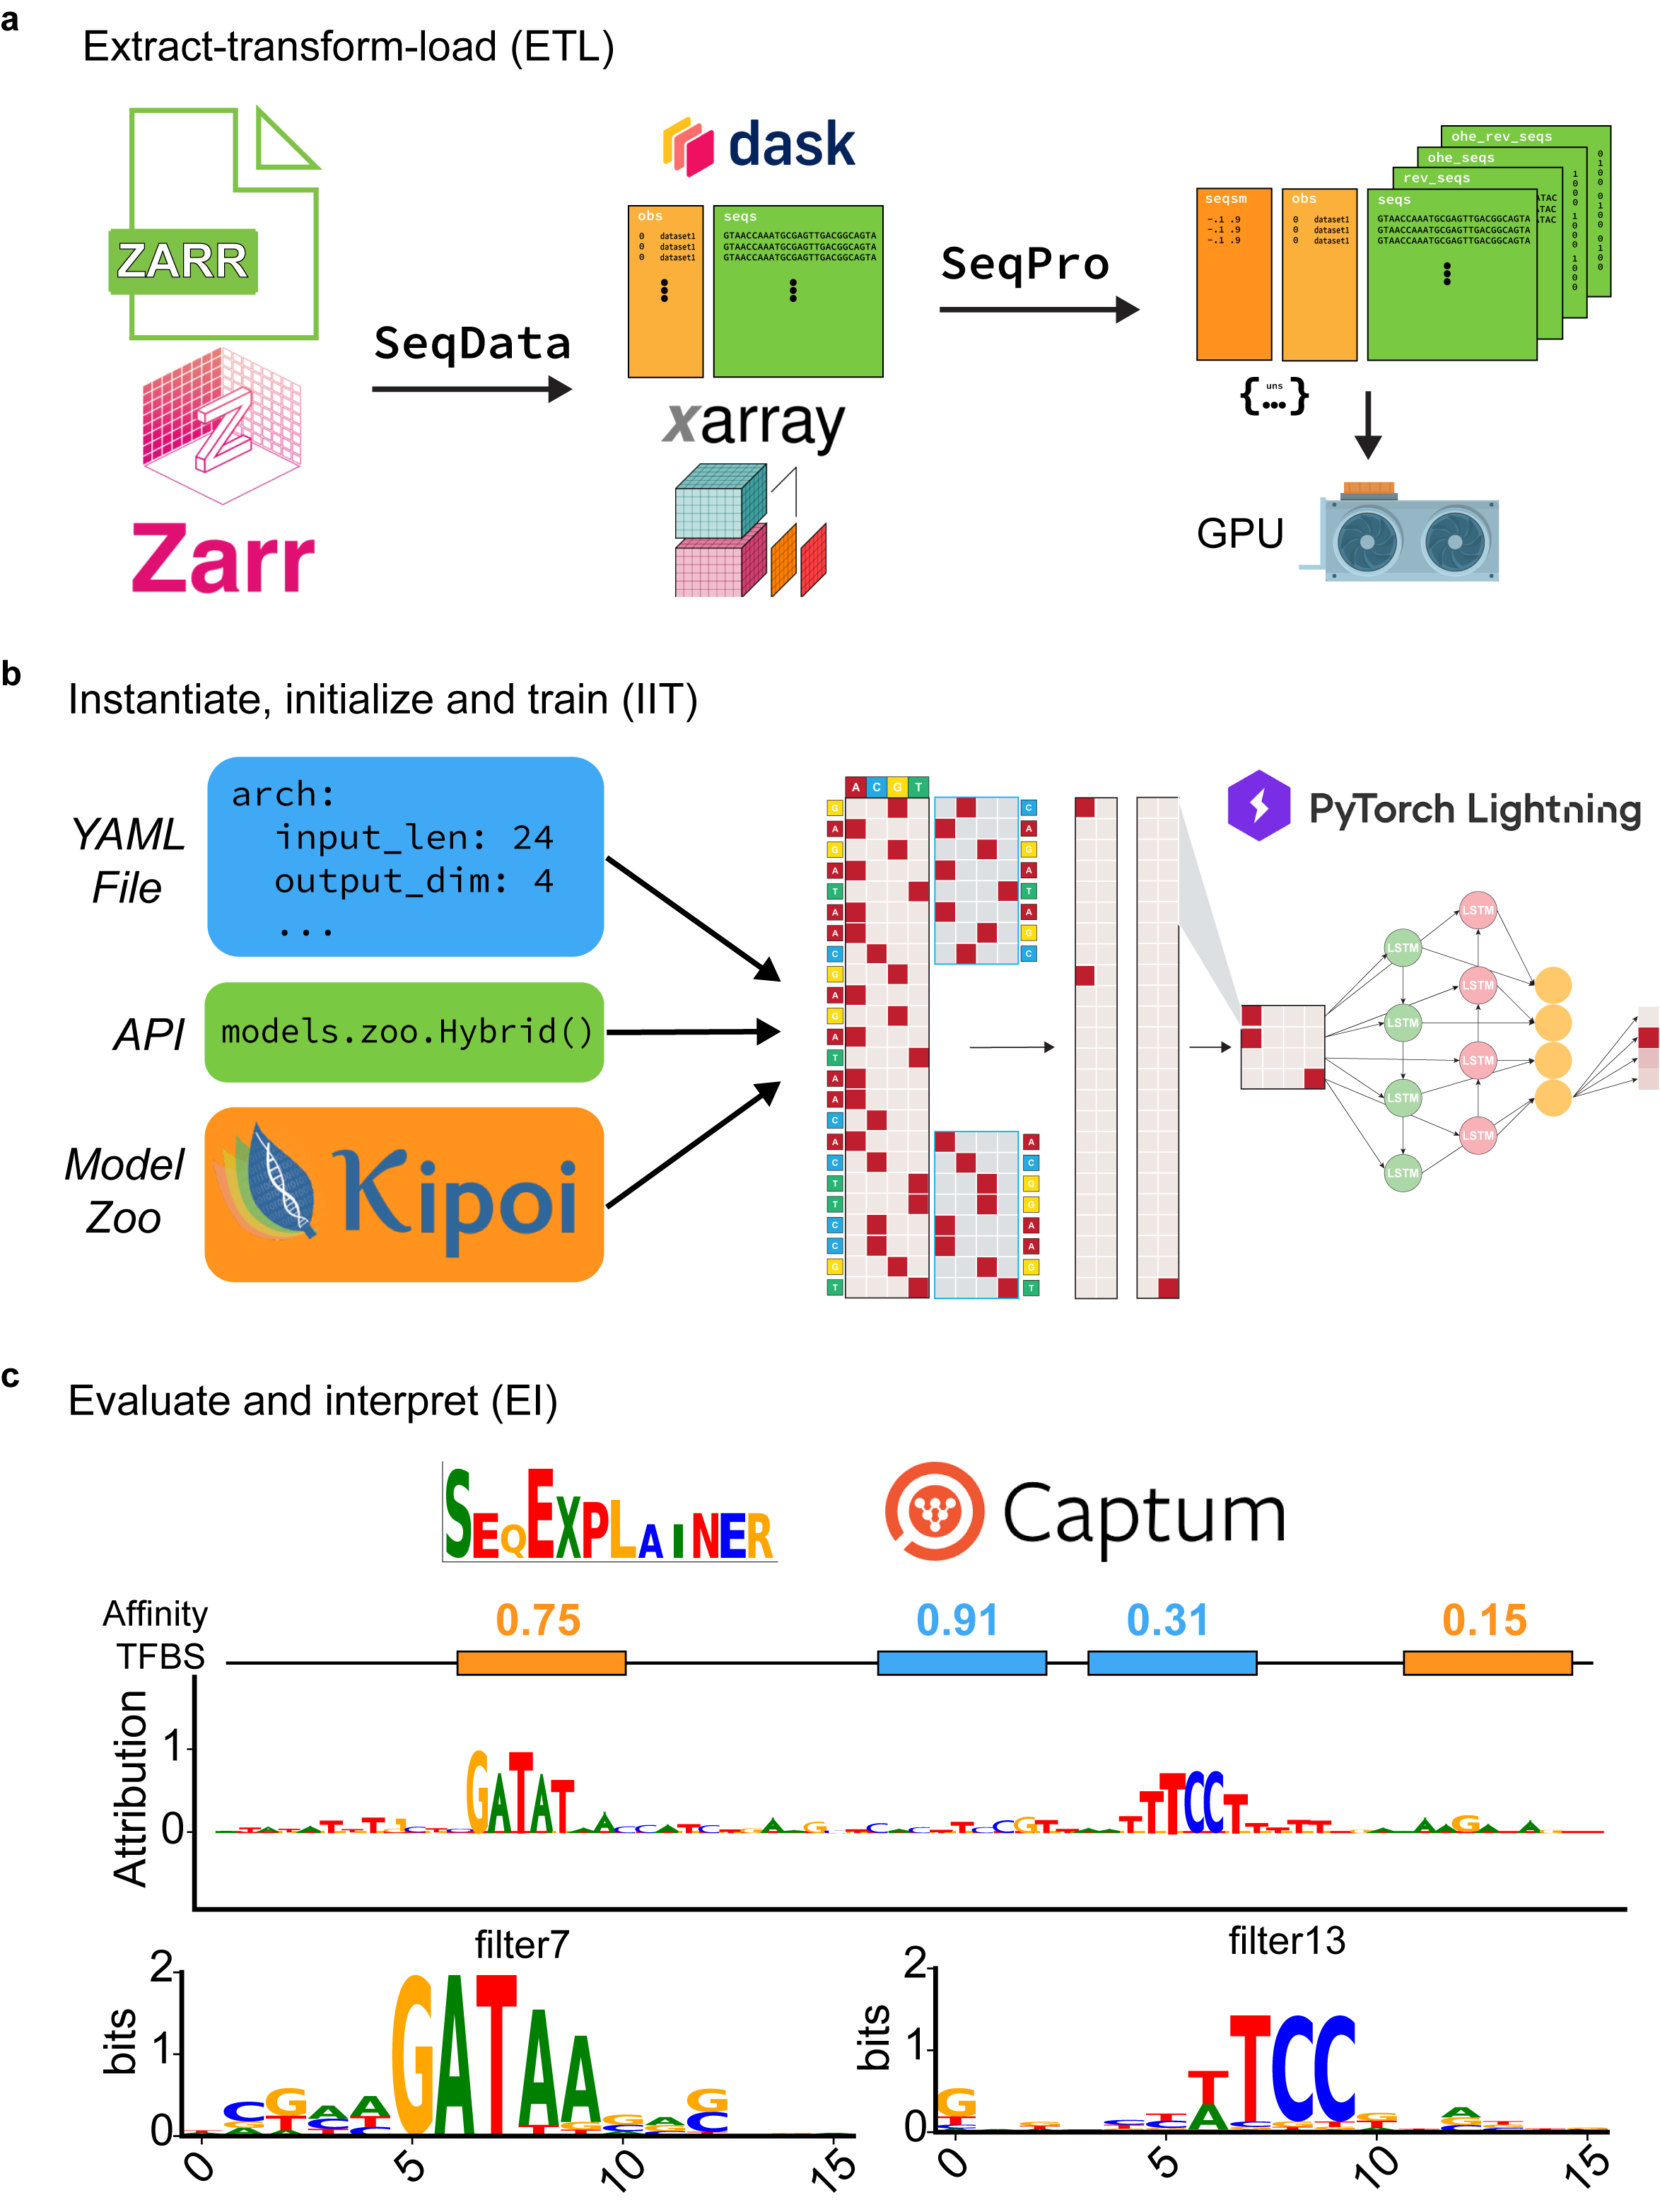
\includegraphics[width=0.9\textwidth, height=0.745\textheight]{1_figures-and-files/figure1.png}
    \caption[EUGENe workflow overview]{\textbf{EUGENe workflow for predictive analyses of regulatory sequences}. The EUGENe workflow can be broken up into three primary stages: \textbf{a}, data extraction, transformation and loading (ETL), \textbf{b}, model instantiation, initialization and training (IIT), and \textbf{c}, model evaluation and interpretation (EI). The ETL stage (\textbf{a}) begins with using the SeqData subpackage to create Dask enhanced, XArray datasets backed by Zarr stores. Data transformation is handled by the SeqPro subpackage, after which data can be loaded into graphical processing units (GPUs). In the subsequent IIT stage (\textbf{b}), model architectures (such as the example shown in the schematic) are instantiated from configuration files (in YAML format) from the EUGENe application programming interface (API) or from Kipoi. EUGENe then uses PyTorch Lightning for training these architectures. The subpackage SeqExplainer (which is backed by the Captum package) is used for model interpretation in the EI stage (\textbf{c}). Common visualizations produced by SeqExplainer include the logos depicted for an example input sequence (top) or for convolutional filters (bottom).}
    \label{fig:1 Figure 1}
\end{figure}

A standard EUGENe workflow consists of 3 main stages outlined in \textbf{Figure~\ref{fig:1 Figure 1}}: extracting, transforming and loading (collectively ETL) data from common file formats (\textbf{Figure~\ref{fig:1 Figure 1}a}), instantiating, initializing and training (collectively IIT) neural network architectures (\textbf{Figure~\ref{fig:1 Figure 1}b}), and evaluating and interpreting (EI) learned model behavior on held-out data (\textbf{Figure~\ref{fig:1 Figure 1}c}). The major goal of EUGENe is to streamline the end-to-end execution of these three stages to promote the effective design, implementation, validation and interpretation of DL solutions in regulatory genomics. We have listed several common DL for regulatory genomics tasks that can be implemented in an end-to-end fashion with EUGENe (\textbf{Supplementary Table 1}). We next describe three in detail, highlighting the core aspects of the workflow on different data types and training tasks. A more detailed description of the workflow is provided in the Methods section.

\begin{figure}[p]
    \centering
    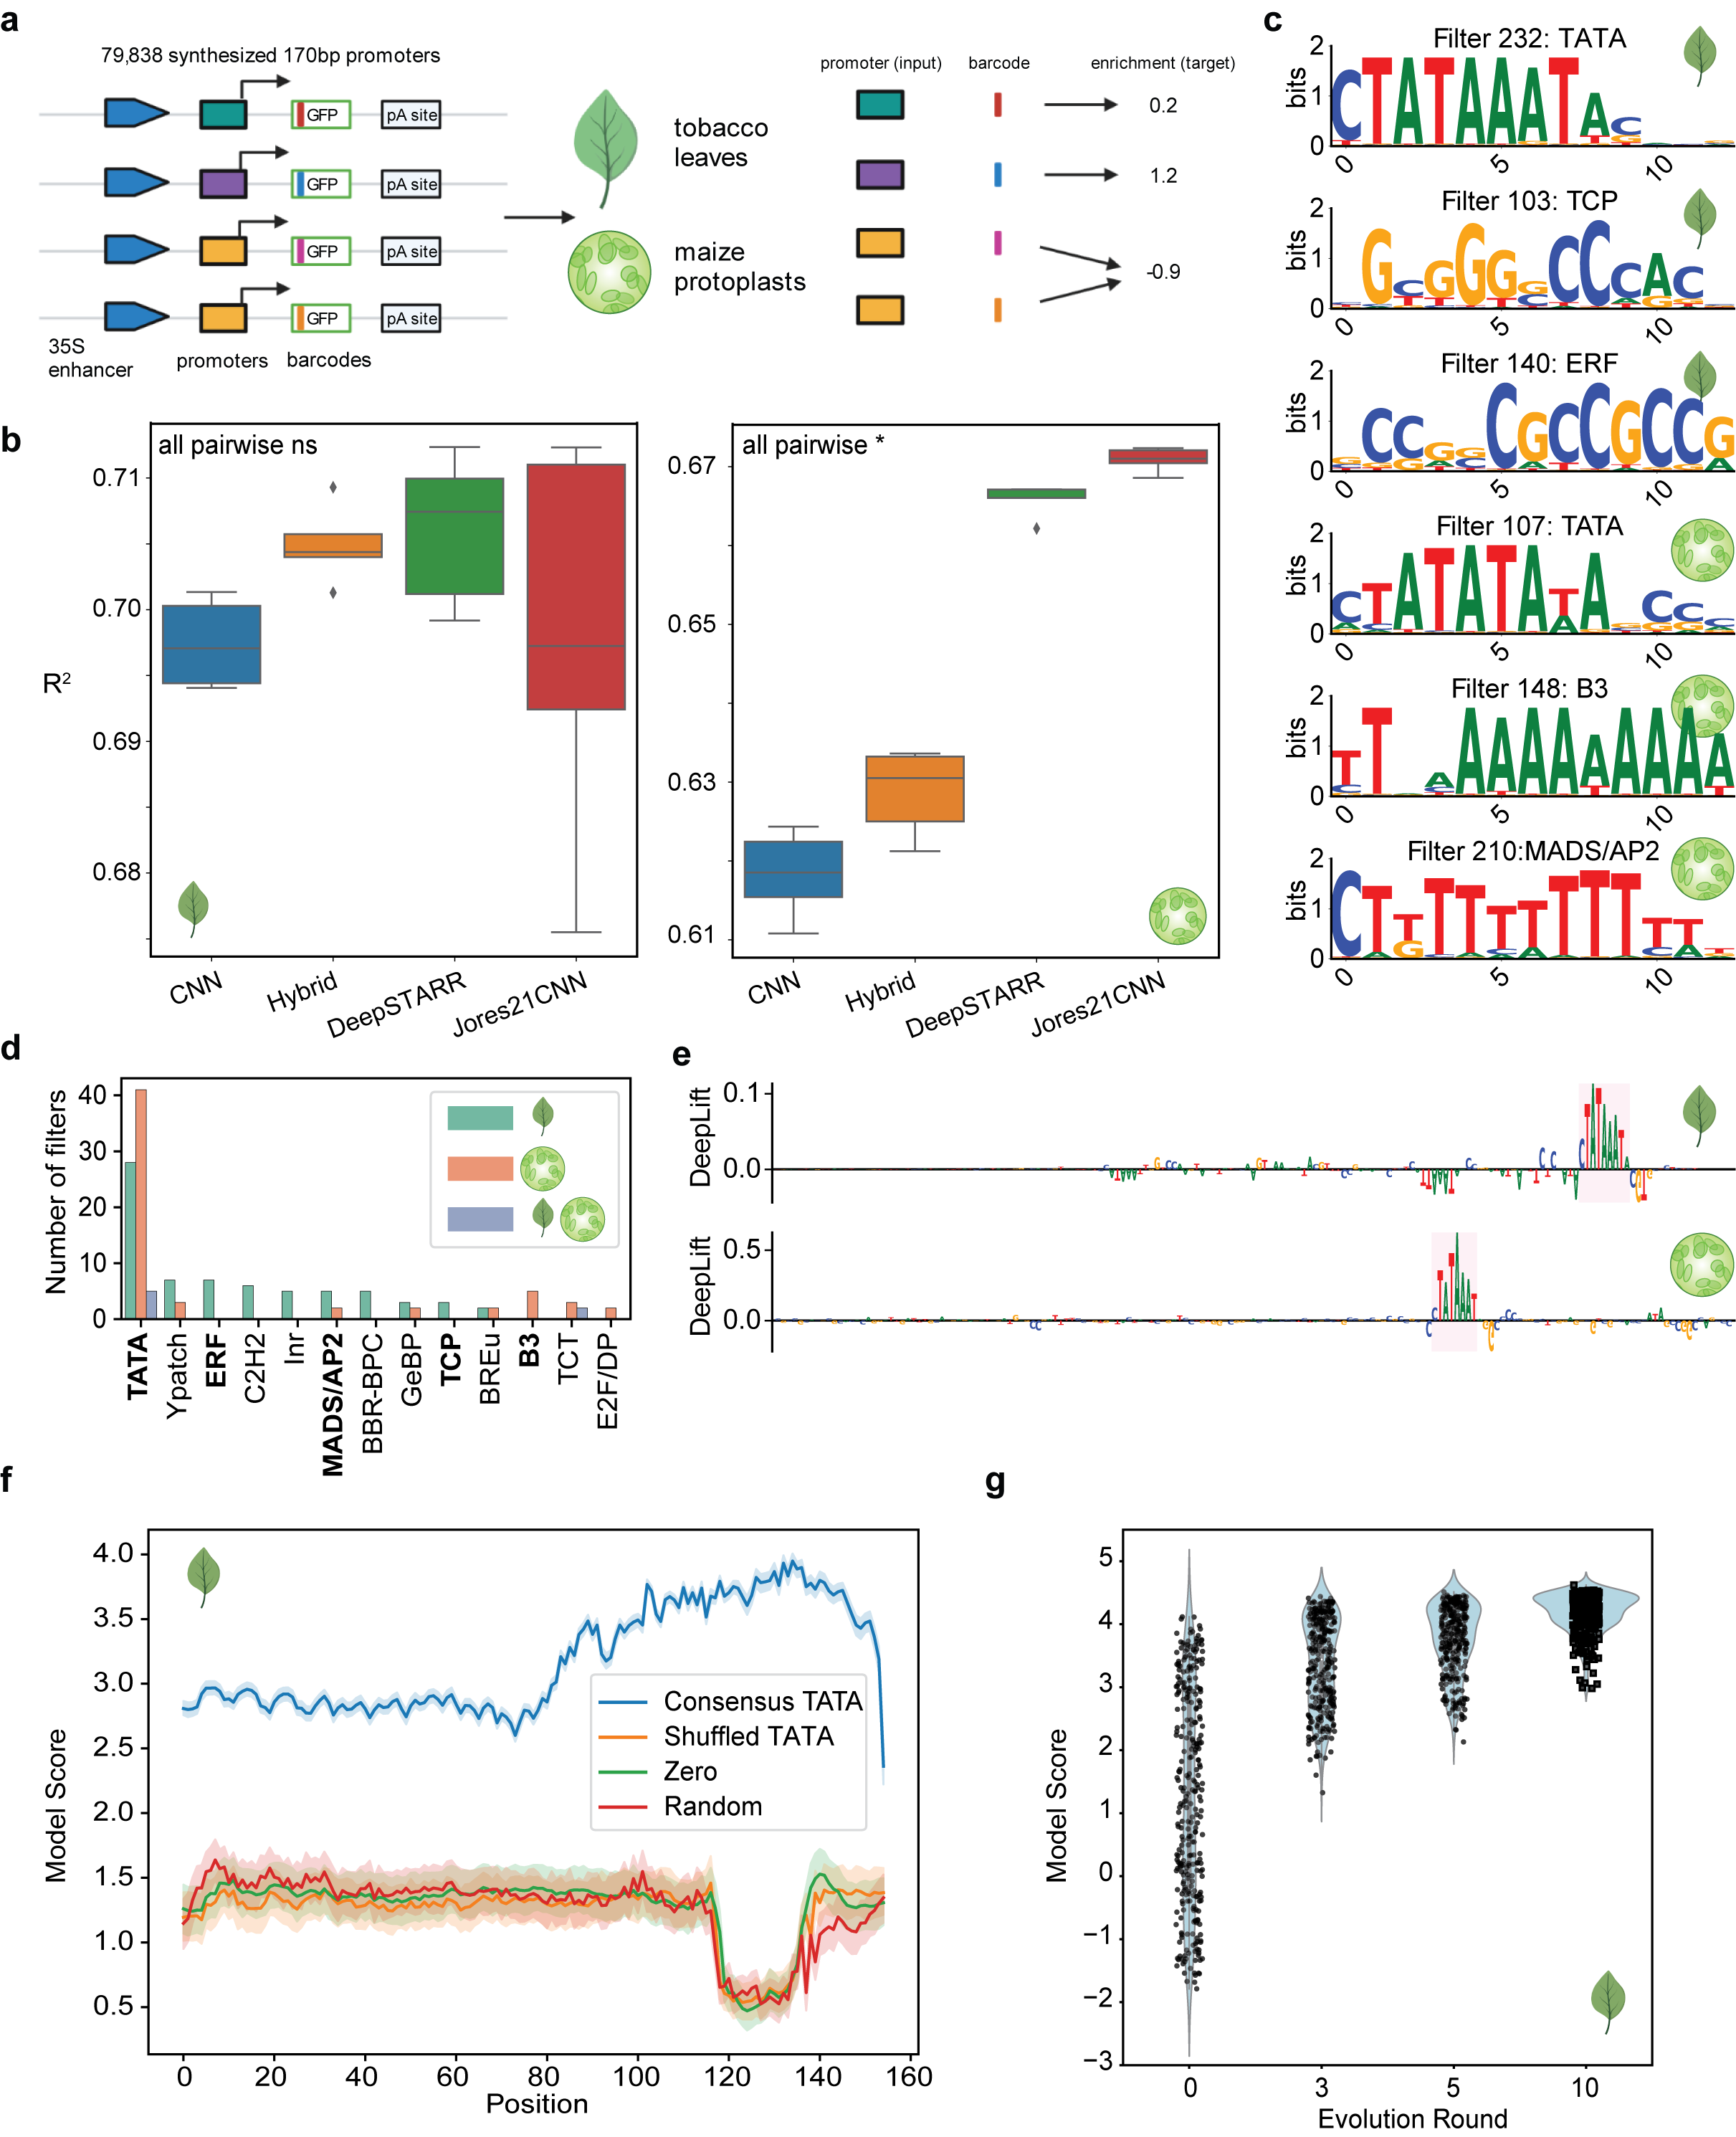
\includegraphics[width=0.9\textwidth, height=0.745\textheight]{1_figures-and-files/figure2.png}
    \caption[STARR-seq plant promoter activity prediction]{\textbf{STARR-seq plant promoter activity prediction}. \textbf{a}, jores21 use case schematic. We trained EUGENe models to predict the regulatory activity of 79,838 plant promoters quantified by plant STARR-seq in tobacco and maize. \textbf{b}, Performance comparison of four convolution-based architectures on predicting promoter activity in tobacco leaves (left) and maize protoplasts (right). The boxplots show distributions of R2 values on held-out test data for each architecture across n=5 independent experiments (random initializations). The boxes show medians along with low and high quartiles. Whiskers extend to the furthest datapoint within 1.5 times the interquartile range. More extreme points are marked as outliers. A two-sided Mann-Whitney U test was used to determine p-values which were adjusted by the Benjamini-Hochberg method (* = p < 0.05, ns = not significant). Test statistics and adjusted p-values for the leaf models (left) were: CNN-Hybrid (u=15, adjusted p-value=0.01), CNN-DeepSTARR (u=24, adjusted p-value=0.17), CNN-Jores21CNN (u=12, adjusted p-value=1.0), Hybrid-DeepSTARR (u=17, adjusted p-value=1.0), Hybrid-Jores21CNN (u=22, adjusted p-value=1.0), DeepSTARR-Jores21CNN (u=14, adjusted p-value=0.84). Test statistics and adjusted p-values for the protoplast models (right) were: CNN-Hybrid (u=15, adjusted p-value=0.03), CNN-DeepSTARR (u=24, adjusted p-value=0.01), CNN-Jores21CNN (u=12, adjusted p-value=0.01), Hybrid-DeepSTARR (u=17, adjusted p-value=0.01), Hybrid-Jores21CNN (u=22, adjusted p-value=0.01), DeepSTARR-Jores21CNN (u=14, adjusted p-value=0.01). \textbf{c}, A hand selected set of convolutional filters visualized as PWM logos that had significant annotations to known core promoter elements (CPE) and transcription factor (TF) binding clusters in plants. \textbf{d}, Histogram showing the number of learned filters assigned to CPEs and TF binding clusters by TomTom with bolded annotations corresponding to the logos in \textbf{c}. \textbf{e}, Sequence logo visualizations of feature importance scores calculated using the DeepLIFT algorithm on the highest predicted test set sequence in the Hybrid leaf (top) and Jores21CNN protoplast (bottom) model. \textbf{f}, Model scores for n=310 sequences implanted with a 16bp sequence containing a consensus TATA box motif, a shuffled version of the same sequence, an all zeros sequence and a random sequence (all 16bp in length). Mean model scores with 95\% confidence intervals are shown. \textbf{g}, Model scores for the same set of n=310 promoters at different rounds of evolution compared against baseline predictions (evolution round 0). The best Hybrid leaf model was used to generate panels \textbf{c}, \textbf{d}, \textbf{f} and \textbf{g} (protoplast model results are shown in Supplementary Figure 1). Source data are provided in the Figure2\_SourceData.zip file.}
    \label{fig:2 Figure 2}
\end{figure}

We first used EUGENe to analyze published data from an assay of plant promoters\cite{Jores2021-iu} (\textbf{Figure~\ref{fig:2 Figure 2}a}). Jores et al selected promoter sequences from -165 to +5-bp relative to the annotated transcription start site (TSS) for protein-coding and microRNA (miRNA) genes of \textit{Arabidopsis thaliana}, \textit{Zea mays} (maize), and \textit{Sorghum bicolor}. A total of 79,838 170-bp promoters were used to transiently transform two separate plant systems, tobacco leaves and maize protoplasts. Regulatory activity was quantified using a variant of the self-transcribing active regulatory region sequencing (STARR-seq) assay\cite{Jores2020-hm} in each system. The resulting data provides two activity scores that can serve as single task regression targets for training EUGENe models.

We implemented both the custom BiConv1D layer\cite{Onimaru2020-do} and CNN architecture (Jores21CNN) described in Jores et al, and then trained separate Jores21CNN architectures for predicting tobacco leaf (leaf models) and maize protoplast (protoplast models) activity scores. We benchmarked these models against built-in CNN and Hybrid architectures with matched hyperparameters, as well as a DeepSTARR architecture\cite{De_Almeida2022-aa} (Supplementary Data 1). As described in Jores et al (see Methods), we initialized 78 filters of the first convolutional layer of all models with position weight matrices (PWMs) of plant transcription factors (n=72) and core promoter elements (n=6)\cite{Jores2021-iu}. In both systems, performance metrics for the most predictive models were comparable to those reported in Jores et al (\textbf{Figure~\ref{fig:2 Figure 2}b}, \textbf{Supplementary Figure~\ref{fig:supplementary_1}a}). We also trained models on activity scores from both leaves and protoplasts (combined models) and noted a marked drop in performance (\textbf{Supplementary Figure~\ref{fig:supplementary_1}b}), underscoring differences in the way the leaf and maize systems interact with the same set of promoters\cite{Jores2021-iu}.

We next applied several of EUGENe’s interpretation functions to the trained models to determine the sequence features each used to predict plant promoter activity. First, we used a filter visualization approach\cite{Minnoye2020-vz} to generate position frequency matrix (PFM) representations for each of the first convolutional layer’s filters and applied the TomTom\cite{Gupta2007-zw} tool to annotate them. We queried the PFMs against the 78 motifs used to initialize the convolutional layers, both to determine if the initialized filters retained their motifs and to see if randomly initialized filters learned them de novo. For the leaf and protoplast models, many of the learned filters were annotated to the TATA box binding motif and other core promoter elements (\textbf{Figure~\ref{fig:2 Figure 2}c}\textbf{d}). Only 10 learned filters from the combined model were assigned a significant annotation by TomTom (\textbf{Figure~\ref{fig:2 Figure 2}d}, \textbf{Supplementary Figure~\ref{fig:supplementary_1}c}), consistent with the observed performance drop in this system (\textbf{Supplementary Figure~\ref{fig:supplementary_1}a}). Next, we applied the DeepLIFT method\cite{Shrikumar2016-lf} to determine the individual nucleotide contributions for each test set sequence prediction. For many of the sequences with the highest observed activity scores, the TATA box motifs were often the lone salient feature identified (\textbf{Figure~\ref{fig:2 Figure 2}e}, \textbf{Supplementary Figure~\ref{fig:supplementary_1}d}). In fact, when only a TATA box motif was inserted into every possible position in each of 310 selected promoters, we observed a 147\% average increase in predicted activity across insertion positions and sequence contexts for the leaf model (\textbf{Figure~\ref{fig:2 Figure 2}f}, \textbf{Supplementary Figure~\ref{fig:supplementary_1}e}). Finally, we performed 10 rounds of in silico evolution on the same set of 310 promoters as described in Jores et al. Almost all starting promoters showed a significant increase in predicted activity after just three mutations (\textbf{Figure~\ref{fig:2 Figure 2}g}, \textbf{Supplementary Figure~\ref{fig:supplementary_1}f}). These results showcase a representative example of the way EUGENe’s interpretation suite can be used to identify the key features that a model uses to make predictions.

\begin{figure}[p]
    \centering
    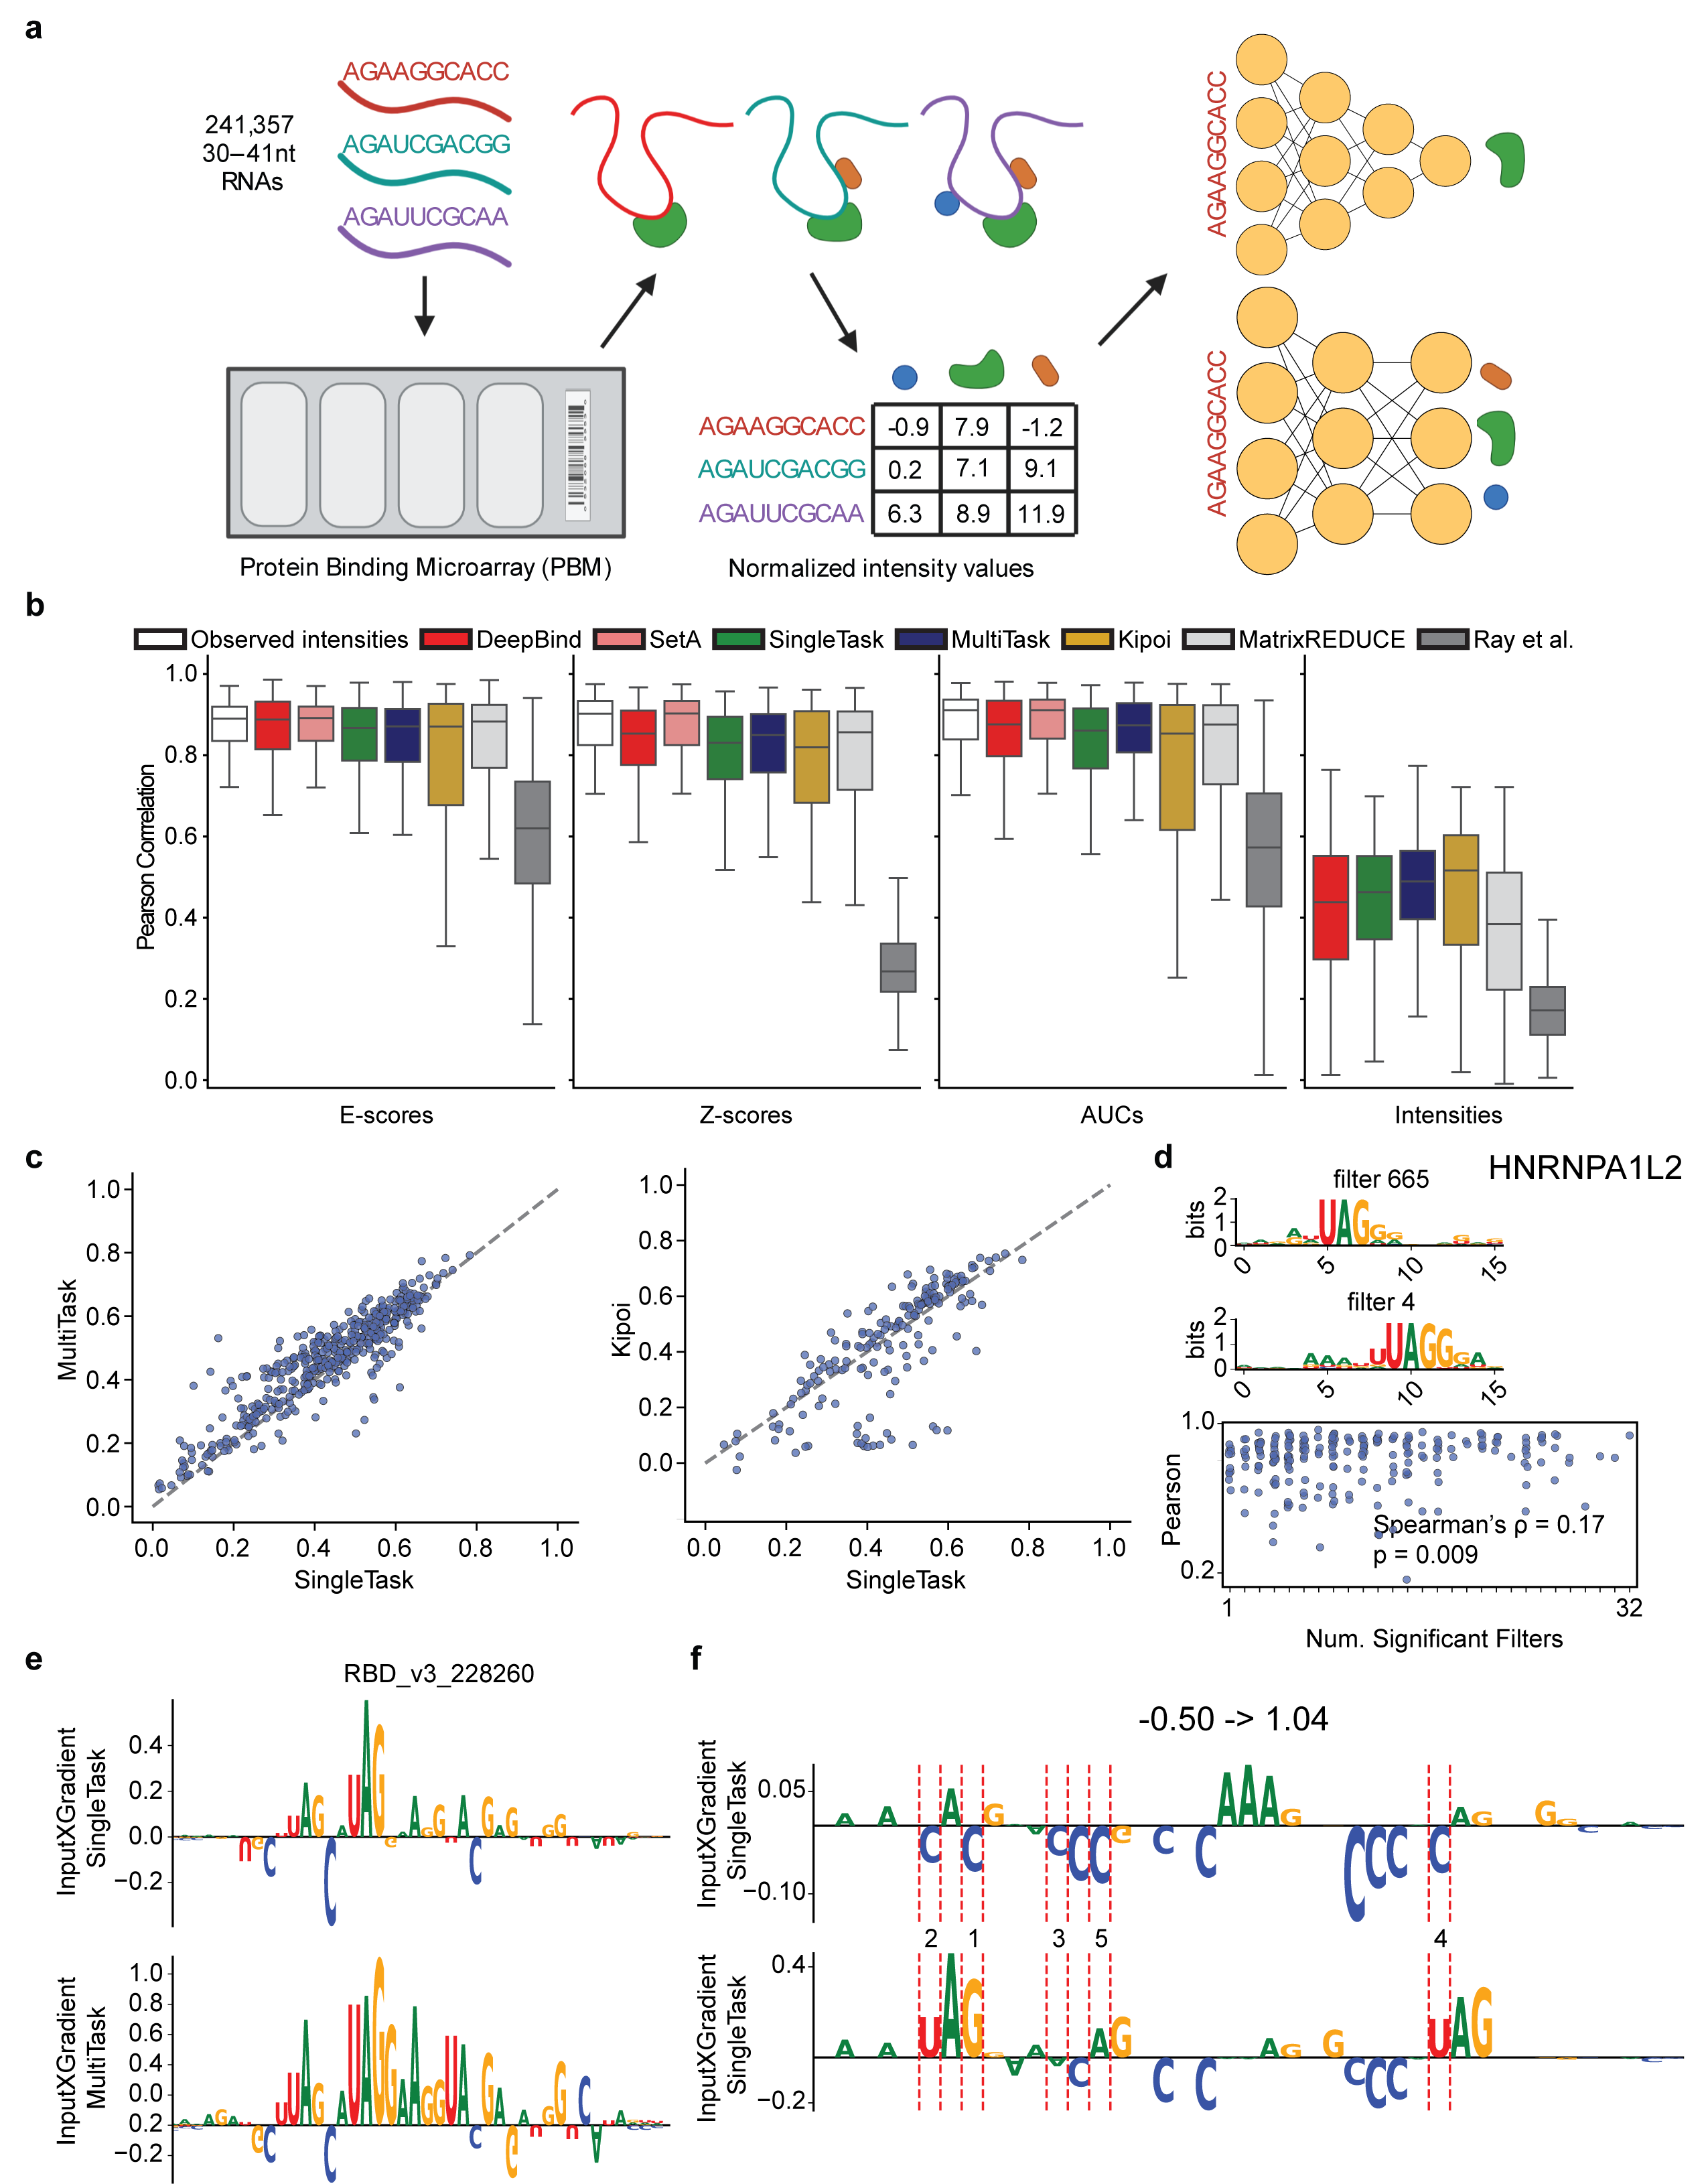
\includegraphics[width=0.9\textwidth, height=0.745\textheight]{1_figures-and-files/extended_data_figure1.png}
    \caption[In vitro RNA binding prediction with DeepBind]{\textbf{In vitro RNA binding prediction with DeepBind}. \textbf{a}, ray13 use case schematic. n=244 RNA binding proteins (RBPs) were assayed across a set of 241,357 RNA probes to generate a 241,357 x 244 dimensional matrix of normalized intensity values. \textbf{b}, Pearson correlations across four different metrics with each metric calculated from comparisons between observed (Set B) and predicted binding intensities (see Methods for more details on how each metric is calculated). Each boxplot indicates a distribution of Pearson correlations across all n=244 RBPs, except for Kipoi which includes n=89 RBPs. Ray et al, MatrixREDUCE, DeepBind and Observed intensities refer to correlations calculated from predicted intensities reported in Alipanahi et al. Observed intensities and SetA refer to correlations calculated using the intensities from Set A probes as the predicted intensities (see Methods). The boxes show medians along with low and high quartiles. Whiskers extend to the furthest datapoint within 1.5 times the interquartile range. \textbf{c}, Performance comparison scatterplots for ST models against MT models (left) and against Kipoi models (right). Each dot indicates a comparison of the Pearson correlation between predicted and observed intensities for two models on a single RBP. \textbf{d}, (top) A multitask filter with a TomTom significant annotation for HNRNPA1L2 visualized as a PWM logo. (middle) A filter for the single task HNRNPA1L2 model with a significant TomTom annotation for HNRNPA1L2. (bottom) The relationship between multitask performance (using the Z-scored Pearson correlations of observed and predicted intensities) on the y-axis, against the number of filters that were annotated with the corresponding RBP for that task on the x-axis. The Spearman’s correlation coefficient and associated p-value are shown. \textbf{e}, Attributions for the sequence with the highest observed intensity in the test set for HNRNPA1L2. The attributions were calculated using InputXGradient for single task (top) and multitask (bottom) models. \textbf{f}, The InputXGradient attribution scores for a random (top) and evolved (bottom) sequence after evolution with the HNRNPA1L2 single task model. Red dashed lines indicate mutations made during evolution and are annotated with the round the mutation occurred in. Source data are provided in the ExtendedFigure1\_SourceData.zip file.}
    \label{fig:3 Figure 3 Figure 3}
\end{figure}

To illustrate EUGENe’s versatility for different inputs and prediction tasks, we next applied it to analyze RNA binding protein (RBP) specificity data introduced in Ray et al\cite{Ray2013-yd} and analyzed with DL in Alipanahi et al\cite{Alipanahi2015-ef}. In the latter work, they trained 244 CNN models (DeepBind models) that each predicted the binding patterns of a single RBP on a set of 241,357 RNA probes (\textbf{Figure~\ref{fig:3 Figure 3 Figure 3}a}). The full probe set was designed to capture all possible RNA 9-mers at least 16 times and was split into two balanced subsets, Set A and Set B, for training and validation respectively (see Methods)\cite{Ray2013-yd}. Each RBP was incubated with a molecular excess of probes from each subset (in separate experiments) and subsequently recovered by affinity purification. The RNAs associated with each RBP were then quantified by microarray and subsequent bioinformatic analysis\cite{Berger2009-la}. This yielded a vector of continuous binding intensity values for each RBP across the probe set that can be used for prediction.

To prepare for training, we first implemented a flexible DeepBind architecture in EUGENe (see Methods), and then trained 244 single task models using a nearly identical training procedure to Alipanahi et al. (Supplementary Data 2). Along with these single task models, we also randomly initialized and trained a multitask model (Supplementary Data 2) to predict 233 RBP specificities (i.e. a 233 dimensional vector) in a single forward pass, excluding 11 RBPs due to a high proportion of missing values across probes in the training set. We also loaded 89 existing Kipoi\cite{Avsec2019-ke} models trained on a subset of human RBPs in the dataset.

Performance on Set B for all deep learning models was on par with Set B’s correlation to Set A (\textbf{Figure~\ref{fig:3 Figure 3 Figure 3}b}, \textbf{Supplementary Figure~\ref{fig:supplementary_2}a}) and both single task and multitask models trained with EUGENe showed comparable performance to Kipoi and DeepBind models (\textbf{Figure~\ref{fig:3 Figure 3 Figure 3}b}\textbf{c}, \textbf{Supplementary Figure~\ref{fig:supplementary_2}a}\textbf{b}). The reason for the poor observed performance of certain Kipoi models is not immediately clear, but could relate to differences in sequence or target preprocessing prior to evaluation. Though the ability to load these pretrained models from Kipoi is very useful for benchmarking, implementing and retraining models is often necessary for fair comparisons of performance. EUGENe supports both loading and retraining models, allowing users to more quickly design and execute quality benchmarking experiments. 

We next applied EUGENe’s interpretation suite to our trained models, first using the filter visualization approach outlined in Alipanahi et al to generate PFMs for convolutional filters. We again used TomTom to identify filters annotated with canonical RBP motifs\cite{Ray2013-yd} in both the best performing single task models and the multitask model (\textbf{Figure~\ref{fig:3 Figure 3 Figure 3}d}, \textbf{Supplementary Figure~\ref{fig:supplementary_2}c}) and found that the number of multitask filters annotated to an RBP was correlated with predictive performance for that RBP (\textbf{Figure~\ref{fig:3 Figure 3 Figure 3}d}, bottom). We also calculated attributions for all Set B sequences using the InputXGradient method\cite{Shrikumar2016-lf} and observed that canonical motifs were learned by both single task and multitask models (\textbf{Figure~\ref{fig:3 Figure 3 Figure 3}e}, \textbf{Supplementary Figure~\ref{fig:supplementary_2}d}). Finally, we used EUGENe’s sequence evolution functionality to evolve 10 random sequences using the single task HNRNPA1L2 model and visualized the attributions for these sequences before and after five rounds of evolution (\textbf{Figure~\ref{fig:3 Figure 3 Figure 3}f}). Several of the mutations that most increased the predicted score were those that generated canonical binding motifs for the protein. We repeated this for two other RBPs (Pcbp2 and NCU02404) and observed that each model prioritizes mutations that create canonical binding motifs specific to the RBP they were trained on (\textbf{Supplementary Figure~\ref{fig:supplementary_2}e}). These results show that EUGENe simplifies the extraction of salient features from models trained within the same workflow.

\begin{figure}[p]
    \centering
    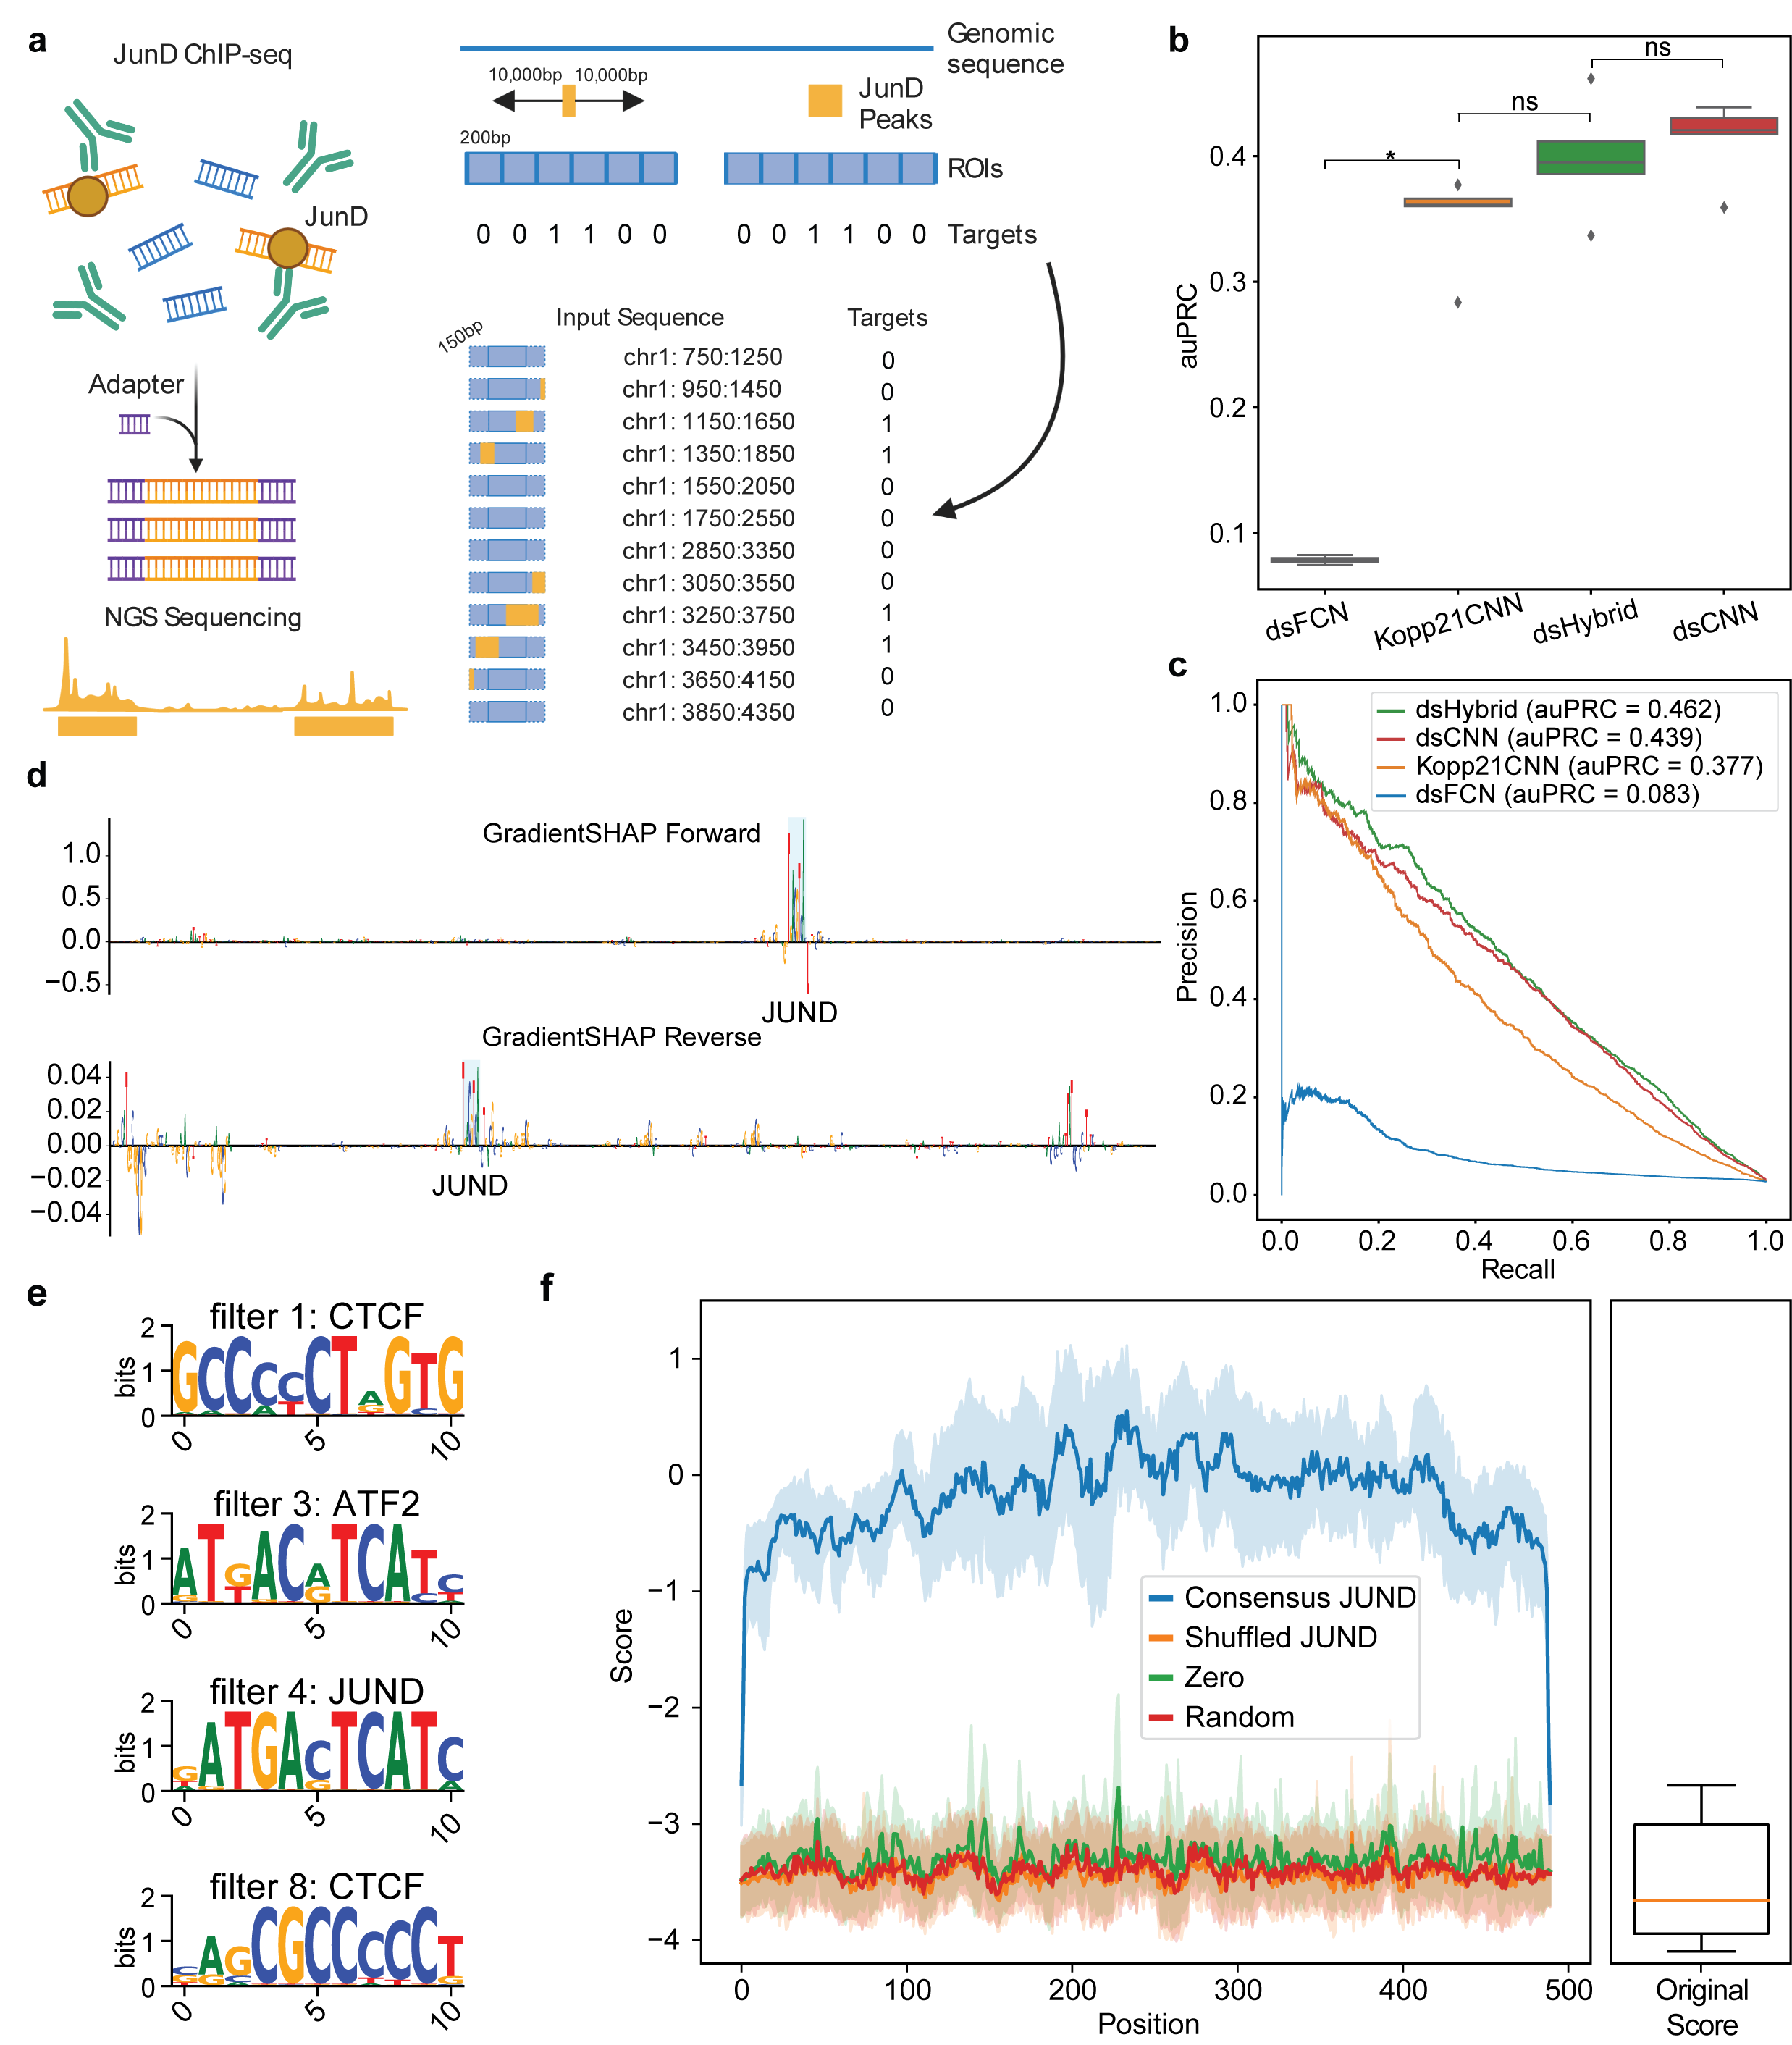
\includegraphics[width=0.9\textwidth, height=0.745\textheight]{1_figures-and-files/extended_data_figure2.png}
    \caption[JunD ChIP-seq binding classification]{\textbf{JunD ChIP-seq binding classification}. \textbf{a}, kopp21 use case schematic. We used SeqData to load in a set of 11,086 ChIP-seq peaks for JunD and to generate positive and negative sets for JunD binding prediction. SeqData uses a set of regions of interest (ROIs) along with peaks and a bin size and outputs a set of labeled sequences for each bin in the ROI. Bins are labeled as positive (1) if they overlap a peak and negative (0) if they do not. Upon loading, each sequence is extended by 150bp in each direction to provide more sequence context for prediction. \textbf{b}, \textbf{c}, auPRCs on held-out test data from chromosome 3 for JunD binding classification across four double-stranded architectures \textbf{b}, The boxplots show distributions of auPRC values on held-out test data for each architecture across n=5 independent experiments (random initializations). A two-sided Mann-Whitney U test was used to determine p-values which were adjusted by the Benjamini-Hochberg method  (* = p < 0.05, ns = not significant). Test statistics and adjusted p-values were: dsFCN-Kopp21CNN (u=0, adjusted p-value=0.02), dsFCN-dsHybrid (u=0, adjusted p-value=0.02), dsFCN-dsCNN (u=0, adjusted p-value=0.02), Kopp21CNN-dsHybrid (u=4, adjusted p-value=0.11), Kopp21CNN-dsCNN (u=4, adjusted p-value=0.11), dsHybrid-dsCNN (u=8, adjusted p-value=0.42). \textbf{c}, auPR curves for the best models from each architecture. \textbf{d}, Sequence logos of attributions for the top predicted sequence. The top row shows attributions from the forward strand and the bottom row from the reverse strand. Attributions were calculated using GradientSHAP. \textbf{e}, A selected set of convolutional filters visualized as PWM logos with significant annotations from TomTom. \textbf{f}, Model scores for n=10 random sequences with consensus JunD motif implanted at each possible location. Mean model scores with 95\% confidence intervals are shown. The boxplot shows the distribution of scores for the random sequences prior to JunD motif implantation. All boxes show medians along with low and high quartiles. Whiskers extend to the furthest datapoint within 1.5 times the interquartile range. More extreme points are marked as outliers. Source data are provided in the ExtendedFigure2\_SourceData.zip file.}
    \label{fig:4 Figure 4}
\end{figure}

As our final use case, we applied EUGENe to the classification of JunD binding as described in Kopp et al\cite{Kopp2020-fw}. This task utilizes ChIP-seq data from ENCODE\cite{ENCODE_Project_Consortium2012-tn} to generate input sequences and binarized classification labels for each sequence (\textbf{Figure~\ref{fig:4 Figure 4}a}). We used EUGENe to first build a DL-ready dataset for this prediction task (see Methods), then implemented the CNN architecture described in Kopp et al (Kopp21CNN). We benchmarked classification performance against built-in FCNs, CNNs, and Hybrid models with matched hyperparameters (Supplementary Data 3). All built-in models were configured to incorporate information from both the forward and reverse strand (double stranded or “ds” models). 

We trained models using the same procedure described in Kopp et al (see Methods)\cite{Kopp2020-fw}. Due to the unbalanced nature of the dataset, we focused on evaluating models with the area under the precision recall curve (auPRC). For our Kopp21CNNs, we were able to achieve comparable performances on held out chromosome 3 sequences to those reported by Kopp et al for one-hot encoded sequences (\textbf{Figure~\ref{fig:4 Figure 4}b}\textbf{c}). The dsFCN, the only model without any convolutional layers, immediately overfit the data after a single training epoch and was not predictive of binding (\textbf{Figure~\ref{fig:4 Figure 4}c}). The dsCNN models, however, achieved higher mean auPRCs than dsHybrid models, and significantly higher auPRCs than Kopp21CNN architectures.

We next applied EUGENe’s interpretation tools to ask whether our best models were learning sequence features relevant to JunD binding to make predictions. We first generated attributions for the forward and reverse complement strands of all test set sequences using the GradientSHAP\cite{Lundberg2017-hh} method and visualized the most highly predicted sequences as sequence logos (\textbf{Figure~\ref{fig:4 Figure 4}d}, \textbf{Supplementary Figure~\ref{fig:supplementary_3}a}). We observed that the most important nucleotides often highlighted consensus or near consensus JunD motifs and that these motifs were often attributed similarly on both the forward and reverse strands (\textbf{Figure~\ref{fig:4 Figure 4}d}, \textbf{Supplementary Figure~\ref{fig:supplementary_3}a}). However, there were instances where salient motifs were highlighted on one strand but not the other (\textbf{Figure~\ref{fig:4 Figure 4}d}), indicating the utility of incorporating information from both strands for prediction. We next generated PFM representations for all 10 filters of each convolutional model (excluding dsFCNs) and annotated them using TomTom against the HOCOMOCO FULL v11 database\cite{Kulakovskiy2018-oz} (\textbf{Figure~\ref{fig:4 Figure 4}e}, \textbf{Supplementary Figure~\ref{fig:supplementary_3}b}). Among the top hits, we found several filters annotated with motifs such as JunD and CTCF (\textbf{Figure~\ref{fig:4 Figure 4}e}, \textbf{Supplementary Figure~\ref{fig:supplementary_3}b}). Finally, we performed an in silico experiment with the best overall model where we slid a consensus JunD motif across each position of a set of 10 randomly generated sequences and predicted binding (\textbf{Figure~\ref{fig:4 Figure 4}f}). We observed that the simple inclusion of the consensus binding site led to a significant jump in predicted output with some position specificity. These results once again showcase that EUGENe’s interpretation methods can help explain model predictions, in this case for DNA protein binding from a genome wide assay.

There are numerous opportunities for future development of EUGENe, but we see a few as high priority. EUGENe is primarily designed to work on nucleotide sequence input (DNA and RNA), but currently does not have dedicated functions for handling protein sequence or multi-modal inputs. Furthermore, as assays move from bulk to single cell resolution, it will be important to develop functionality for handling single cell data that allows users to easily ask questions about cell type specific regulatory syntax. Finally, we plan on expanding EUGENe’s dataset and model library to encompass a larger portion of those available in the field.

The heterogeneity in data types and methods that exist in DL for regulatory genomics and the rapid pace with which the field advances makes maintaining FAIR software in this space a major challenge. One of the tasks in \textbf{Supplementary Table 1}, for instance, involves a recently developed and highly specific data formatting and preprocessing pipeline\cite{Bravo_Gonzalez-Blas2019-fq}. The use of bespoke methods for data preprocessing, as well as for model interpretation, is quite common in the field, and is often necessary to train accurate models that avoid common machine learning pitfalls\cite{Whalen2021-fh}. For example, some workflows may require complex implementations of train and test set splitting to protect against information leakage\cite{Urban2020-ij}. We see substantial value in continuing to extend EUGENe into spaces such as these, and have designed the toolkit to allow for easy integration of this type of functionality. To continue to make bespoke methods and workflows accessible, we intend to encourage community development of EUGENe through tutorials, workshops and a dedicated user-group.

As large consortia (such as ENCODE Phase 4 and Impact of Genomic Variation on Function) and individual groups continue to generate functional genomics data at both the bulk and single cell level, the need for a standardized DL analysis ecosystem to investigate complex relationships in this data becomes even more pressing. We believe that EUGENe represents a positive step in the direction of such an ecosystem and will empower computational scientists to rapidly expand their knowledge, develop and share methods and models, and answer important questions about the genome and how it encodes function.


%%%%%%%%%%%%%%%%%%%%%%%%%%%%%%%%%%%%%%%%%%%%%%%%%%%%%%%%%%%%%%%%%%%%%%%%%%%%%%%%
\section{Methods}
%%%%%%%%%%%%%%%%%%%%%%%%%%%%%%%%%%%%%%%%%%%%%%%%%%%%%%%%%%%%%%%%%%%%%%%%%%%%%%%%

\subsection{The EUGENe workflow}

\begin{figure}[p]
    \centering
    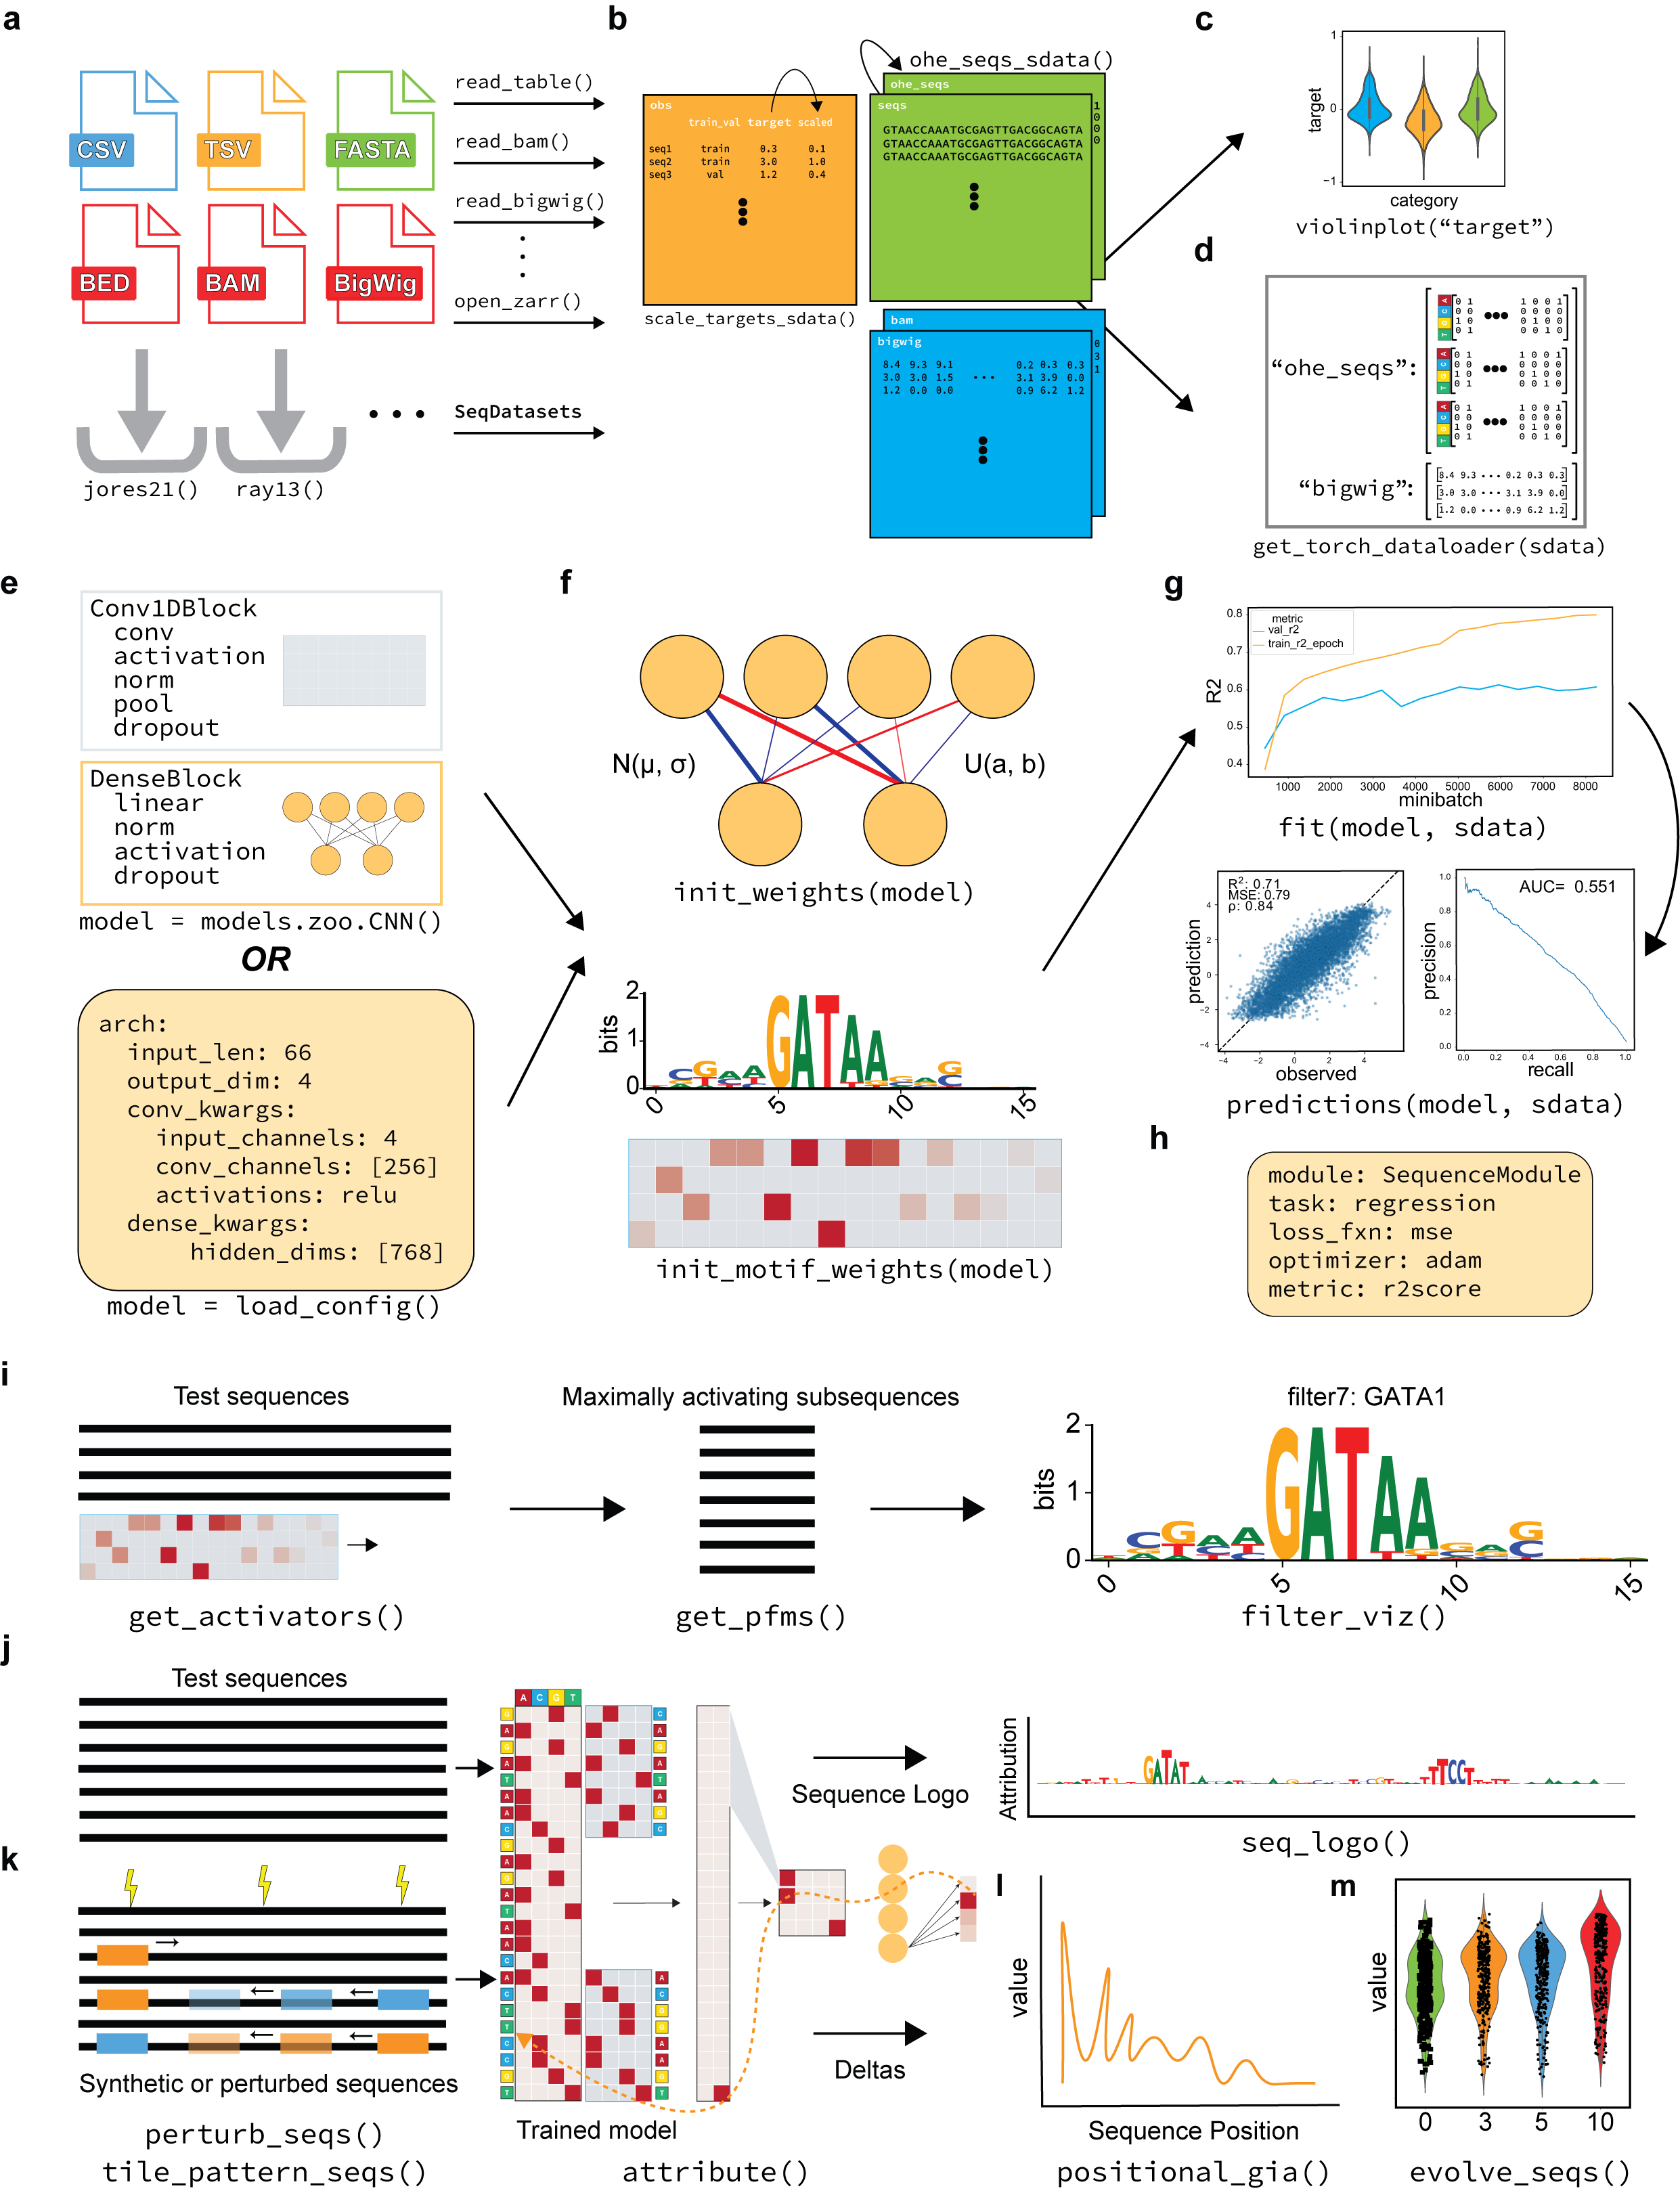
\includegraphics[width=0.9\textwidth, height=0.745\textheight]{1_figures-and-files/extended_data_figure3.png}
    \caption[End-to-end data processing with EUGENe]{\textbf{End-to-end data processing, training, and interpretation with EUGENe}. \textbf{a}, SeqData objects can be loaded from files already on disk, or by calling for a dataset available for download from the SeqDatasets subpackage. Once instantiated, SeqData objects containerize the EUGENe workflow, easing the \textbf{b}, preprocessing of sequences and of sequence metadata, \textbf{c}, the generation of exploratory data analysis plots, and \textbf{d}, the creation of PyTorch loadable datasets and objects. \textbf{e}, An architecture can be instantiated either from a single function call (top) or from a configuration file (bottom). Conv1DBlocks and DenseBlocks both allow for flexibility in the ordering of layers they contain (one example ordering is shown). Instantiated architectures can be \textbf{f}, initialized with a desired initialization scheme, then \textbf{g}, fit to training data and used to predict on held-out data. Performance metric training curves are pictured in the top panel of \textbf{g}, test set performance curves for regression (left) and classification (right) are depicted in the bottom panel of \textbf{g}. Both training and prediction are handled by PyTorch Lightning. We show an example of the arguments for instantiating a SequenceModule in \textbf{h}. \textbf{i}, For filter interpretation, filters in the first convolutional layer are used to scan input sequences for “maximally activating subsequences” that can then be used to generate position frequency matrices and sequence logos. \textbf{j}, Attribution analysis starts by passing inputs sequences through the model to generate an output. This output signal is then backpropagated to the input to generate a per nucleotide score that can be visualized as a sequence logo. \textbf{k}, Random or synthetically designed sequences that have been mutated or have had motifs implanted in them can be scored using a trained model. Results from toy examples of this in silico approach are shown in \textbf{l} and \textbf{m}, which depict a positional importance analysis and a prediction evolution analysis respectively. Example function arguments have been omitted for \textbf{a}, \textbf{b}, \textbf{e}, \textbf{i}, \textbf{j}, \textbf{k}, \textbf{l} and \textbf{m}.}
    \label{fig:5 Figure 5}
\end{figure}

\subsubsection{Data extraction, transformation and loading with SeqData}

The EUGENe workflow begins with extracting data from on-disk formats. Though standardized file formats exist in regulatory genomics, their complexity can make creating model-ready datasets non-trivial. To address this in EUGENe, we created the standalone subpackage SeqData (https://github.com/ML4GLand/SeqData) which flexibly and efficiently reads data from a variety of file formats, including CSV/TSV (tabular), FASTA, BED, BAM, and BigWig (\textbf{Figure~\ref{fig:5 Figure 5}\textbf{a}}, top). The versatility of SeqData enables the generation of many custom datasets from combinations of these file types, including several commonly utilized in regulatory genomics. These include datasets derived from combinations of tabular and FASTA files that are suitable for single and multi-task regression and classification (e.g. DeepSTARR\cite{De_Almeida2022-aa}), datasets from genomic coordinates defined in BED files suitable for multi-task binary classification (e.g. DeepSEA\cite{Zhou2015-rk} or Sei\cite{Chen2022-bn}), and datasets from multiple BigWigs and BED files suitable for binned or base-pair resolution regression (e.g. Basenji\cite{Kelley2018-if} and BPNet\cite{Avsec2021-sw} respectively). EUGENe also supplies a growing collection of hand-curated datasets available via the SeqDatasets subpackage (https://github.com/ML4GLand/SeqDatasets) (\textbf{Supplementary Data~4}) that can be downloaded and subsequently loaded into a workflow via a single function call (\textbf{Figure~\ref{fig:5 Figure 5}\textbf{a}}, bottom).

By default, SeqData reads files from disk as XArray datasets\cite{Hoyer2017-jv} backed by Zarr stores\cite{Miles2023-zk} (\textbf{Figure~\ref{fig:1 Figure 1}\textbf{a}}). We chose to use XArray and Zarr as they are scalable, capable of handling high dimensional data, and have been previously utilized in a variety of bioinformatics domains\cite{Baker2023-sp,Marconato2023-kz,Liu2021-km}. Furthermore, Zarr stores can be loaded out-of-core thanks to functionality offered by XArray and Dask\cite{Team2016-qa}, allowing for processing and training of large-scale datasets (\textbf{Supplementary Figure~\ref{fig:supplementary_4}\textbf{a}}). As is standard in DL, training in EUGENe is always done by loading data into GPU memory in batches (when a GPU is available), but is slowed by using the out-of-core functionality on the CPU (\textbf{Supplementary Figure~\ref{fig:supplementary_4}\textbf{b}}). Thus, the decision on whether to first load the dataset into CPU memory prior to training should balance available resources and dataset size. Certain datasets, such as those used to train Enformer\cite{Avsec2021-hh} or Basenji\cite{Kelley2018-if}, will likely require this out-of-core functionality. However, we have found that many useful and large datasets can entirely fit into memory on machines with less than 32GB of RAM (\textbf{Supplementary Data~5}).

Once created, an array of functions can be called directly on these XArray datasets to perform common preprocessing steps. EUGENe includes a baseline set of functions for train and test set splitting (e.g. by chromosome, fraction, or homology\cite{Teufel2023-kn}) and target normalization (e.g. binning, z-score, clamping, etc.) (\textbf{Figure~\ref{fig:5 Figure 5}\textbf{b}}, left). Sequence preprocessing is handled by the SeqPro subpackage (https://github.com/ML4GLand/SeqPro), which includes Numba accelerated\cite{Lam2015-mo} padding and one-hot encoding of DNA and RNA sequences (\textbf{Figure~\ref{fig:5 Figure 5}\textbf{b}}, right), as well as jittering and k-mer frequency preserving shuffling\cite{Jiang2008-li}. EUGENe also fully supports data visualization through the Matplotlib\cite{Hunter2007-es} and Seaborn\cite{Waskom2021-lk} libraries (\textbf{Figure~\ref{fig:5 Figure 5}\textbf{c}}) and conversion of XArray datasets to formats ingestible by deep learning frameworks in a highly flexible manner (\textbf{Figure~\ref{fig:5 Figure 5}\textbf{d}}). Finally, XArray datasets can easily be converted to more familiar Python data structures (NumPy arrays, Pandas DataFrames, etc.) and back to enable the user to access the functionality of these libraries.

\subsubsection{Model training with PyTorch and PyTorch Lightning}

Designing and training neural networks for regulatory genomics requires a comprehensive library of architecture building blocks. EUGENe builds on the PyTorch library of neural network layers by adding several useful layers such as inception and residual layers. Additionally, EUGENe provides flexible functions for instantiating common "blocks" and "towers" that are composed of heterogeneous sets of layers arranged in a predefined or adaptable order. For instance, a convolutional block (Conv1DBlock in EUGENe) often comprises convolutional, normalization, activation, and dropout layers in different orderings depending on the model and task (\textbf{Figure~\ref{fig:5 Figure 5}\textbf{e}}, top). On top of this, EUGENe’s library supports customizable fully connected (FCN), convolutional (CNN), recurrent (RNN) and hybrid (a combination of the three, shown in \textbf{Figure~\ref{fig:1 Figure 1}\textbf{b}}) architectures that can be instantiated from single function calls or from configuration files (\textbf{Figure~\ref{fig:5 Figure 5}\textbf{e}}, bottom and \textbf{Supplementary Data~6}, basic architectures). We have also constructed several published architectures that represent specific configurations of these basic architectures, and made them accessible to users through single function calls (\textbf{Supplementary Data~6}). Users looking to use their own custom architectures can also do so, as EUGENe only requires that an architecture be defined by its layers and how inputs are propagated through those layers (\textbf{Supplementary Figure~\ref{fig:supplementary_5}\textbf{b}}). In summary, model architectures can be instantiated from the API, built from scratch using our library, or imported from external repositories or packages. We provide a detailed tutorial on instantiating architectures via these different mechanisms in EUGENe’s tutorials repository (\url{https://github.com/ML4GLand/tutorials/blob/main/eugene/models/instantiating_models.ipynb}).

Once instantiated, architectures can be initialized with parameters sampled from standard initialization distributions (\textbf{Figure~\ref{fig:5 Figure 5}\textbf{f}}, top), or in the special case of convolutional filters, initialized with known motifs\cite{Quang2016-ll,Janssens2022-vy} (\textbf{Figure~\ref{fig:5 Figure 5}\textbf{f}}, bottom). EUGENe can then be used to fit initialized architectures to datasets (with the option to perform hyperparameter optimization through the RayTune package\cite{Moritz2017-tm}) and to assess performance and generalizability on held-out test data (\textbf{Figure~\ref{fig:5 Figure 5}\textbf{g}}). For training, EUGENe uses the PyTorch Lightning (PL) framework\cite{Falcon2020-zq} and programmatic objects called LightningModules. Each EUGENe LightningModule delineates the architecture types it can train and standardizes boilerplate tasks for those architectures (e.g. optimizer configuration, metric logging, etc.). For instance, the primary LightningModule in EUGENe, termed SequenceModule (\textbf{Figure~\ref{fig:5 Figure 5}\textbf{h}}), anticipates training an architecture that takes in a single tensor (typically one-hot encoded DNA sequences) and delivers a single tensor output. We have also implemented a ProfileModule for BPNet-style\cite{Avsec2021-sw} training, where models produce multiple tensor outputs (or “heads”), accept optional control inputs, and use multiple loss functions (\url{https://github.com/ML4GLand/use_cases/blob/main/BPNet/train_eugene.ipynb}). Using LightningModules in this manner requires only minor code modifications to allow for the reuse of the same architectures in different training schemes and tasks (\textbf{Supplementary Figure~\ref{fig:supplementary_5}\textbf{b}}) and for the fine-tuning of pretrained models (\textbf{Supplementary Figure~\ref{fig:supplementary_5}\textbf{c}}). We plan on continuing to develop the library of LightningModules for different training schemes, including adversarial learning\cite{Koo2019-dw}, generative modeling\cite{Taskiran2022-zj}, language modeling\cite{Ji2021-mj}, and more.

\subsubsection{Model interpretation with SeqExplainer}

Interpreting models is of critical importance in regulatory genomics\cite{Koo2020-vz,Novakovsky2022-ft,Talukder2021-wj}, but is often made challenging by the complexity of neural networks and methods for their interpretation. To address this in EUGENe, we created a standalone subpackage called SeqExplainer which makes various post-hoc interpretation strategies accessible to most PyTorch models trained on one-hot encoded genomic sequences (\url{https://github.com/ML4GLand/SeqExplainer}). SeqExplainer currently provides functionality for filter interpretation, attribution analysis, in silico experimentation, and sequence generation. Each strategy is briefly detailed below.

The interpretation of learned convolutional filters, commonly employed for model architectures that begin with a convolutional layer, involves using the set of sequences that significantly activate a given filter (maximally activating subsequences) to generate a position frequency matrix (PFM) (\textbf{Figure~\ref{fig:5 Figure 5}\textbf{i}}). The PFM can then be converted to a position weight matrix (PWM), visualized as a sequence logo, and annotated with tools like TomTom\cite{Gupta2007-zw} using databases of known motifs such as JASPAR\cite{Castro-Mondragon2022-kx} or HOCOMOCO\cite{Kulakovskiy2018-oz}. Filter interpretation in this manner does have limitations. TomTom can be inaccurate when annotating motifs from learned filters\cite{Ullah2021-th,Koo2019-fb} and this analysis does not specify the importance of each filter for model predictions\cite{Koo2019-fb}. Despite these limitations, filter interpretation can be useful for hypothesis generation and for further exploration of how architecture affects learned representations\cite{Koo2019-fb,Koo2021-gs,Ploenzke2018-ng}.

Attribution analysis involves using the trained model to score every nucleotide of the input on how it influences the downstream prediction for that sequence (\textbf{Figure~\ref{fig:5 Figure 5}\textbf{j}}). In SeqExplainer and EUGENe, we currently implement several common attribution approaches. These include standard in silico saturation mutagenesis (ISM), InputXGradient\cite{Shrikumar2016-lf}, DeepLIFT\cite{Shrikumar2016-lf}, and GradientSHAP\cite{Lundberg2017-hh}, with the latter three using functionality from the Captum package\cite{Kokhlikyan2020-mv}. Attributions can also be used to validate that the model has learned representations that resemble motifs. Unlike the filter interpretability approach described above, attributions are directly linked to model predictions, and can naturally be extended to model the effects of single nucleotide polymorphisms. However, attributions represent a “local,” often noisy\cite{Han2022-pi,Majdandzic2022-eu} interpretation of a single sequence, and can require clustering into “global” attributions for cleaner interpretation. In SeqExplainer, we offer wrappers for running the popular TF-MoDISco algorithm\cite{Shrikumar2018-sb} to accomplish this.

Attribution analysis, though very useful, stops short of quantifying the effect of whole motifs on model predictions. To get at the quantitative effects of such patterns, EUGENe offers a wide range of functionality for conducting in silico experiments with motifs of interest\cite{De_Almeida2022-aa,Avsec2021-sw}, also known as global importance analyses or GIAs\cite{Koo2021-ly}. Since the space of possible GIAs is essentially infinite, and the type of GIA used is often dependent on the data, model and biological question being asked, we provide the building blocks for GIAs in SeqExplainer, including functionality for generating background sequences and introducing perturbations (e.g., mutations, motif embedding, motif occlusion, etc.) to those sequences (\textbf{Figure~\ref{fig:5 Figure 5}\textbf{k}}). EUGENe currently offers high-level functions for streamlining positional importance analysis (\textbf{Figure~\ref{fig:5 Figure 5}\textbf{l}}) and distance-dependent motif cooperativity analysis, and we anticipate adding many more common GIAs to EUGENe in the future.

The last class of interpretability methods currently offered in EUGENe uses trained models to guide sequence evolution. We implement the simplest form of this approach that iteratively evolves a sequence by greedily inserting the mutation with the largest predicted impact at each iteration. Starting with an initial sequence (e.g., random, shuffled, etc.), this strategy can be used to evolve synthetic functional sequences\cite{Taskiran2022-zj} (\textbf{Figure~\ref{fig:5 Figure 5}\textbf{m}}). This style of analysis is a promising direction for further research and can also be used for validating that the model has learned representations that resemble motifs.

\subsection{Analysis of plant promoter data}

\subsubsection{Data acquisition and preprocessing}

Plant promoter assay data were obtained from the GitHub repository associated with Jores et al. These included two identical libraries for a set of 79,838 plant promoters synthesized with an upstream viral 35S enhancer and downstream barcode-tagged GFP reporter gene (\textbf{Figure~\ref{fig:2 Figure 2}\textbf{a}}). The libraries were designed to include 10–20 constructs with distinct barcodes for each promoter. These libraries were used to transiently transform both tobacco leaves and maize protoplasts, and promoter activities were assayed using plant STARR-seq\cite{Jores2020-hm}. Per-barcode activity was calculated as the ratio of RNA barcode frequency to DNA barcode frequency, and the median of these ratios was then used to aggregate across barcodes assigned to the same promoter. These aggregated scores were then normalized by the median value for a control construct and were log-transformed to calculate a per-promoter “enrichment” score. We downloaded these enrichment scores from the authors’ GitHub repository (\url{https://github.com/tobjores/Synthetic-Promoter-Designs-Enabled-by-a-Comprehensive-Analysis-of-Plant-Core-Promoters/tree/main/CNN}) for both libraries as separate datasets to use as training targets. We used the identical 90/10 training and test split used in Jores et al. (the dataset could be downloaded with set labels). The training set was further split into 90/10 train and validation sets. All sequences were one-hot encoded using a channel for each letter of the DNA alphabet (“ACGT”).

\subsubsection{Model initialization and training}

We implemented the Jores21CNN architecture by translating the Keras code in the associated GitHub repository into PyTorch and integrating it into our library. We benchmarked this architecture against built-in CNN, Hybrid, and DeepSTARR architectures in EUGENe with the hyperparameters described in \textbf{Supplementary Data~1}. In each convolutional layer, the Jores21CNN first applies a set of filters to the input as is standard for convolutional models, but also applies the reverse complements of the filters (as opposed to the reverse complement of the sequences) to each input in an effort to capture information from both strands\cite{Onimaru2020-do}. Since this still only requires a single strand as input into the models, we opted to benchmark against only single-stranded versions of built-in CNN and Hybrid models. Following instantiation, we initialized 78 filters in the first convolutional layer of each model using PWMs derived from core promoter elements and transcription factor binding clusters downloaded from the authors’ GitHub repository (\url{https://github.com/tobjores/Synthetic-Promoter-Designs-Enabled-by-a-Comprehensive-Analysis-of-Plant-Core-Promoters/tree/main/data/misc}). All other parameters were initialized by sampling from the Kaiming normal distribution\cite{He2015-qh}. We trained models for a maximum of 25 epochs with a batch size of 128 and used the Adam optimizer with a starting learning rate of 0.001. A learning rate scheduler with a patience of 2 epochs was included to adaptively decrease the learning rate. We used mean squared error as our objective function and stopped training early if the validation set error did not decrease after 5 epochs.

\subsubsection{Model evaluation and interpretation}

Models were primarily evaluated using the percentage of variance explained ($R^2$) on predictions for the test set. We repeated the above training procedure across 5 independent random initializations and evaluated $R^2$ scores across these trials. For PWM visualization, we used the approach described in Minnoye et al.\cite{Minnoye2020-vz} Briefly, for each filter in the first convolutional layer, we calculated activations for all subsequences (of the same length as the filter) within the test set sequences. We then took the top 100 subsequences corresponding to the top 100 activations (maximally activating subsequences) and generated a PFM. For visualizing filters as sequence logos, we converted PFMs to PWMs using a uniform background nucleotide frequency. We calculated attributions for all test set sequences using the DeepLIFT method\cite{Shrikumar2016-lf}. To perform the feature implantation approach, we downloaded the 16bp PFM containing the consensus TATA box motif from the Jores et al. GitHub repository and one-hot encoded it by taking the highest probability nucleotide at each position. We also downloaded the set of 310 promoters (\url{https://github.com/tobjores/Synthetic-Promoter-Designs-Enabled-by-a-Comprehensive-Analysis-of-Plant-Core-Promoters/blob/main/analysis/validation_sequences/promoters_for_evolution.tsv}) used in Jores et al. for in silico evolution. We then implanted the TATA box-containing sequence at every possible position of each of the 310 promoter sequences and used selected high-performing models (one each from leaf, protoplast, and combined) to make predictions. We compared this to predicted scores generated with the same feature implantation approach using a shuffled version of the 16bp sequence containing the TATA box motif, a random 16bp one-hot encoded sequence, and a 16bp all-zeros input. We performed the in silico evolution experiments on the same set of 310 promoter sequences\cite{Jores2021-iu}. In each round, we first used in silico saturation mutagenesis to identify the mutation that increased the model score by the largest positive value (delta score). We then introduced this mutation into the sequence and repeated this for 10 iterations.

\subsection{Analysis of RNA binding data}

\subsubsection{Data acquisition and preprocessing}

As described in detail in Alipanahi et al.\cite{Alipanahi2015-ef}, a set of 241{,}357 31--41\,nt RNA probes were split into two experimental sets, Set A and Set B, with each designed to include all possible 9-mers at least eight times, all possible 8-mers at least 33 times, and all possible 7-mers at least 155 times (\textbf{Figure~\ref{fig:3 Figure 3 Figure 3}\textbf{a}}). These probes were assayed against 244 RBPs using a protein binding microarray (PBM)\cite{Berger2009-la}, and intensities were normalized as described in Ray et al.\cite{Ray2013-yd}. We downloaded the normalized RNA probe binding intensity matrix from the Ray et al. supplementary data repository (\url{http://hugheslab.ccbr.utoronto.ca/supplementary-data/RNAcompete_eukarya/norm_data.txt.gz}) and separated the Set A and Set B sequences into two distinct groups. To remove outliers, we capped all probe intensity values at the 99.95th percentile for each RBP, and then Z-scored the clamped values to have zero mean and unit variance. All normalizations were performed using Set A statistics (i.e., Set B values were normalized using the means and standard deviations from Set A). For multitask prediction, we excluded 11 RBPs with $\geq$0.1\% missing values across Set A and removed all Set A probes with missing values for any of the remaining 233 RBPs. This resulted in 120{,}326 and 110{,}645 probes for training single-task and multitask models, respectively, and 121{,}031 probes in Set B for testing. Set A was then further split 80/20 into training and validation sets. All input sequences were one-hot encoded across the RNA alphabet (“ACGU”).

\subsubsection{Model initialization and training}

We implemented the DeepBind architecture described in the Supplementary Information (\url{https://static-content.springer.com/esm/art%3A10.1038%2Fnbt.3300/MediaObjects/41587_2015_BFnbt3300_MOESM51_ESM.pdf}) of Alipanahi et al.\ and added it to the EUGENe model library. DeepBind architectures were initially designed to take either the forward strand or both strands (ds) as input. However, since Alipanahi et al.\ trained their RBP models with just the single strand input (due to the single-stranded nature of RNA), we also used a single-stranded implementation for our DeepBind models. We initialized both the single-task models and the multitask model with parameters sampled from the Kaiming normal distribution\cite{He2015-qh} and trained all models for a maximum of 25 and 100 epochs, respectively, using the Adam optimizer\cite{Kingma2014-kn} and a starting learning rate of 0.005. We included a learning rate scheduler that reduced the learning rate with a patience of 2 epochs. The batch size was fixed to 64 and 1024 for the single- and multitask models, respectively. Mean squared error was used as the objective function, and training was halted early if the validation set error did not decrease after 5 epochs. For multitask models, we used the average mean squared error across all tasks. Hyperparameters for all model architectures are provided in Supplementary Data 2. Finally, we downloaded a set of 89 pretrained human RBP models from Kipoi (\url{https://kipoi.org/models/DeepBind/Homo_sapiens/RBP/}) and wrapped Kipoi functions to make predictions using these models.

\subsubsection{Model evaluation}

We evaluated models using the Z-score, AUC, and E-score metrics reported in Alipanahi et al. To calculate these metrics, we first computed a binary $n \times m$ matrix $A$, where the $n$ rows represent all possible 7-mers from the RNA alphabet (e.g., AAAAAAA, AAAAAAC, AAAAAAG, etc.) and the $m$ columns represent the 121{,}031 probes from Set B. Each entry $a_{ij}$ in the matrix is 1 if the $i$th k-mer is found in the $j$th probe, and 0 otherwise. For a single RBP, we have normalized binding intensity values across the 121{,}031 probes (denoted by the $m$-dimensional vector $x$). We compared each row of $A$ (i.e., each k-mer indicator vector) to $x$ and computed Z-scores, AUCs, and E-scores as described in \cite{Alipanahi2015-ef,Ray2013-yd}. This was repeated for all k-mers to generate an $n$-dimensional vector for each metric, reflecting that k-mer's contribution to binding by the RBP. For Z-scores, a value of 0 indicates average binding when the k-mer is present, with more positive values indicating stronger-than-average binding. AUC and E-scores (a variant of AUC) range from 0 to 1, with values closer to 1 indicating a strong association between k-mer presence and binding intensity. We repeated this procedure using predicted intensities from each model in place of the observed values, yielding a set of $n$-dimensional vectors for each model–metric pair. For each, we calculated Pearson and Spearman correlations with the observed vector $x$ to produce a pair of correlation values per RBP. These values are plotted as individual points in \textbf{Figure~\ref{fig:3 Figure 3}\textbf{b}} and \textbf{Supplementary Figure~\ref{fig:supplementary_2}\textbf{a}}. Repeating this process across all RBPs results in a distribution of performance values for each model.

We applied the same procedure using Set A observed intensities to compute a distribution of correlations serving as a biological replicate baseline. These are shown as the “Set A” and “Observed intensities” columns in \textbf{Figure~\ref{fig:3 Figure 3}\textbf{b}} and \textbf{Supplementary Figure~\ref{fig:supplementary_2}\textbf{a}}. The “Set A” distribution was computed using our own implementation, while the “Observed intensities” distribution was obtained from performance tables in the supplement of Alipanahi et al. Finally, we calculated Pearson and Spearman correlation coefficients between observed and predicted Set B intensities for all models. Because Set A and Set B contain different probe sequences, this comparison could not be performed on Set A, explaining the absence of “Set A” and “Observed intensities” in the final boxplots of \textbf{Figure~\ref{fig:3 Figure 3}\textbf{b}} and \textbf{Supplementary Figure~\ref{fig:supplementary_2}\textbf{a}}.

\subsubsection{Model interpretation}

For filter visualization, we used the approach described in Alipanahi et al. Briefly, for a given filter, we computed activation scores for all subsequences (of the same length as the filter) from Set B probes and identified the maximum activation. We then selected only those subsequences with activations at least three-fourths of this maximum to generate a position frequency matrix (PFM) for that filter. This process was repeated for all 16 filters in each of the top 10 single-task models and for all 1,024 filters of the multitask model. The top 10 single-task models were selected based on Pearson correlation between observed and predicted intensities. We annotated the multitask PFMs using TomTom against the Ray2013 \textit{Homo sapiens} database, retaining hits with Bonferroni-corrected $p$-values $\leq 0.05$. We computed attributions for all Set B probes using the InputXGradient method\cite{Shrikumar2016-lf}. For multitask models, attributions were calculated per task to determine how each input nucleotide contributed to the prediction for a specific RBP. We performed this analysis only for a subset of RBPs, again using Pearson correlation to select the top 10 single-task models and the top 10 best-predicted tasks in the multitask setting. We applied the same \textit{in silico} evolution procedure as described for the plant promoter use case. Using trained models for selected RBPs, we first generated 10 random 41-nt sequences (uniformly sampled from ``ACGT'') and conducted 5 rounds of evolution. In each round, we identified and applied the mutation that most increased model score. We then computed feature attributions for both the original and evolved sequences using the InputXGradient method and compared them.

\subsection{Analysis of JunD binding data}

\subsubsection{Data acquisition and preprocessing}

We followed the same procedure to acquire and preprocess the data for training models on the prediction of JunD binding as reported in Kopp et al.\cite{Kopp2020-fw} We started by downloading JunD peaks from human embryonic stem cells (H1-hESC) called with the hg38 reference genome from \texttt{encodeproject.org} (ENCFF446WOD, conservative IDR thresholded peaks, narrowPeak format). We next defined regions of interest (ROIs) by extending the union of all JunD peaks by 10\,kb in each direction. Blacklisted regions for hg38 (\url{http://mitra.stanford.edu/kundaje/akundaje/release/blacklists/hg38-human/hg38.blacklist.bed.gz}) were removed using \texttt{bedtools}\cite{Quinlan2010-ei}, and the resulting regions were trimmed to ensure divisibility into 200\,bp bins. For training and testing, we binned each ROI into 200\,bp sequences and labeled bins overlapping a JunD binding peak as positive and all others as negative. As input to the models, we extended each 200\,bp bin by 150\,bp on each side (producing a 500\,bp sequence) and one-hot encoded each sequence using one channel per DNA base (``ACGT''). In total, we generated 1,013,080 200\,bp bins to construct the training, validation, and test sets. Sequences were split by chromosome: validation sequences were drawn from chromosome 2, test sequences from chromosome 3, and the remainder were used for training.

\subsubsection{Model initialization and training}

For the JunD binding task, we implemented the Kopp21CNN architecture described in Kopp et al. by replicating the Keras code in their associated GitHub repository and the Supplementary Information \url{https://static-content.springer.com/esm/art%3A10.1038%2Fs41467-020-17155-y/MediaObjects/41467_2020_17155_MOESM1_ESM.pdf}. We trained five random initializations each of dsFCN, dsCNN, dsHybrid, and Kopp21CNN architectures, initializing parameters with the Kaiming normal distribution.\cite{He2015-qh} All models were designed to receive both the forward and reverse strands as input via a shared architecture (ds). Following Kopp et al., we trained each model for a maximum of 30 epochs using the AMSGrad optimizer\cite{Phuong2019-dz} with a starting learning rate of 0.001. The batch size was fixed to 64, and binary cross-entropy was used as the loss function. Training was halted early if the validation loss did not decrease after five consecutive epochs. Hyperparameters for each model are provided in \textbf{Supplementary Data 3}.

\subsubsection{Model evaluation and interpretation}

Models were evaluated using the area under the precision-recall curve (auPRC) metric, as the dataset was substantially imbalanced. Model interpretation was performed using EUGENe’s attribution, filter visualization, and \textit{in silico} experimentation tools. Attributions for the forward and reverse strands of all test set sequences were computed using the GradientSHAP method.\cite{Lundberg2017-hh} For filter visualization, we applied the approach described previously and constructed position frequency matrices (PFMs). These PFMs were submitted to the TomTom webserver for annotation against the HOCOMOCO v11 FULL database,\cite{Kulakovskiy2018-oz} retaining only those hits with a Bonferroni-corrected $p$-value $\leq 0.05$. Logos were rendered using a uniform background nucleotide distribution. We also conducted an \textit{in silico} motif implantation experiment using the JunD PFM from JASPAR (\url{https://jaspar.genereg.net/matrix/MA0491.1}). We generated 10 random sequences by uniform sampling and implanted the one-hot encoded JunD consensus motif at every possible position. We compared predicted scores from these modified sequences to those generated from implanting a shuffled version of the motif, a completely random 10\,bp sequence, and a zero-valued 10\,bp input.

\subsection{Data visualization software}

For most exploratory data analysis and performance evaluations, we used a combination of the Seaborn and Matplotlib plotting libraries in Python. For sequence logo visualizations of filters and attributions, we used modified functions from the \texttt{viz\_sequence} package (\url{https://github.com/kundajelab/vizsequence}) and the \texttt{logomaker} package (\url{https://github.com/jbkinney/logomaker}).

\subsection{Statistical methods}

Mann-Whitney U tests\cite{Mann1947-dw} were used to compare performance distributions between architecture types, and $p$-values were corrected with the Benjamini-Hochberg method\cite{Benjamini1995-da}. TomTom reports the significance of alignments of query motifs to a database using the methods described in \cite{Gupta2007-zw}. We used the $q$-value reported by the webserver tool (\url{https://meme-suite.org/meme/tools/tomtom}) and considered hits to be those alignments with a $q$-value $\leq 0.05$ as significant. Figures for \textit{in silico} implantation of motifs included 95\% confidence intervals.


%%%%%%%%%%%%%%%%%%%%%%%%%%%%%%%%%%%%%%%%%%%%%%%%%%%%%%%%%%%%%%%%%%%%%%%%%%%%%%%%
\section{Data availability}
%%%%%%%%%%%%%%%%%%%%%%%%%%%%%%%%%%%%%%%%%%%%%%%%%%%%%%%%%%%%%%%%%%%%%%%%%%%%%%%%

All datasets used in this study are publicly available. Raw and processed data for the plant promoter STARR-seq were obtained from \url{https://github.com/tobjores/Synthetic-Promoter-Designs-Enabled-by-a-Comprehensive-Analysis-of-Plant-Core-Promoters}. Normalized RNA probe binding intensities were obtained from \url{http://hugheslab.ccbr.utoronto.ca/supplementary-data/RNAcompete_eukarya/norm_data.txt.gz}. JunD peaks from human embryonic stem cells (H1-hESC) called with the hg38 reference genome were obtained from \url{https://www.encodeproject.org/files/ENCFF446WOD/} (conservative IDR thresholded peaks, \texttt{narrowPeak} format). Blacklisted regions for hg38 were obtained from \url{http://mitra.stanford.edu/kundaje/akundaje/release/blacklists/hg38-human/hg38.blacklist.bed.gz}. TomTom queries were performed against the Ray2013 \textit{Homo sapiens} and the HOCOMOCO v11 FULL motif collections for the RBP binding and JunD binding use cases, respectively. The JunD PFM was obtained from \url{https://jaspar.genereg.net/matrix/MA0491.1} for the \textit{in silico} implantation experiment. A set of 89 RBP models was obtained from the Kipoi model repository at \url{https://kipoi.org/models/DeepBind/Homo_sapiens/RBP/}. We have also deposited the EUGENe-specific dataset files and trained models used in the analyses presented here on Zenodo\cite{Klie2023-vf}. These represent the processed data files and \texttt{SeqData} objects that can be used along with the accompanying code to generate the figures for all the use cases. Source data for \textbf{Figure~\ref{fig:2 Figure 2}}, \textbf{Figure~\ref{fig:3 Figure 3}}, and \textbf{Figure~\ref{fig:4 Figure 4}} is available with this manuscript.

%%%%%%%%%%%%%%%%%%%%%%%%%%%%%%%%%%%%%%%%%%%%%%%%%%%%%%%%%%%%%%%%%%%%%%%%%%%%%%%%
\section{Code availability}
%%%%%%%%%%%%%%%%%%%%%%%%%%%%%%%%%%%%%%%%%%%%%%%%%%%%%%%%%%%%%%%%%%%%%%%%%%%%%%%%

EUGENe is freely available under the MIT license at \url{https://github.com/ML4GLand/EUGENe}. The version of the codebase used for the analyses presented here is available on Zenodo\cite{Klie2023-gx}. Documentation for the tool is available at \url{https://eugene-tools.readthedocs.io/en/latest/index.html}. Jupyter notebooks and Python scripts used to perform the analyses presented here are available on GitHub at \url{https://github.com/ML4GLand/EUGENe_paper} (under the Creative Commons Zero v1.0 Universal license) and have been deposited on Zenodo\cite{Klie2023-ku}.

%%%%%%%%%%%%%%%%%%%%%%%%%%%%%%%%%%%%%%%%%%%%%%%%%%%%%%%%%%%%%%%%%%%%%%%%%%%%%%%%
\section{Acknowledgements}
%%%%%%%%%%%%%%%%%%%%%%%%%%%%%%%%%%%%%%%%%%%%%%%%%%%%%%%%%%%%%%%%%%%%%%%%%%%%%%%%

This work was supported by the National Institutes of Health [grant number 1U01HG012059]; infrastructure was funded by the National Institutes of Health [grant number 2P41GM103504-11]; T.J. is supported by the German Research Foundation [DFG; fellowship number 441540116]. E.K.F and J.J.S were supported by the National Institutes of Health [grant number DP2HG010013]. H.C. is supported by the Canadian Institute for Advanced Research [award number FL-000655]. We would like to thank the community of genomics researchers who made their code open source so that we could utilize it for EUGENe functions.

%%%%%%%%%%%%%%%%%%%%%%%%%%%%%%%%%%%%%%%%%%%%%%%%%%%%%%%%%%%%%%%%%%%%%%%%%%%%%%%%
\section{Author Contributions Statement}
%%%%%%%%%%%%%%%%%%%%%%%%%%%%%%%%%%%%%%%%%%%%%%%%%%%%%%%%%%%%%%%%%%%%%%%%%%%%%%%%

A.K., J.J.S., E.K.F. and H.C. designed the study. A.K. designed the toolkit. A.K., D.L, J.T., and H.S. implemented the code. A.K. and D.L. performed the use case analyses. J.J.S., D.L., J.T., and H.S. performed software testing. H.C. supervised the work. All authors read and corrected the final manuscript.

%%%%%%%%%%%%%%%%%%%%%%%%%%%%%%%%%%%%%%%%%%%%%%%%%%%%%%%%%%%%%%%%%%%%%%%%%%%%%%%%
\section{Competing Interests Statement}
%%%%%%%%%%%%%%%%%%%%%%%%%%%%%%%%%%%%%%%%%%%%%%%%%%%%%%%%%%%%%%%%%%%%%%%%%%%%%%%%

The authors declare no competing interests.

%%%%%%%%%%%%%%%%%%%%%%%%%%%%%%%%%%%%%%%%%%%%%%%%%%%%%%%%%%%%%%%%%%%%%%%%%%%%%%%%
\section{Inclusion and Ethics Statement}
%%%%%%%%%%%%%%%%%%%%%%%%%%%%%%%%%%%%%%%%%%%%%%%%%%%%%%%%%%%%%%%%%%%%%%%%%%%%%%%%

All research was conducted and is relevant locally. All author roles and responsibilities were agreed amongst collaborators.

\chapter{Syntax-driven design of neural-specific enhancers \textit{in vivo}}
\label{chap:chapter 2}

%%%%%%%%%%%%%%%%%%%%%%%%%%%%%%%%%%%%%%%%%%%%%%%%%%%%%%%%%%%%%%%%%%%%%%%%%%%%%%%%
\section{Abstract}
%%%%%%%%%%%%%%%%%%%%%%%%%%%%%%%%%%%%%%%%%%%%%%%%%%%%%%%%%%%%%%%%%%%%%%%%%%%%%%%%

The syntax of an enhancer consists of the organization of the transcription factor binding sites (TFBSs) it contains. To explore how the activity and specificity of an enhancer is encoded by syntax, we constructed a synthetic library in which all 460,800 sequences share the same five TFBSs but vary in their arrangement. Only a fraction of these organizations are active enhancers, demonstrating that syntax can be a major driver of enhancer function. From this data, we trained deep learning models to predict enhancer activity and found that enhancer function is readily predictable from syntax alone, and that predictions are largely driven by the additive combination of 2-site and 3-site combinations. Guided by the syntax model, we designed 192 synthetic enhancers with predicted tissue-specificity. 93\% (179/192) of our designs tuned activity in the intended direction, and 46\% (89/192) exhibited the desired tissue-specific activity. Our results demonstrate that syntax-based modeling provides a powerful and interpretable framework for understanding and engineering enhancer function.

%%%%%%%%%%%%%%%%%%%%%%%%%%%%%%%%%%%%%%%%%%%%%%%%%%%%%%%%%%%%%%%%%%%%%%%%%%%%%%%%
\section{Introduction}
%%%%%%%%%%%%%%%%%%%%%%%%%%%%%%%%%%%%%%%%%%%%%%%%%%%%%%%%%%%%%%%%%%%%%%%%%%%%%%%%

Enhancers are DNA sequences that control when and where genes are expressed. They function as genetic switches that activate transcription of nearby genes when bound by transcription factor (TF) proteins, often in specific developmental stages or cell types \cite{Levine2010-ry}. Short sequence motifs called transcription factor binding sites (TFBS) drive enhancer activity \cite{Stormo2010-xm}, and many enhancers obey certain organizational rules for these TFBSs, or “grammars” \cite{Jindal2021-zk}, that go beyond their mere presence. In this view, an enhancer’s function is not only controlled by the number, type, and affinity of the TFBSs it contains (the composition), but also by the relative order, orientation, and spacing of these sites (the syntax). Much like words in a sentence must be ordered correctly to convey meaning, the arrangement of TFBS can affect whether TFs cooperate or interfere.

The specificity of many enhancers makes them attractive tools for use in gene therapy applications that require delivery of a gene to specific tissues or cell types. This has driven significant interest in the computational design of synthetic enhancers with tissue-specific regulatory activity \cite{De-Winter2025-nz}. Many approaches leverage training of deep learning models to predict functional readouts from DNA sequence on large-scale genomic datasets, such as genome-wide chromatin accessibility profiles \cite{Taskiran2023-xz,De_Almeida2023-xu} or massively parallel reporter assays (MPRAs) that directly measure enhancer activity \cite{De_Almeida2022-aa,Gosai2023-cw,De_Boer2020-mw,White2016-ks}. Once trained, these "sequence-to-function" models \cite{Sasse2024-ly} can iteratively evaluate and optimize candidate sequences toward a predefined objective, such as maximizing activity in a specific cell type \cite{Gosai2023-cw,Taskiran2023-xz}. More recently, generative modeling has been used to design synthetic enhancers, sampling sequences predicted to drive strong, context-specific gene expression \cite{noauthor_undated-wu,Penzar2023-vr}.

Despite the success of these models, the extent to which they are capable of learning more complex enhancer grammars and syntax rules remains unclear. Interpretable machine learning methods \cite{Novakovsky2022-ft} have been used to show that models effectively identify binding sites for key transcription factors (TFs) required for tissue-specific activity and recognize common TFBS cooperativity patterns \cite{Avsec2021-sw,De_Almeida2022-aa,Gosai2023-cw,Taskiran2023-xz}. These models have yet to be sufficiently tested on enhancers that exhibit stronger syntax dependencies, where even small changes in motif order, spacing, or orientation can lead to drastic shifts in gene expression, including loss of specificity \cite{Lim2024-ph,Jindal2022-qf,Farley2016-eh}.

This may be at least in part because many of these models are constrained by the relatively small number of higher-order TFBS combinations present in naturally occurring genomic sequences \cite{De_Boer2024-ic}. In contrast, MPRAs performed on synthetically designed sequences enable systematic interrogation of enhancer function with more control over TFBS composition and syntax. These assays break down enhancer complexity into targeted, testable components that are effective for isolating grammatical rules and revealing dependencies that may be difficult to infer from natural sequences \cite{Fromel2024-ux,King2020-hk}.

Here, we present a systematic approach for learning the relationship between DNA sequence and function by combining deep experimental profiling of TFBS syntax with deep learning.

\begin{enumerate}
    \item We first define the necessary and sufficient TFBSs within an enhancer of interest that are used to construct a DNA sequence library where these TFBSs are systematically rearranged.
    \item We then characterize the regulatory activity of the library \textit{in vivo} using MPRA and train a neural network to map TFBS syntax to function.
    \item We use interpretable machine learning methods to investigate how the model makes its predictions.
    \item We use the trained model as an oracle to generate a library of synthetic enhancers with predicted tissue specificity and test these candidate sequences using MPRA.
    \item Finally, we apply the trained model to predict the regulatory potential of clusters of these binding sites in the genome and test them for enhancer activity using MPRA.
\end{enumerate}

We applied this approach to an enhancer controlling \textit{Otx-a} expression in the developing \textit{Ciona robusta} embryo. We tested 460,800 syntax variants for function \textit{in vivo} using MPRA and trained an accurate deep learning model to predict enhancer activity from TFBS syntax alone. Model interpretation revealed that the enhancer function in this screen can be decomposed into a primarily additive function of 2-site and 3-site TFBS configurations. We leveraged this model to design 192 synthetic enhancers with predicted tissue-specific activity, either by activating inert sequences or tuning sequences with that exhibited ectopic expression patterns. Of these, 93\% tuned activity in the intended direction and 46\% exhibited tissue-specific activity. Finally, we show that syntax-based predictions provide signal when applied to genomic enhancers, although at modest levels, highlighting both the promise and current limitations of models trained on this screen. Together, these results demonstrate that TFBS syntax is sufficient to model, interpret, and engineer enhancer function in a developmental context.

%%%%%%%%%%%%%%%%%%%%%%%%%%%%%%%%%%%%%%%%%%%%%%%%%%%%%%%%%%%%%%%%%%%%%%%%%%%%%%%%
\section{Results}
%%%%%%%%%%%%%%%%%%%%%%%%%%%%%%%%%%%%%%%%%%%%%%%%%%%%%%%%%%%%%%%%%%%%%%%%%%%%%%%%

\subsection{TFBS syntax drives enhancer activity in the neural plate of developing Ciona}

To illustrate our approach, we modeled an enhancer of the Orthodenticle homeobox (Otx-a) gene in \textit{Ciona robusta} \cite{Delsuc2006-nq}. This 69-base pair (bp) enhancer is activated by the combination of maternal GATA transcription factors and ETS-mediated fibroblast growth factor (FGF) signaling (\textbf{Figure~\ref{fig:2 Figure 1}a}) \cite{Bertrand2003-su,Rothbacher2007-rt,Williaume2021-wk}. The combination of a broadly distributed tissue determinant (GATA) and a localized signaling event (FGF~>~ETS) drives specific expression of the \textit{Otx-a} gene in four cells of the anterior neural plate in \textit{Ciona} gastrula at 5.5 hours post fertilization (\textbf{Figure~\ref{fig:2 Figure 1}b}) \cite{Acampora2005-bo,Beby2013-xq}. These cells give rise to the anterior sensory vesicle, palps, dorsal epidermis and dorsal nerve cord during the tailbud stage of development (\textbf{Figure~\ref{fig:2 Figure 1}c}) \cite{Acampora2005-bo,Beby2013-xq}, at which time reporter gene expression can easily be visualized using fluorescence microscopy.

The DNA sequence underlying the enhancer contains three GATA and two ETS TFBS (\textbf{Figure~\ref{fig:2 Figure 1}d}, \textbf{Supplementary Figure~\ref{fig:2 supplementary_1}a}) each defined as an 8-mer \cite{Bertrand2003-su}. The four central nucleotides are the “core” of the site, with each nucleotide forming hydrogen bonds with the corresponding transcription factor protein \cite{Bates2008-go,Pio1996-gj}. The two nucleotides on either side of the core, called the “flanks”, modulate the affinity of protein binding. The relative affinity of a given TFBS can be quantified as a number ranging from 0--1 using protein binding microarray (PBM) data (see Methods) \cite{Nitta2015-rt,Hume2015-xj,Wei2010-di,Badis2009-hv}, where 1 represents the highest binding affinity 8-mer. The native activity patterns of the endogenous, wild-type (WT) \textit{Otx-a} enhancer is recapitulated when this 69~bp sequence is attached to a construct with a minimal promoter and reporter gene and subsequently electroporated into \textit{Ciona} embryos (\textbf{Supplementary Figure~\ref{fig:2 supplementary_1}e}). Ablation of all five TFBS results in complete activity loss (\textbf{Supplementary Figure~\ref{fig:2 supplementary_1}f}), while randomization of the intervening sequences (termed “linkers”) results in the same activity pattern as the WT enhancer (\textbf{Supplementary Figure~\ref{fig:2 supplementary_1}g}). Thus, these five TFBS are both necessary and sufficient for driving the WT activity patterns in developing \textit{Ciona} and present an excellent model to study the effect of TFBS syntax on enhancer activity.

To systematically test the role of TFBS syntax in enhancer function, we designed a synthetic MPRA library in which we varied the order, orientation, and spacing of the five necessary and sufficient binding sites (\textbf{Figure~\ref{fig:2 Figure 1}e}). To generate each sequence in the library, we sampled linker sequences and TFBS alternately, preserving a single orientation for linkers while allowing both orientations for binding sites (\textbf{Figure~\ref{fig:2 Figure 1}e}, \textbf{Supplementary Figure~\ref{fig:2 supplementary_2}}). Exhaustively generating all possible combinations of linkers and sites yields 460{,}800 candidate elements. To control for the introduction of sites at junctions between TFBS and linkers, we also included a version of each element where all five TFBS were ablated via point mutation (\textbf{Supplementary Figure~\ref{fig:2 supplementary_2}}, see Methods). We refer to these as “ablated” elements and the original non-ablated elements as wild-type (WT) elements. In total, the library contains 921{,}600 unique sequences, where each WT candidate is constructed using the same five TFBS and five linker sequences as the WT \textit{Otx-a} enhancer. This ensures that binding site composition (number, type, and affinity) remains constant across all tested sequences.

We cloned each element of the library upstream of a minimal promoter, GFP, and a unique molecular barcode for identification (\textbf{Figure~\ref{fig:2 Figure 1}f}). The library was introduced into \textit{Ciona} embryos via electroporation and enhancer activity was measured using MPRA. Activity levels were defined as the ratio of detected RNA barcodes to plasmid copies with the same barcode for each sequence (\textbf{Figure~\ref{fig:2 Figure 1}g}, see Methods) \cite{Ashuach2019-qp}. To establish a threshold for classifying active enhancers from inert sequences, we randomly selected 23 elements from the library and visually assessed GFP expression in embryos using fluorescence microscopy (\textbf{Figure~\ref{fig:2 Figure 1}h}, \textbf{Supplementary Figure~\ref{fig:2 supplementary_3}}, see Methods). We defined each control as either an inert sequence or an active enhancer based on expression of GFP in the neural lineages where \textit{Otx-a} is expressed and selected activity cutoffs that best stratified these two groups (see Methods). This resulted in 80{,}965 sequences classified as active enhancers and 143{,}799 as inert sequences (\textbf{Figure~\ref{fig:2 Figure 1}g}). 168{,}790 elements with activities between the thresholds are likely very weak enhancers and were not considered in further analysis.

To identify active enhancers that are driven by only the known GATA and ETS TFBS, we selected the 52{,}139 active enhancers whose ablated counterparts were classified as inert sequences or had undetectable RNA (\textbf{Figure~\ref{fig:2 Figure 1}i}). We experimentally confirmed that two enhancers completely lose expression after ablation of the sites (\textbf{Supplementary Figure~\ref{fig:2 supplementary_4}}). It is possible that de novo repressors are present in a subset of inert sequences. However, no known motifs for TFs expressed in \textit{Ciona} during development were enriched in inert sequences (\textbf{Supplementary Table 1}) and we confirmed that randomization of linker sites for two inert sequences did not lead to activation of those elements (\textbf{Supplementary Figure~\ref{fig:2 supplementary_5}}). Overall, these results demonstrate that TFBS syntax plays a critical role in enhancer function. While many different arrangements of the same five TFBS drive activity, the majority of sequences fail to activate transcription, indicating that enhancer activity is highly dependent on syntax.

\clearpage

\thispagestyle{plain}
\noindent
\textbf{Figure~\ref{fig:2 Figure 1}. Screening every possible rearrangement of TFBSs in the \textit{Otx-a} enhancer via MPRA}. \textbf{a)} Ciona gastrula embryo at 5.5 hours post fertilization (hpf) showing ectodermal cells in the animal hemisphere. FGF signaling activates ETS in cells (blue). GATA (orange) is expressed in ectodermal cells in the animal hemisphere. FGF signaling also occurs on the vegetal side of the embryo and is not shown. \textbf{b)} The \textit{Otx-a} enhancer is active in the a6.5 (dark green) and b6.5 (light green) neural lineages in the gastrula stage. \textbf{c)} At the tail-bud stage, expression in the a6.5 lineage gives rise to the palps (pal) and the anterior sensory vesicle (asv), while expression in the b6.5 lineage gives rise to the dorsal epidermis (epi), dorsal nerve cord (nc) and two tail muscle cells (not shown). \textbf{d)} \textit{Otx-a} contains three GATA and two ETS sites. The GATA and ETS core sequences that hydrogen bond to the TF are underlined, GATA and GGAW respectively. The relative affinity is labelled above each site and is defined by the nucleotides flanking the cores (in bold). Spacing between the sites is shown in gray numbers. \textbf{e)} \textit{Otx-a} scrambled library (OSL) construction. Each element of the library is created from the five binding sites and five linkers of the \textit{Otx-a} enhancer, requiring alternation of linker and binding site. Each binding site and linker is used only once per element. Each element therefore has a different order, orientation and spacing of the GATA and ETS sites while maintaining the same sequence content across all elements (\textbf{Supplementary Figure~\ref{fig:2 supplementary_2}}). \textbf{f)} Massively parallel reporter assay schematic. Examples of OSL members. Each element and ablated are cloned upstream of a minimal promoter, GFP and a transcribable barcode. All 921,600 elements are electroporated into Ciona fertilized eggs. We extract RNA and DNA barcodes from the mid gastrula-stage embryos (5.5hpf). Enhancer activity score is measured as the ratio of barcode mRNA to barcode DNA (see Methods). \textbf{g)} Enhancer activity distribution of all OSL members. Activity of 23 microscope validated OSL members is shown by colored dots and used to define thresholds for active enhancers (80,965) and inert sequences (143,799) (\textbf{Supplementary Figure~\ref{fig:2 supplementary_3}}). \textbf{h)} Tail-bud embryo showing expression of OSL1 in the same neural cells as the WT \textit{Otx-a} enhancer. \textbf{i)} 52,139 WT elements (64\%) are active enhancers dependent on GATA and ETS sites.

\clearpage

\begin{figure}[!htbp]
    \centering
    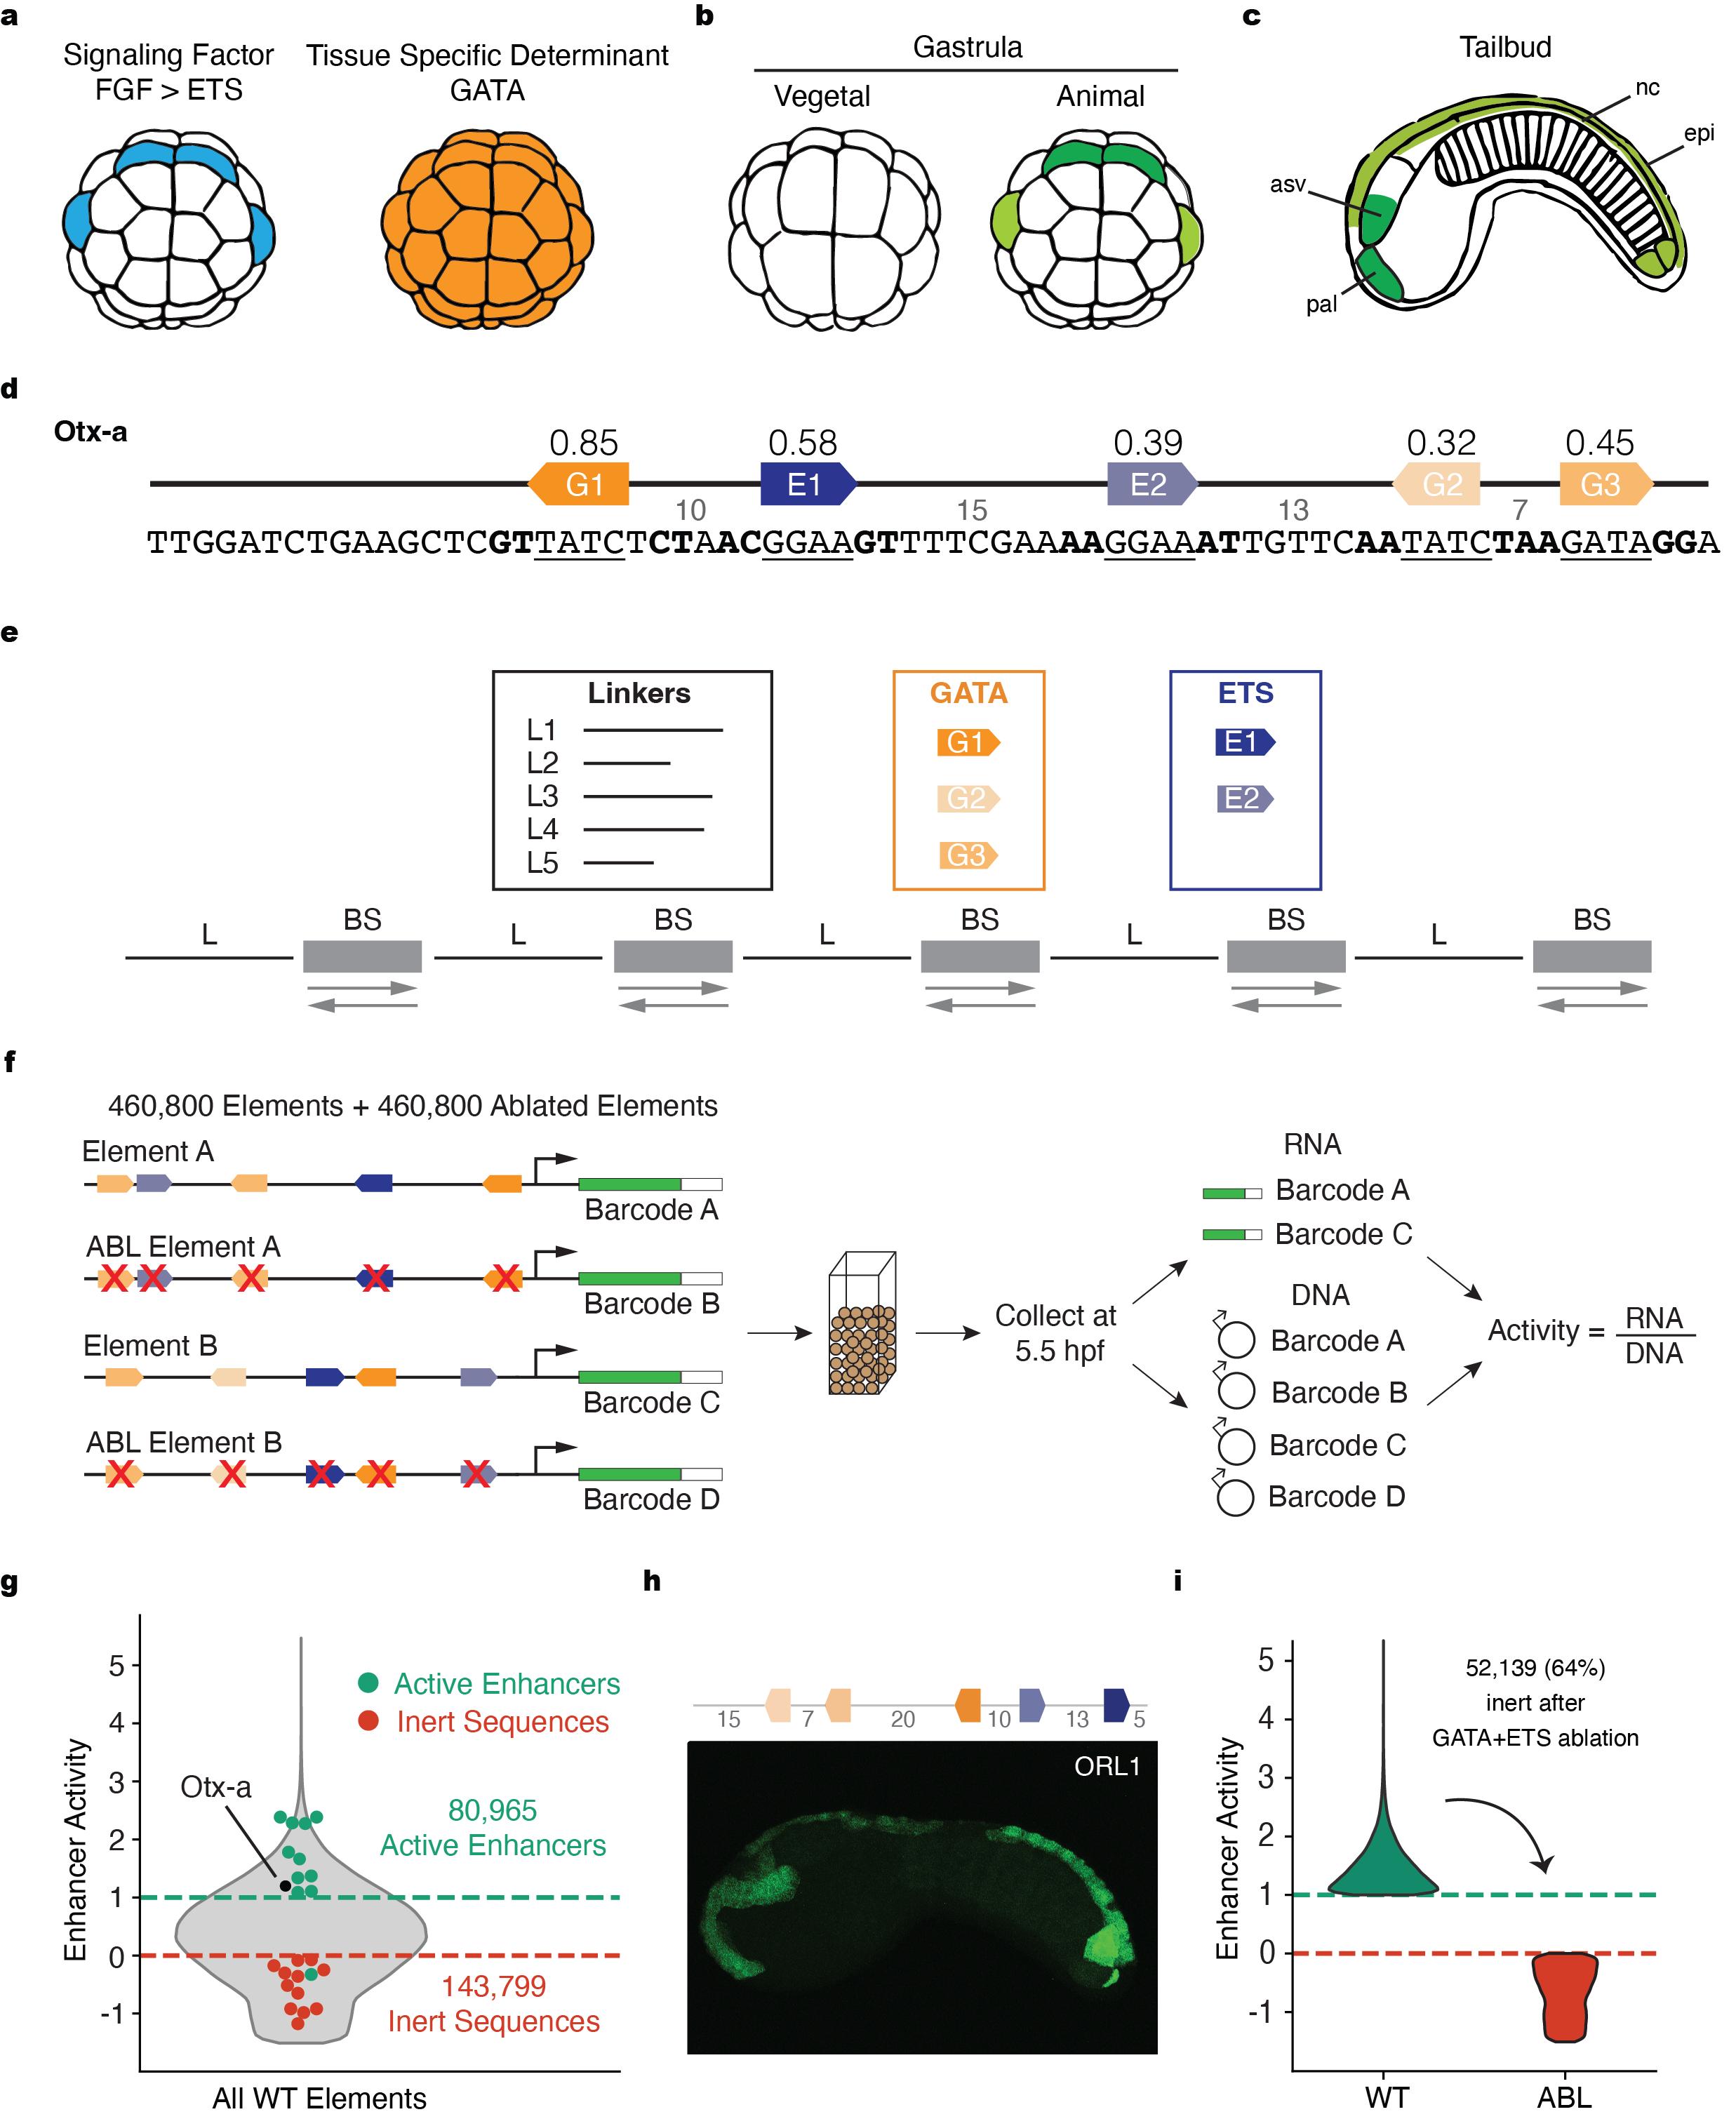
\includegraphics[height=0.8\textheight, keepaspectratio]{2_figures-and-files/Fig1.png}
    \caption[Screening every possible rearrangement of TFBSs in the \textit{Otx-a} enhancer via MPRA.]{\textbf{Screening every possible rearrangement of TFBSs in the \textit{Otx-a} enhancer via MPRA}.}
    \label{fig:2 Figure 1}
\end{figure}

\clearpage

%%%%%%%%%%%%%%%%%%%%%%%%%%%%%%%%%%%%%%%%%%%%%%%%%%%%%%%%%%%%%%%%%%%%%%%%%%%%%%%%

\subsection{TFBS syntax alone accurately predicts enhancer activity}

We next sought to build an accurate classifier of the functional enhancers in this screen. We reasoned that the 52,139 functional enhancers dependent on GATA and ETS should be predictable from the syntax of the five TFBS alone and developed a simple encoding of sequences that captures only the type, orientation and position of each TFBS core (\textbf{Figure~\ref{fig:2 Figure 2}a}, see Methods). This “syntax encoding” allows the model to flexibly learn combinations of TFBS that drive activity without having to hand-craft these features \textit{a priori}. It also eliminates the influence of any features in the linker sequences or at junctions that we do not expect to be major drivers of enhancer function in this screen.

We generated training and test data such that no two syntaxes appeared in both sets and evaluated several types of neural network classifiers that utilized the syntax encoding (\textbf{Figure~\ref{fig:2 Figure 2}b}). A convolutional neural network (CNN) with dilated convolutions and residual connections\cite{Koo2021-ly} performed best across 10-folds of cross validation (\textbf{Supplementary Figure~\ref{fig:2 supplementary_6}}), and achieved an area under the precision-recall curve (auPRC) of 0.59 on held-out test data (\textbf{Figure~\ref{fig:2 Figure 2}c}). We call this model Sirius in homage to its canine-named predecessors\cite{Kelley2016-oh,Gosai2023-cw}.

We found that Sirius’s performance was not dependent on using only active enhancers driven by GATA and ETS and that including the full set of 80,965 active enhancers as positives led to almost identical predictions and performance (\textbf{Supplementary Figure~\ref{fig:2 supplementary_7}}). Including affinity (\textbf{Figure~\ref{fig:2 Figure 2}c}, Sirius + Affinity) led to only a marginal increase in performance, indicating that placement of sites with differing affinities plays a relatively small role in this screen compared to syntax. We also evaluated Sirius’s ability to predict the continuous MPRA activity level using the raw scores produced by the model (see Methods). Despite being trained on binary labels, we found a modest correlation with activity level (\textbf{Supplementary Figure~\ref{fig:2 supplementary_7}}). Surprisingly, training models to directly predict continuous activity levels from all detected sequences in a regression setting yielded comparable performance (\textbf{Supplementary Figure~\ref{fig:2 supplementary_7}}). 

We designed the syntax encoding to ensure the spurious features are ignored by the model, but it is possible that the linear DNA sequence contains bona fide learnable features (e.g., flanks or de novo sites). We therefore benchmarked sequence-based models on the same task (\textbf{Figure~\ref{fig:2 Figure 2}c}, \textbf{Supplementary Figure~\ref{fig:2 supplementary_8}a}, \textbf{Supplementary Figure~\ref{fig:2 supplementary_8}b})\cite{Ghandi2014-ql}. A model trained on sequence of the same architecture (SiriusSeq) outperformed Sirius, but the relatively small improvement highlights that most of the information needed to predict activity is present in the TFBS cores. The performance of SiriusSeq was only slightly higher than Sirius + Affinity, suggesting that the additional predictive information in the sequence comes from the flanks. To directly test which sequence features SiriusSeq prioritized, we evaluated test set performance on sequences in which we randomized different features (\textbf{Figure~\ref{fig:2 Figure 2}d}, \textbf{Supplementary Figure~\ref{fig:2 supplementary_8}c}). We observed that the randomization of linker sequences led to a drop in predictive accuracy of similar magnitude to randomization of TFBS cores. Motif enrichment analysis from model-derived features (see Methods) pinpointed several motifs resembling sites with flanking nucleotides, and did not detect any known de novo motifs (\textbf{Supplementary Figure~\ref{fig:2 supplementary_8}d}, \textbf{Supplementary Table 2}). Taken together, these results suggest that syntax alone is enough to build an accurate and robust predictor of enhancer function from this screen, and that the additional information present in flanks and linkers has a relatively small contribution to enhancer function.

\clearpage

\thispagestyle{plain}
\noindent
\textbf{Figure~\ref{fig:2 Figure 2}. A convolutional neural network trained on TFBS syntax accurately discriminates inert sequences from active enhancers}. a) Syntax encoding schematic. Each library member is encoded by the position of GATA and ETS sites in both forward and reverse orientations, capturing order, orientation and spacing of the sites (see Methods). b) Machine learning model training schematic. Library members are partitioned into training, validation and test sets (see Methods). Training sequences are syntax encoded and used to train neural networks. Model predictions are continuous values that are transformed to probabilities via the sigmoid function and compared to MPRA labels to assess classification performance. c) Precision-recall curves for syntax encoding (Sirius), syntax + affinity encoding (Sirius + Affinity) and sequence (SiriusSeq) on held-out test data. Area under the curve (auPRCs) are indicated in parentheses. The dashed grey line indicates the performance of a random classifier. d) SiriusSeq held-out test set auPRCs on sequences with the indicated randomized features.

\clearpage

\begin{figure}[!htbp]
    \centering
    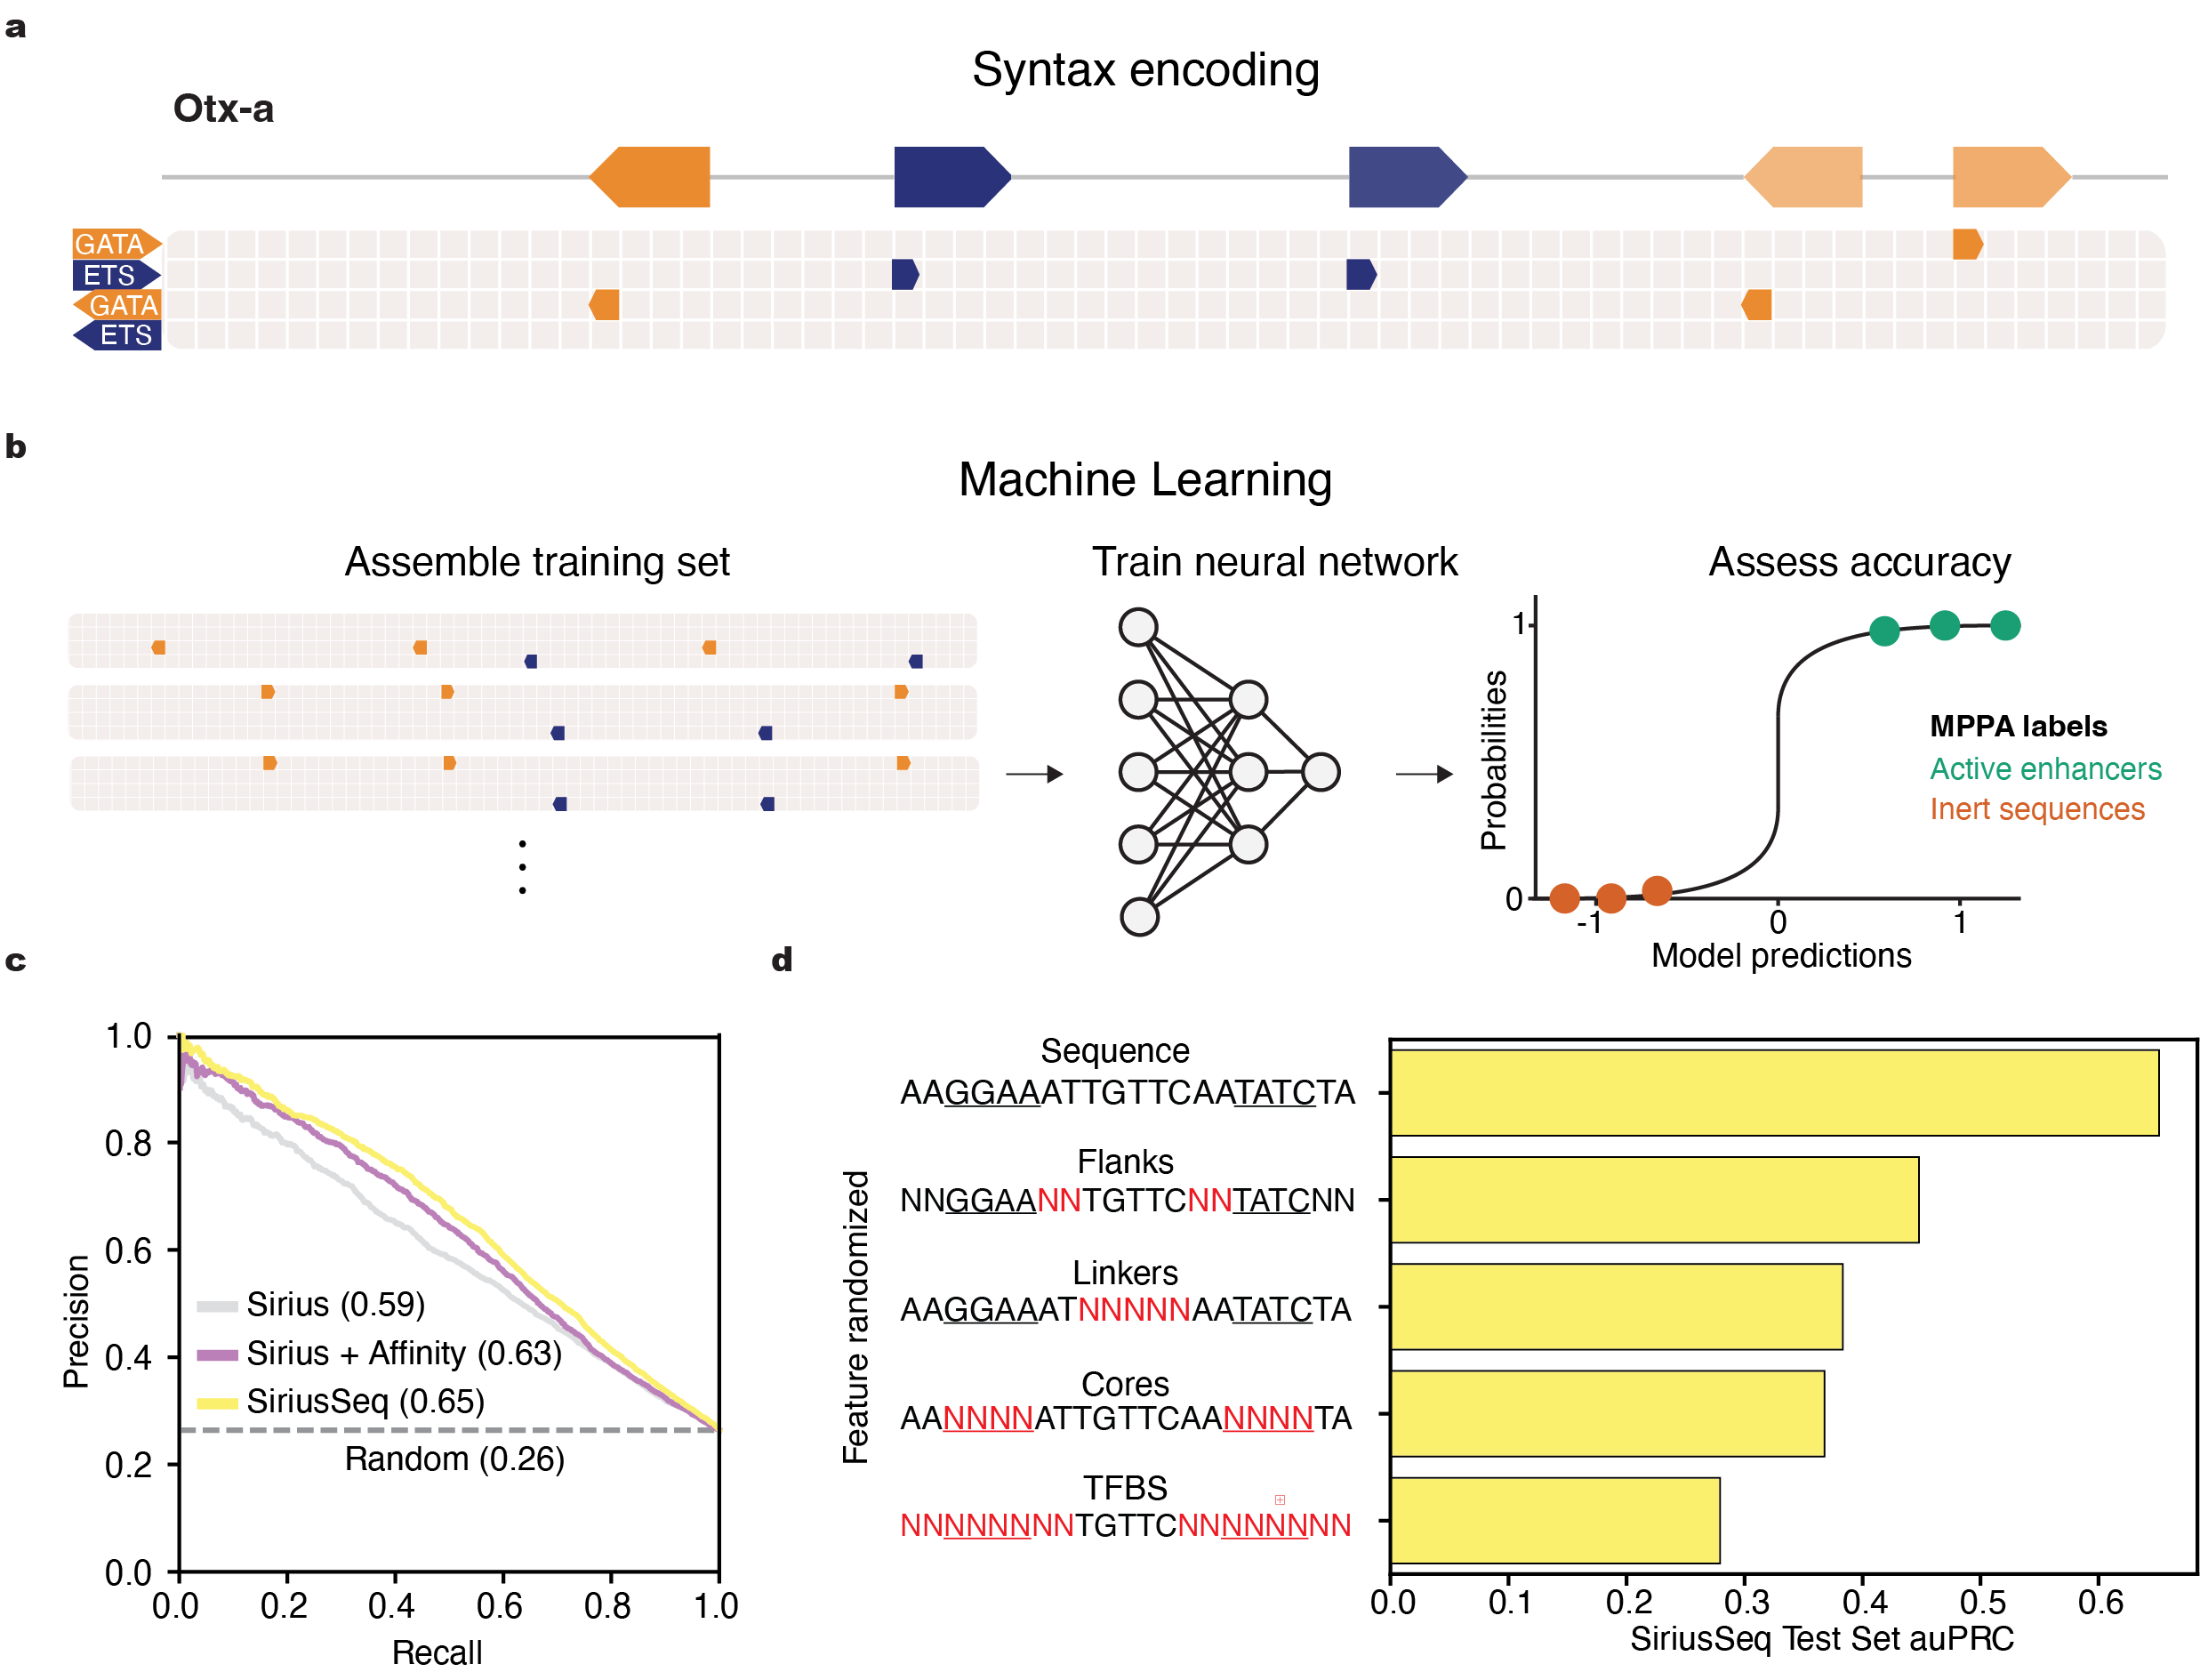
\includegraphics[height=0.7\textheight, keepaspectratio]{2_figures-and-files/Fig2.png}
    \caption[A convolutional neural network trained on TFBS syntax accurately discriminates inert sequences from active enhancers.]{\textbf{A convolutional neural network trained on TFBS syntax accurately discriminates inert sequences from active enhancers}.}
    \label{fig:2 Figure 2}
\end{figure}

\clearpage

%%%%%%%%%%%%%%%%%%%%%%%%%%%%%%%%%%%%%%%%%%%%%%%%%%%%%%%%%%%%%%%%%%%%%%%%%%%%%%%%

\subsection{Sirius learns a primarily additive model of TFBS syntax features}

Identification of TFBS syntax rules that govern enhancer function remains a central challenge in regulatory genomics\cite{Jindal2021-zk}. Although neural networks are often viewed as black boxes, methods for interpreting trained models can reveal the sequence features they prioritize and help us better understand how they arrive at their predictions\cite{Novakovsky2022-ft}. To investigate the most significant features in our screen, we systematically analyzed patterns of two and three binding sites, referred to here as organizational features (see Methods), and measured their impact on model predictions by marginalizing them across all the syntaxes they occurred in (\textbf{Figure~\ref{fig:2 Figure 3}a}). This yielded 15 significantly inactivating and 23 significantly activating 2-site features, as well as 654 inactivating and 1005 activating 3-site features (\textbf{Figure~\ref{fig:2 Figure 3}b}), which we refer to collectively as syntax features. We found that both activating 2-site and 3-site features were enriched for configurations containing two ETS sites (\textbf{Supplementary Figure~\ref{fig:2 supplementary_9}a}), highlighting the importance of the proper configuration of ETS sites in functional syntaxes. Activating syntax features preferentially occurred toward the downstream half of the 66bp sequence, while inactivating features showed a slight positional skew upstream (\textbf{Supplementary Figure~\ref{fig:2 supplementary_9}b}). Additionally, a subset of 2-site features exhibited periodic positional preferences, potentially reflecting helical phasing constraints or other spacing-related syntax rules (\textbf{Supplementary Figure~\ref{fig:2 supplementary_9}c}).

To validate predicted syntax features, we first experimentally tested two in which we observed strong predicted activating effects. We synthesized sequences containing only a single instance of each syntax feature and assayed their activity \textit{in vivo} using fluorescence microscopy. Both sequences drove \textit{Otx-a} WT like expression, consistent with their predicted activating function (\textbf{Figure~\ref{fig:2 Figure 3}c}). We also observed several instances where subtle changes in 3-site syntax features create opposite directions of effect (\textbf{Supplementary Figure~\ref{fig:2 supplementary_9}d}). For instance, the organizational feature g.14.e.8.g is predicted to be an inactivating syntax feature (\textbf{Figure~\ref{fig:2 Figure 3}d}, left), but when the central ETS site is flipped to the forward strand, it is predicted to be activating (\textbf{Figure~\ref{fig:2 Figure 3}d}, right). Consistent with model predictions, a syntax containing the inactivating variant showed no activity, while the same syntax with only the ETS site flipped showed \textit{Otx-a} WT like expression (\textbf{Figure~\ref{fig:2 Figure 3}d}).

To better understand how the model combines the individual effects of syntax features to make its final prediction, we designed an additive model that sums the effect sizes of all organizational features present in a given sequence (\textbf{Figure~\ref{fig:2 Figure 3}e}, AdditiveFeatures). This additive model explained 56\% of the variance in the predictions made by Sirius (\textbf{Supplementary Figure~\ref{fig:2 supplementary_9}e}) and captures approximately 81\% of the gain in its predictive performance compared to a random classifier (\textbf{Figure~\ref{fig:2 Figure 3}f}). This suggests that a large portion of the model’s predictive capacity is driven by the independent contributions of individual syntax features it has learned to prioritize. While non-linear interactions between these features likely exist, they play a relatively minor role compared to linear ones.

\clearpage
\thispagestyle{plain}
\noindent
\textbf{Figure~\ref{fig:2 Figure 3}.} \textbf{Sirius combines syntax-features in a primarily additive model}. a) Schematic for organizational feature marginalization analysis. Each of 9,022 2-site and 3-site organizational features (see Methods) is tested by splitting up all 460,800 sequences in the library into those that do not contain the feature (No Feature) and those that do (Contains Feature). A Mann-Whitney U-test on the distribution of model predictions for the two groups is used to assign statistical significance (corrected with Benjamini-Hochberg method) and the relative log-odds of mean predictions between groups is used to define an effect size. b) Volcano plots for 2-site (left) and 3-site (right) syntax features where the x-axis shows log2 of the mean relative odds predicted by the model and the y-axis shows -log10(corrected p-value) from the Mann-Whitney U-Test in a). Organizational features are colored based on whether their adjusted p-value is < 0.01 and log2 relative odds is greater than 1 (activating, doubling of odds) or less than -1 (inactivating, halving of odds). c) Two 3-site syntax features that are predicted to be strongly activating act as synthetic active enhancers. d) A single strand flip of an ETS site in a 3-site syntax feature turns it from inactivating (left) to activating (right). e) Schematic for generating a AdditiveFeature score for the \textit{Otx-a} WT sequence (see Methods). The mean relative odds for each organizational feature contained in the sequence are summed. f) Test set precision-recall curves of AdditiveFeature model compared to full syntax model (Sirius) and random classifier. Numbers in parentheses indicate area under the precision-recall curve (auPRC).

\clearpage

\begin{figure}[!htbp]
    \centering
    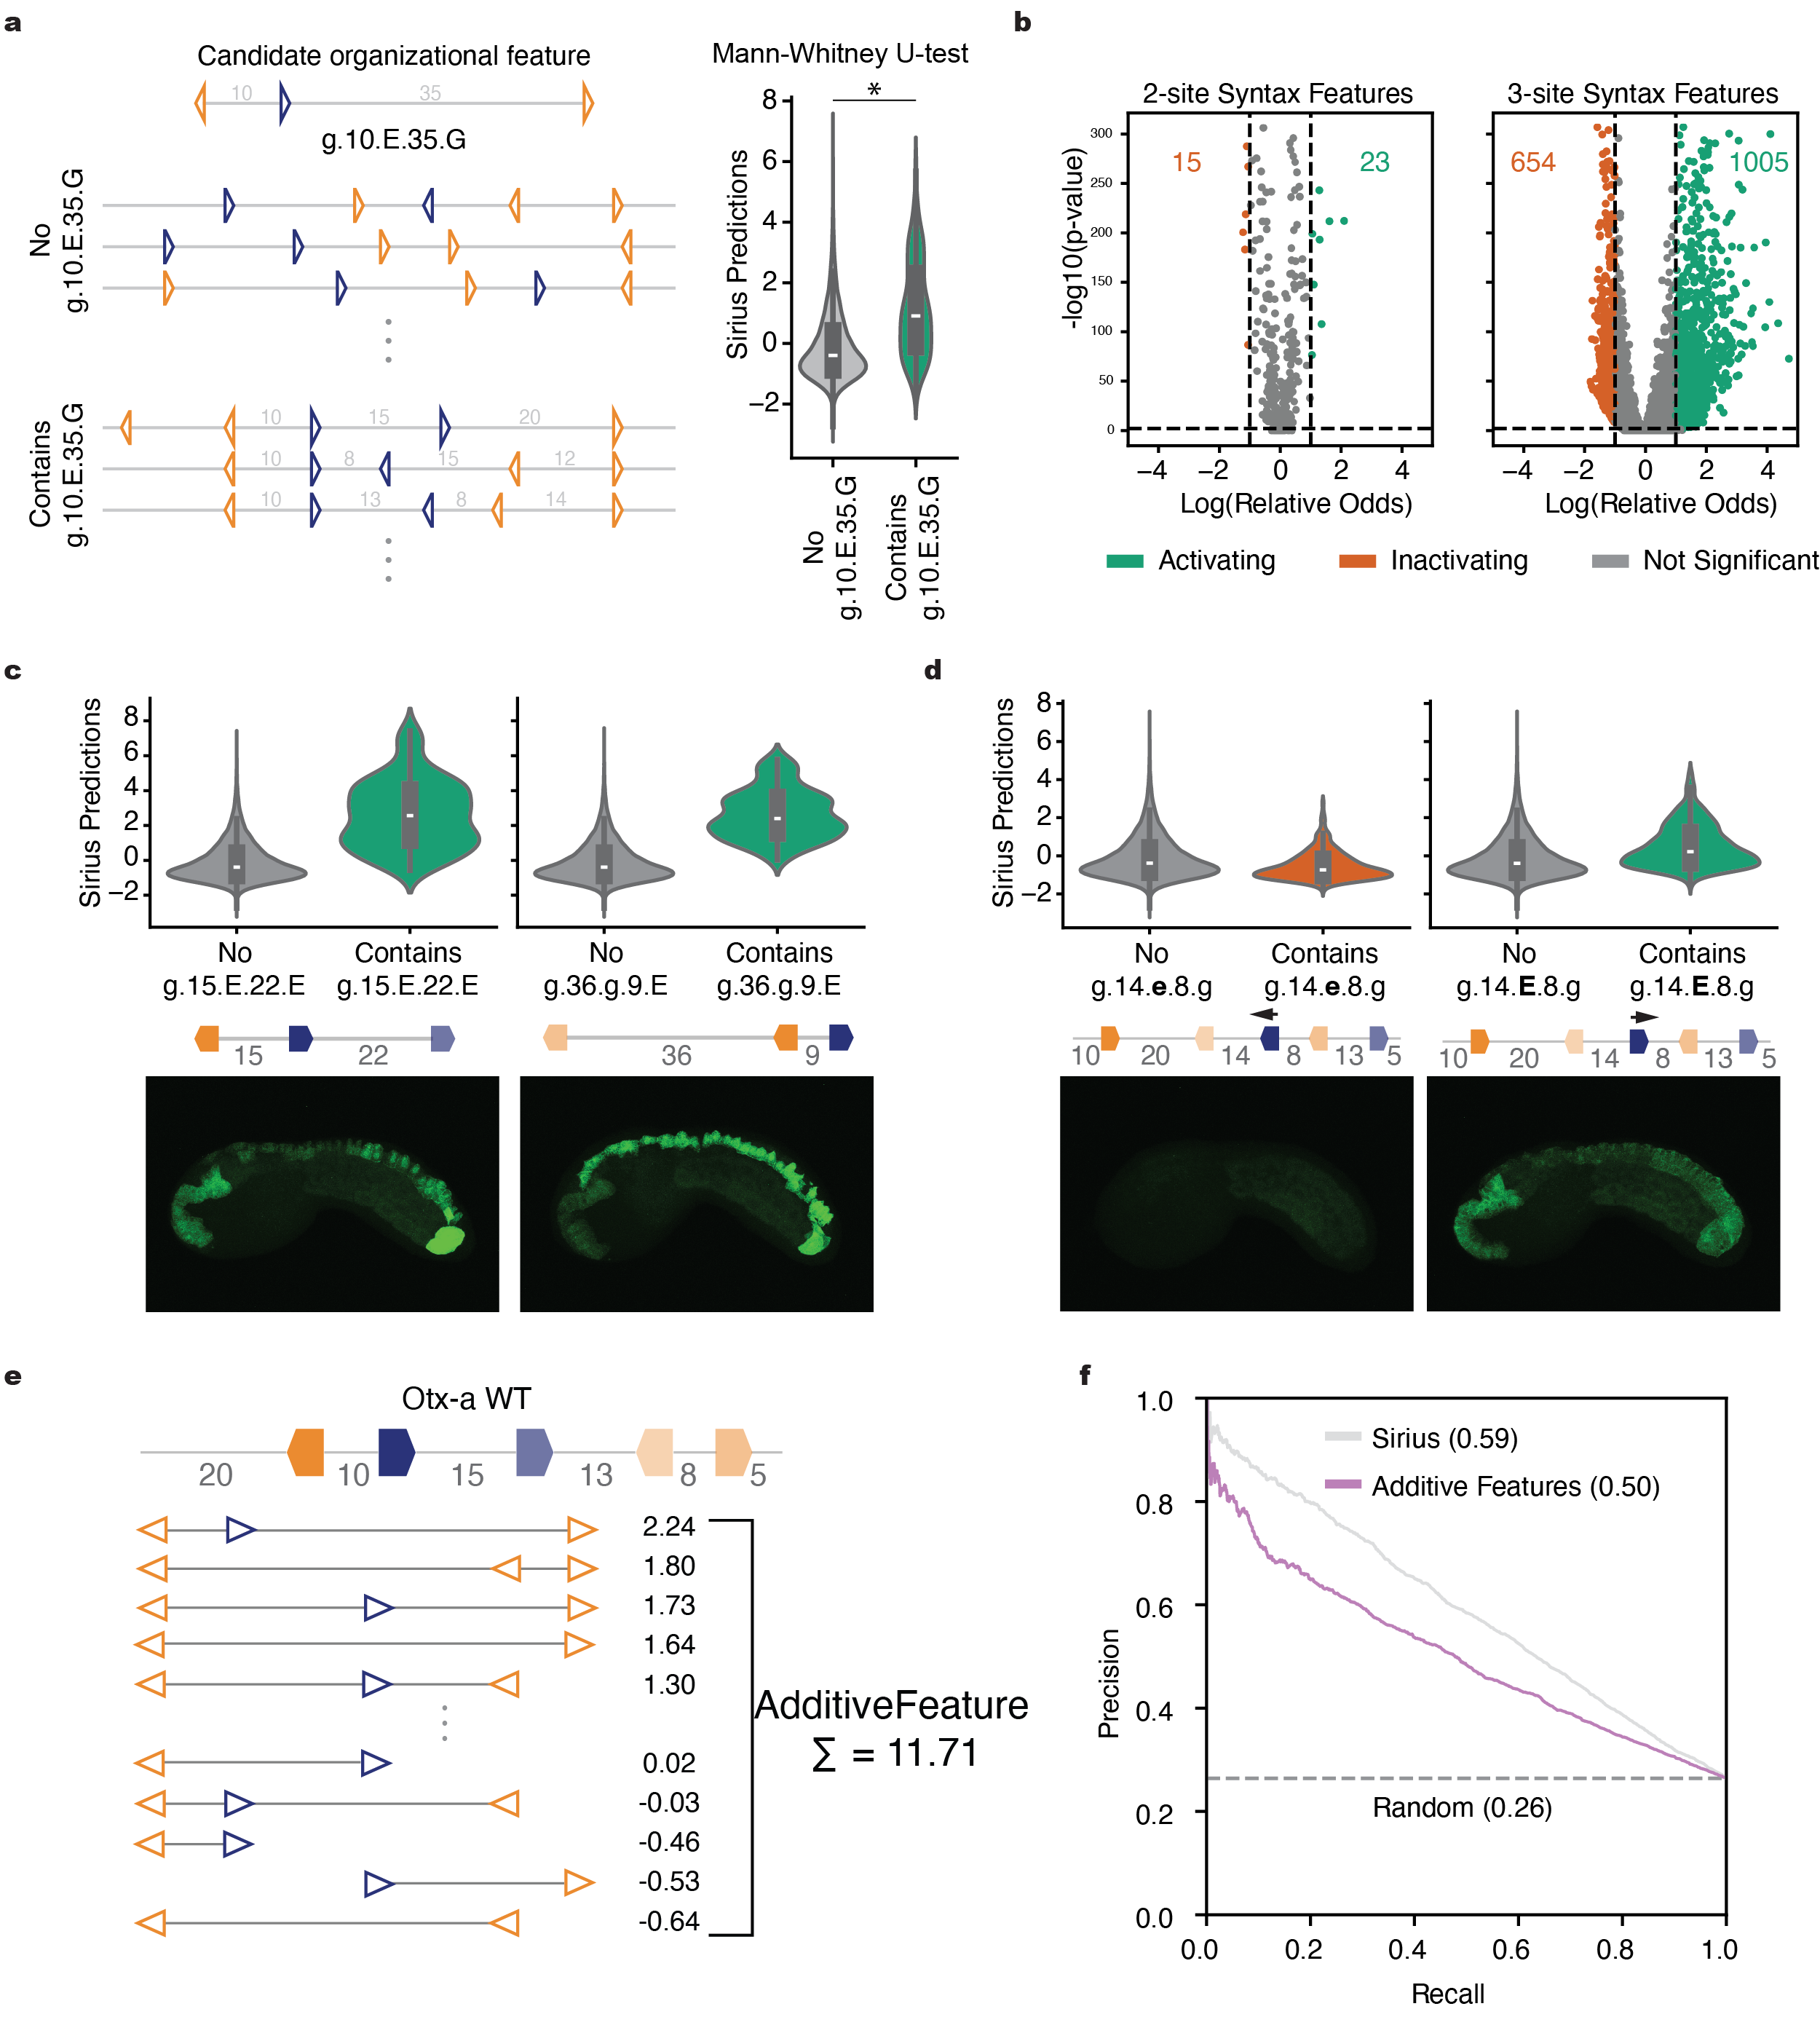
\includegraphics[height=0.75\textheight, keepaspectratio]{2_figures-and-files/Fig3.png}
    \caption[Sirius combines syntax-features in a primarily additive model.]{\textbf{Sirius combines syntax-features in a primarily additive model}.}
    \label{fig:2 Figure 3}
\end{figure}

\clearpage

%%%%%%%%%%%%%%%%%%%%%%%%%%%%%%%%%%%%%%%%%%%%%%%%%%%%%%%%%%%%%%%%%%%%%%%%%%%%%%%%

\subsection{Sirius enables tissue-specific enhancer design}

Of the sequences we validated using fluorescence microscopy, several showed activity in tissues other than the neural lineages expected for the WT \textit{Otx-a} enhancer (\textbf{Supplementary Figure~\ref{fig:2 supplementary_10}a}, \textbf{Supplementary Figure~\ref{fig:2 supplementary_10}b}). Sirius predictions for these “ectopic enhancers” were higher than those for neural-specific active enhancers (neural enhancers) (\textbf{Supplementary Figure~\ref{fig:2 supplementary_10}a}). To assess this more systematically, we categorized all the library sequences into three groups: 1) inert sequences, 2) neural enhancers and 3) ectopic enhancers, using a combination of MPRA activity and two other metrics previously shown to be predictive of tissue specificity. These three groups were well separated by Sirius predictions across models trained on different folds (\textbf{Supplementary Figure~\ref{fig:2 supplementary_10}c}, \textbf{Supplementary Figure~\ref{fig:2 supplementary_10}d}).

Inspired by previous work on synthetic enhancer design using neural networks\cite{Taskiran2023-xz,Gosai2023-cw}, we developed a strategy to design synthetic enhancers using Sirius (\textbf{Figure~\ref{fig:2 Figure 4}a}). The design process begins with a starting sequence for which we then select one of four possible “syntax edits” at random. A syntax edit is a perturbation made to the sequence that operates at the level of TFBS rather than the linear DNA sequence. Each type of syntax edit generates a set of candidate syntaxes, which we then score using a scoring function based on Sirius predictions, often the distance from a prespecified target value. Selecting the highest-scoring sequence from the pool of candidates generates a new starting point for another iteration of design. We continue this process for a set number of iterations or until a convergence threshold is reached. In this way, the model can be used to generate synthetic enhancers.

To test whether Sirius could design sequences with tissue specificity, we chose an objective function which minimizes the difference between Sirius predictions and the median of the neural enhancer group (\textbf{Supplementary Figure~\ref{fig:2 supplementary_10}c}). We call the sequences generated by this process STARS (Syntax-derived, Tissue-specific, Active Regulatory Sequences). We selected 16 starting syntaxes from our microscope-validated set to design neural enhancers from (\textbf{Supplementary Figure~\ref{fig:2 supplementary_10}b}), 14 are inert syntaxes that represent candidates for activating STARS and 2 are ectopic syntaxes that represent candidates for tuned STARS. For each starting syntax, we performed 25 rounds of design across multiple random seeds and selected STARS (see Methods). We generated single activated STARS from each of the 14 starting inert sequences (\textbf{Figure~\ref{fig:2 Figure 4}b}, \textbf{Supplementary Figure~\ref{fig:2 supplementary_11}a}) and five tuned STARS for each of the two starting ectopic sequences (tuned STARS) (\textbf{Figure~\ref{fig:2 Figure 4}c}, \textbf{Supplementary Figure~\ref{fig:2 supplementary_11}b}).

We then generated a library of sequences based on these 24 total STARS to experimentally validate via MPRA. For each of the STARS, we generated a total of 8 sequences by varying the composition of the flanks and linkers between the sites (\textbf{Supplementary Figure~\ref{fig:2 supplementary_12}}, see Methods). The final STARS library contained 421 unique sequences: 192 synthetic designs, a set of 192 ablated controls for each design, and 37 sequences from the OSL library controls. We split the sequences into two libraries to improve the signal to noise ratio, keeping the same set of 37 controls in each library. 

We electroporated both libraries into \textit{Ciona} embryos and quantified enhancer activity using the ratio of detected RNA barcodes to plasmid copy number for each sequence. Replicate concordance was high across the controls shared between libraries (\textbf{Supplementary Figure~\ref{fig:2 supplementary_13}a}). We again used a set of microscope-validated controls to determine activity thresholds classifying sequences as inert sequences, neural enhancers or ectopic enhancers (\textbf{Supplementary Figure~\ref{fig:2 supplementary_13}b}, \textbf{Supplementary Figure~\ref{fig:2 supplementary_13}c}, see Methods). Nearly all ablated sequences were inactive (190/192), indicating that the syntax of GATA and ETS sites drives activity for the sequences in this library (\textbf{Supplementary Figure~\ref{fig:2 supplementary_13}b}, \textbf{Supplementary Figure~\ref{fig:2 supplementary_13}c}). Among the activated STARS, 92\% (103/112) showed increased activity relative to their starting syntax, with 67\% (75/112) classified as active enhancers and 71\% (53/75) of those further classified as neural enhancers (\textbf{Figure~\ref{fig:2 Figure 4}d}). For tuned STARS, 95\% (76/80) decreased in activity, with 90\% (72/80) classified as either inert sequences or neural enhancers and 50\% (36/72) of those as neural enhancers (\textbf{Figure~\ref{fig:2 Figure 4}e}). Finally, SiriusSeq predictions across the STARS libraries showed a moderate but statistically significant correlation with MPRA activity and enhancer class labels (\textbf{Supplementary Figure~\ref{fig:2 supplementary_14}}). In sum, these results demonstrate that a syntax-based design approach can be used to generate synthetic enhancers with tunable and tissue-specific activity.

\clearpage

\thispagestyle{plain}
\noindent
\textbf{Figure~\ref{fig:2 Figure 4}. Syntax-driven design of tissue-specific synthetic enhancers}. a) Schematic of design process. We define four types of syntax edit that each generate a set of candidate syntaxes to score with the model. In each round of design, a syntax edit type is selected at random and candidate syntaxes are generated. Activity is then predicted with Sirius and transformed to a score using a chosen objective function. The highest scoring syntax is then selected for the next round of editing. Examples of activated (b) and tuned (c) STARS. Left, binding site syntaxes of sequences at each round. Right, model prediction for each round. Background colors are determined by the interquartile ranges of the Inert Sequence, Neural Enhancer and Ectopic Enhancer distributions shown in \textbf{Supplementary Figure~\ref{fig:2 supplementary_10}}c. STARS MPRA analysis for activated e) and tuned f) STARS. Y-axis shows change in measured activity of the designed sequence with respect to the measured activity of its starting sequence. Each syntax was used to generate eight different DNA sequences with differing flanks and linkers. Each point (sequence) is colored by the classification label assigned using thresholds from internal controls validated with fluorescence microscopy (\textbf{Supplementary Figure~\ref{fig:2 supplementary_13}}b,c). Barplot on top indicates the number of GATA and ETS sites in the respective designed syntax.

\clearpage

\begin{figure}[!htbp]
    \centering
    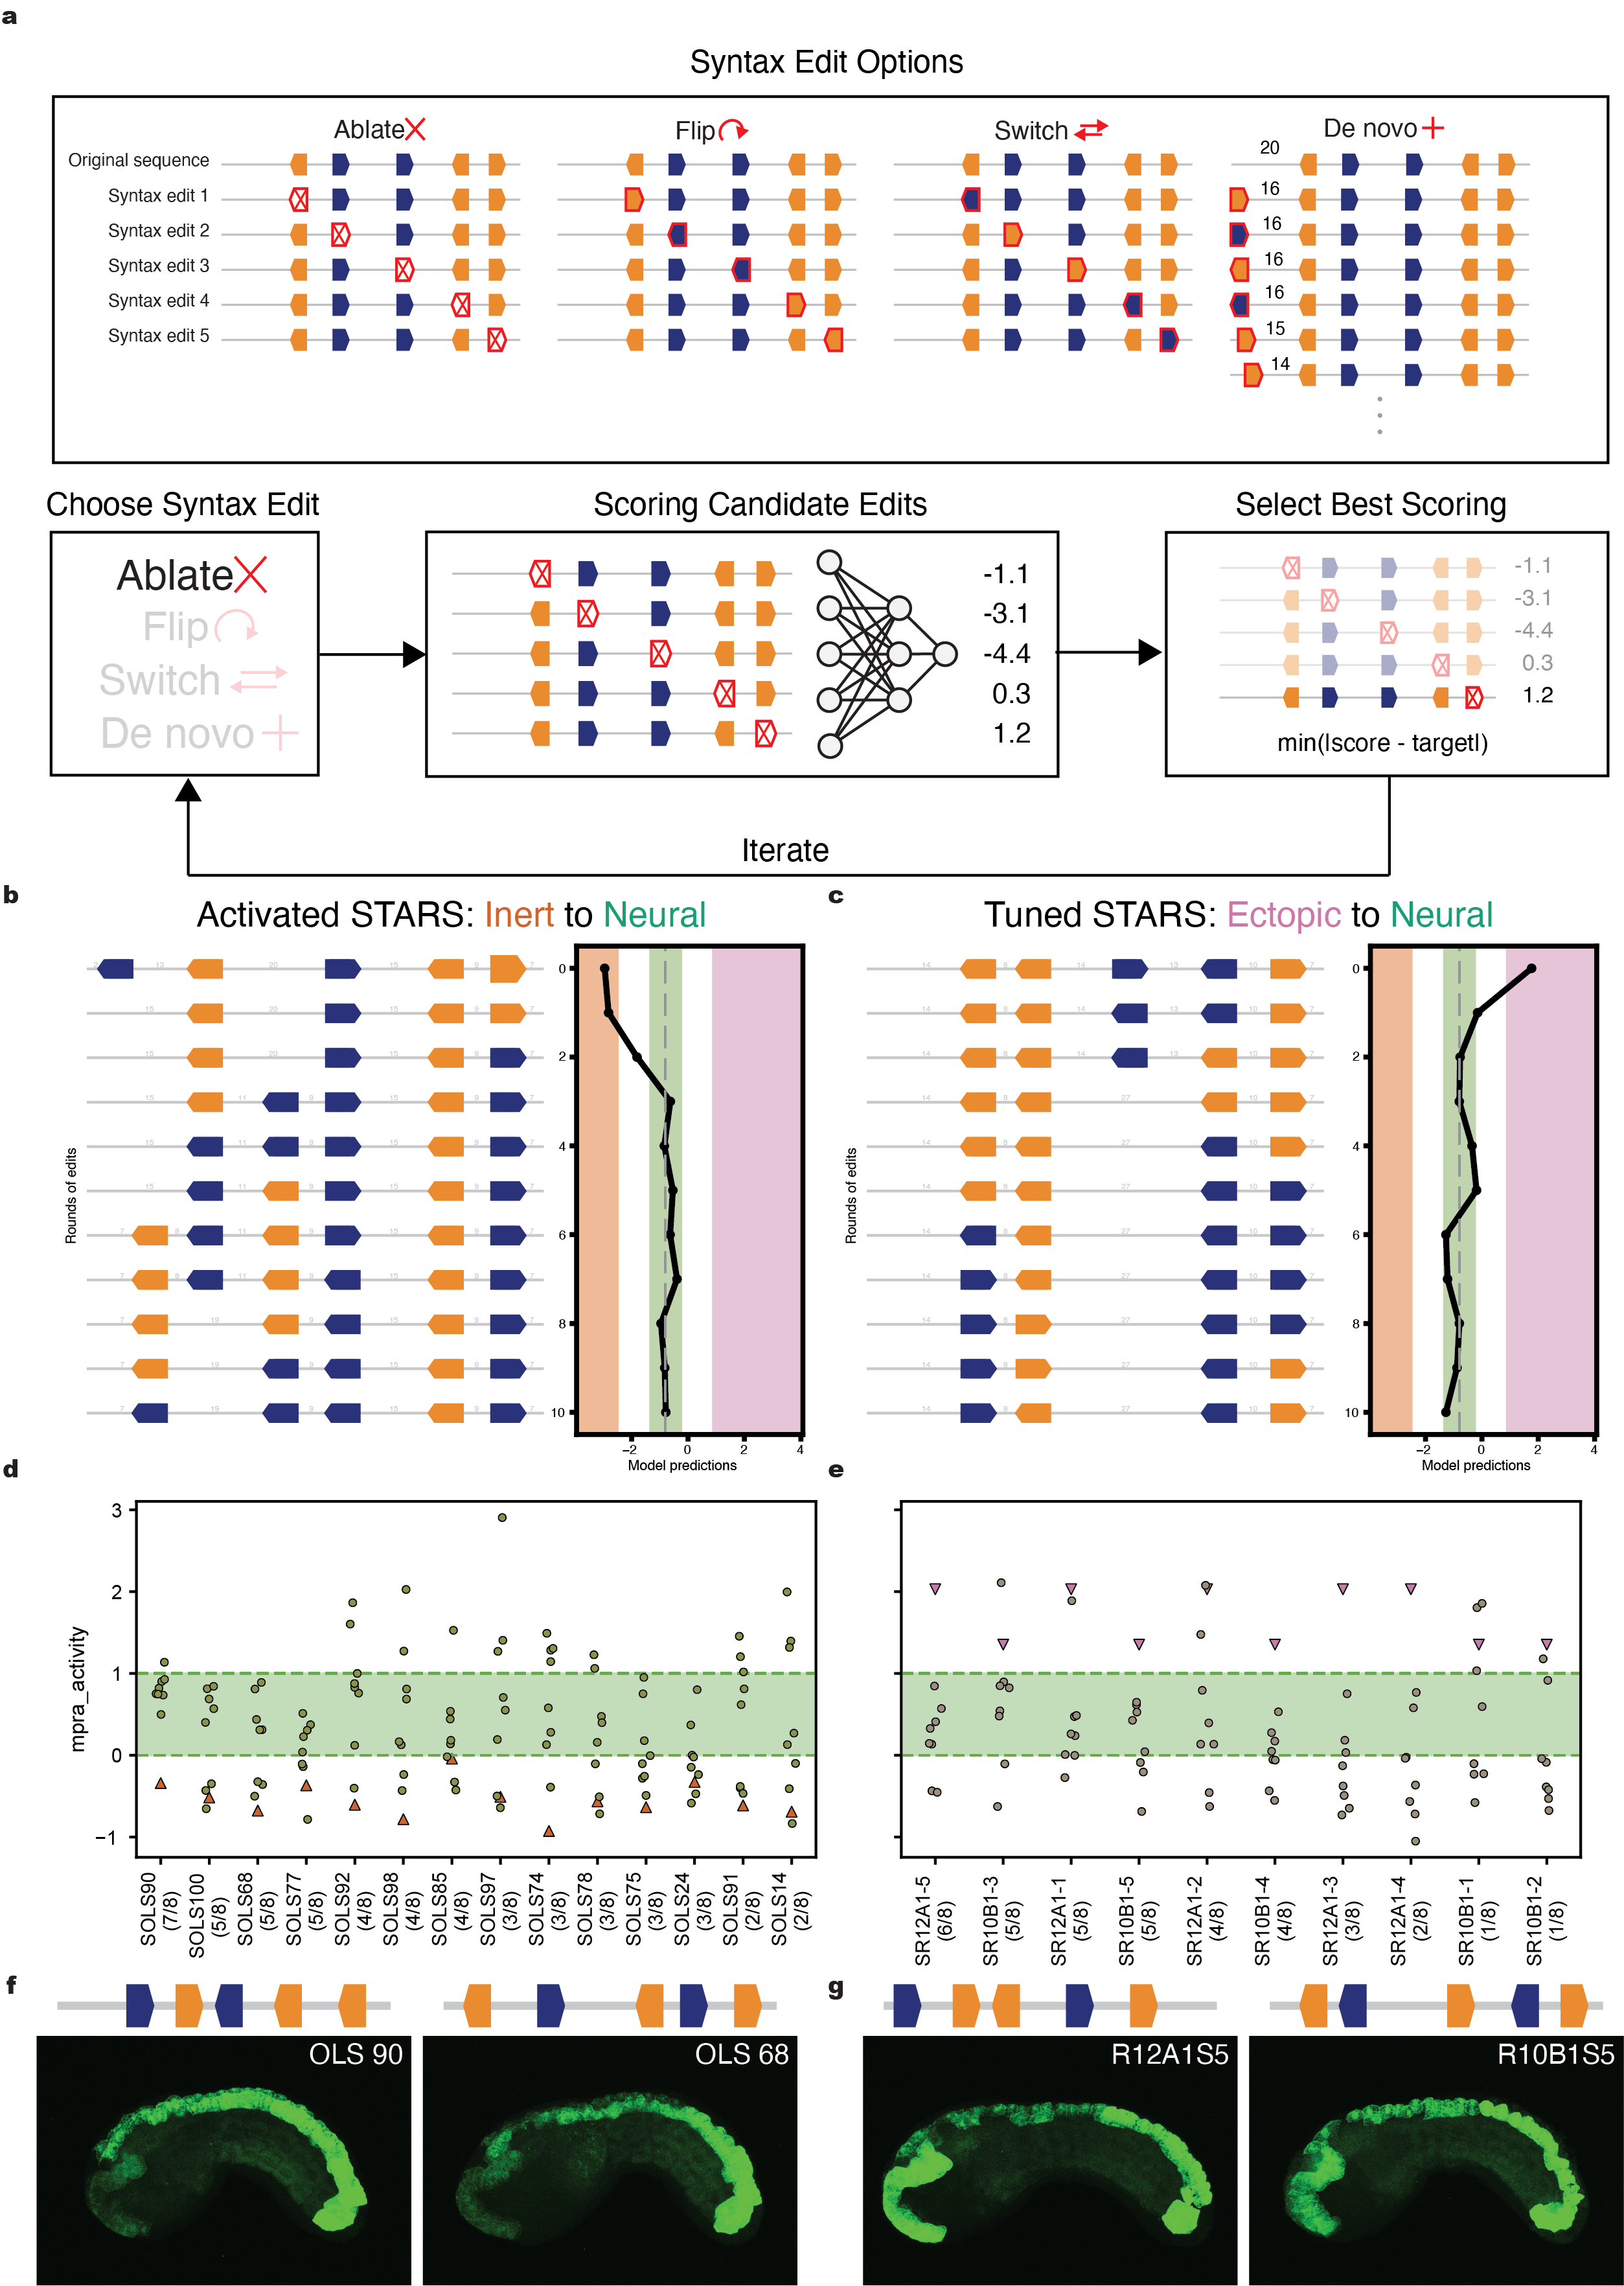
\includegraphics[height=0.75\textheight, keepaspectratio]{2_figures-and-files/Fig4.png}
    \caption[Syntax-driven design of tissue-specific enhancers.]{\textbf{Syntax-driven design of tissue-specific enhancers}.}
    \label{fig:2 Figure 4}
\end{figure}

\clearpage

%%%%%%%%%%%%%%%%%%%%%%%%%%%%%%%%%%%%%%%%%%%%%%%%%%%%%%%%%%%%%%%%%%%%%%%%%%%%%%%%

\subsection{Features beyond GATA/ETS syntax improve prediction of genomic enhancer function}

Clusters of ETS and GATA sites are widespread in the genome, but their regulatory potential is largely uncharacterized. We therefore created a sequence library from 66bp genomic elements that contain at least one ETS (>0.1 relative affinity), one GATA (>0.2 relative affinity) site, and a total of three or four sites (\textbf{Figure~\ref{fig:2 Figure 5}a}). This totaled 3,318 genomic elements, which we electroporated into \textit{Ciona} embryos and tested their activity via MPRA (\textbf{Figure~\ref{fig:2 Figure 5}b}, see Methods). We included six control sequences (including \textit{Otx-a} WT) with known expression patterns to establish thresholds for classifying active enhancers from inert sequences. We find that 1,148 of the genomic elements drive expression with levels similar to or greater than \textit{Otx-a} WT, and that 1,840 are inert (\textbf{Figure~\ref{fig:2 Figure 5}b}). The remaining 330 elements show very weak enhancer activity.

We first asked whether individual features could distinguish active enhancers from inert genomic sequences. Neither the number of sites (\textbf{Supplementary Figure~\ref{fig:2 supplementary_15}a}) nor the affinity of ETS sites (\textbf{Supplementary Figure~\ref{fig:2 supplementary_15}b}) differed significantly between active enhancers and inert sequences. In contrast, active enhancers tended to have modestly higher GATA site affinity than inert sequences (\textbf{Supplementary Figure~\ref{fig:2 supplementary_15}c}). Models trained on the OSL library showed only modest performance gains over a random classifier (auPRC = 0.38), of which Sirius was the highest (auPRC = 0.44) (\textbf{Figure~\ref{fig:2 Figure 5}d}). When stratified by aggregated affinity for each type of site, we observed an increase in the percentage of active enhancers for elements with strong syntax (top 20th percentile of Sirius predictions) relative to elements without syntax (bottom 20th percentile of Sirius predictions) (\textbf{Figure~\ref{fig:2 Figure 5}d}). We noted the strongest increase in three particular bins: 1) elements with high ETS affinity and low GATA affinity, 2) elements with high ETS affinity and high GATA affinity, and 3) elements with low ETS affinity bins and moderate GATA affinity.

The relatively modest predictive capability of these OSL trained models suggests that predictive features outside of those contained in the OSL library are present in the tested genomic clusters. Indeed, models trained directly on genomic sequences (Genomic Sequence) performed better than Sirius (\textbf{Supplementary Figure~\ref{fig:2 supplementary_15}d}), albeit with large variability across three folds, likely due to the sample size. We found that fine-tuning models trained first on the OSL library led to more reproducible performance, at the cost of some predictive power (\textbf{Supplementary Figure~\ref{fig:2 supplementary_15}d}). Fine-tuned sequence models had the highest mean test set performance across three folds (\textbf{Supplementary Figure~\ref{fig:2 supplementary_15}d}), with fine-tuned syntax and syntax + affinity models showing lower overall performance, but similar performance to each other.

To test whether our approach to modeling enhancer function based on TFBS syntax is generalizable beyond the \textit{Ciona} system, we analyzed data from a study of four core pluripotency transcription factors: Oct4, Sox2, Klf4, and Esrrb in mouse embryonic stem cells (mESCs)\cite{King2020-hk}. We first trained a Sirius-style model on a syntax encoding of the synthetic MPRA conducted in that study, achieving accurate quantitative predictions (R\textsuperscript{2} = 0.92) and a 6\% increase in performance over the published random forest model (R\textsuperscript{2} = 0.87) trained on hand-crafted features (\textbf{Supplementary Figure~\ref{fig:2 supplementary_16}a}). We also trained a Syntax + Affinity model on the genomic MPRA performed in the same study and achieved performance (auPRC = 0.82) exceeding the published gkm-SVM trained DNA sequence (auPRC = 0.77) (\textbf{Supplementary Figure~\ref{fig:2 supplementary_16}b}).

\clearpage

\thispagestyle{plain}
\noindent
\textbf{Figure~\ref{fig:2 Figure 5} OSL models predict activity of genomic clusters of ETS and GATA sites}. a) Schematic showing search for clusters of ETS and GATA binding sites. Each element contains at least one GATA site (relative affinity > 0.2) and one ETS site (relative affinity > 0.1). b) Enhancer activity of the 3,318 genomic elements tested in Ciona embryos. 1,148 elements are active enhancers while 1,840 elements are inert sequences. Activity of six internal controls are shown as the colored points: \textit{Otx-a} (black), three positive controls (green), and two negative controls (red). c) Precision-recall curves for OSL trained models on genomic clusters: Syntax encoding (Sirius), syntax + affinity encoding (Sirius + Affinity) and sequence (SiriusSeq). Areas under the curve (auPRCs) are indicated in parentheses. The dashed grey line indicates the performance of a random classifier. d) Percent of active enhancers within each group separated based on affinity and syntax. Each element is placed in a bin based on the summed affinity of ETS (heatmap Y-axis), summed affinity of GATA (heatmap X-axis) and the syntax group. Top heatmap contains elements with in the bottom 20th percentile of Sirius scores. Lower heatmap contains the elements in the top 20th percentile of Sirius scores.

\clearpage

\begin{figure}[p]
    \centering
    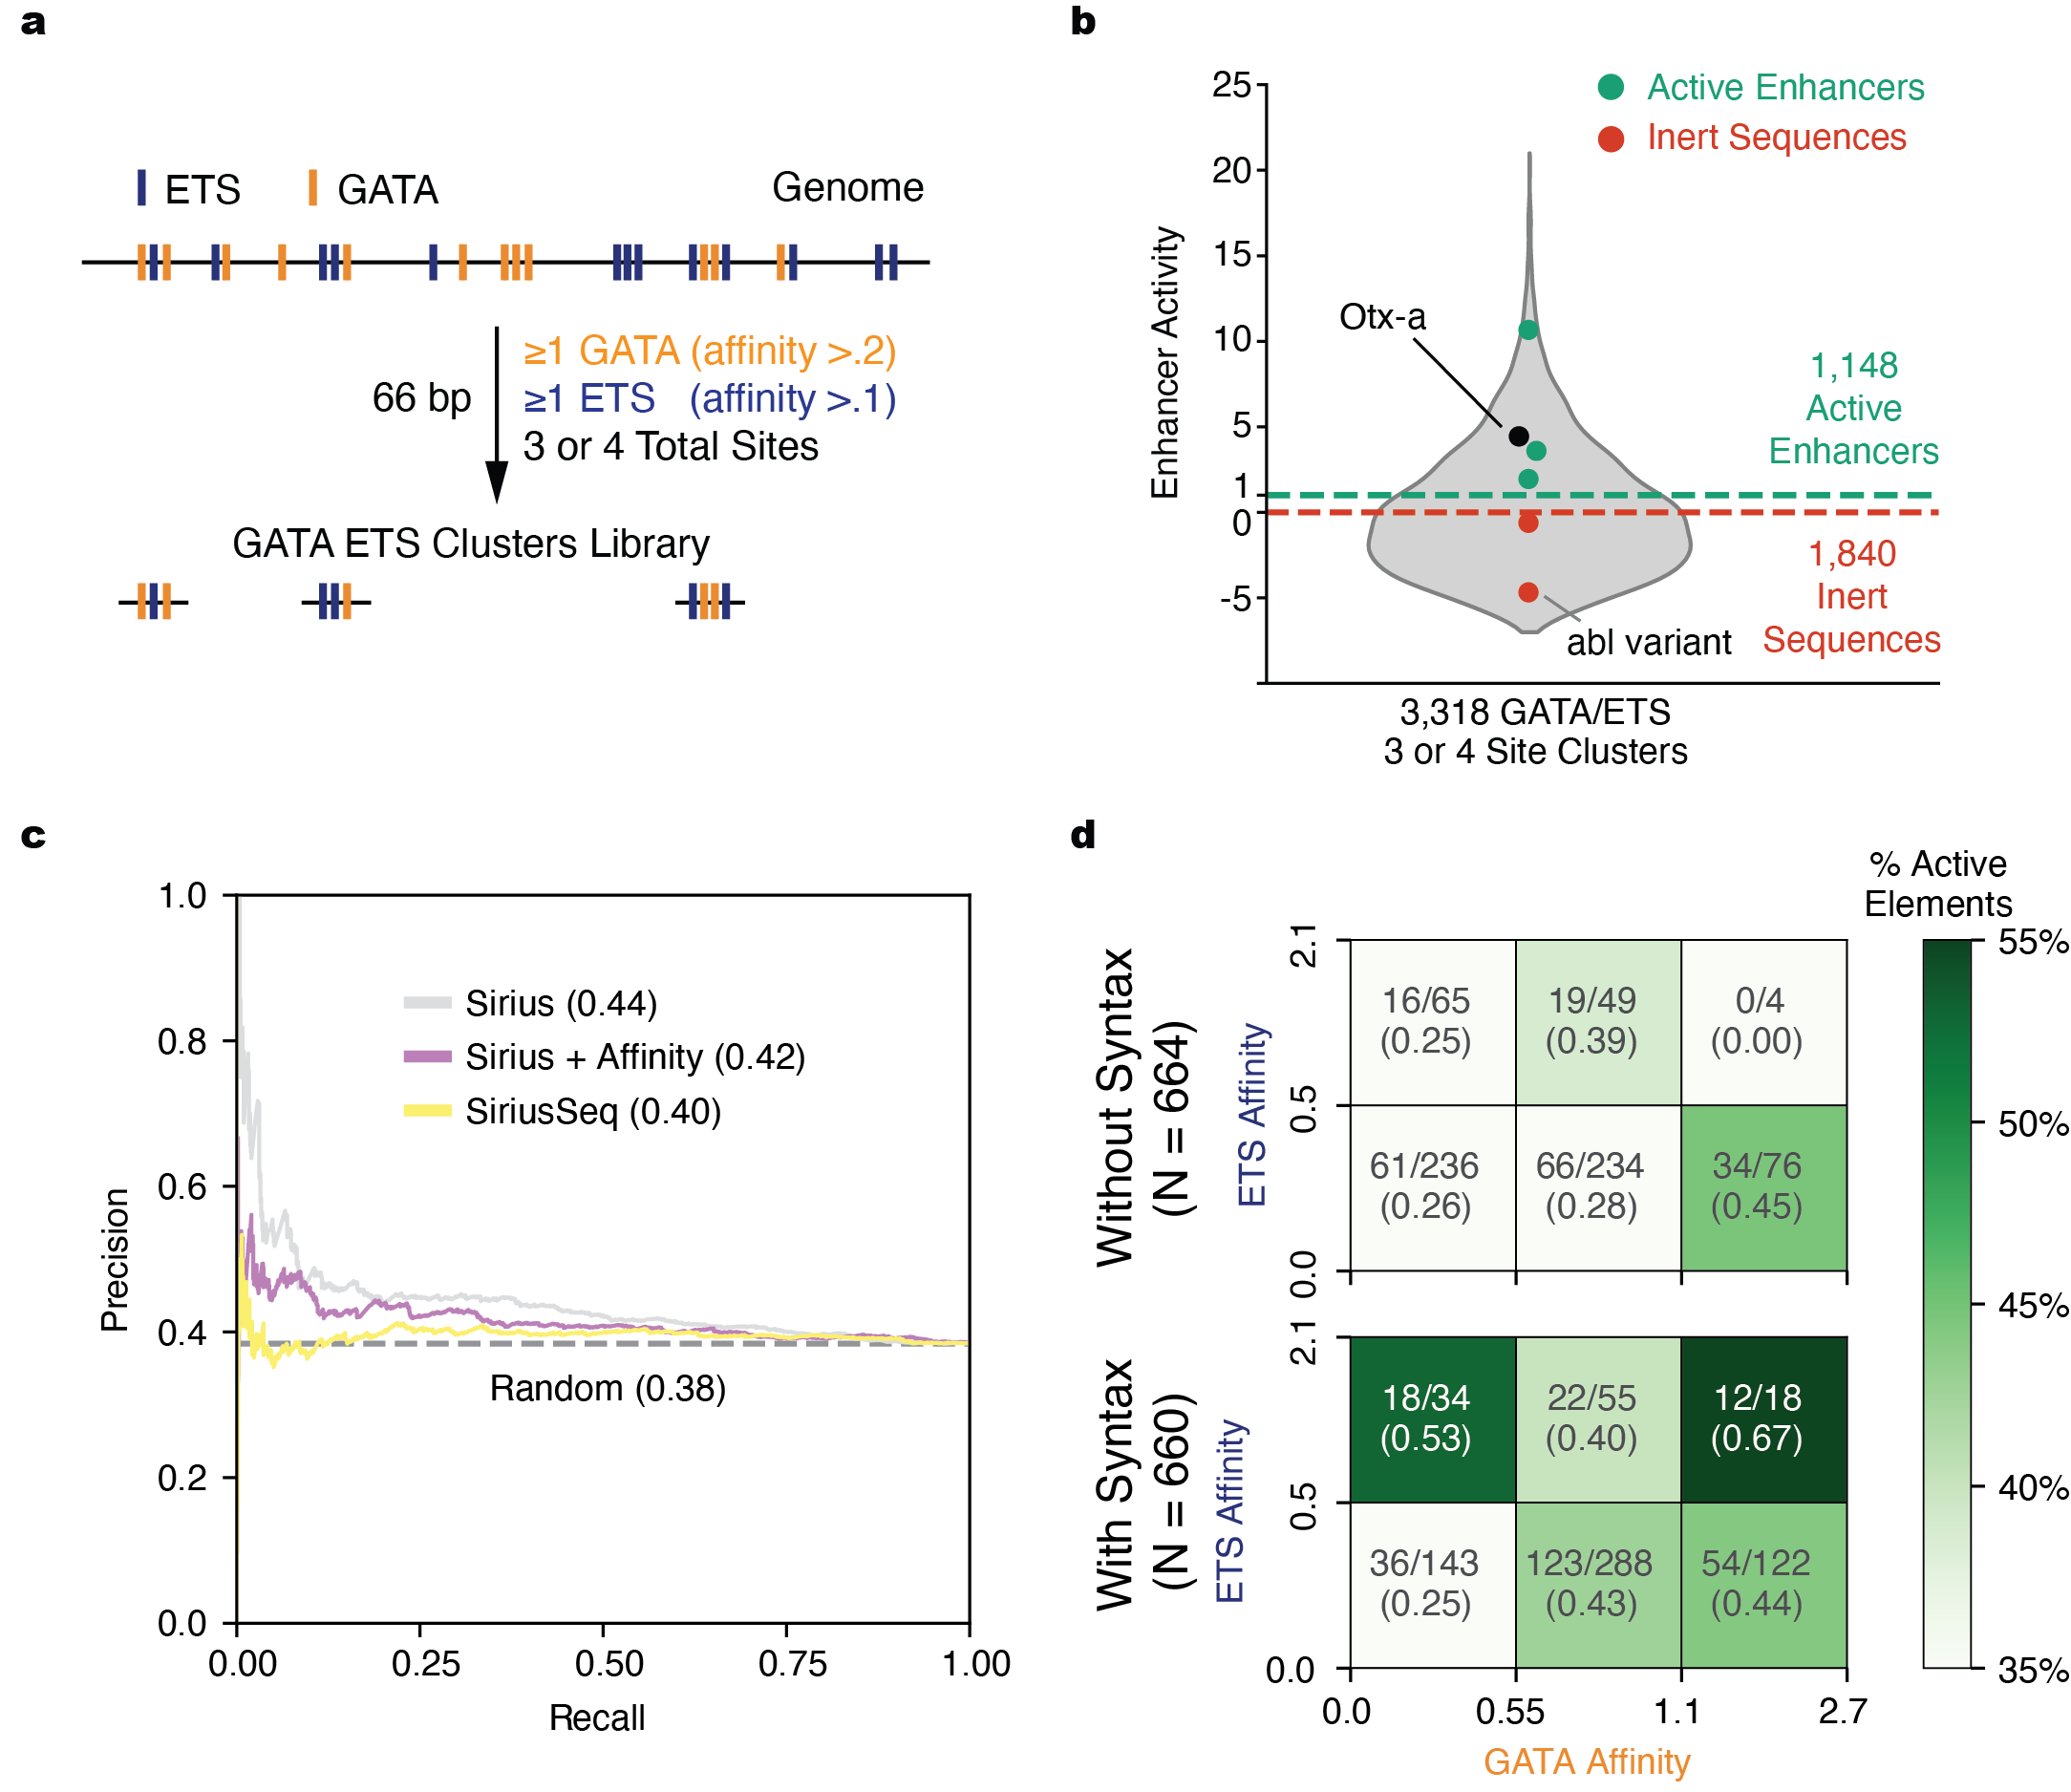
\includegraphics[height=0.7\textheight, keepaspectratio]{2_figures-and-files/Fig5.png}
    \caption[OSL models predict activity of genomic clusters of ETS and GATA sites.]{\textbf{OSL models predict activity of genomic clusters of ETS and GATA sites}.}
    \label{fig:2 Figure 5}
\end{figure}

\clearpage

%%%%%%%%%%%%%%%%%%%%%%%%%%%%%%%%%%%%%%%%%%%%%%%%%%%%%%%%%%%%%%%%%%%%%%%%%%%%%%%%
\section{Discussion}
%%%%%%%%%%%%%%%%%%%%%%%%%%%%%%%%%%%%%%%%%%%%%%%%%%%%%%%%%%%%%%%%%%%%%%%%%%%%%%%%

Years of work combining classical genetics, high-throughput genomic assays, and computational modeling have identified the number, identity, order, orientation, spacing, and affinity of TFBSs as key determinants of enhancer function \cite{Jindal2021-zk}. Yet despite this progress, our understanding of how sequence encodes function remains shallow. Here, we present a novel framework for learning how the sequence of an enhancer encodes function. By combining a deep profile of the grammar of a single enhancer with deep learning, we build an accurate model of enhancer function that successfully guides the design of tissue-specific synthetic enhancers.

The dataset generated in this study represents one of the most exhaustive and well-controlled investigations of enhancer syntax to date. By systematically permuting the order, orientation, and spacing of five experimentally validated TFBS, we created a library of over 900,000 synthetic sequences. Crucially, all elements in the library share the same TFBS identities, numbers, and affinities, allowing us to isolate the functional impact of syntax alone by eliminating confounding variables. When assayed in \textit{Ciona} embryos using MPRA, we found that the majority of TFBS combinations did not drive activity, underscoring the critical role of syntax in function. This result directly supports the idea that the \textit{Otx-a} enhancer is an enhancer that follows a dependency grammar\cite{Jindal2021-zk}, falling in between the enhancesome and billboard models.

A central goal in the study of enhancers is to predict their activity directly from DNA sequence. Most current approaches to this task use deep learning models trained on genomic data \cite{De-Winter2025-nz,Sasse2024-ly}, encoding the nucleotide sequence in an unbiased manner. While these models have proven powerful, disentangling the features they learn (e.g. TFBS identity, affinity, and syntax) and their impact on predictions is not always straightforward. Additionaly, extensive sequence homology in the genome renders them vulnerable to data leakage \cite{De_Boer2024-ic,Rafi2025-er}. Here, we take a complementary approach by representing each sequence in terms of the type, orientation, and position of TFBSs, and demonstrate that syntax alone is sufficient to accurately predict enhancer function in our screen. This approach also enables targeted comparisons of the effect of including specific features, illustrated by our comparisons of models trained on syntax, syntax and affinity, and sequence. Naturally, this approach depends on having prior knowledge of the TFBSs relevant for function and assumes that activity is driven primarily by those sites, which may not hold in more complex or less well-characterized systems. Still, in cases where these conditions are met, syntax-based models offer a powerful and generalizable framework for understanding and predicting enhancer function.

While our model performed well on the synthetic library, it only modestly generalized to the genomic context, as has been previously observed \cite{King2020-hk,Fromel2024-ux}. This suggests an opportunity to refine library designs by introducing greater variability in flanking and linker sequences while maintaining fixed TFBS content, or by using the model itself to design the next iteration of training data \cite{Friedman2023-yh}. Additional improvements may also come from improving the resolution of the synthetic MRPA, both in terms of signal-to-noise ratio and by incorporating tissue-specific readouts. Despite the limitations of the training data, elements with high Sirius scores were consistently enriched for active enhancers across a range of TFBS affinity levels, highlighting that syntax contributes additional predictive signal. These results suggest that syntax is a broadly useful feature for predicting enhancer function, but that it alone is usually insufficient to capture the full complexity of enhancer activity in the genome.

Although neural networks are often viewed as black boxes, model interpretation can help uncover the features they use to make predictions \cite{Novakovsky2022-ft}. In this work, we used a relatively simple marginalization strategy to identify combinations of two and three TFBSs that significantly contribute to enhancer activity and demonstrate that Sirius learns a primarily additive function of these features. This may reflect a billboard model at the level of syntax features rather than individual sites, where only an enhancer with a critical mass of activating syntax features is capable of recruiting a stable transcriptional complex and driving gene expression. Our approach, however, relies on exhaustively enumerating and marginalizing a fixed and tractable number feature combinations, a strategy that may not scale well or generalize to more complex systems. New interpretation methods tailored to syntax models could help uncover non-additive interactions or higher-order rules that are cannot be captured through our margainalization approach. Unsupervised methods in particular, such as clustering learned representations for each sequence, may aid the discovery of latent structure in enhancer grammar and whether that structure operates in distinct states, or along a continuous manifold.

Designing synthetic enhancers with predictable activity has important implications for both basic and translational genomics. Our work complements existing approaches that use large-scale genomic screens or chromatin accessibility data by showing that synthetic screen can be leveraged to design sequences with targeted regulatory activity. Nearly all of our designed enhancers showed tuned expression in the intended direction, and a substantial proportion exhibited MPRA activity consistent with neural-specific enhancers. Initially, we were surprised to find that, despite being trained on bulk data, Sirius could predict function with apparent tissue specificity. One possible explanation for this lies in the primarily additive model Sirius appears to learn. Sirius may be learning that increasing the number of activating syntax features in an enhancer makes it progressively easier to assemble a functional transcriptional complex and that when this assembly becomes too efficient, it will occur even in tissues with lower TF concentrations, leading to broader, less specific activity. This supports the idea that suboptimal syntax is a key determinant of tissue-specific enhancer function\cite{Farley2015-xx,Farley2016-eh}. Still, we assessed enhancer activity using bulk MPRA in this study, and tissue resolved data is ultimately needed to better evaluate Sirius, and to improve the design of tissue-specific enhancers.

Collectively, our study illustrates that enhancer function can be accurately modeled and rationally designed using the syntax of transcription factor binding sites. By systematically dissecting and modeling the grammar of a single developmental enhancer, we demonstrate that the arrangement of a small number of known TFBSs is sufficient to build predictive models, uncover interpretable regulatory rules, and guide the design of synthetic enhancers with tunable, and in some cases, tissue-specific activity. While our framework is grounded in a highly controlled system, its core principles can be extended to other enhancers, cell types, and species, particularly as new experimental tools like single-cell MPRAs \cite{Zhao2023-ql,Lalanne2024-ts} increase the resolution of functional measurements.

%%%%%%%%%%%%%%%%%%%%%%%%%%%%%%%%%%%%%%%%%%%%%%%%%%%%%%%%%%%%%%%%%%%%%%%%%%%%%%%%
\section{Materials and Methods}
%%%%%%%%%%%%%%%%%%%%%%%%%%%%%%%%%%%%%%%%%%%%%%%%%%%%%%%%%%%%%%%%%%%%%%%%%%%%%%%%

\subsection{Ciona}

Adult \textit{Ciona intestinalis} type A (\textit{Ciona robusta}) were obtained from M-Rep (San Diego, CA) and maintained at 18\,\textdegree C in seawater (Reliant Aquariums) under constant illumination. \textit{Ciona} are hermaphrodites, therefore individuals possess a single sex. The age or developmental stage of embryos analyzed is indicated in the main text.

\subsection{Counting embryos}

In \textit{Ciona}, cell identities are well-defined by lineage, allowing each cell to be identified based on visual inspection of nuclear localization signals. GFP expression in individual cells was categorized as weak, moderate, or strong, depending on the exposure time required for clear detection. Fifty embryos were analyzed per biological replicate, and slides were blinded such that the individual performing the counting was unaware of the specific experimental construct being examined. Wild-type (WT) \textit{Otx-a} constructs were included in each experiment as internal references. Statistical significance was determined using Fisher’s exact test.

\subsection{Acquisition of images}

Images of enhancers under comparison were acquired from embryos electroporated on the same day using identical microscope settings. Representative embryos were selected prior to unblinding the slides, based on average expression levels determined during cell counting. Within each figure, images were captured using the same exposure times to facilitate direct comparisons, and all images were cropped identically.

\subsection{Library construction for fluorescence microscopy}

Randomized linker constructs were ordered from IDT with Ns (equal chance of A/C/G/T) in place of linker regions. The enhancer library was transformed using MegaX DHB10 electrocompetent cells with 1,000,000 to 5,000,000 total randomized linker variants.

\subsection{Electroporation for fluorescence microscopy}

All constructs were midiprepped in the same batch with \textit{Otx-a} WT as a control using the NucleoBond Xtra Midi kit (Macherey-Nagel). Dechorionation, in vitro fertilization, and electroporation were performed as described previously\cite{Farley2016-eh}. 70\,\textmu g DNA was resuspended in 100\,\textmu L water and added to 400\,\textmu L of 0.96\,M D-mannitol. Typically for each electroporation, eggs and sperm were collected from 6 adults. Embryos were fixed at the appropriate developmental stage for 15 minutes in 3.7\% formaldehyde. The tissue was then cleared in a series of washes of 0.3\% Triton-X in PBS and then of 0.01\% Triton-X in PBS. Samples were mounted in ProLong Gold Antifade Mountant. GFP images were obtained with an Olympus FV3000, using the 40X objective. All constructs were electroporated in at least two biological replicates.

\subsection{Definitions of \textit{Otx-a} enhancer features}

Transcription factor binding sites (TFBS) for both GATA and ETS consist of a central core of four nucleotides that directly mediate binding through hydrogen bonds, flanked by two nucleotides on each side that modulate binding affinity. For GATA factors, the core sequence is GATA, whereas for ETS factors it is GGAW (where W = A or T). To quantify relative affinities, we used median signal intensities from universal protein-binding microarray (PBM) data obtained for mouse ETS-1\cite{Wei2010-di} and GATA-6\cite{Badis2009-hv} proteins from the UniProbe database (http://thebrain.bwh.harvard.edu/uniprobe/index.php)\cite{Hume2015-xj}. Relative affinity scores for each 8-mer sequence were calculated by dividing the median signal intensity of that sequence by the median intensity of the optimal (consensus) 8-mer. Previous studies indicate that mouse ETS-1 and GATA-6 provide accurate proxies for their \textit{Ciona} homologs, ETS-1 and GATA.a, respectively \cite{Farley2015-xx,Nitta2015-rt,Wei2010-di}. The consensus sites, GAGATAAG (GATA) and CCGGAAGT (ETS), were assigned relative affinity scores of 1.

\subsection{Design of the \textit{Otx-a} scrambled library (OSL)}

The \textit{Otx-a} GATA and ETS scrambled library (OSL) was designed by reorganizing the wild-type (WT) \textit{Otx-a} enhancer with minimal changes to sequence content. To eliminate an unintended ETS core (GGAW) in Linker 1 of the WT sequence, the first three bases of this linker were removed, resulting in a 66\,bp construct. In Linker 4, a TTC motif was modified (TGTTC~$\rightarrow$~TGCTC) to prevent formation of a de novo ETS core (TTCC) when positioned adjacent to C-starting motifs, such as reverse-strand GATA sites (e.g., CATC). These modifications did not alter \textit{Otx-a} expression. The WT sequence was segmented into transcription factor binding sites (TFBSs) and linkers, and every possible permutation of the structure Linker–TFBS–Linker–TFBS–Linker–TFBS–Linker–TFBS was generated. This yielded $2^5 \times 5! \times 5! = 460{,}800$ OSL variants. We additionally generated another 460,800 variants with point mutations to sites known to ablate binding to each GATA (GATA$>$AATA)\cite{Bertrand2003-su} and ETS (GGAW$>$GCAW)\cite{Woznica2012-jd,Schachterle2012-kq}. In total, there are 921,600 sequences in the GATA and ETS OSL. The oligonucleotide library was synthesized by Twist Bioscience.

\subsection{Library cloning}

Both the GATA and ETS OSL and the genomic clusters library were cloned with the following steps. The enhancer variants were ordered from Agilent Technologies with adapters containing BseRI sites. This was cloned into the custom-designed SEL-Seq (Synthetic Enhancer Library-Sequencing) vector using type II restriction enzyme BseRI\cite{Farley2016-eh}. After cloning, the library was transformed into MegaX DH10B electrocompetent cells, and the culture was grown up until an OD of 1 was reached. DNA was extracted using the Macherey-Nagel Nucleobond Xtra Midi kit. A 30\,bp barcode with adapters containing Esp3I sites was cloned into this library using type II restriction enzyme Esp3I. The library was transformed into MegaX DHB10 electrocompetent cells and grown up until an OD of 1 was reached. The DNA library was extracted from the bacteria using the Macherey-Nagel Nucleobond Xtra Midi kit. The GATA and ETS OSL members contain 54 unique barcodes per enhancer. The GATA and ETS genomic clusters library members contain 12 unique barcodes per enhancer.

\subsection{Enhancer to barcode assignment}

To determine which enhancer was associated with which barcode tag, we removed the intervening sequence containing promoter and GFP by restriction digest with XbaI and SacI and re-ligated the remaining vector to get the enhancer and barcode in close proximity. We amplified the region of interest with 10 cycles of PCR, and size-selected the PCR product using Agencourt AMPure XP beads. We ran the purified sample on a bioanalyzer to check the product was the correct size. The OSL and the GATA ETS genomic elements library were sequenced using NovaSeq S4 PE150 mode (Illumina).

\subsection{Enhancer to barcode dictionary analysis}

Raw sequencing data was first deduplicated to get a file with unique reads and associated read counts. The location of the barcode and enhancer in the read is known based on the vector design. For each unique read, we searched for the enhancer in the expected location $-5$ to $+1$\,bp. If the sequence at the enhancer location is a perfect match to a sequence we ordered, then we extract the enhancer from the read and the first 25\,bp as the barcode.

\subsection{Massively-parallel reporter assay (MPRA)}

Each library was electroporated into $\sim$500,000 fertilized eggs. Embryos were developed until 5\,hrs 15\,min at 22\,\textdegree C (gastrula stage). Embryos were then put into TRIzol, and RNA was extracted following the manufacturer’s instructions (TURBO DNA-free Kit, Invitrogen). The RNA was DNase treated using Turbo DNase I from Ambion following standard instructions. Poly-A selection was used to obtain only mRNA using poly-A magnetic beads as per instructions (Dynabeads mRNA Purification Kit, Life Technologies). The mRNA was used in an RT reaction that specifically selected for the barcoded mRNA (Transcriptor High Fidelity cDNA Synthesis Kit, Roche). The RT product was PCR amplified and size-selected using Agencourt AMPure XP beads (Beckman Coulter), then checked for quality and size on the 2100 Bioanalyzer (Agilent) and sent for sequencing on the NovaSeq S4 PE100 mode (Illumina). At least three biological replicates were sequenced for both the OSL and the GATA and ETS genomic clusters library.

The DNA was extracted by mixing the phenol-chloroform and interphase of TRIzol extraction with 500\,\textmu L of Back Extraction Buffer (4\,M guanidine thiocyanate, 50\,mM sodium citrate, and 1\,M Tris-base). DNA was treated with RNase A (Thermo Fisher). DNA was cleaned up with Phenol:Chloroform:Isoamyl alcohol (25:24:1) (Life Technologies). The DNA was PCR amplified and size-selected using Agencourt AMPure XP beads (Beckman Coulter), then checked for quality and size on the 2100 Bioanalyzer (Agilent) before sequencing on the NovaSeq S4 PE100 mode (Illumina). At least three biological replicates were sequenced for OSL and the GATA and ETS genomic elements library.

\subsection{Quantification and classification of enhancer activity}

Barcodes were extracted as the first 25 bases of each sequenced read. Read counts per barcode were summed and normalized to reads per million (RPM). For each replicate, RNA and DNA reads were aggregated separately by summing RPMs across all barcodes assigned to each enhancer, based on a predefined barcode-enhancer mapping. Enhancer activity was defined as the ratio of summed RNA RPM to summed DNA RPM. Enhancers with activity $< 0.5$ in any replicate were excluded from analysis. Activity scores from remaining replicates were summed and log$_2$-transformed to produce a single activity value per enhancer \cite{Ashuach2019-qp}. A subset of elements ($n = 23$) was selected for validation by fluorescence microscopy, and activity thresholds were established by identifying cut-offs that best separated validated inert and active enhancers. These thresholds corresponded to the 45th and 85th percentiles of the distribution. Activity values were linearly rescaled such that the 45th percentile equaled 0 and the 85th percentile equaled 1. Elements with rescaled activity $< 0$ were classified as inert sequences, $> 1$ as active enhancers, and those between $0$ and $1$ as weak enhancers. Only inert and active elements were used for downstream analysis.

\subsection{Syntax encoding}

We evaluated multiple strategies for encoding DNA sequence as input to models of enhancer function, broadly categorized into syntax-based and sequence-based encodings. For syntax encodings, we developed a flexible representation that balances prior knowledge of transcription factor binding sites (TFBSs) with the capacity of neural networks to learn higher-order combinatorial rules. This approach mitigates overfitting to spurious sequence features that may be correlated with TFBS presence due to the structured design of the dataset. Sequences were encoded across four channels corresponding to GATA and ETS sites in both forward and reverse orientations; a value of 1 was assigned at positions where a given TFBS occurred (GATA = “GATA”, ETS = “GGAW”). This encoding enables unbiased learning of positional, type, and orientation relationships between sites. 

We also experimented with adding affinity to this encoding by modifying the four original channels to include separate channels for each affinity of the binding site (G1 = 0.85, G2 = 0.32, G3 = 0.45, E1 = 0.58, E2 = 0.39). The resulting input has 10 channels for the forward and reverse orientation of each site. Finally, we implemented a shallow machine learning model using hand-crafted features per binding site. This includes ETS and GATA affinity scores, binary orientation indicators, and scaled linker lengths and is limited to sequences containing exactly five binding sites (\textbf{Supplementary Table 3}).

\subsection{Sirius training, validation, and benchmarking}

\subsubsection{Training, validation and test splits}

Many elements in the OSL library have distinct linear DNA sequences but the same syntax (the functional organization of binding sites). Each of these elements with the same syntax differ only by the linkers and flanking nucleotides of the cores at each site, modulating their affinities. Across the 460,800 elements, there are 103,680 unique syntaxes. We took 90\% of syntaxes (93,312) to construct a training set, corresponding to 414,228 sequences. From this set, 46,756 active enhancers were selected as positives based on two criteria: (1) the WT sequence was classified as active, and (2) the corresponding ablated version was classified as inactive or undetected. We call these sequences GATA and ETS dependent sequences. A matched set of 46,756 negative sequences was drawn from the remaining training syntaxes with the lowest activity scores. For each model type, we performed ten-fold cross-validation over the training set, with 84,240 syntaxes used for model fitting and the remainder reserved for hyperparameter optimization and early stopping. Model selection was based on the validation loss. The test set consisted of the remaining 10\% of syntaxes (10,368), representing 46,572 sequences. Positive and negative examples in the test set were defined using the same criteria as the training set, except that all inert sequences were retained to reflect the true class distribution in the experiment. Model performance was evaluated on held-out data using auPRC and auROC.

\subsubsection{Syntax model benchmarking}

We benchmarked several classes of neural network architectures trained on the syntax encoding. Each model was trained on a single fold of the training split for a maximum of 25 epochs. Parameters of each model were updated via backpropagation of the gradient from a binary cross entropy loss function with the Adam optimizer\cite{Kingma2014-kn}. The model with the best auPRC on the validation examples for that fold was used for all downstream performance comparisons and experiments. Neural network optimization was performed using PyTorch (v2.1.0) on NVIDIA A30 GPUs.

Shallow models benchmarking of syntax encodings consisted of logistic regression, random forests, and gradient boosted machines, each using the same set of hand-crafted features. Hyperparameters for each shallow model type were optimized via a grid search using scikit-learn (v1.3.0). We called the best performing model, a neural network architecture based on ResidualBind\cite{Koo2021-ly} with dilated-residual convolutions, Sirius. All downstream analysis and sequence design was performed using the model trained on the first fold.

\subsubsection{Alternative Sirius training strategies}

\paragraph{Training a classifier on all active enhancers}

We also benchmarked the above training paradigm for Sirius against two other strategies. In the first, we did not force sequences in the training set to have an ablated counterpart classified as inactive or undetected. In this training set, we have 72,834 positive sequences and a matched set of 72,834 negative sequences drawn from the remaining training syntaxes with the lowest activity scores. We term this the models trained on this set as “Sirius Active Enhancers” and the model trained on the previously described set as the “Sirius GATA/ETS Dependent” model.

\paragraph{Training a regression model to predict enhancer activity levels}

The second alternative strategy we employed was to train a model to predict the enhancer activity levels directly in a regression task rather than binarize them. In this setting, we do not remove weak enhancers, and instead include all 393,554 sequences detected in the library. We use the same training and test splitting and keep all aspects of model training the same, except for using mean squared error as the loss function during training, and validation Pearson correlation coefficient (PCC) for early stopping and benchmarking. We call models trained in this fashion “Sirius Regression” models. 

Sirius Regression models produce a continuous valued output that can be naturally compared to enhancer activity for evaluation. Classification models by definition produce a log odds (logit) as an output which is transformed into a probability using the sigmoid function. For evaluating Sirius on activity level predictions we calculated the PCC between the logits and the MPRA activity levels. For simplicity, we refer to the logits as “Model Predictions” throughout the main text and figures and the sigmoid transformed probabilities as “Model Probabilities.”

\subsection{Sequence model evaluation}

\subsubsection{Training sequence models}

We also benchmarked Sirius\textquotesingle s performance against two models that take in a more unbiased representation of the linear DNA sequence as input. We evaluated the same dilated-residual CNN architecture operating on one-hot encoded linear DNA sequence (A = [1, 0, 0, 0], C = [0, 1, 0, 0], ..), which we call SiriusSeq, and support vector machines on gapped k-mers (gkmSVMs) \cite{Ghandi2014-hn}. SiriusSeq was trained in the same manner as Sirius. We used the default parameters of the \texttt{ls-gksvm} package for training all gkmSVM as changing these parameters did not significantly affect performance.

\subsubsection{Randomization of features and test set performance}

We evaluated the most important features learned by SiriusSeq by comparing the test set auROC and auPRC on unperturbed sequences to the following versions of the test set sequences:

\begin{itemize}
    \item \textbf{Flanks} – Randomization of the two nucleotides on either side of the four core base pairs of each site. Four total nucleotides are randomized per site, 20 per sequence.
    \item \textbf{Linkers} – Randomization of all nucleotides \textit{not} contained in the binding site cores or the two flanking nucleotides on either side of the core. 27 total nucleotides are randomized per sequence.
    \item \textbf{Cores} – Randomization of the four core base pairs of each site. Four total nucleotides are randomized per site, 20 per sequence.
    \item \textbf{TFBS} – Randomization of the four core base pairs of each site \textit{and} the two nucleotides on either side of the core. Eight total nucleotides are randomized per site, 39 per sequence.
\end{itemize}

Each randomization is carried out by independently selecting an ‘A’, ‘C’, ‘G’ or ‘T’ at each position to be randomized with uniform 0.25 probability.

\subsubsection{De novo motif discovery with TF modisco}

We took all 52,139 GATA and ETS dependent enhancers and a matched set of 52,139 negative sequences from the remaining sequences with the lowest activity scores and computed nucleotide resolution attributions for each sequence using the DeepLiftShap implementation in tangermeme (v0.4.2) on SiriusSeq. We passed these attributions to the TF-modisco algorithm as implemented in the modisco-lite package (v2.2.1) using max\_seqlets\_per\_metacluster=1\_000\_000, sliding\_window\_size=15, flank\_size=5, target\_seqlet\_fdr=0.2.

\subsection{Syntax feature discovery}

\subsubsection{Organizational feature definition}

Organizational features are encoded using order, orientation and spacing of GATA and ETS binding sites. We exhaustively enumerated all possible orders, orientations and spacings for all pairs of binding sites (GATA-ETS, GATA-GATA, ETS-ETS), called 2-site organizational features, and all possible triplets of binding sites (GATA-GATA-GATA, GATA-GATA-ETS, etc.), called 3-site organizational features. Since each element has a total of 5-sites, this means that there are a total of 10 possible 2-site (5 choose 2) and 10 possible 3-site (5 choose 3) features in each element. Repeating this feature generation across all 460,800 elements gives a total of 9,022 unique organizational features.

\subsubsection{Organizational feature marginalization with Sirius}

We first made predictions for all 460{,}800 OSL elements using Sirius. For each of the 9{,}022, we split the predictions into two groups: those that were made on sequences that contained the feature and those that did not. We then ran a Mann--Whitney U-test comparing the two distributions to assess statistical significance, and corrected the 9{,}022 $p$-values using the Benjamini--Hochberg method. We calculated the relative mean odds ratio and applied a log base 2 transformation to quantify the effect of each organizational feature. To do so, we calculated the mean of the logits for each group (feature vs.\ no feature), exponentiated each to obtain a mean odds for each group, calculated the relative odds as the ratio of feature odds to no-feature odds, and then applied a log base 2 transformation. We used cut-offs of corrected $p$-value $< 0.001$ and absolute log-ratio $> 1$ to define syntax features (significant organizational features). When negative, this value represents a decrease in predicted odds for sequences containing the feature compared to those that do not, which we call an inactivating syntax feature. When positive, this represents an increase in predicted odds, which we call an activating syntax feature.

\subsubsection{Organizational feature analysis}

\paragraph{Positional specificity analysis}

To determine if organizational features exhibited any positional relationship with function, we slid each organizational feature across every possible position of a background sequence and made predictions with Sirius. Background sequences were composed with all N’s to isolate the effects of each feature. This produced a variable number of predictions for each organizational feature that was dependent on the size of the feature. For each set of predictions, we calculated a normalized center of mass across all possible positions by first calculating a raw center of mass score: \(\texttt{com\_raw = np.sum(pos\_vals * prob)}\) and then min-max scaling it: \(\texttt{com\_norm = (com\_raw - pos\_vals.min()) / (pos\_vals.max() - pos\_vals.min())}\).

\paragraph{Single flip analysis}

To test whether single syntax changes can alter the effect of an organizational feature, we examined all 3-site features and identified pairs in which one syntax variant had a $\log_2$ relative mean odds $> 0$ while its counterpart had $< 0$.

\paragraph{AdditiveFeatures model}

To investigate the independent and additive contributions of organizational features, we devised a simple model using all 9,022 organizational features. For each sequence, we sum the effect sizes over all organizational features the sequence contains. This produces a continuous value for each sequence that can be compared to the true labels in the same way Sirius predictions can.

\subsection{Sirius-guided enhancer design}

\subsubsection{Binning sequences by tissue specificity}

To systematically assess the level to which Sirius predictions were tissue-specific, we refined our sequence classifications for each element of the OSL library to include Inert Sequences, Neural Enhancers, or Ectopic Enhancers based on the following criteria:

\begin{itemize}
  \item \textbf{Inert Sequences:} Syntax score \textless 5; 0 active enhancer siblings, \(\geq\) 7 inert sequence siblings; MPRA activity score \(\leq\) 0
  \item \textbf{Neural Enhancers:} Syntax score 18--22; 4 or 5 active enhancer siblings, 2 or 3 inert sequence siblings; MPRA score 1--1.5 (Otx-a WT = 1.2)
  \item \textbf{Ectopic Enhancers:} Syntax score \(\geq\) 30; 7 active enhancer siblings, 0 inert sequence siblings; MPRA activity score \(\geq\) 2
\end{itemize}

We used previously calculated syntax scores for each OSL member and defined siblings as sequences with a fixed order, orientation, and spacing of sites. See \cite{Solvason2024-gi} for more details.

\subsubsection{STARS design}

\paragraph{Syntax edits}

We defined four types of possible edits for design:
\begin{itemize}
  \item \textbf{Ablate:} Remove a single binding site (flip the 0 to 1 for that binding site in the syntax encoding)
  \item \textbf{Flip:} Change the orientation of a single binding site (shift the 1 in a channel to the other channel of the other orientation for the same binding site: 0\(\leftrightarrow\)2, 1\(\leftrightarrow\)3)
  \item \textbf{Switch:} Change the type of a binding site but keep the orientation the same (0\(\leftrightarrow\)1, 2\(\leftrightarrow\)3)
  \item \textbf{De novo:} For each possible position, add each possible binding site (flip the 1 to 0 for that position and binding site). We forced the de novo site to have a gap of 7\,nt from any other existing site or sequence edge.
\end{itemize}

\paragraph{Iterative design}

We implemented an iterative design procedure to generate synthetic enhancers using the Sirius model. At each iteration, one of the four edit types was randomly selected to ensure balanced sampling. All possible single-site edits of that type were enumerated to generate a candidate pool. Each candidate was scored using a Sirius-derived objective function, and the optimal candidate was selected as the new starting syntax. This process was repeated for a fixed number of iterations.

\paragraph{STARS design parameters}

To design STARS (Syntax-derived, Tissue-specific, Active Regulatory Sequences), we used an objective function that minimized the absolute difference between Sirius predictions and a target value of 1.52, corresponding to the median activity of neural enhancers (\textbf{Supplementary Figure~\ref{fig:2 supplementary_10c}}). Design runs proceeded for 25 iterations and were constrained to:
\begin{itemize}
  \item contain 4--6 binding sites,
  \item avoid duplicate syntaxes within a run.
\end{itemize}

To select sequences for validation, we filtered for exactly five binding sites, at least two ETS and two GATA sites, and predicted score within 0.2 of the target. We excluded any sequences overlapping the OSL library.

Two classes of STARS were designed:
\begin{itemize}
  \item \textbf{Activated:} 14 inert syntaxes from the OSL library.
  \item \textbf{Tuned:} Two ectopic syntaxes (R12A1/2 and R10B1/3), each used to generate five designs.
\end{itemize}

\subsubsection{STARS bulk MPRA library design}

To validate STARS activity, we designed a bulk MPRA library. For each of 24 STARS (14 activated, 10 tuned), eight variants were generated by modifying the binding site context, yielding 192 synthetic sequences.

\paragraph{Flanking sequence selection (affinity placement)}

Each syntax was tested under four flanking sequence contexts:
\begin{itemize}
  \item \textbf{Random placement:} Affinity classes (e.g., G1, G2, G3) were randomly assigned.
  \item \textbf{Sirius + Affinity-guided placement:} All combinations scored using the Sirius + Affinity model, selecting configurations closest to neural enhancer median.
\end{itemize}

Flanks preserved affinity within \(\pm0.03\) of the original \textit{Otx-a} WT site and avoided: (i) new TFBSs, (ii) restriction sites, (iii) adapter junction motifs.

\paragraph{Linker selection}

Linkers were sampled from two inert backbones to avoid introducing new motifs or restriction sites.

\paragraph{Control sequences}

Matched ablated versions of each STARS were generated by mutating core bases (e.g., GATA\(\rightarrow\)AATA). Ablated variants were screened to avoid introducing new motifs or restriction sites. 37 validated controls from the OSL library were also included.

\paragraph{Final library composition}

Each of the two sub-libraries (targeting 1000 barcodes) included:
\begin{itemize}
  \item 96 designed STARS (7 activated + 5 tuned) \(\times\) 8 variants
  \item 96 ablated counterparts
  \item 37 control sequences
\end{itemize}

Each enhancer had 5 barcodes, for 1,145 total constructs per sub-library. Libraries were synthesized by Twist Biosciences.

\subsubsection{STARS bulk MPRA analysis}

Barcodes (first 25\,bp of each read) were normalized to reads per million (RPM). Barcodes with DNA or RNA RPM \textless 15 were excluded. RNA:DNA ratios were calculated per barcode, aggregated by median across barcodes per enhancer, and log$_2$-transformed.

To assess label accuracy, activity thresholds were calibrated against 37 previously validated elements. Enhancers were classified as:
\begin{itemize}
  \item \textbf{Inert:} Rescaled activity \textless 0
  \item \textbf{Neural:} 0 \(\leq\) activity \(\leq\) 1
  \item \textbf{Ectopic:} Activity \textgreater 1
\end{itemize}

\subsection{Genomic MPRA library design}

We extracted all 66\,bp tiles that included 3 or 4 non-overlapping binding sites, with at least one GATA (matching "GATA" with affinity \(\geq 0.2\)) and one ETS (matching "GGAW" with affinity \(\geq 0.1\)) site. This resulted in a library of 3,312 sequences. The oligo library was synthesized by Twist Biosciences.

\subsubsection{Genomic MPRA analysis}

\paragraph{Enhancer activity calculation}

Barcodes were extracted as the first 25 bases of each read. Read counts were normalized to reads per million (RPM), and barcodes with DNA RPM \textless{} 0.05 were excluded. Enhancers with fewer than five DNA-detected barcodes were removed. Barcode RPMs were aggregated by enhancer, and RNA:DNA ratios were averaged across replicates. Replicates with enhancer activity \textless{} 0.5 were considered undetected and excluded. Sequence-level scores were calculated by summing remaining replicate activities, log$_2$ transformed, and rescaled such that the 55th percentile equals 0 and the 65th percentile equals 1. Elements with rescaled activity \textless{} 0 were considered inert; those \textgreater{} 1 were active enhancers.

\subsubsection{Models trained on genomic elements}

Only binding sites with affinity \textgreater{} 0.1 (ETS) or \textgreater{} 0.2 (GATA) were considered. Of the 3,318 elements tested, 3,170 had unique syntaxes. 90\% of syntaxes (2,853) were used for training (2,986 sequences), including 1,033 active enhancers and a matched set of 1,033 negatives. Three-fold cross-validation was performed, using 1,382 syntaxes for training and the remainder for validation and early stopping. The held-out test set consisted of the remaining 10\% of syntaxes (317), totaling 326 sequences. Positive and negative test labels were defined as in training, but all inert sequences were retained. Model performance was evaluated using auPRC, auROC, and Pearson correlation (logits vs. enhancer activity). To assess generalization, OSL-trained models (unexposed to genomic sequences) were evaluated on all 3,318 elements. Enhancers were binarized and auPRC computed.

All models used a dilated-residual CNN architecture, trained on one fold for up to 100 epochs. Binary cross entropy loss was optimized using Adam\cite{Kingma2014-kn} (learning rate = 0.0001), batch size 32, and early stopping based on validation loss. Fine-tuning initialized weights from OSL models. Training was performed in PyTorch (v2.1.0) on NVIDIA A30 GPUs.

\subsubsection{mESC analysis}

Synthetic and genomic MPRA datasets were obtained from \cite{King2020-hk}. For the synthetic MPRA, models were trained on log$_2$-transformed normalized activity scores. Data were split into training and test sets per the original study. Syntax encodings used consensus motifs for Sox2 ("GCTCATTGTTTC"), Pou5f1 ("GGGATGCTAATC"), Esrrb ("GTTCAAGGTCAC"), and Klf4 ("GGGGTGGGGCCG"). Performance was measured by \(R^2\), Pearson correlation, and Spearman's \(\rho\). Training used the same architecture, mean squared error loss, Adam optimizer (learning rate = 0.001), batch size 16, and early stopping.

For the genomic MPRA, enhancer activity was binarized by selecting the top and bottom 25\% of gWT elements (101 positives, 101 negatives). Models were trained using the same architecture. Syntax + affinity encodings used FIMO motif matches (p-value \textless{} 0.01) with PWMs from JASPAR\cite{Castro-Mondragon2022-kx}.

\subsubsection{Statistical methods}

Mann-Whitney U tests\cite{Mann1947-dw} were used to compare performance distributions, with Benjamini-Hochberg correction\cite{Benjamini1995-da}. TomTom alignment significance was based on\cite{Gupta2007-zw}, and matches with q-value \(\leq 0.05\) were deemed significant.

%%%%%%%%%%%%%%%%%%%%%%%%%%%%%%%%%%%%%%%%%%%%%%%%%%%%%%%%%%%%%%%%%%%%%%%%%%%%%%%%
\section{Data availability}
%%%%%%%%%%%%%%%%%%%%%%%%%%%%%%%%%%%%%%%%%%%%%%%%%%%%%%%%%%%%%%%%%%%%%%%%%%%%%%%%

All data supporting the findings of this study are available within the paper and its Supplementary Information. mESC MPRA data analysed in this paper were downloaded from Supplementary Information in \cite{King2020-hk}.

%%%%%%%%%%%%%%%%%%%%%%%%%%%%%%%%%%%%%%%%%%%%%%%%%%%%%%%%%%%%%%%%%%%%%%%%%%%%%%%%
\section{Code availability}
%%%%%%%%%%%%%%%%%%%%%%%%%%%%%%%%%%%%%%%%%%%%%%%%%%%%%%%%%%%%%%%%%%%%%%%%%%%%%%%%

Code for dataset construction, model training, and evaluation were performed with EUGENe v0.0.8 \cite{Klie2023-yr} and \url{https://github.com/Enhancer-Grammar/SyntaxNN/tree/main}. Code used for data analysis and generating figures can be found at \url{https://github.com/Enhancer-Grammar/otxa-enhancer-grammar}.

%%%%%%%%%%%%%%%%%%%%%%%%%%%%%%%%%%%%%%%%%%%%%%%%%%%%%%%%%%%%%%%%%%%%%%%%%%%%%%%%
\section{Acknowledgements}
%%%%%%%%%%%%%%%%%%%%%%%%%%%%%%%%%%%%%%%%%%%%%%%%%%%%%%%%%%%%%%%%%%%%%%%%%%%%%%%%

We thank all members of the Carter and Farley labs for many helpful discussions. This work was supported by the National Institutes of Health [grant number 1U01HG012059]; infrastructure was funded by the National Institutes of Health [grant number 2P41GM103504-11]. E.K.F and J.J.S were supported by the National Institutes of Health [grant number DP2HG010013]. H.C. is supported by the Canadian Institute for Advanced Research [award number FL-000655].

%%%%%%%%%%%%%%%%%%%%%%%%%%%%%%%%%%%%%%%%%%%%%%%%%%%%%%%%%%%%%%%%%%%%%%%%%%%%%%%%
\section{Author Contributions Statement}
%%%%%%%%%%%%%%%%%%%%%%%%%%%%%%%%%%%%%%%%%%%%%%%%%%%%%%%%%%%%%%%%%%%%%%%%%%%%%%%%

A.K., J.J.S., E.K.F. and H.C. designed the study. J.J.S. performed the OSL MPRA design and analysis. A.K. trained, evaluated and interpreted all models, implemented the synthetic enhancer design, and designed the STARS MPRA. K.T. performed the STARS MPRA. S.K.J. performed the STARS MPRA analysis. F.L. performed the fluorescence microscopy validation. J.H. performed the mESC MPRA analysis. A.K. wrote the manuscript. H.C. and E.K.F. supervised the work.

%%%%%%%%%%%%%%%%%%%%%%%%%%%%%%%%%%%%%%%%%%%%%%%%%%%%%%%%%%%%%%%%%%%%%%%%%%%%%%%%
\section{Competing Interests Statement}
%%%%%%%%%%%%%%%%%%%%%%%%%%%%%%%%%%%%%%%%%%%%%%%%%%%%%%%%%%%%%%%%%%%%%%%%%%%%%%%%

The authors declare no competing interests.

%%%%%%%%%%%%%%%%%%%%%%%%%%%%%%%%%%%%%%%%%%%%%%%%%%%%%%%%%%%%%%%%%%%%%%%%%%%%%%%%
\section{Inclusion and Ethics Statement}
%%%%%%%%%%%%%%%%%%%%%%%%%%%%%%%%%%%%%%%%%%%%%%%%%%%%%%%%%%%%%%%%%%%%%%%%%%%%%%%%

All research was conducted and is relevant locally.

\chapter{Unraveling the sequence determinants of environment-induced changes in pancreatic beta-cell states}
\label{chap:chapter 3}

%%%%%%%%%%%%%%%%%%%%%%%%%%%%%%%%%%%%%%%%%%%%%%%%%%%%%%%%%%%%%%%%%%%%%%%%%%%%%%%%
\section{Introduction}
%%%%%%%%%%%%%%%%%%%%%%%%%%%%%%%%%%%%%%%%%%%%%%%%%%%%%%%%%%%%%%%%%%%%%%%%%%%%%%%%

Pancreatic islets are

%%%%%%%%%%%%%%%%%%%%%%%%%%%%%%%%%%%%%%%%%%%%%%%%%%%%%%%%%%%%%%%%%%%%%%%%%%%%%%%%
\section{Results}
%%%%%%%%%%%%%%%%%%%%%%%%%%%%%%%%%%%%%%%%%%%%%%%%%%%%%%%%%%%%%%%%%%%%%%%%%%%%%%%%

\subsection{Multiomic profiling of stem-cell derived pancreatic organoids}

\subsection{Cytokines induce strong transcriptomic response in SC-beta cells}

\subsection{Cytokines induce widespread changes in chromatin accessibility}

\subsection{Sequence-to-function neural networks capture chromatin accessibility and predict variant effects}

\subsection{DNA methylation is relatively stable across short-term environmental perturbations}

\begin{dissertationepilogue}

    % Fix a bug in the numbering of the epilogue chapters?
    \setcounter{chapter}{4}
    \setcounter{section}{0}

\end{dissertationepilogue}


%%%%%%%%%%%%%%%%%%%%%%%%%%%%%%%%%%%%%%%%%%%%%%%%%%%%%%%%%%%%%%%%%%%%%%%%%%%%%%%%
% Appendix of the Dissertation
%%%%%%%%%%%%%%%%%%%%%%%%%%%%%%%%%%%%%%%%%%%%%%%%%%%%%%%%%%%%%%%%%%%%%%%%%%%%%%%%
\appendix

\chapter{Supplemental Material for Chapter \ref{chap:chapter 1}}

%%%%%%%%%%%%%%%%%%%%%%%%%%%%%%%%%%%%%%%%%%%%%%%%%%%%%%%%%%%%%%%%%%%%%%%%%%%%%%%%
\section{Supplementary Tables}
%%%%%%%%%%%%%%%%%%%%%%%%%%%%%%%%%%%%%%%%%%%%%%%%%%%%%%%%%%%%%%%%%%%%%%%%%%%%%%%%

\noindent
\textbf{Supplementary Table 1}. Common deep learning for regulatory genomics tasks can be run end-to-end with EUGENe.

\begin{landscape}
\begin{table}[ht]
\centering
\caption[Summary of supported tasks in EUGENe]{Summary of supported tasks in EUGENe, including representative models, biological insights, and implementation details. Tasks marked with preprocessing requirements rely on external tools (e.g., \texttt{pycisTopic}, \texttt{ScanPy}) for ETL.}
\label{tab:1 supplementary_1}

\renewcommand{\arraystretch}{0.2} % Increase row height
\begin{tabularx}{\linewidth}{|l|l|X|c|c|c|X|l|}
\hline
\textbf{Task} & \textbf{Examples} & \textbf{Potential Insights Gained} & \textbf{ETL} & \textbf{Training \& Eval} & \textbf{End-to-End} & \textbf{Interpretation Analyses} & \textbf{EUGENe Example} \\
\hline
Single task regression from a tabular file & DeepBind\textsuperscript{10}, ResidualBind\textsuperscript{14} & Motif importance on continuous or binary events (e.g., RBP binding) & Yes & Yes & Yes & Filter interpretation, attribution analysis, evolution, GIA & DeepBind \\
\hline
Single track classification of peak regions from a single BED file & DeepBind\textsuperscript{10} & Motif importance on binary events (e.g., TF binding) & Yes & Yes & Yes & Filter interpretation, attribution analysis, evolution, GIA & DeepBind \\
\hline
Multitask track classification (ChIP, ATAC, DNase) from multiple BED files & DeepSEA\textsuperscript{15}, DanQ\textsuperscript{16}, Basset\textsuperscript{17}, Sei\textsuperscript{23}, Satori\textsuperscript{26} & Biochemical activity (e.g., TF binding, transcription); Variant effects on biochemical activity & Yes & Yes & Yes & Filter interpretation, attribution analysis, evolution, GIA & Basset \\
\hline
Multitask track regression (ChIP, ATAC, DNase) at binned or base-pair resolution & Basenji\textsuperscript{18}, Enformer\textsuperscript{29}, BPNet\textsuperscript{38} & Biochemical activity (e.g., transcription, DNA accessibility); Variant effects; CRE syntax rules & Yes & Yes & Yes & Filter interpretation, GIA & BPNet \\
\hline
Single/multitask CRE activity prediction (regression or classification) & DeepSTARR\textsuperscript{35}, MPRA-DragoNN\textsuperscript{36} & Motif importance on CRE activity; Variant effects; CRE syntax rules & Yes & Yes & Yes & Filter interpretation, attribution analysis, evolution, GIA & DeepSTARR \\
\hline
Single cell ATAC-seq topic classification (multiclass) & DeepMEL\textsuperscript{19,20}, DeepFlyBrain\textsuperscript{24} & Cell type–specific motif importance; Cell type–specific variant effect prediction; CRE syntax & Requires \texttt{pycisTopic} & Yes & Yes (with preprocessing) & Filter interpretation, attribution analysis, evolution, GIA & DeepMEL \\
\hline
Single cell ATAC-seq cell accessibility prediction* & scBasset\textsuperscript{22} & Single cell denoising; Cell type–specific motif importance & Requires \texttt{ScanPy} & Yes & Yes (with preprocessing) & Filter interpretation, attribution analysis, evolution, GIA & scBasset \\
\hline
\end{tabularx}
\end{table}
\end{landscape}

%%%%%%%%%%%%%%%%%%%%%%%%%%%%%%%%%%%%%%%%%%%%%%%%%%%%%%%%%%%%%%%%%%%%%%%%%%%%%%%%
\section{Supplementary Data}
%%%%%%%%%%%%%%%%%%%%%%%%%%%%%%%%%%%%%%%%%%%%%%%%%%%%%%%%%%%%%%%%%%%%%%%%%%%%%%%%
All Supplemental Data can be found in the published version of this material at the following location: \url{https://www.nature.com/articles/s43588-023-00544-w#Sec24}.

\noindent
\textbf{Supplementary Data 1}. Model architectures and training parameters used for analysis of plant promoters from Jores et al. (2021).

\noindent
\textbf{Supplementary Data 2}. Model architectures and training parameters used for analysis of RBP specificity from Alipanahi et al. (2015).

\noindent
\textbf{Supplementary Data 3}. Model architectures and training parameters used for for classification of JunD binding from Kopp et al. (2020).

\noindent
\textbf{Supplementary Data 4}. Available datasets in SeqDatasets.

\noindent
\textbf{Supplementary Data 5}. Published dataset CPU RAM requirements if loading dataset into memory.

\noindent
\textbf{Supplementary Data 6}. Built-in architectures in EUGENe’s models module.


%%%%%%%%%%%%%%%%%%%%%%%%%%%%%%%%%%%%%%%%%%%%%%%%%%%%%%%%%%%%%%%%%%%%%%%%%%%%%%%%
\section{Supplementary Figures}
%%%%%%%%%%%%%%%%%%%%%%%%%%%%%%%%%%%%%%%%%%%%%%%%%%%%%%%%%%%%%%%%%%%%%%%%%%%%%%%%

\begin{figure}[p]
    \centering
    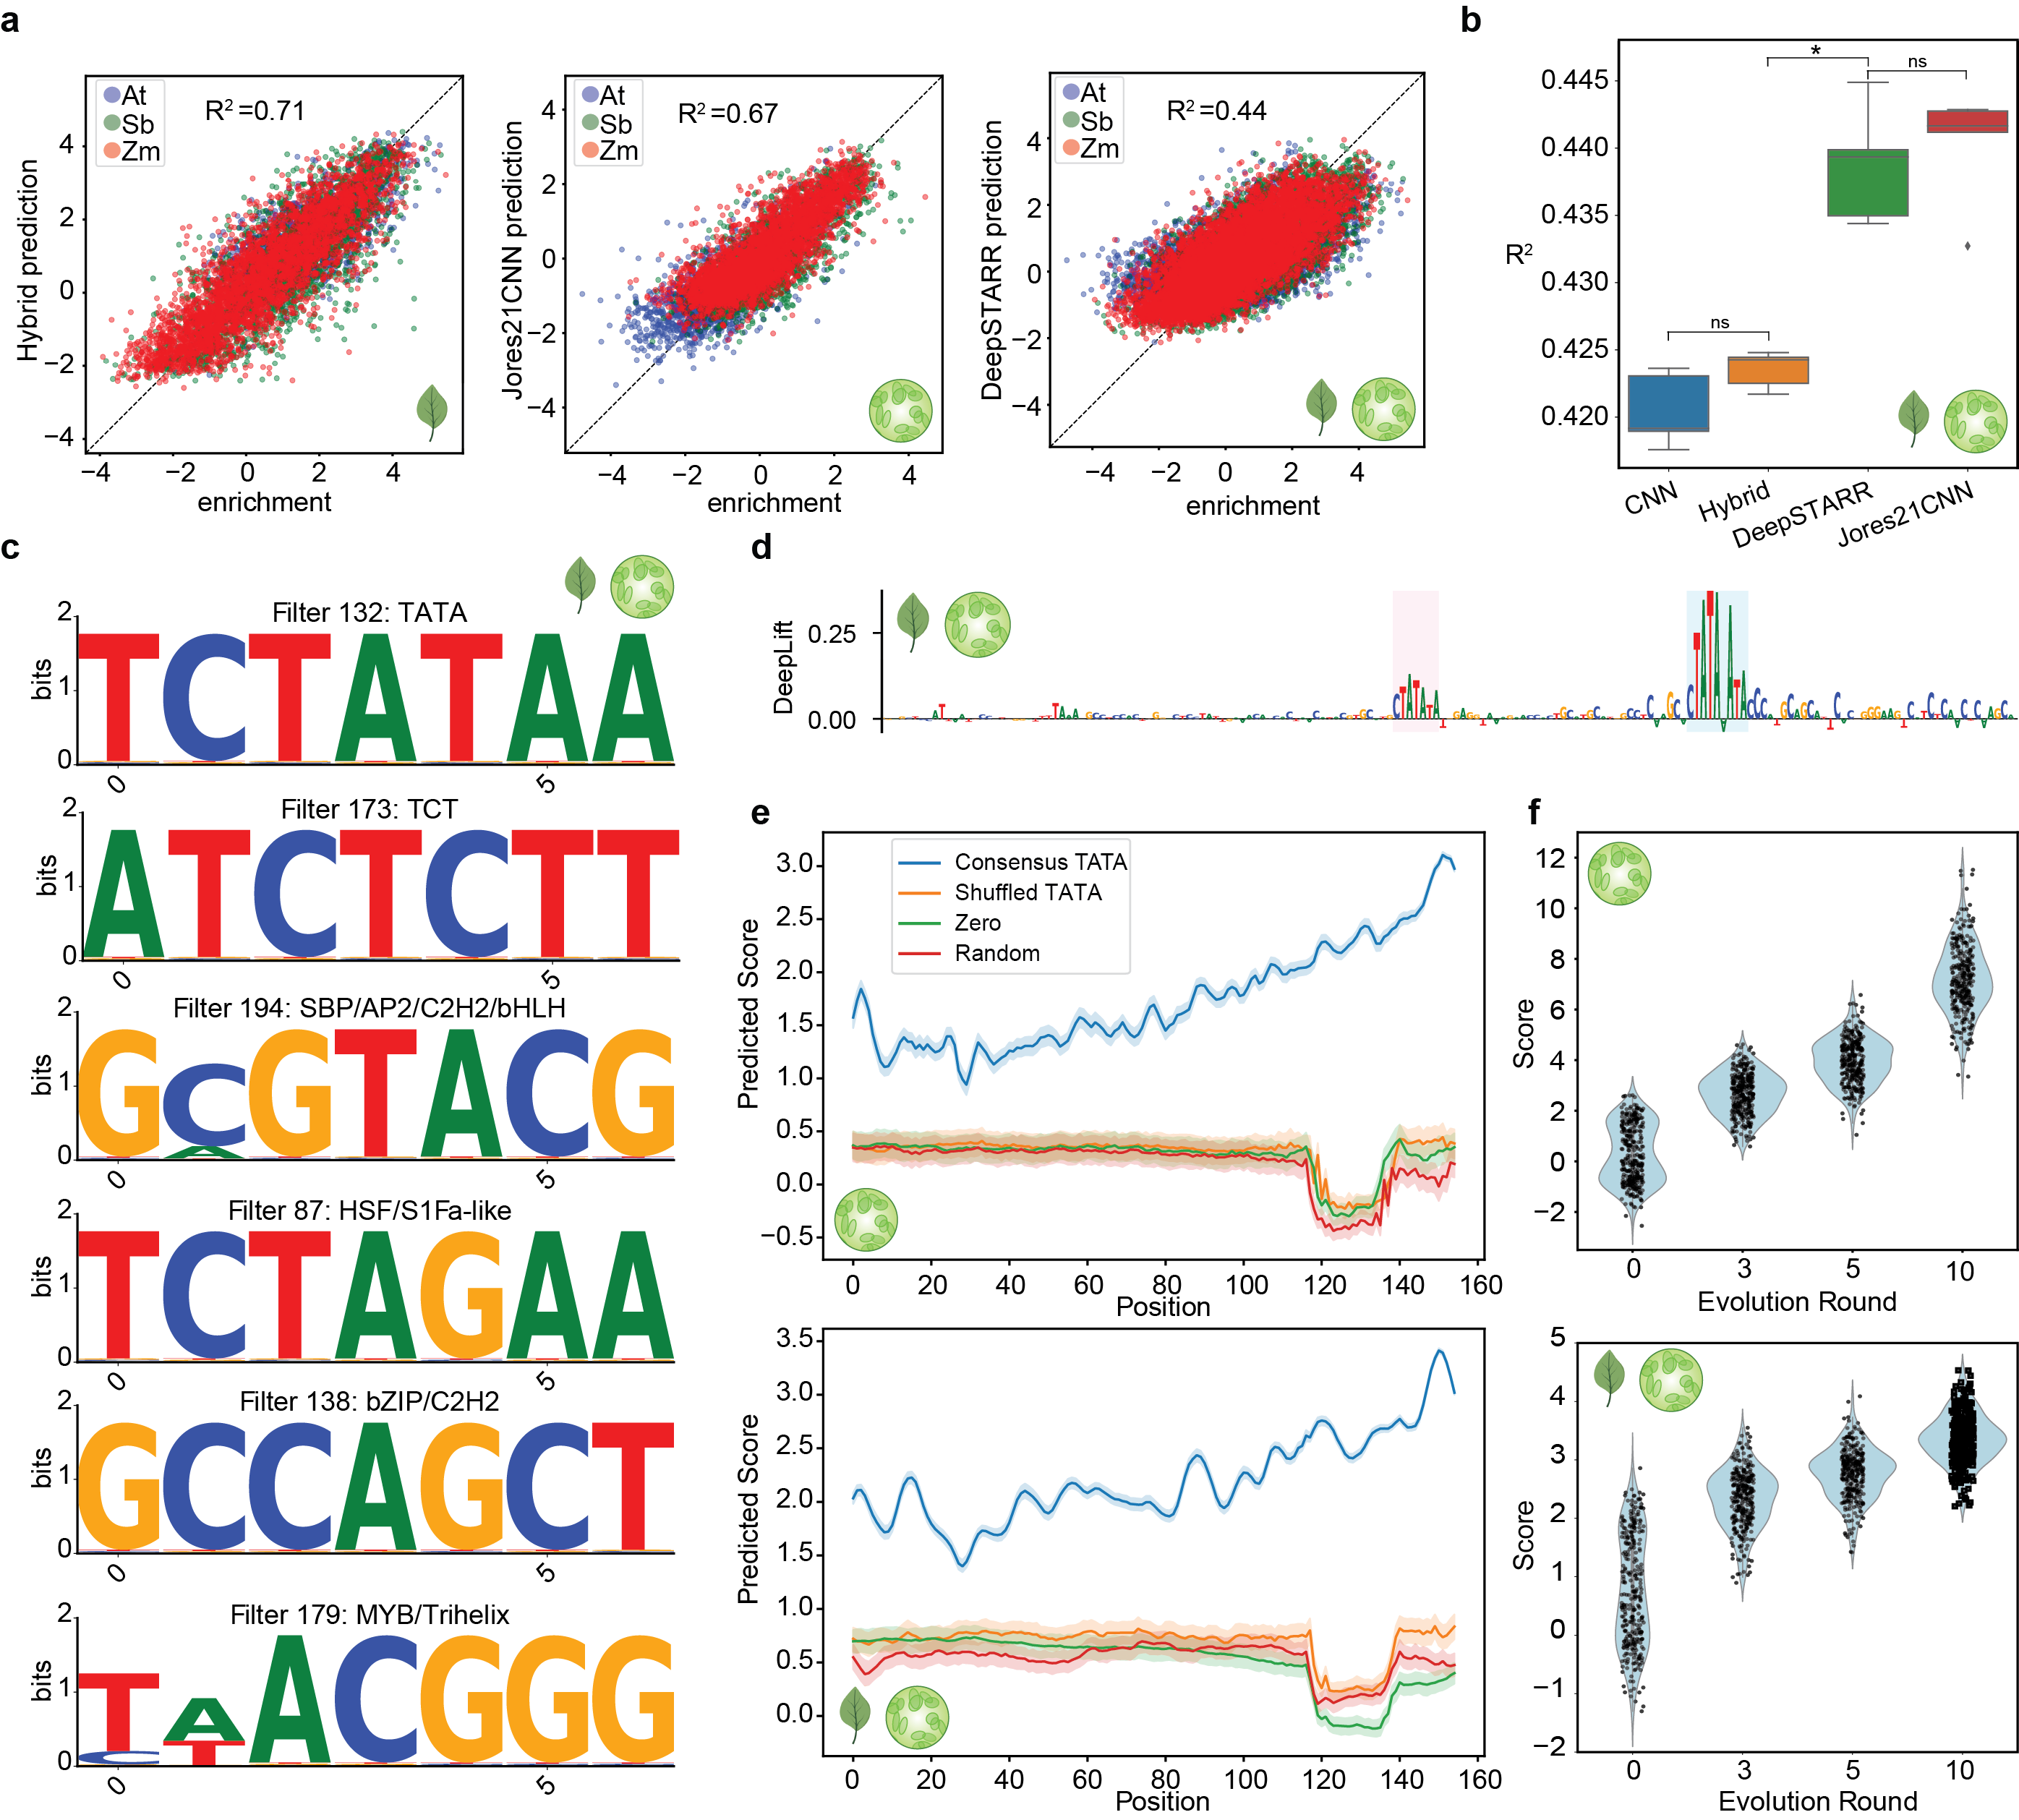
\includegraphics[height=0.5\textheight, keepaspectratio]{1_figures-and-files/suppfigure1.png}
    \caption[STARR-seq supplementary results]{\textbf{STARR-seq plant promoter activity prediction}. \textbf{a}, Performance scatterplots colored by species of origin for the best leaf (left), protoplast (middle) and combined (right) models. \textbf{b}, Predictive performance of all trained combined models. The boxplots show distributions of R2 values on held-out test data for each architecture across n=5 independent experiments (random initializations). The boxes show medians along with low and high quartiles. Whiskers extend to the furthest datapoint within 1.5 times the interquartile range. More extreme points are marked as outliers. A two-sided Mann-Whitney U test was used to determine p-values which were adjusted by the Benjamini-Hochberg method (* = p < 0.05, ns = not significant). Test statistics and adjusted p-values were: CNN-Hybrid (u=4, adjusted p-value=0.11), CNN-DeepSTARR (u=0, adjusted p-value=0.01), CNN-Jores21CNN (u=0, adjusted p-value=0.01), Hybrid-DeepSTARR (u=0, adjusted p-value=0.01), Hybrid-Jores21CNN (u=0, adjusted p-value=0.01), DeepSTARR-Jores21CNN (u=16, adjusted p-value=0.55). \textbf{c}, PWMs for a hand-selected set of learned combined model filters (not initialized with known PWMs). \textbf{d}, Attribution scores calculated using the DeepLIFT method for the sequence with the highest predicted value in the best DeepSTARR combined model. \textbf{e}, Best Jores21CNN protoplast (top) and DeepSTARR combined (bottom) model scores for n=310 sequences with an implanted consensus TATA box motif, shuffled consensus TATA box motif, all zeros motif, and random motif at every possible position. Mean model scores with 95\% confidence intervals are shown. \textbf{f}, Model scores for the same set of n=310 promoters at different rounds of evolution compared against baseline (0) for the best protoplast (top) and combined (bottom) model.}
    \label{fig:1 supplementary_1}
\end{figure}

\begin{figure}[p]
    \centering
    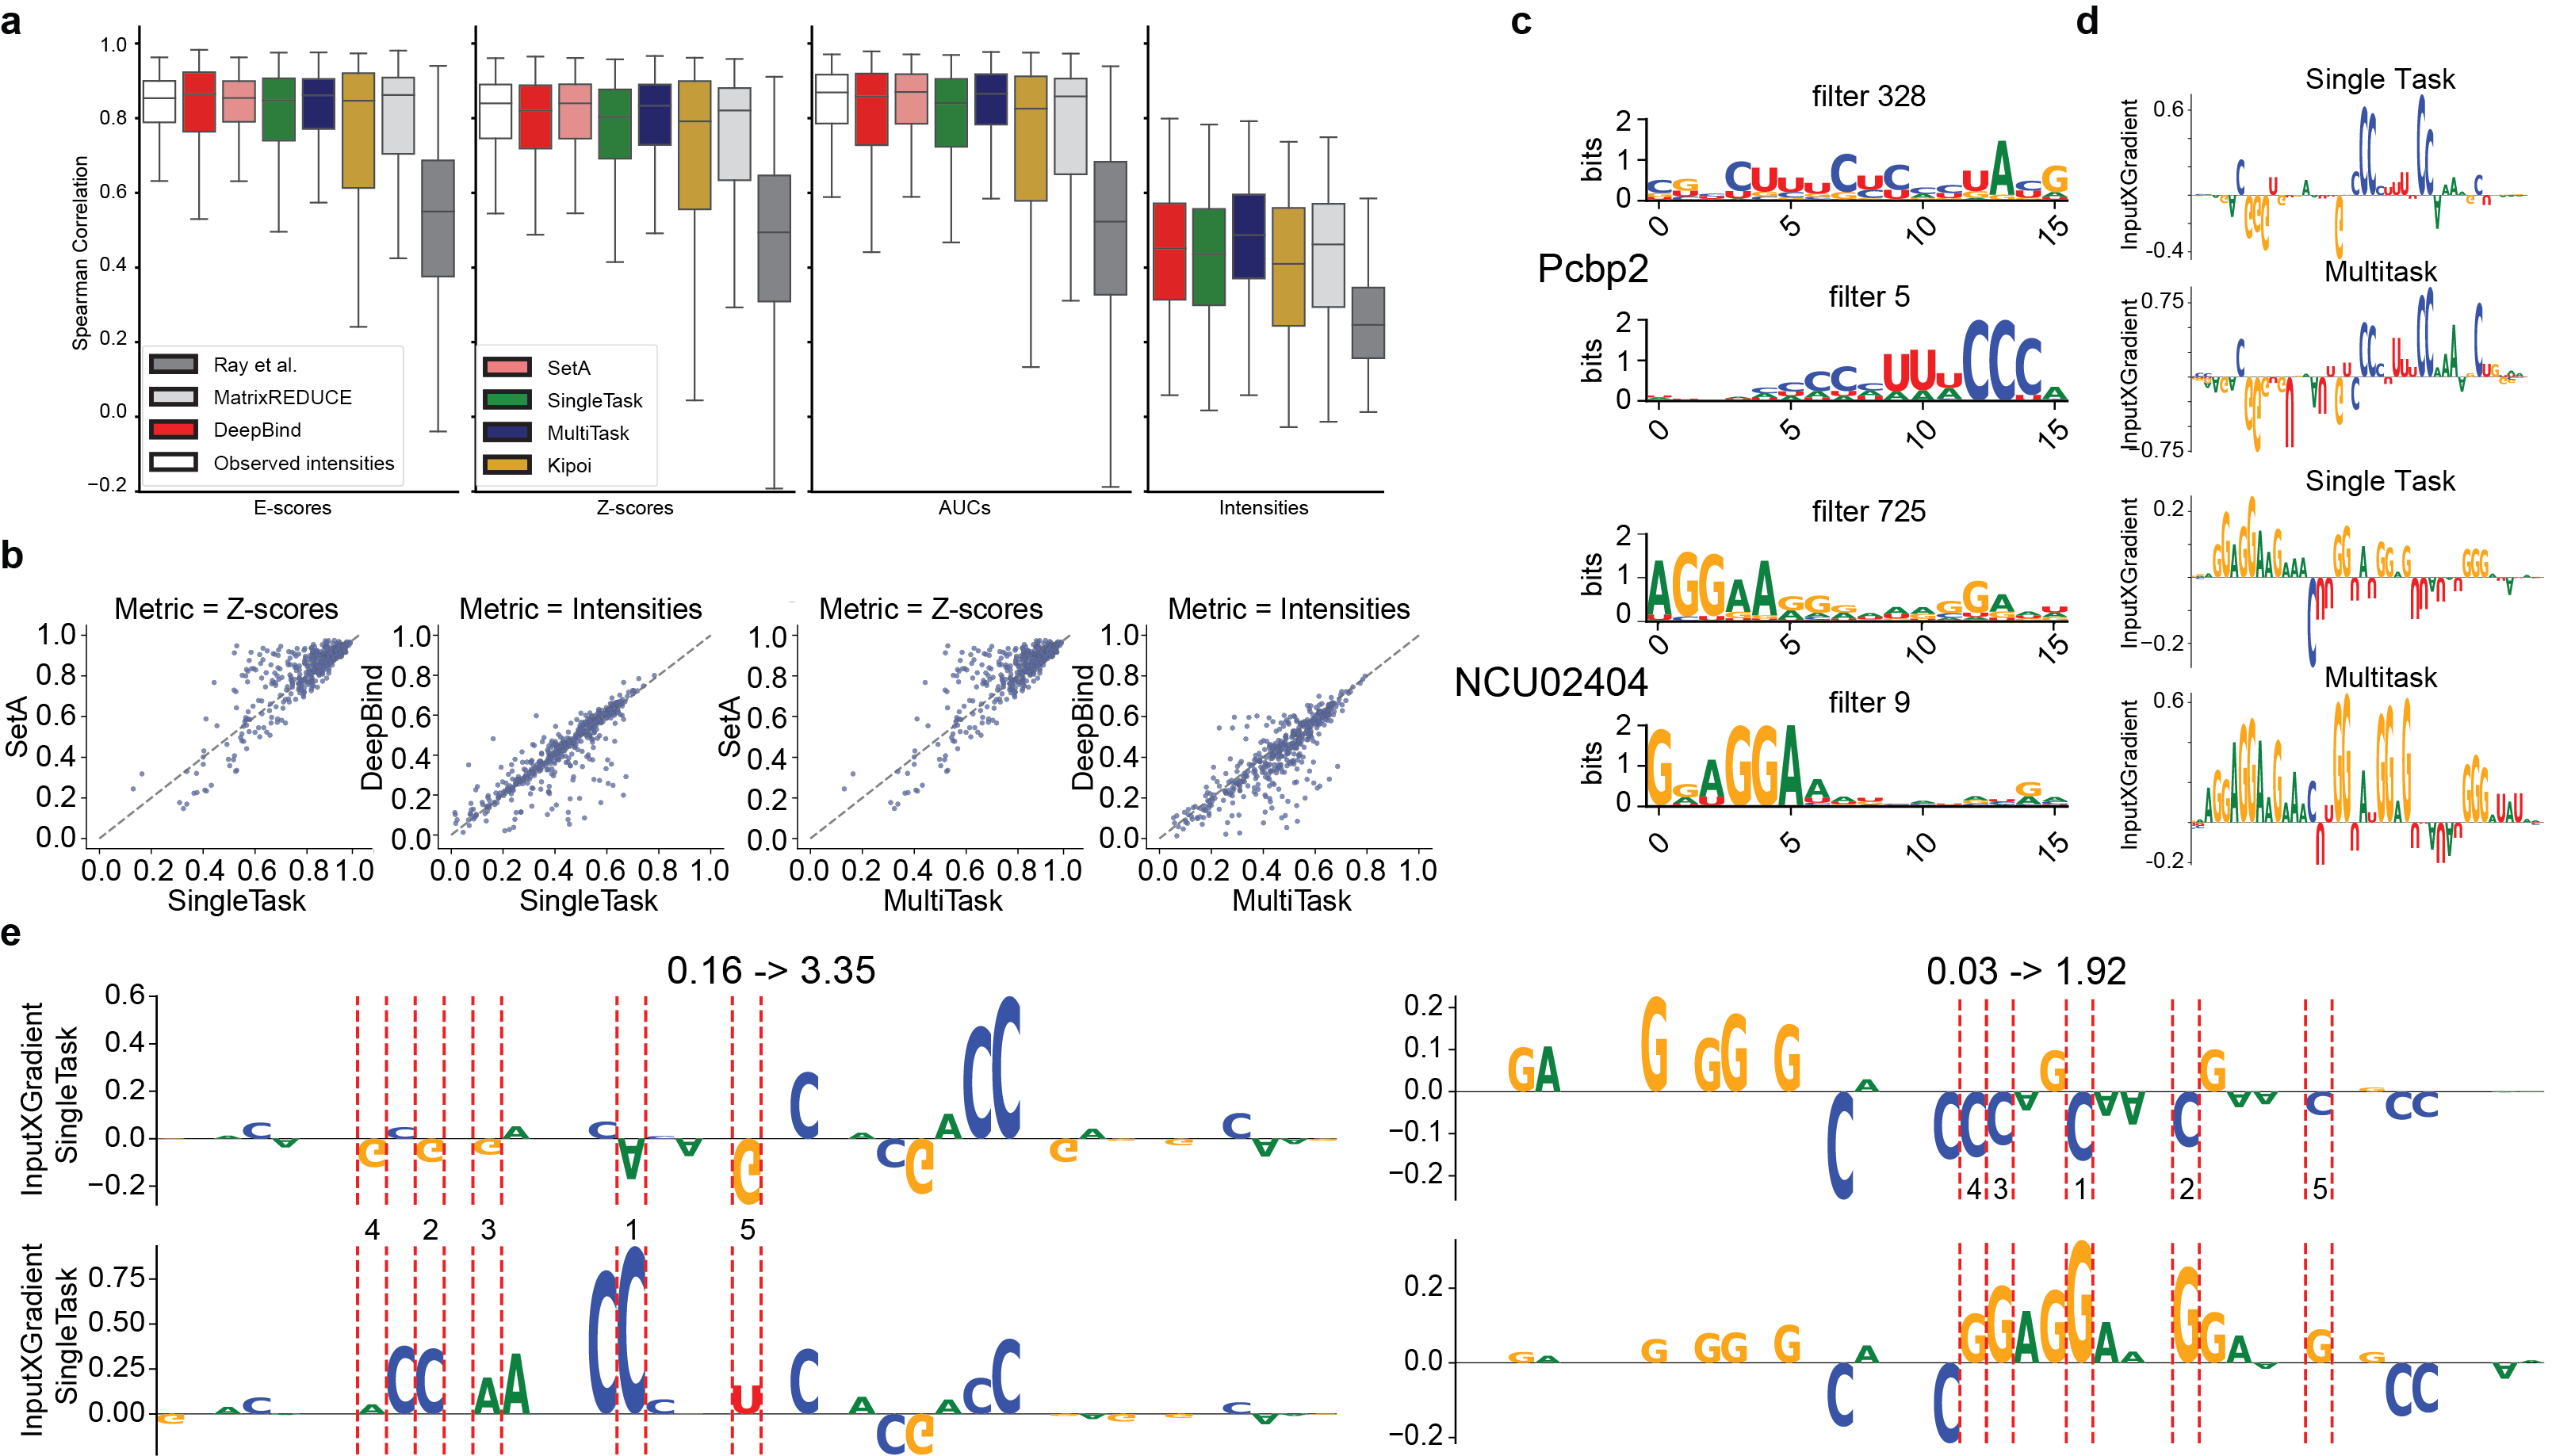
\includegraphics[width=\textwidth]{1_figures-and-files/suppfigure2.png}
    \caption[RBP specificity prediction]{\textbf{RNA binding protein (RBP) specificity prediction}. \textbf{a}, Spearman correlations across four different metrics with each metric calculated from comparisons between observed (Set B) and predicted binding intensities (see Methods for more details on how each metric is calculated). Each boxplot indicates a distribution of Pearson correlations across all n=244 RBPs, except for Kipoi which includes n=89 RBPs. Ray et al, MatrixREDUCE, DeepBind and Observed intensities refer to correlations calculated from predicted intensities reported in Alipanahi et al. Observed intensities and SetA refer to correlations calculated using the intensities from Set A probes as the predicted intensities (see Methods). The boxes show medians along with low and high quartiles. Whiskers extend to the furthest datapoint within 1.5 times the interquartile range. \textbf{b}, Performance comparison scatterplots for the indicated models and metrics. Each dot indicates a comparison of the Pearson correlation between two models on a single RBP. \textbf{c}, Multitask and single task filters with TomTom significant annotations for Pcbp2 (top) and NCU02404 (bottom). \textbf{d}, The feature attributions calculated using the InputXGradient method for single task and multitask models using the sequence with the highest observed intensity in the test set for Pcbp2 (top) and NCU02404 (bottom). \textbf{e}, Two more examples of InputXGradient attribution scores for random (top row) and evolved (bottom row) sequences after evolution with the Pcbp2 (left) and NCU02404 (right) single task models. Red dashed lines indicate mutations made during evolution annotated with the round the mutation occurred in.}
    \label{fig:1 supplementary_2}
\end{figure}

\begin{figure}[p]
    \centering
    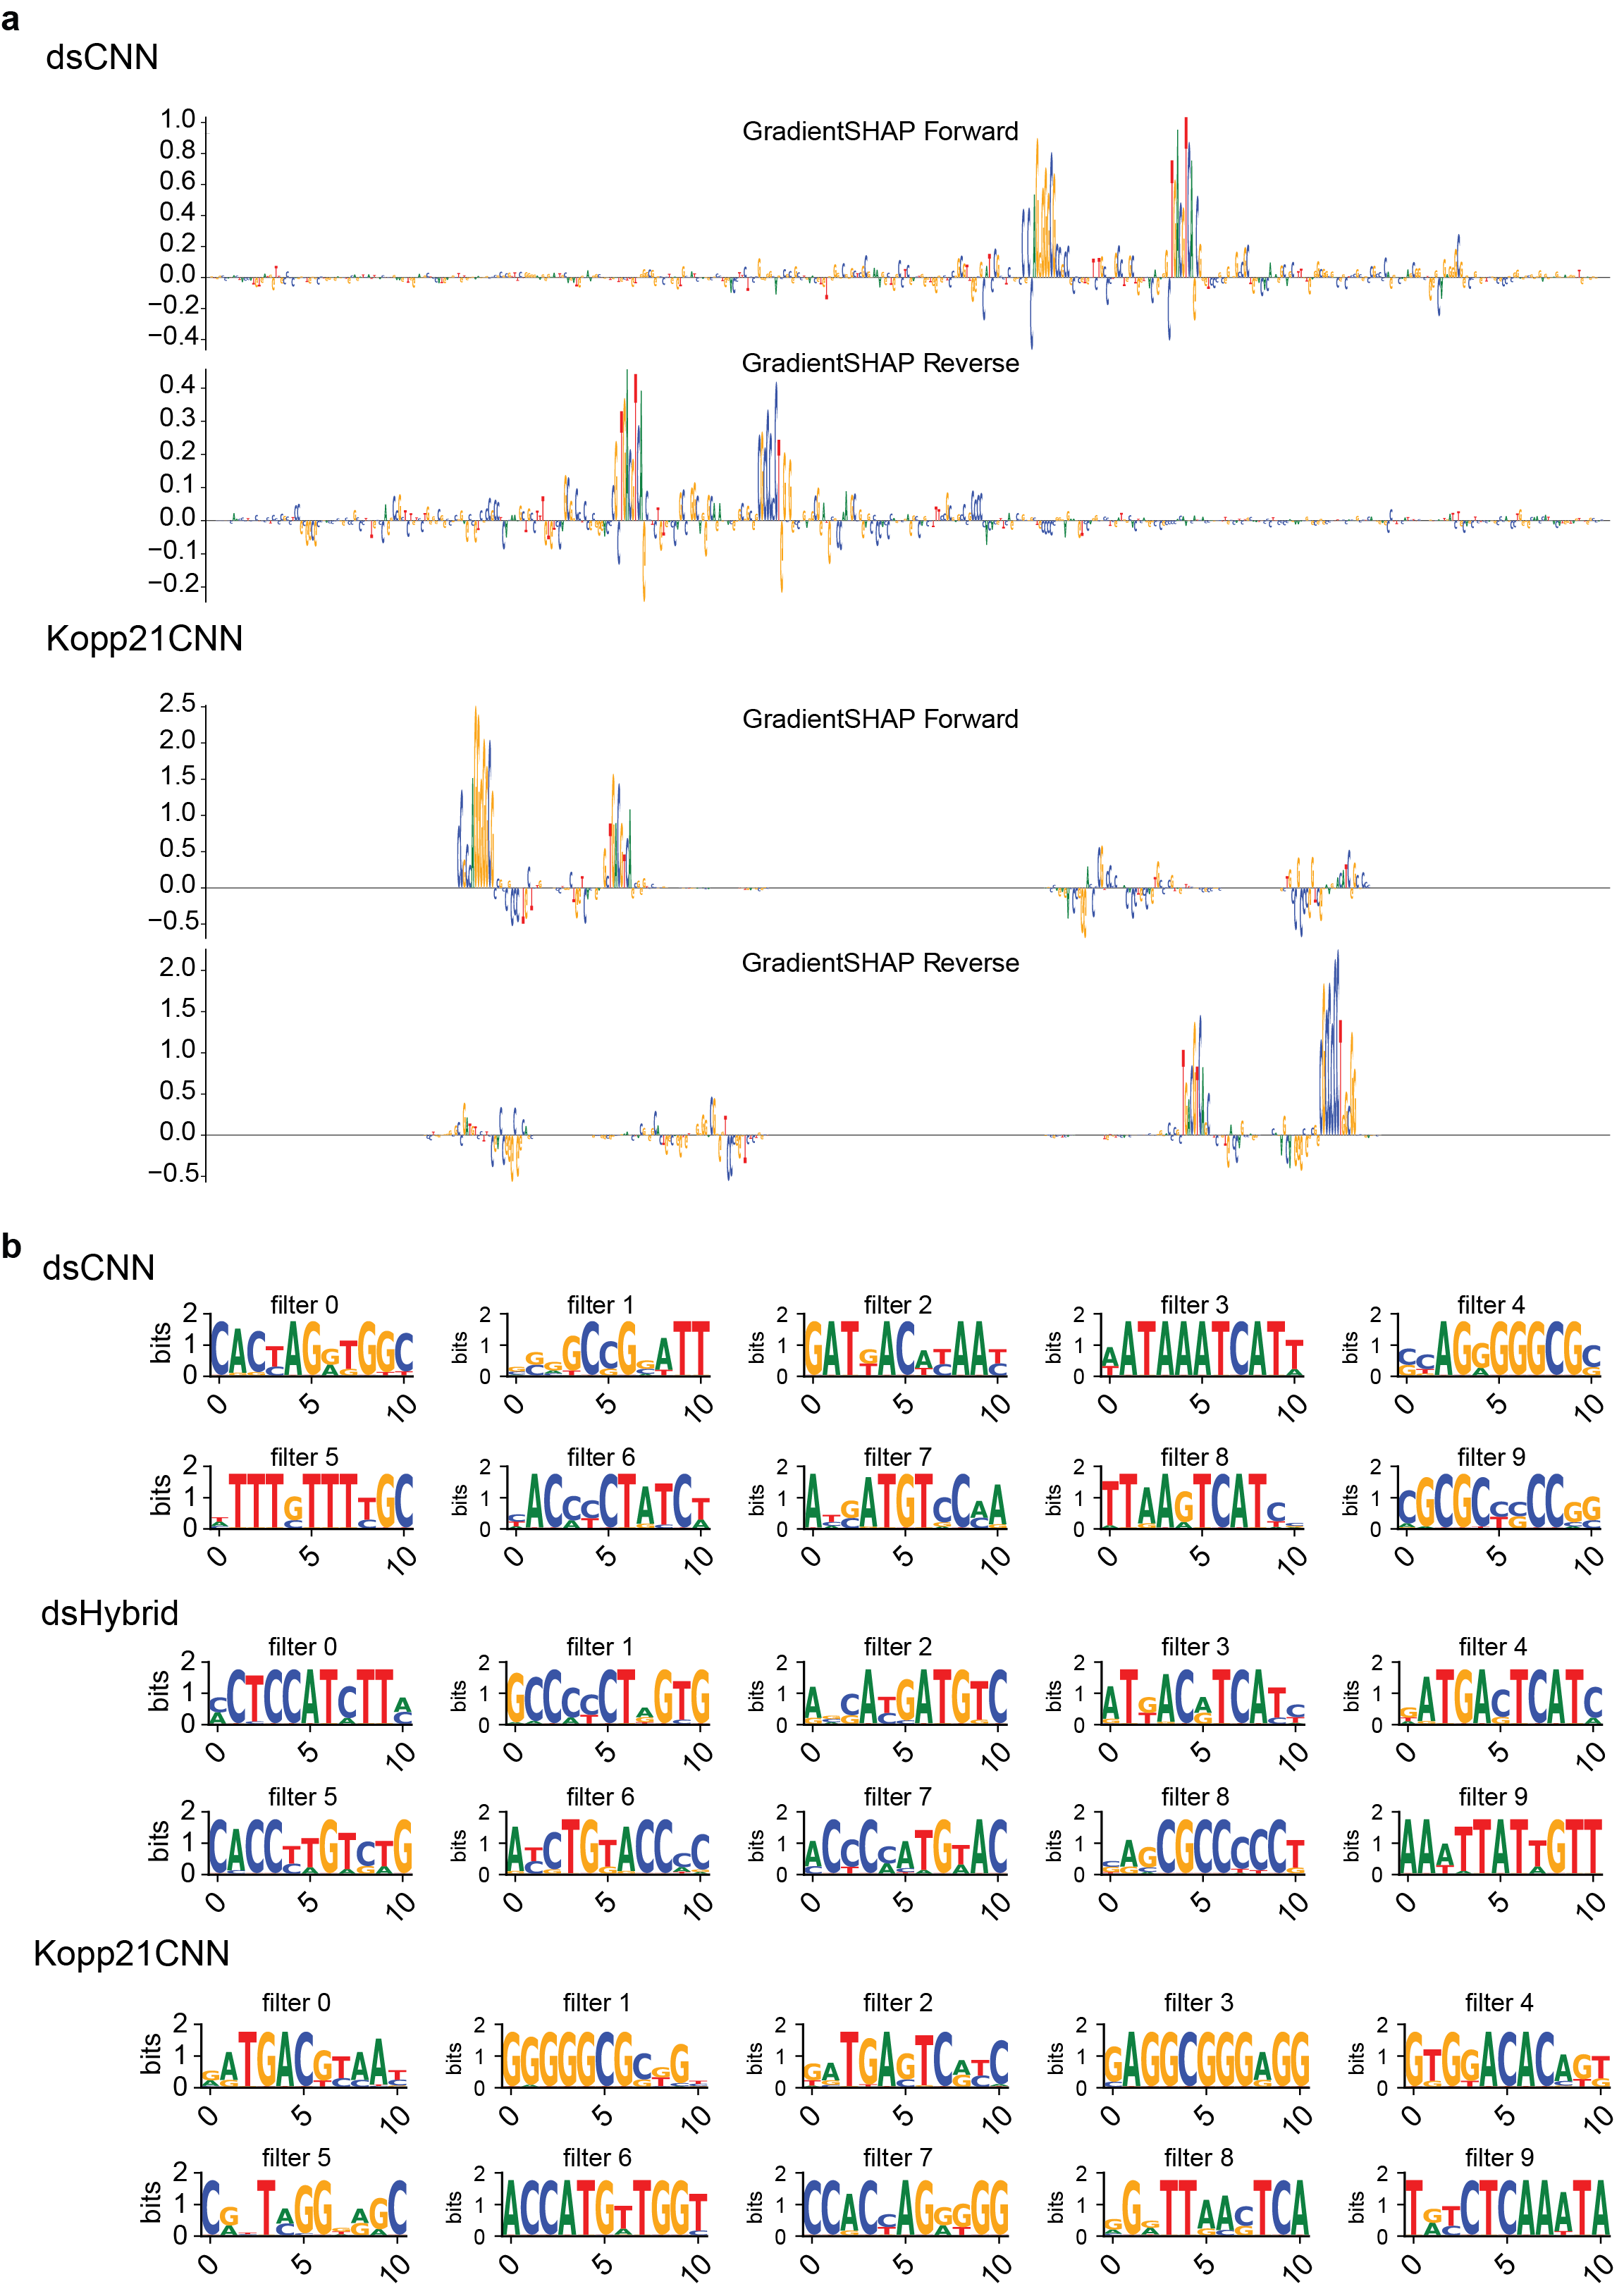
\includegraphics[height=0.65\textheight, keepaspectratio]{1_figures-and-files/suppfigure3.png}
    \caption[JunD classifier interpretation]{\textbf{JunD binding classifier interpretation}. \textbf{a}, Attribution scores calculated using GradientSHAP for the forward and reverse complement of the sequence with the highest predictions in each of the dsCNN and Kopp21CNN models. \textbf{b}, PWM visualizations of the 10 filters for the three convolutional architectures trained for JunD binding classification.}
    \label{fig:1 supplementary_3}
\end{figure}

\begin{figure}[p]
    \centering
    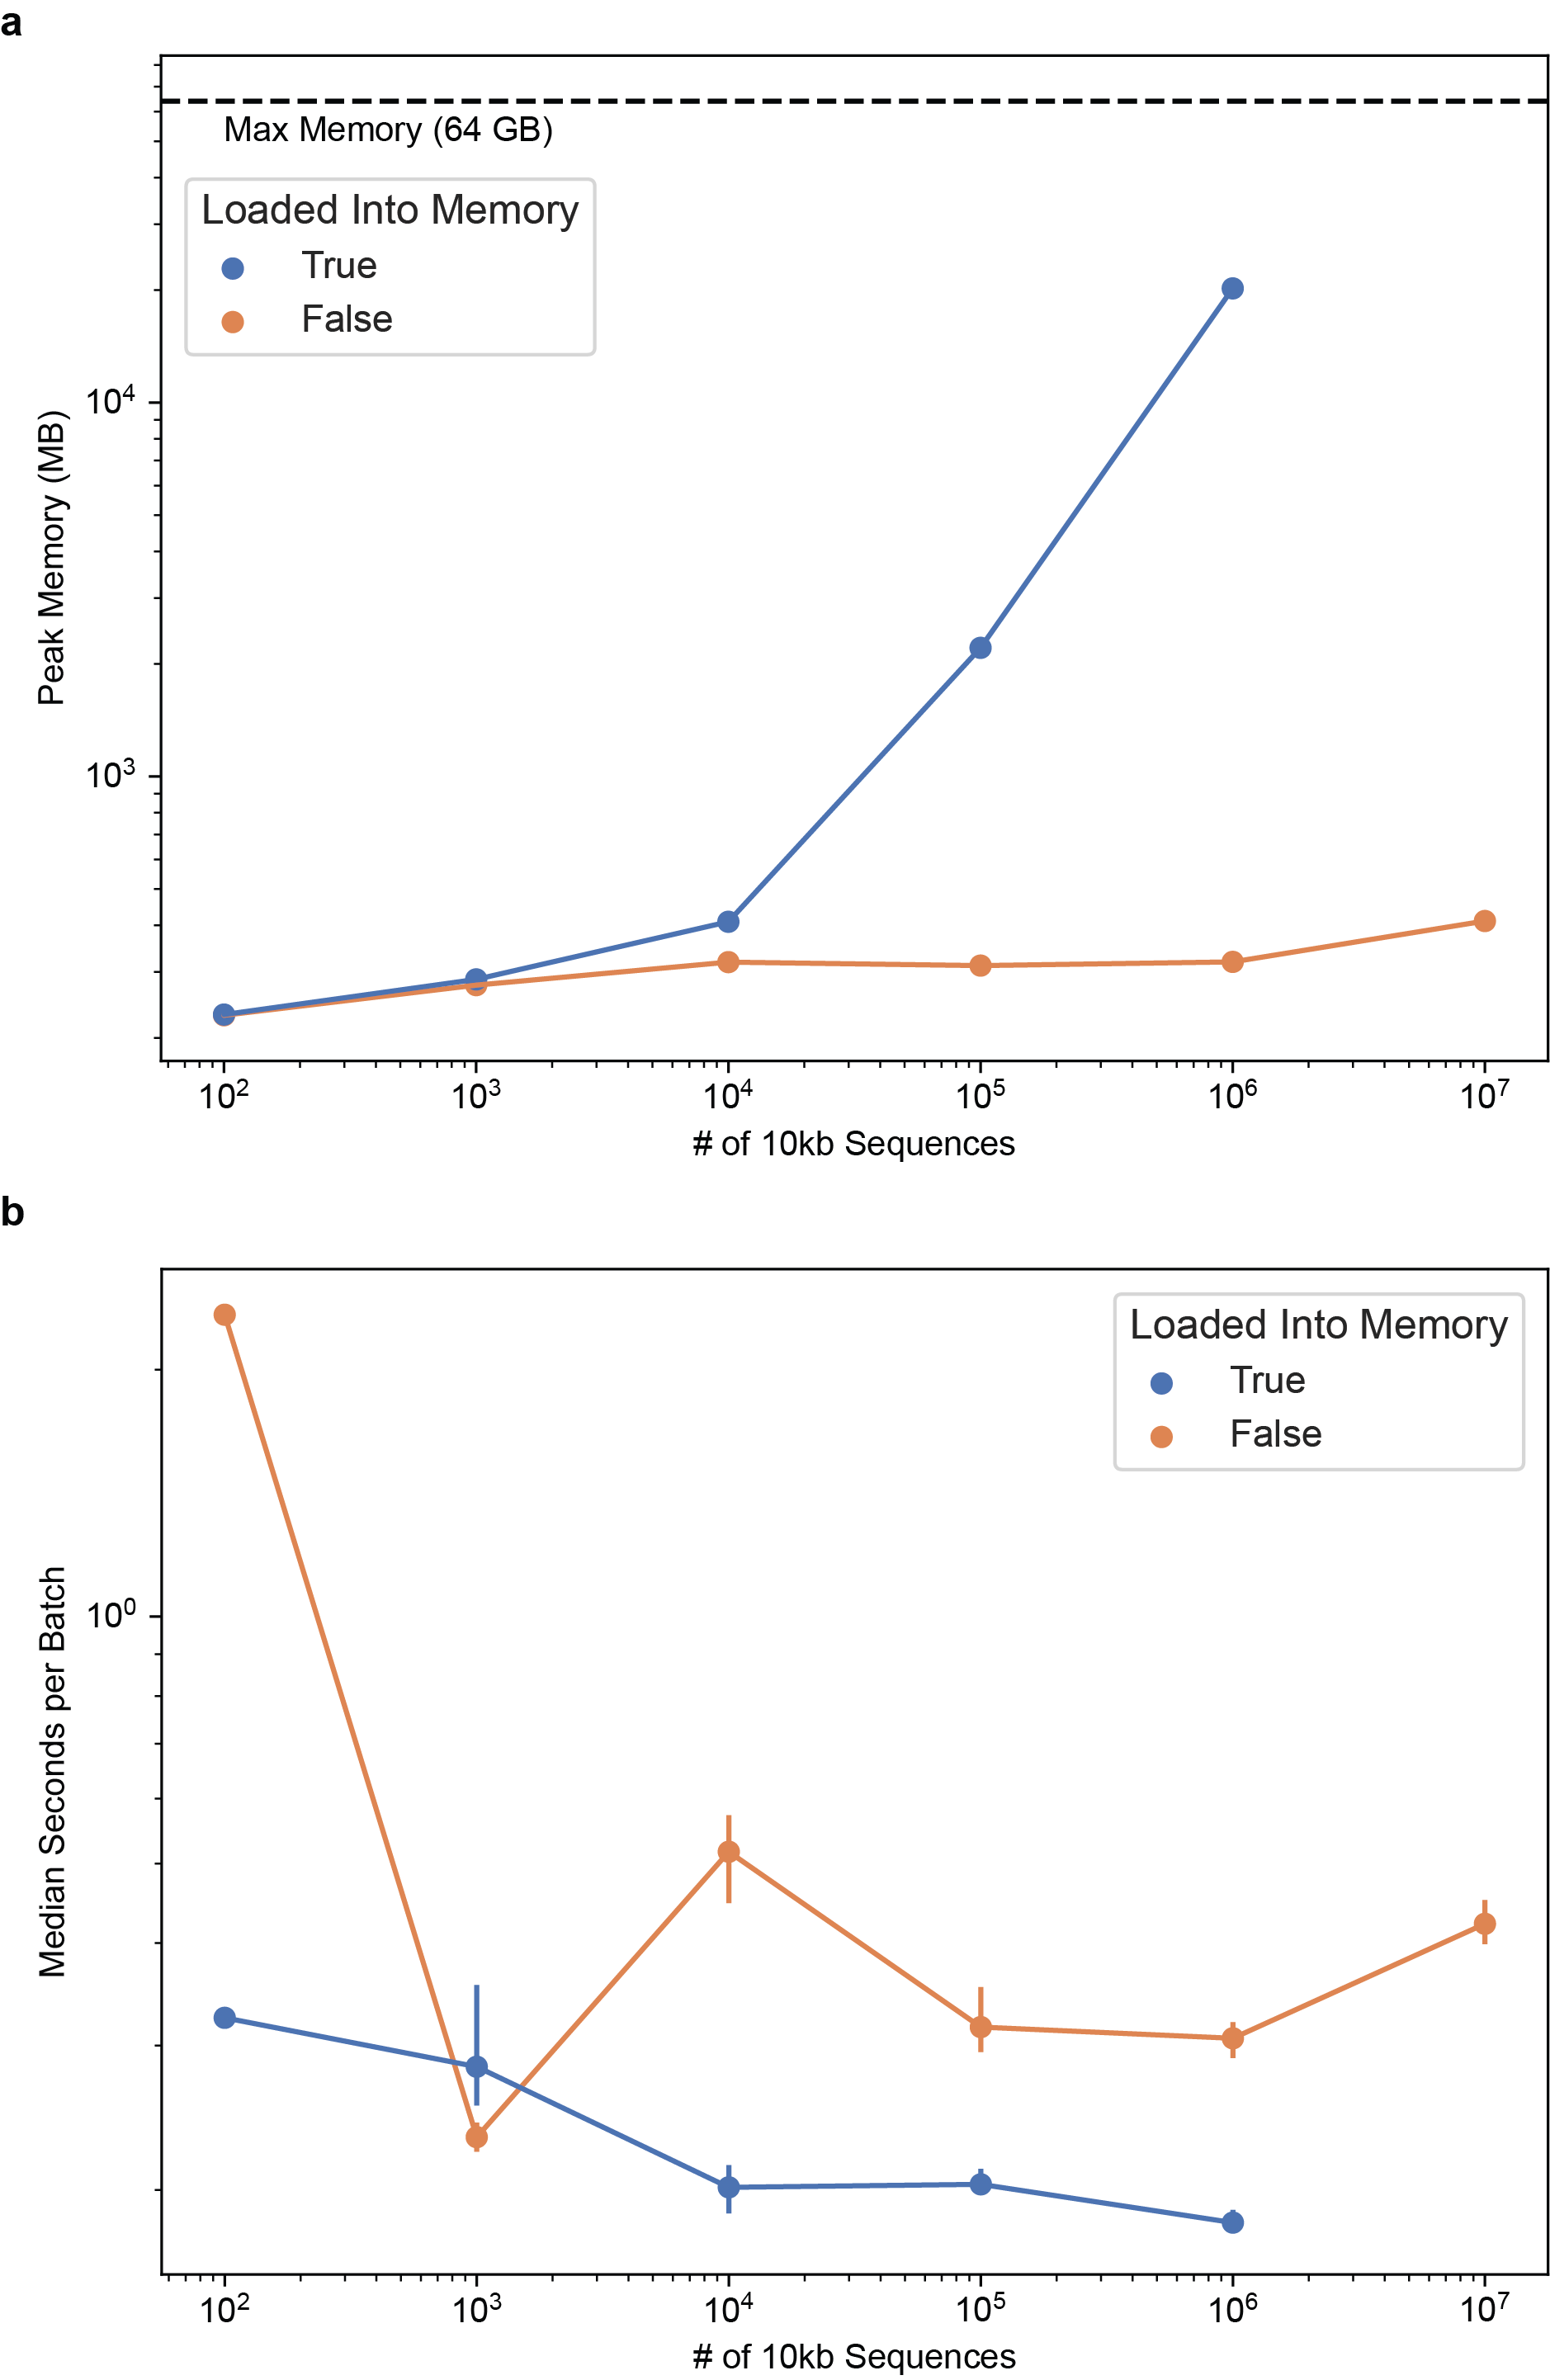
\includegraphics[height=0.65\textheight, keepaspectratio]{1_figures-and-files/suppfigure4.png}
    \caption[Memory and batch time benchmarks]{\textbf{Peak memory usage and batch processing time benchmarks}. Peak memory usage and batch processing time for datasets with increasing numbers of 10,000bp sequences. \textbf{a}, Peak memory usage against number of sequences for datasets loaded into memory versus datasets loaded out-of-core. \textbf{b}, Median time in seconds taken for processing a batch of 100 sequences using the same datasets as in \textbf{a}. Error bars indicate interquartile ranges across up to 100 random batches. Both axes in \textbf{a} and \textbf{b} are on the log10 scale. All analyses were performed using a chunk size of 4096 along the sequence dimension on a machine with 2 CPU cores and 64GB of RAM.}
    \label{fig:1 supplementary_4}
\end{figure}

\begin{figure}[p]
    \centering
    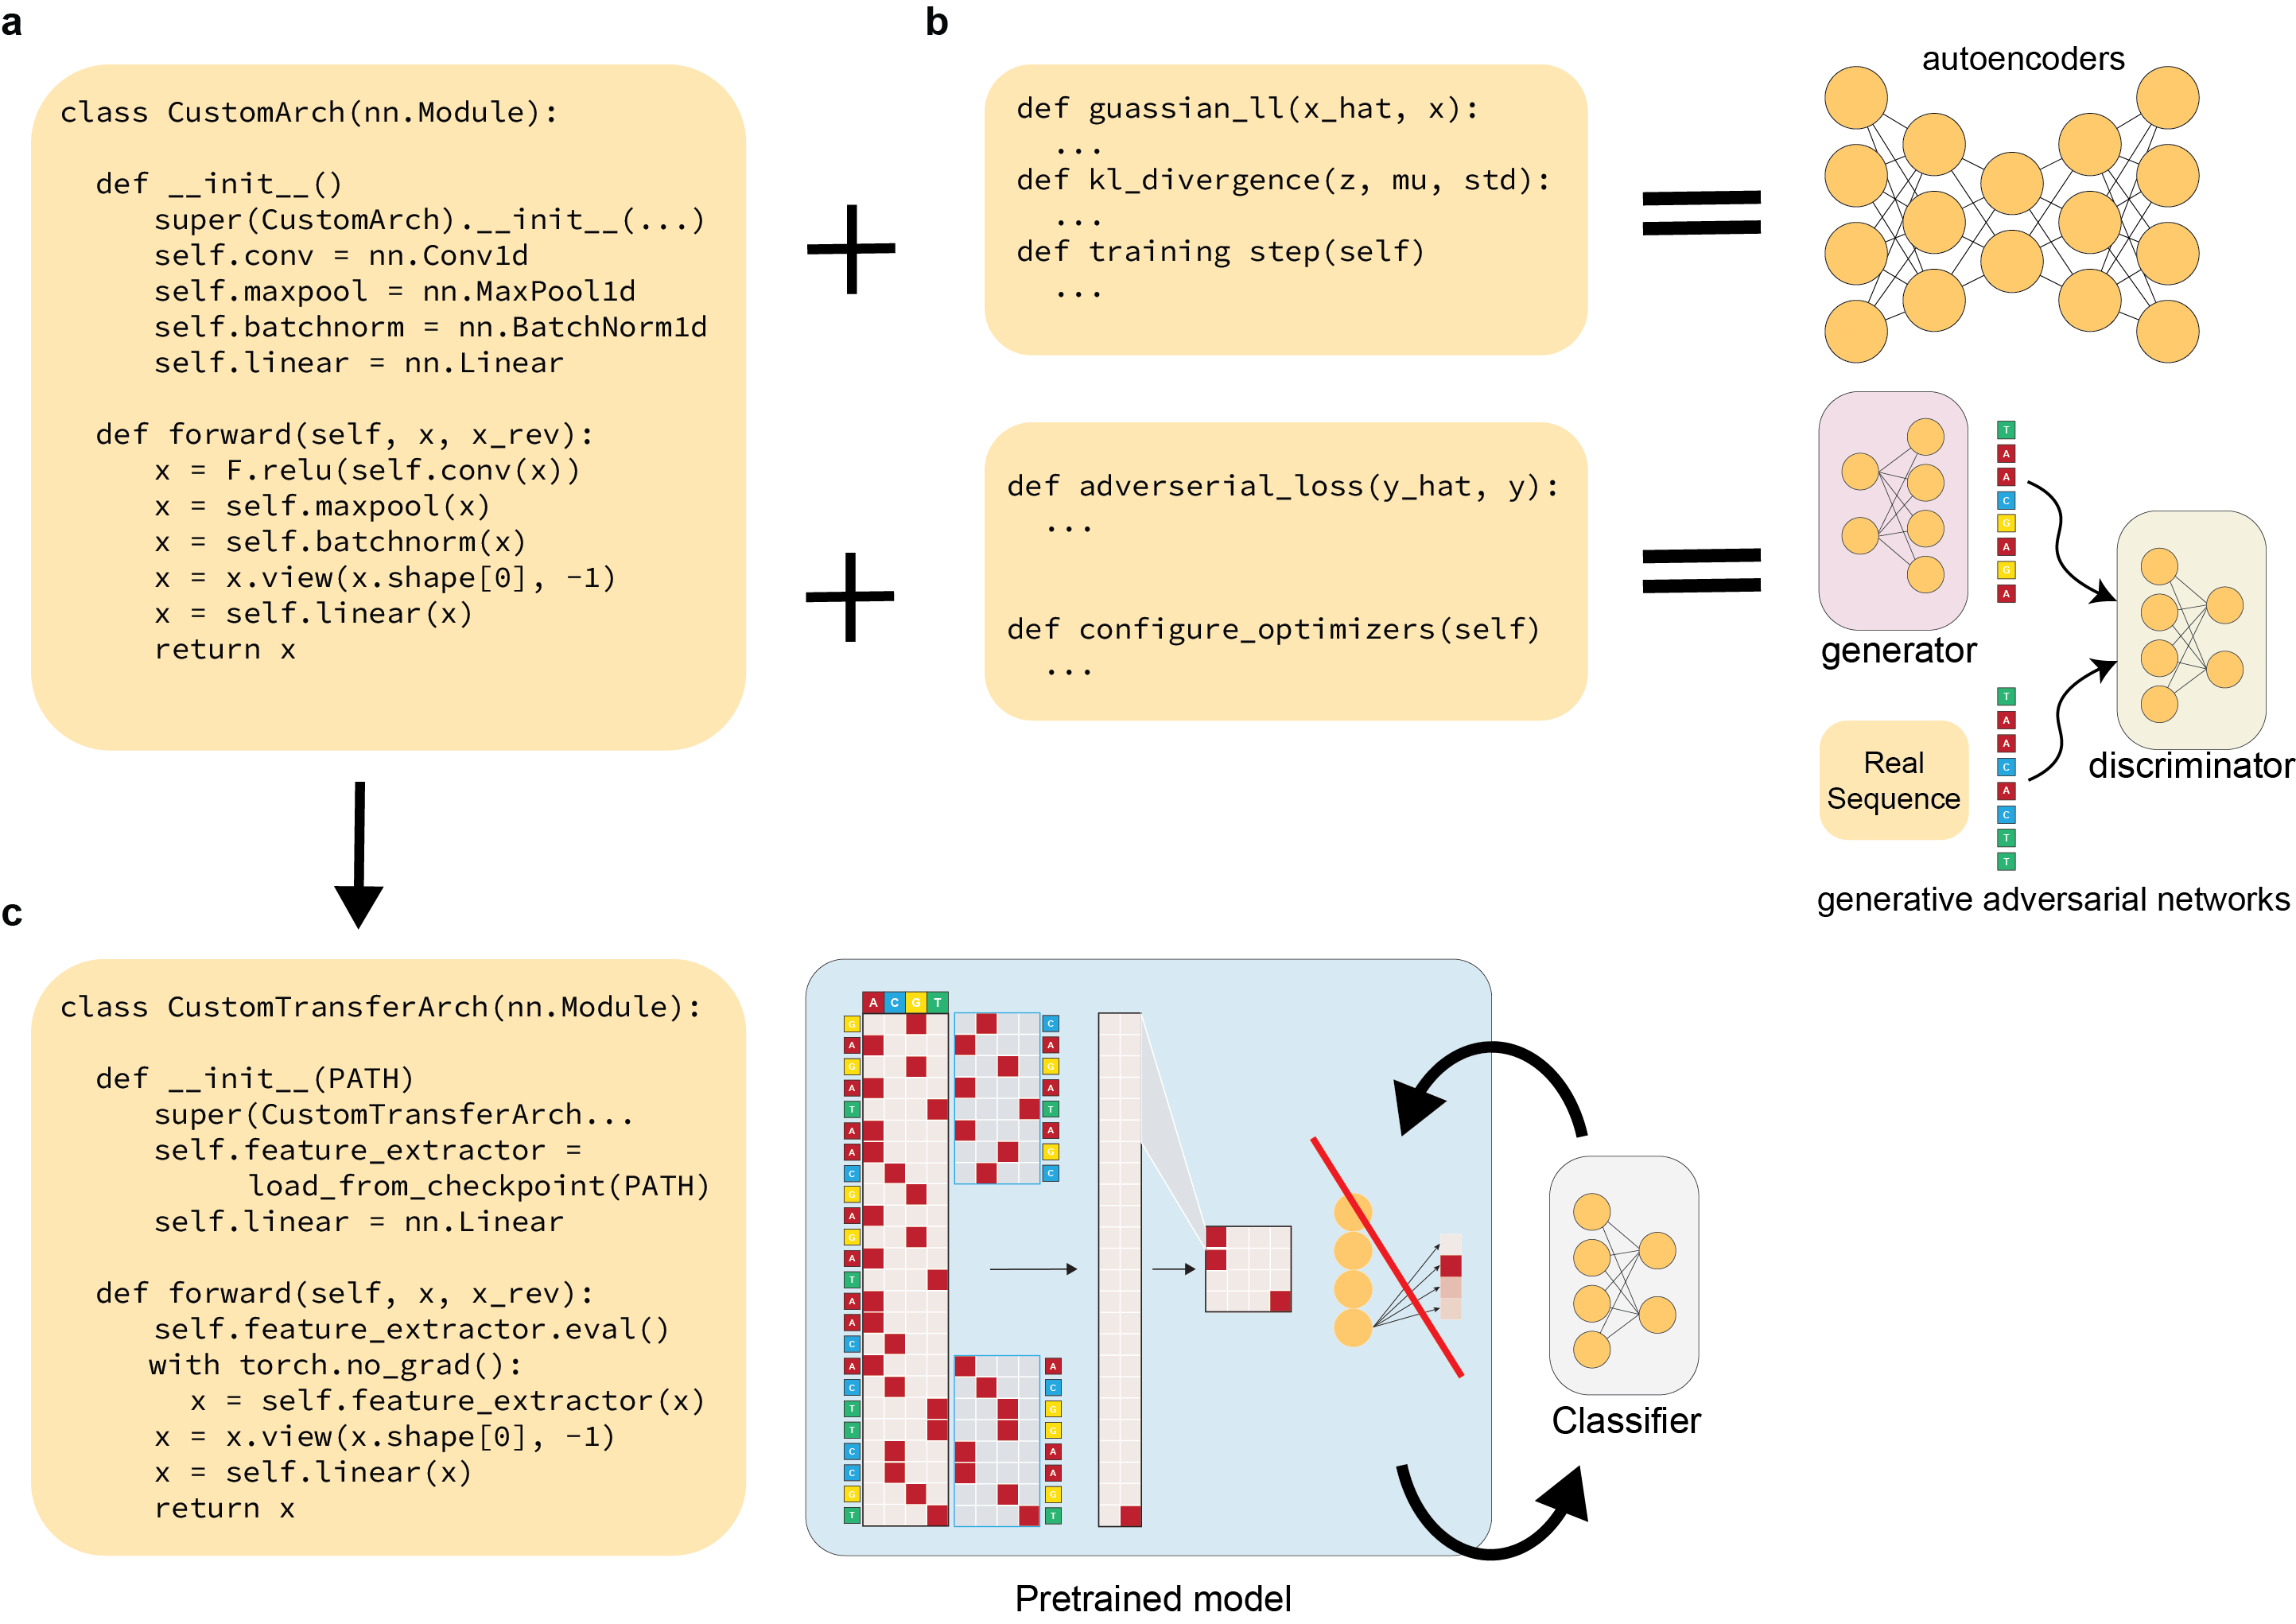
\includegraphics[width=\textwidth]{1_figures-and-files/suppfigure5.png}
    \caption[Custom model development in EUGENe]{\textbf{Implementing custom architectures and training tasks in EUGENe}. \textbf{a}, Creating custom architectures that are compatible with EUGENe’s training protocol involves first inheriting from the \texttt{torch.nn.Module} class, then defining the model’s layer composition (\texttt{init}) and the forward propagation (\texttt{forward}) method. \textbf{b}, Architectures can also be wrapped in \texttt{LightningModules} to allow for training protocols other than EUGENe’s current built-ins. For instance, a variational autoencoder, or VAE, requires creating two functions for calculating different parts of the loss and implementing how the functions are integrated into the training function (in its most basic form). We have omitted the changes needed to define an encoder and decoder structure and how that is handled in \texttt{forward}. A generative adversarial network (GAN), as another example, requires implementing a multipart loss function and configuring multiple optimizers to handle the training of the generator and discriminator. \textbf{c}, Transfer learning from pretrained models is also possible in EUGENe, and can be accomplished with simple changes to an architecture’s initialization and \texttt{forward} functions. Namely, a pretrained PyTorch model needs to be loaded in the (\texttt{forward}) method and then utilized in the \texttt{forward} method.}
    \label{fig:1 supplementary_5}
\end{figure}

\chapter{Supplemental Material for Chapter \ref{chap:chapter 2}}

%%%%%%%%%%%%%%%%%%%%%%%%%%%%%%%%%%%%%%%%%%%%%%%%%%%%%%%%%%%%%%%%%%%%%%%%%%%%%%%%
\section{Supplementary Figures}
%%%%%%%%%%%%%%%%%%%%%%%%%%%%%%%%%%%%%%%%%%%%%%%%%%%%%%%%%%%%%%%%%%%%%%%%%%%%%%%%

\begin{figure}[p]
    \centering
    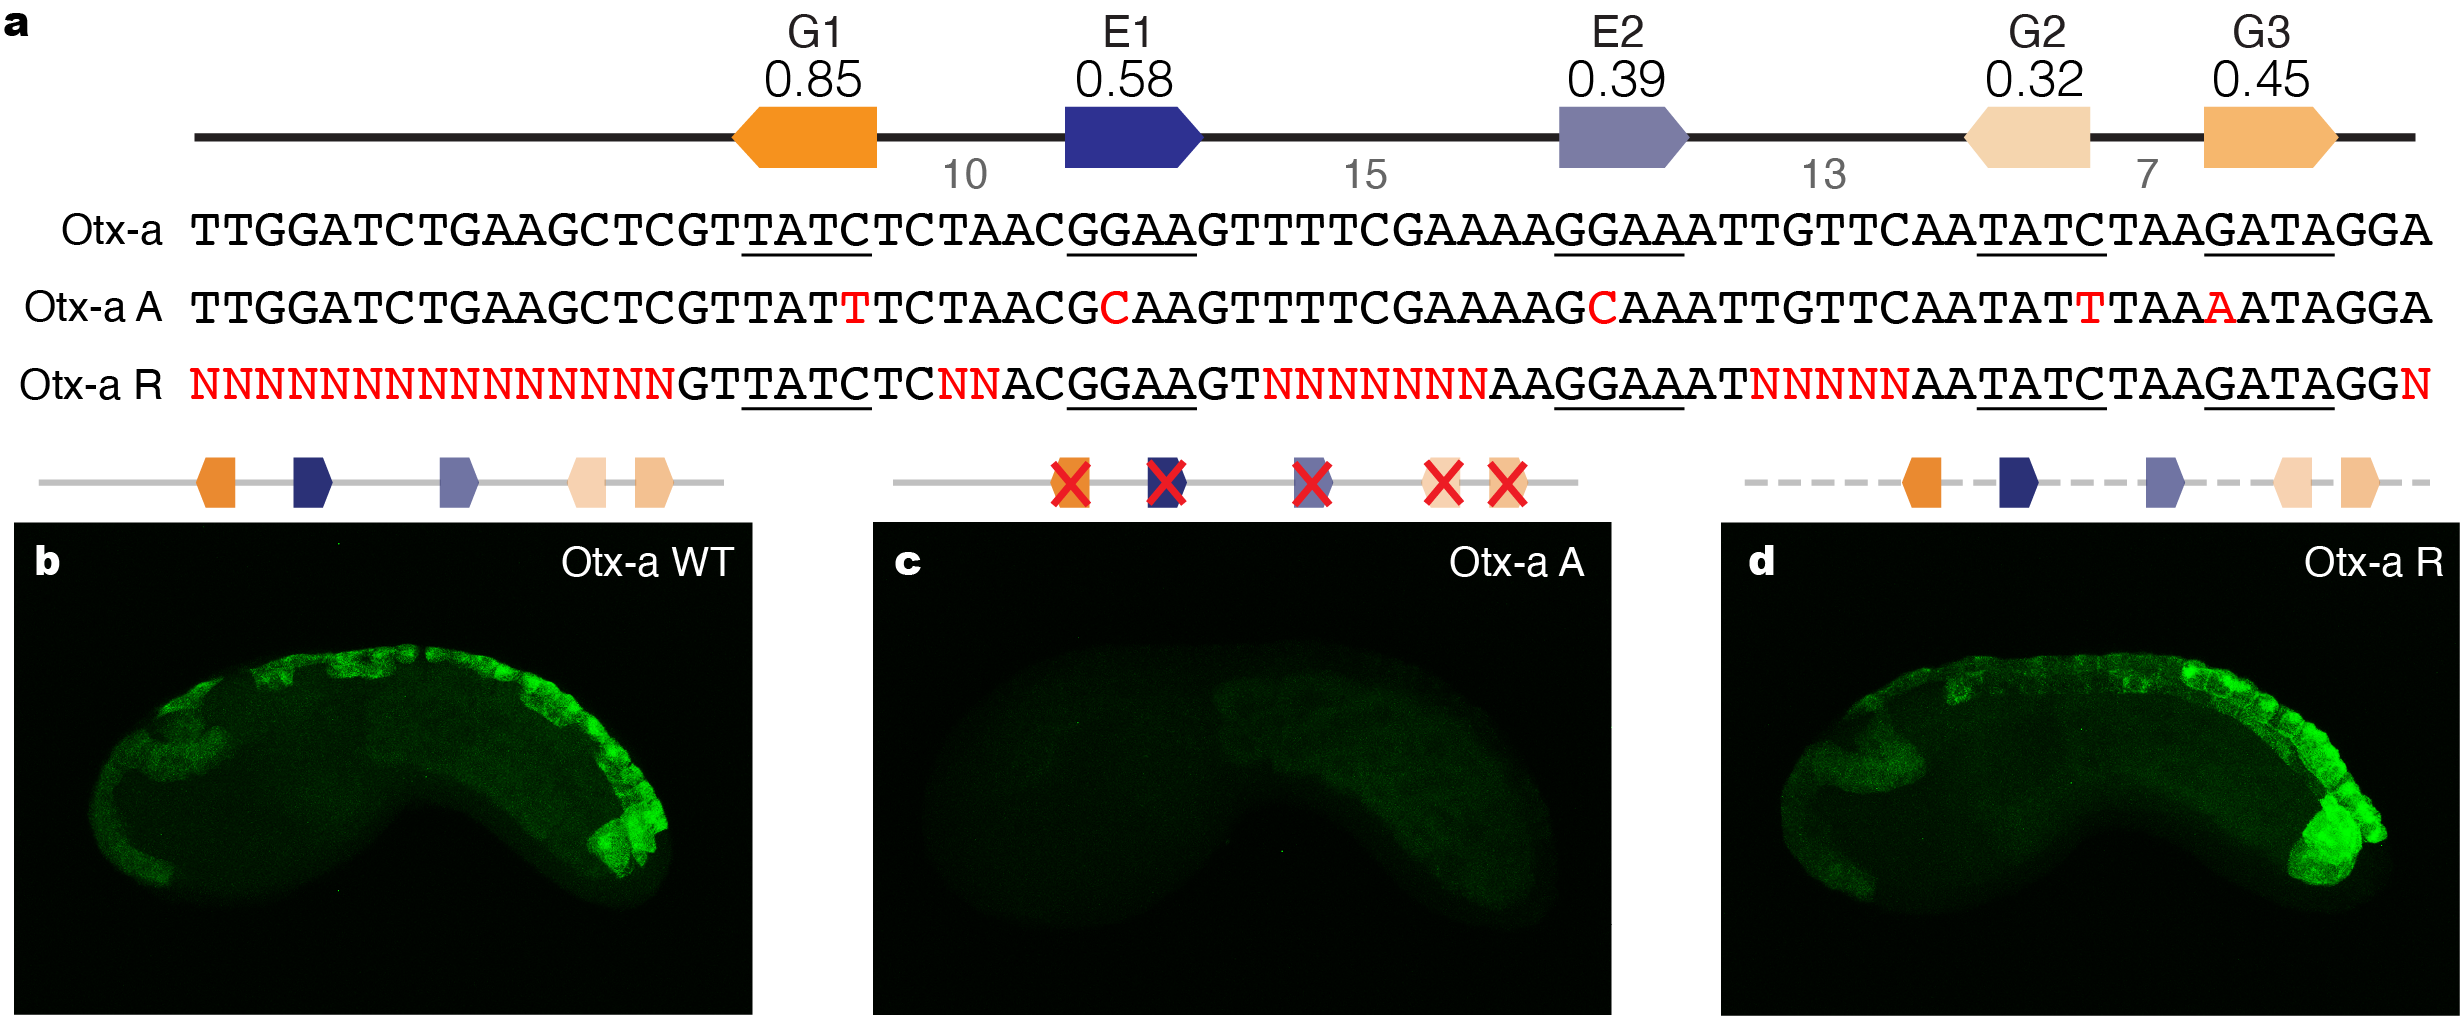
\includegraphics[width=0.85\textwidth]{2_figures-and-files/SuppFig1.png}
    \caption[Defining the necessary and sufficient TFBS for Otx-a enhancer activity.]{\textbf{Defining the necessary and sufficient TFBS for Otx-a enhancer activity.} \textbf{a)} Otx-a contains three GATA and two ETS sites. The GATA and ETS core sequences that hydrogen bond to the TF are underlined, GATA and GGAW respectively. The relative affinity is labelled above each site and is defined by the nucleotides flanking the cores. Spacing between the sites is shown in gray numbers. Otx-a Ablated (Otx-a A) contains single point mutations within the core of each binding site that ablate binding of the TF. The Otx-a Randomized (Otx-a R) library contains 5 million unique sequences where the GATA and ETS sites are fixed, but the linker sequences are randomized (denoted with Ns which represent equal chance of A, T, G or C). \textbf{e)} Otx-a WT enhancer activates expression in the a6.5 and b6.5 lineages. \textbf{f)} Otx-a A does not activate expression. \textbf{g)} Otx-a R activates neural expression that is indistinguishable from Otx-a WT despite the randomization of linker sequences.}
    \label{fig:2 supplementary_1}
\end{figure}

\begin{figure}[p]
    \centering
    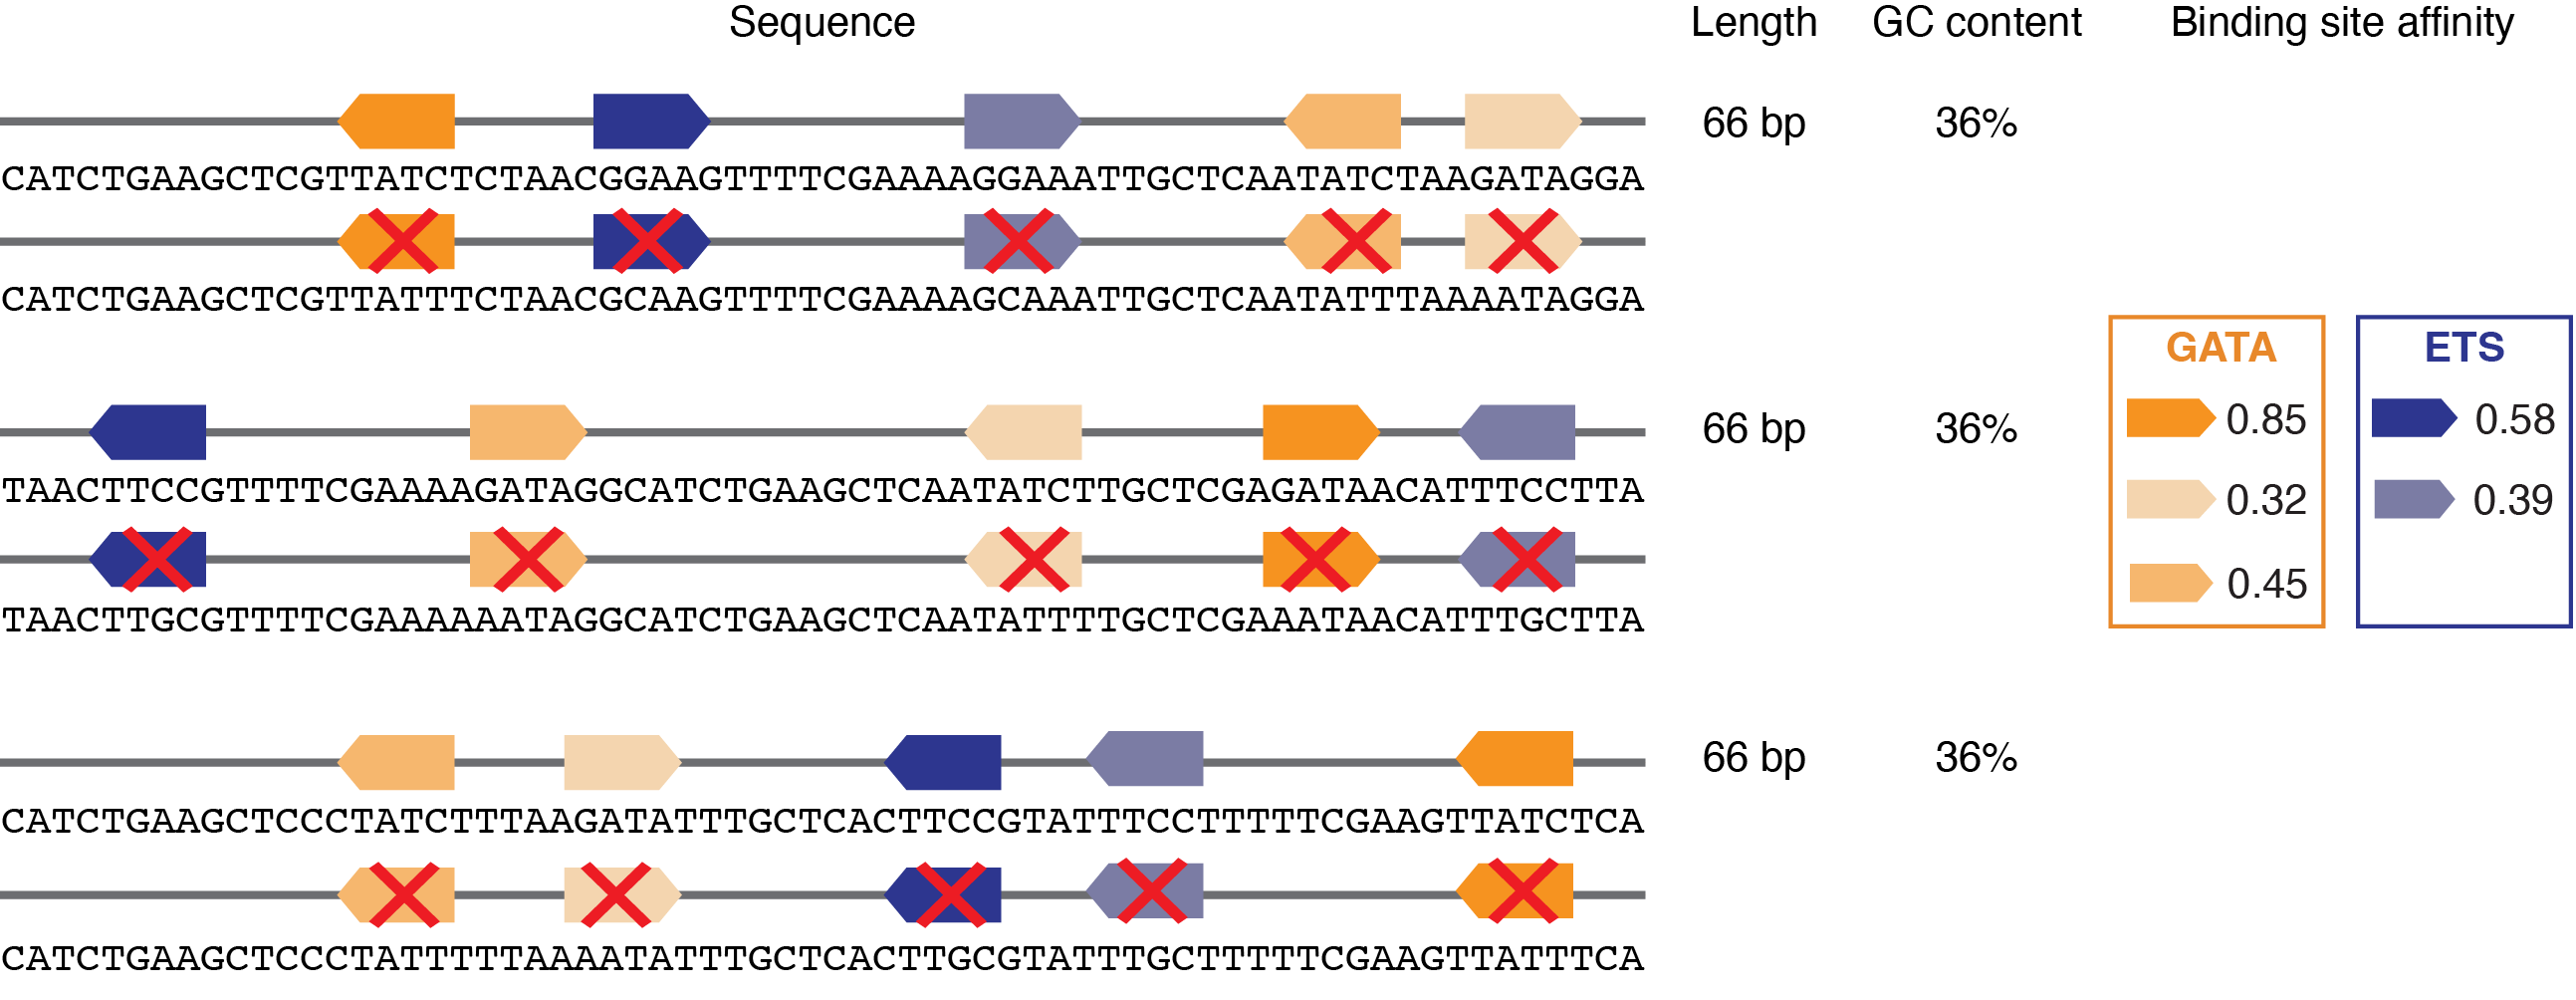
\includegraphics[width=0.75\textwidth]{2_figures-and-files/SuppFig2.png}
    \caption[Examples of Otx-a scrambled library variants and their ablated counterparts.]{\textbf{Examples of Otx-a scrambled library variants and their ablated counterparts.} Each element has the same sequence content, GC content, and binding sites. The only difference between the members is the order, orientation, spacing and placement of the different affinity binding sites.}
    \label{fig:2 supplementary_2}
\end{figure}

\begin{figure}[p]
    \centering
    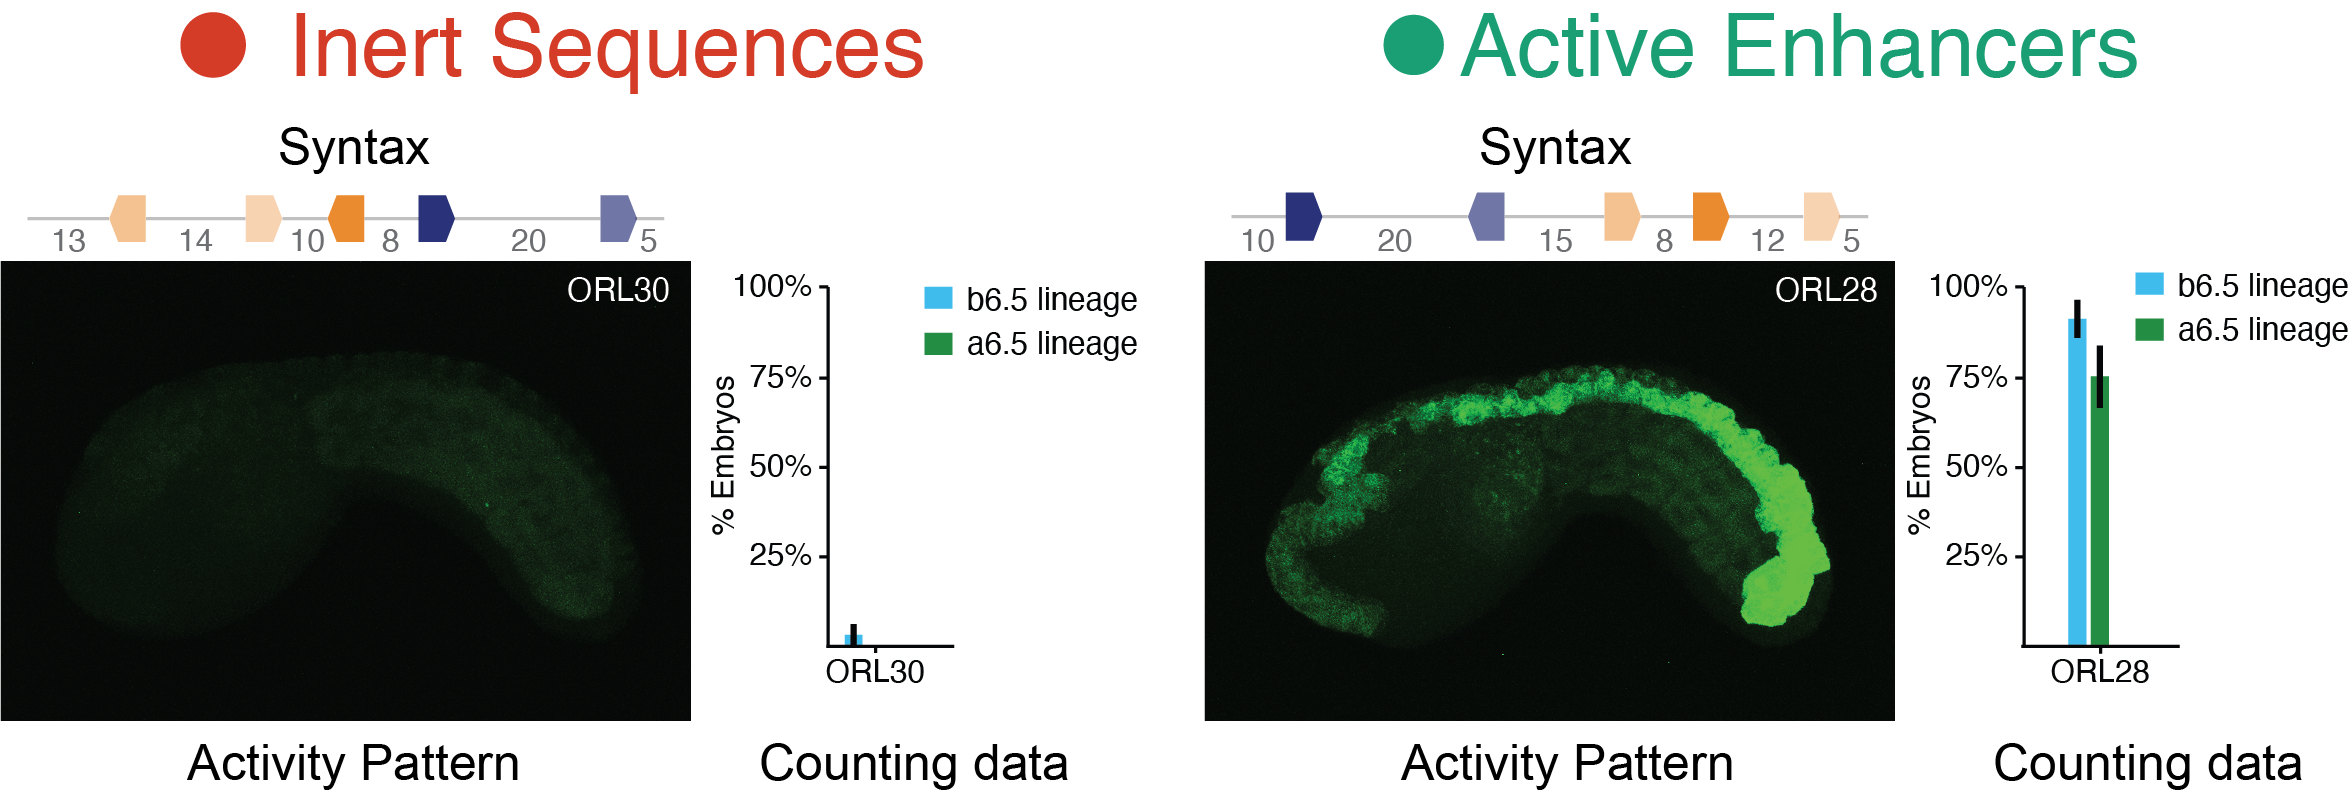
\includegraphics[width=0.85\textwidth]{2_figures-and-files/SuppFig3.png}
    \caption[Examples of microscope validated classification labels of library elements.]{\textbf{Examples of microscope validated classification labels of library elements.} 23 OSL elements were randomly selected for validation with fluorescence microscopy and classified as Inert Sequences or Active Enhancers based on counting data (\textbf{Figure~\ref{fig:2 Figure 1}g}). \textbf{Left,} example syntax with no expression classified as Inert Sequence. \textbf{Right,} example syntax with Otx-a WT like expression classified as Active Enhancer. Counting data for a6.5 and b6.5 lineage activity in 50 embryos is shown.}
    \label{fig:2 supplementary_3}
\end{figure}

\begin{figure}[p]
    \centering
    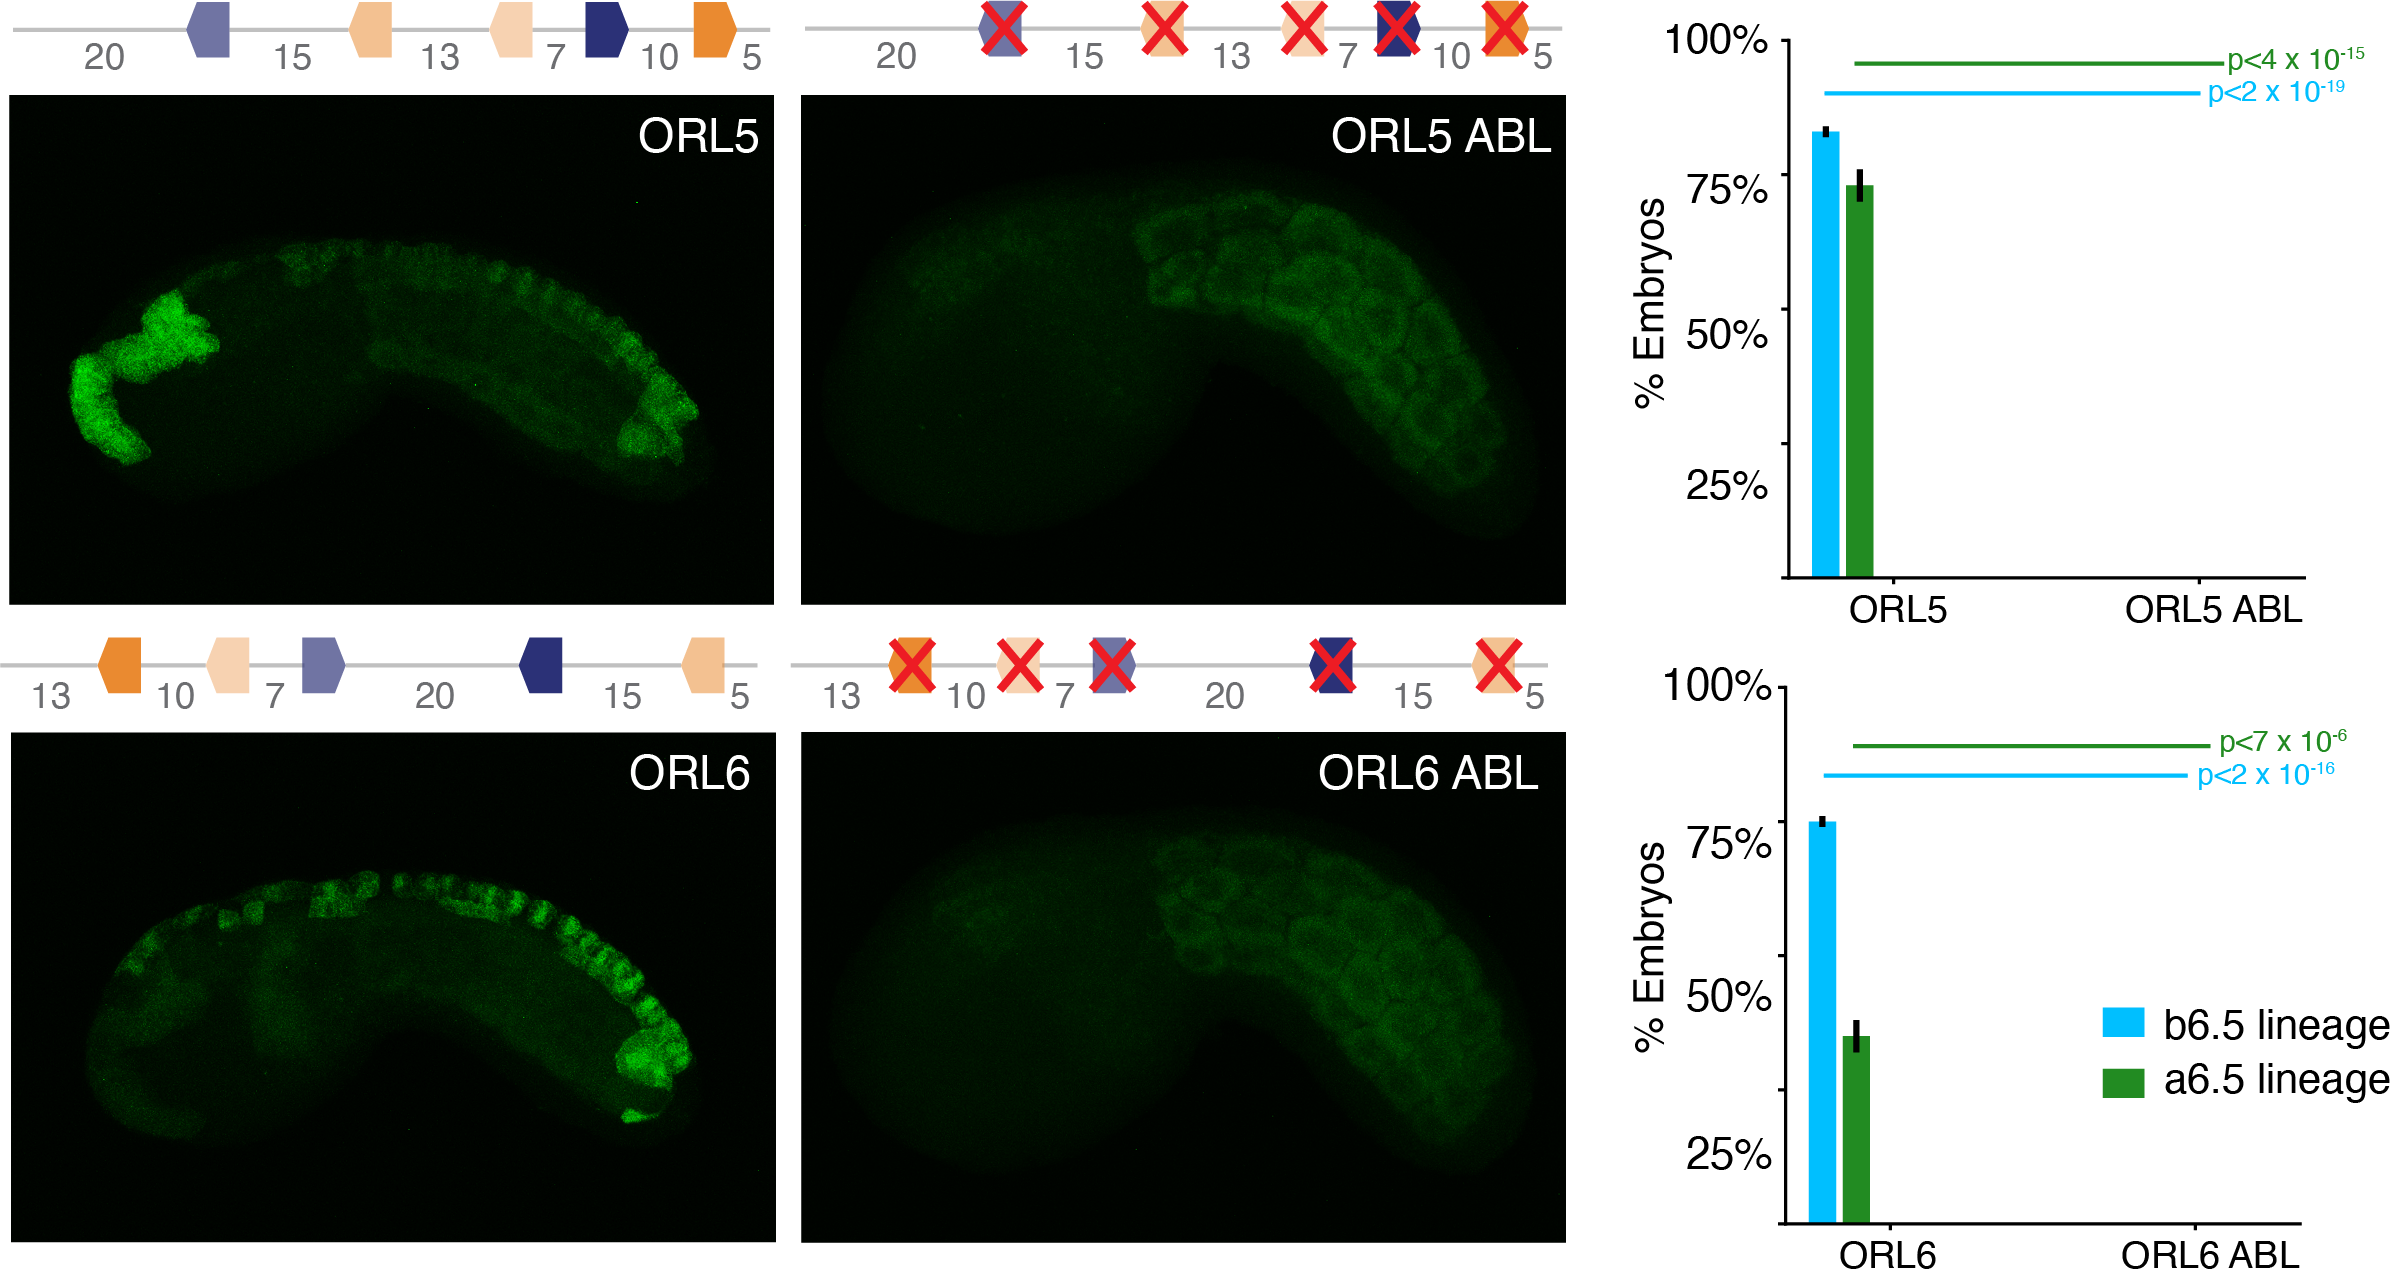
\includegraphics[width=0.9\textwidth]{2_figures-and-files/SuppFig4.png}
    \caption[GATA and ETS are required for neural expression of Otx-a scrambled elements.]{\textbf{GATA and ETS are required for neural expression of Otx-a scrambled elements.} \textbf{a)} OSL5 activates expression in the a6.5 and b6.5 lineages. \textbf{b)} OSL5 ABL construct in which all the GATA and ETS sites are ablated by point mutations (indicated with red Xs) activates no expression. \textbf{c)} Counting for OSL5 and OSL5 ABL shows \% of embryos with expression in the a6.5 and b6.5 lineages. 50 embryos counted in each replicate. \% embryos with expression is significantly different between OSL5 and OSL5 ABL (p < 4e-15 Fisher’s exact test, 2 replicates of 50 embryos each). \textbf{d)} OSL6 enhancer drives expression in the a6.5 and b6.5 lineage neural tissues. \textbf{e)} OSL6 ABL activates no expression. \textbf{f)} Counting data for OSL6 and OSL6 ABL shows \% of embryos with expression in the a6.5 and b6.5 lineages. 50 embryos counted in each replicate. \% embryos with expression is significantly different between OSL6 and OSL6 ABL (p < 4e-15 Fisher’s exact test, 2 replicates of 50 embryos each).}
    \label{fig:2 supplementary_4}
\end{figure}

\begin{figure}[p]
    \centering
    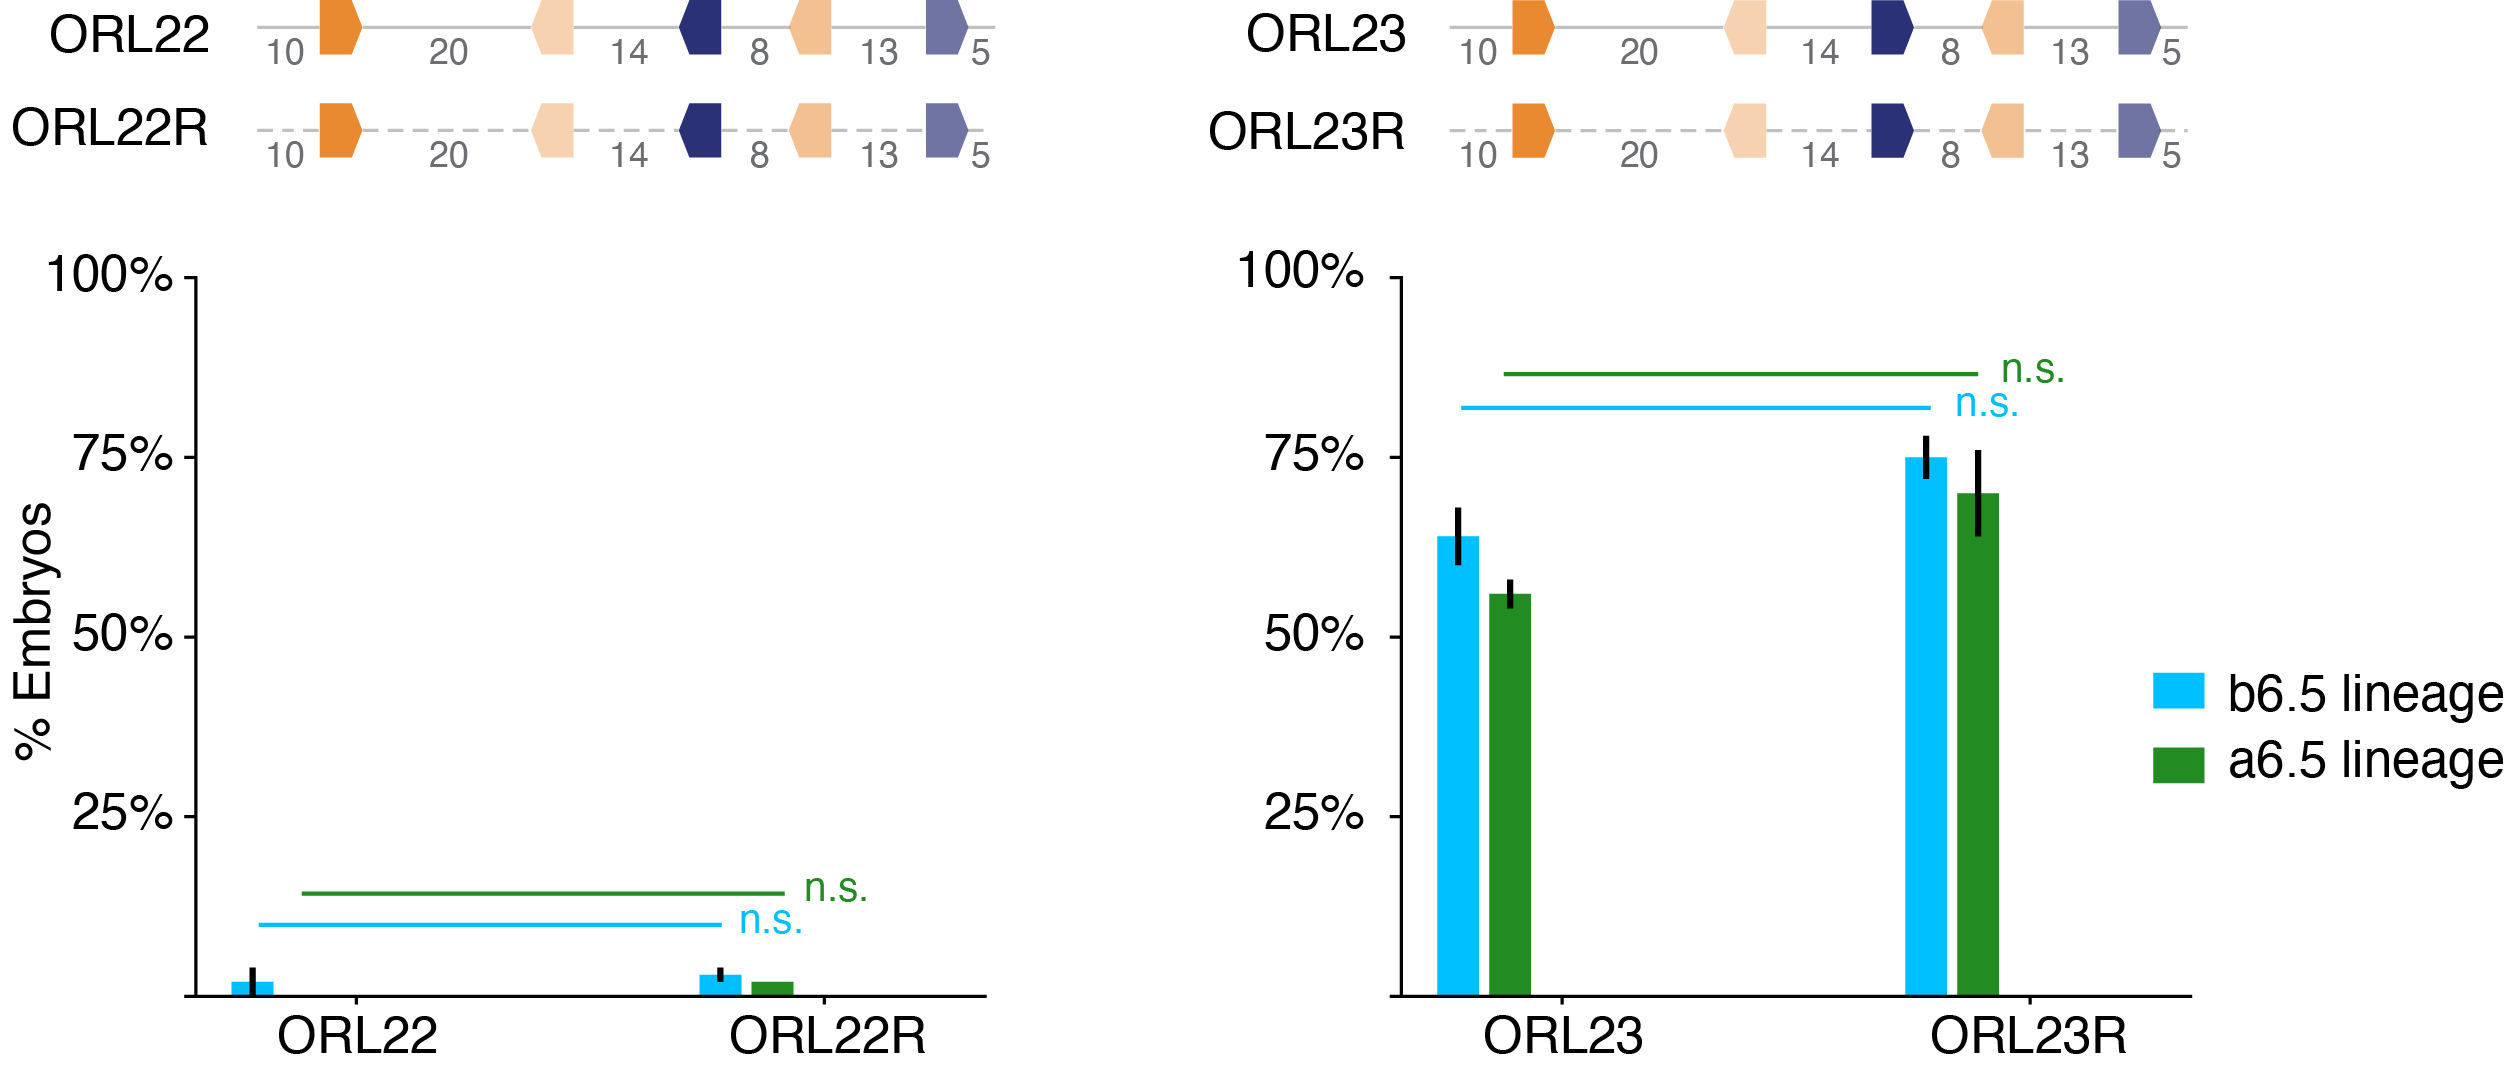
\includegraphics[width=0.85\textwidth]{2_figures-and-files/SuppFig5.png}
    \caption[Organization of binding sites matters for encoding active enhancers.]{\textbf{Organization of binding sites matters for encoding active enhancers.} \textbf{a)} In the randomized construct OSL22R, all bases of the linker sequences are replaced with N nucleotides which represent an equal chance of A, T, G or C. More than 3 million unique sequences in the OSL22R library. OSL22 and OSL22R have no significant difference in percent embryos with expression in either a6.5 or b6.5 lineages (Fisher’s exact test, two replicates of 50 embryos each). \textbf{b)} OSL23 is an element activating expression in a6.5 and b6.5 neural tissues. OSL23R with randomized linker sequences, comprising over 3 million unique sequences, is not significantly different from OSL23 in change in percent embryos with expression (Fisher’s exact test, two replicates of 50 embryos each).}
    \label{fig:2 supplementary_5}
\end{figure}

\begin{figure}[p]
    \centering
    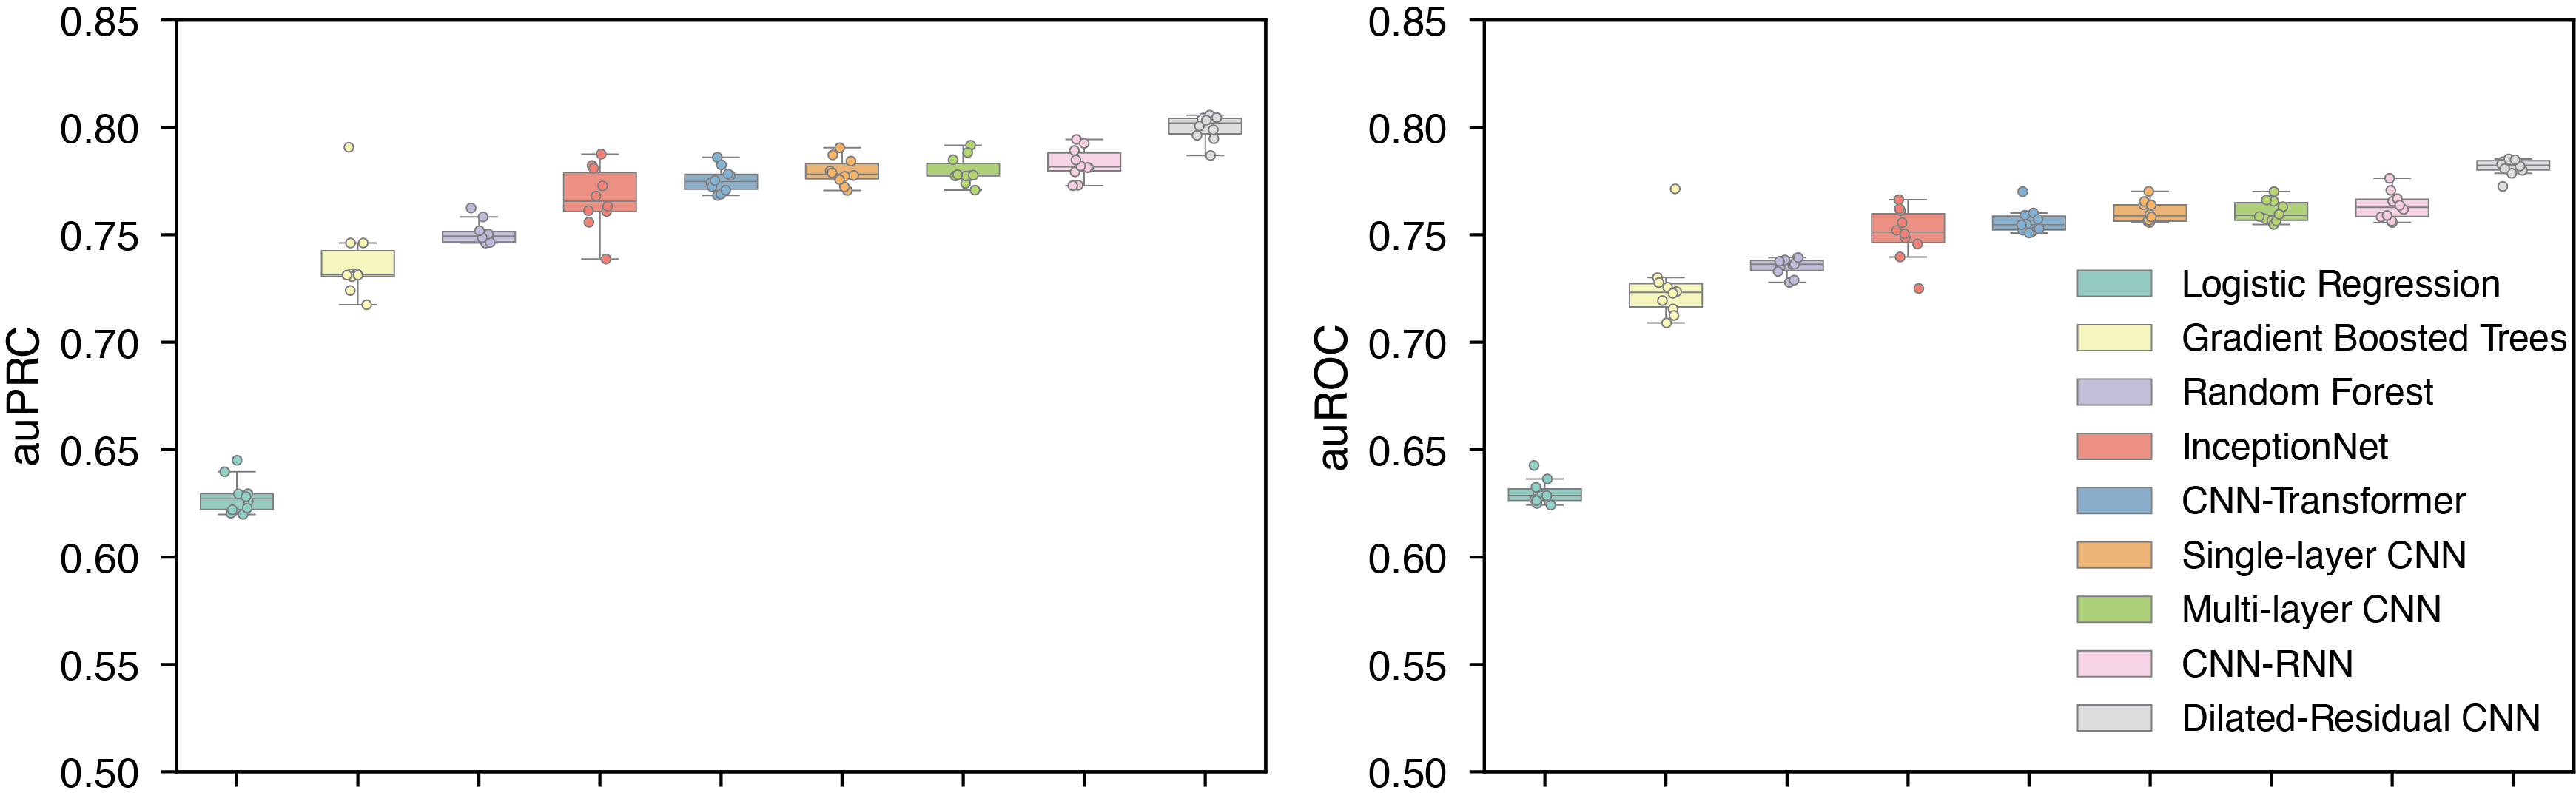
\includegraphics[width=0.85\textwidth]{2_figures-and-files/SuppFig6.png}
    \caption[10-fold cross validation performance of syntax models.]{\textbf{10-fold cross validation performance of syntax models.} 10-fold cross validation area under the precision-recall curve (auPRC, left) and area under the receiver operating characteristic curve (auROC, right) for several classes of machine learning model. The box plots show distributions for each performance metric and each point represents the performance on an individual fold of the data. The boxes show medians along with low and high quartiles. Whiskers extend to the furthest datapoint within 1.5-times the interquartile range. More extreme points are marked as outliers.}
    \label{fig:2 supplementary_6}
\end{figure}

\begin{figure}[p]
    \centering
    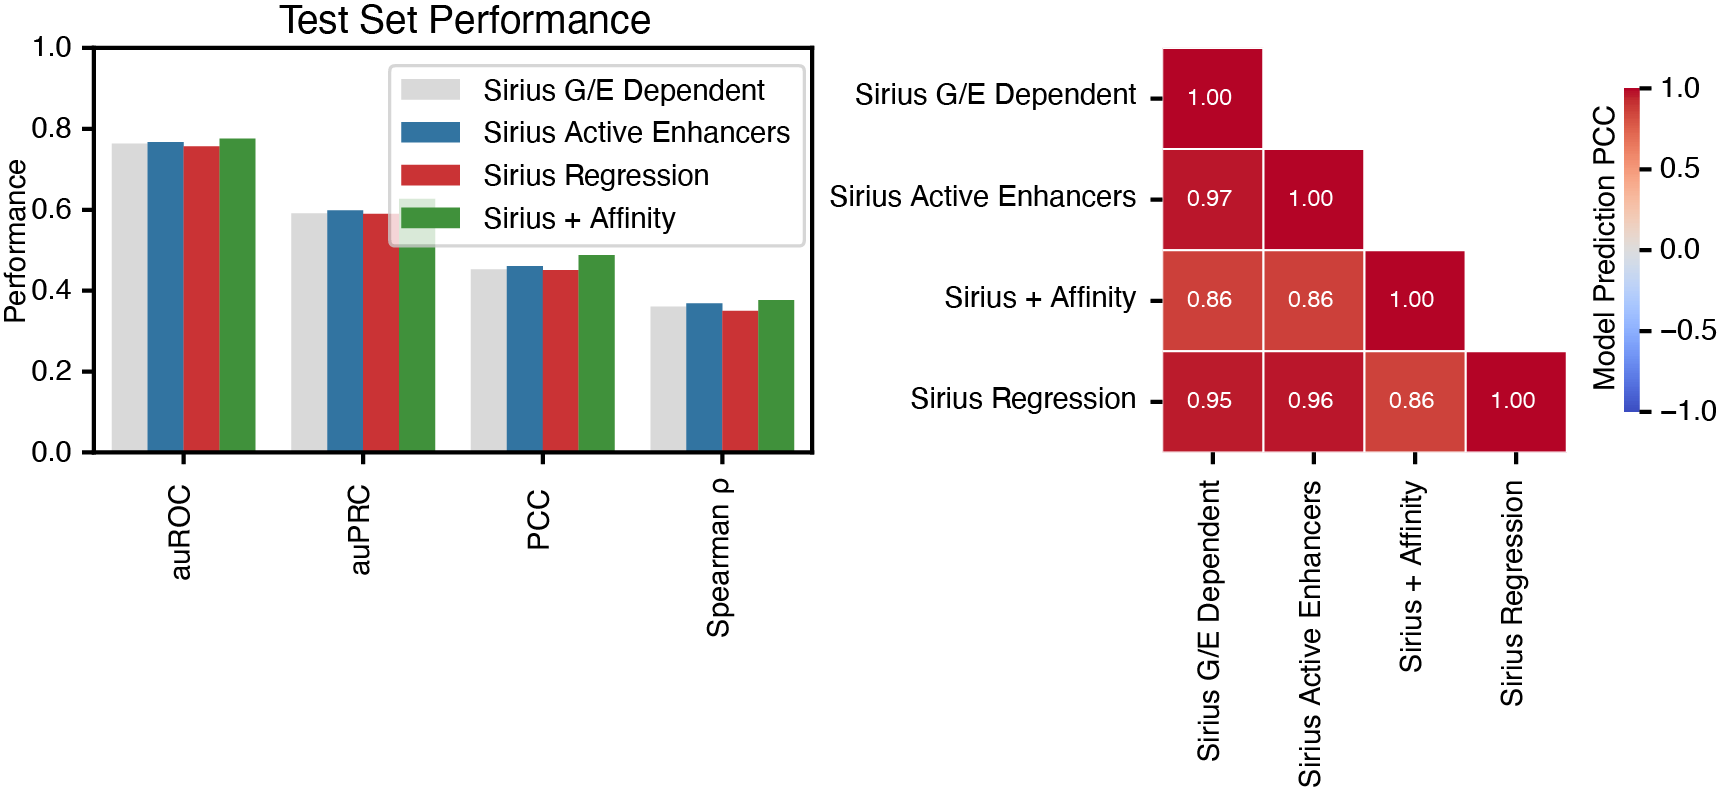
\includegraphics[width=0.85\textwidth]{2_figures-and-files/SuppFig7.png}
    \caption[Sirius predictions are robust to different training strategies.]{\textbf{Sirius predictions are robust to different training strategies.} \textbf{a)} Comparison of different training strategies across four performance metrics: area under the receiver operator characteristic curve (auROC), area under the precision-recall curve (auPRC), Pearson correlation coefficient (PCC), and Spearman’s $rho$. \textbf{b)} Heatmap shows pairwise PCC of test-set predictions for each model type (see Methods). Briefly, Sirius G/E Dependent refers to Sirius models trained on active enhancers driven by GATA and ETS sites (N=52,139). Sirius Active Enhancers refers to Sirius models trained on all active enhancers (N=80,965). Sirius Regression refers to models trained to predict the quantitative enhancer activity level using all detected sequences (N=393,554). Sirius + Affinity are trained on active enhancers driven by GATA and ETS sites, but use separate channels for each GATA affinity (G1, G2, and G3) and each ETS affinity (E1 and E2).}
    \label{fig:2 supplementary_7}
\end{figure}

\begin{figure}[p]
    \centering
    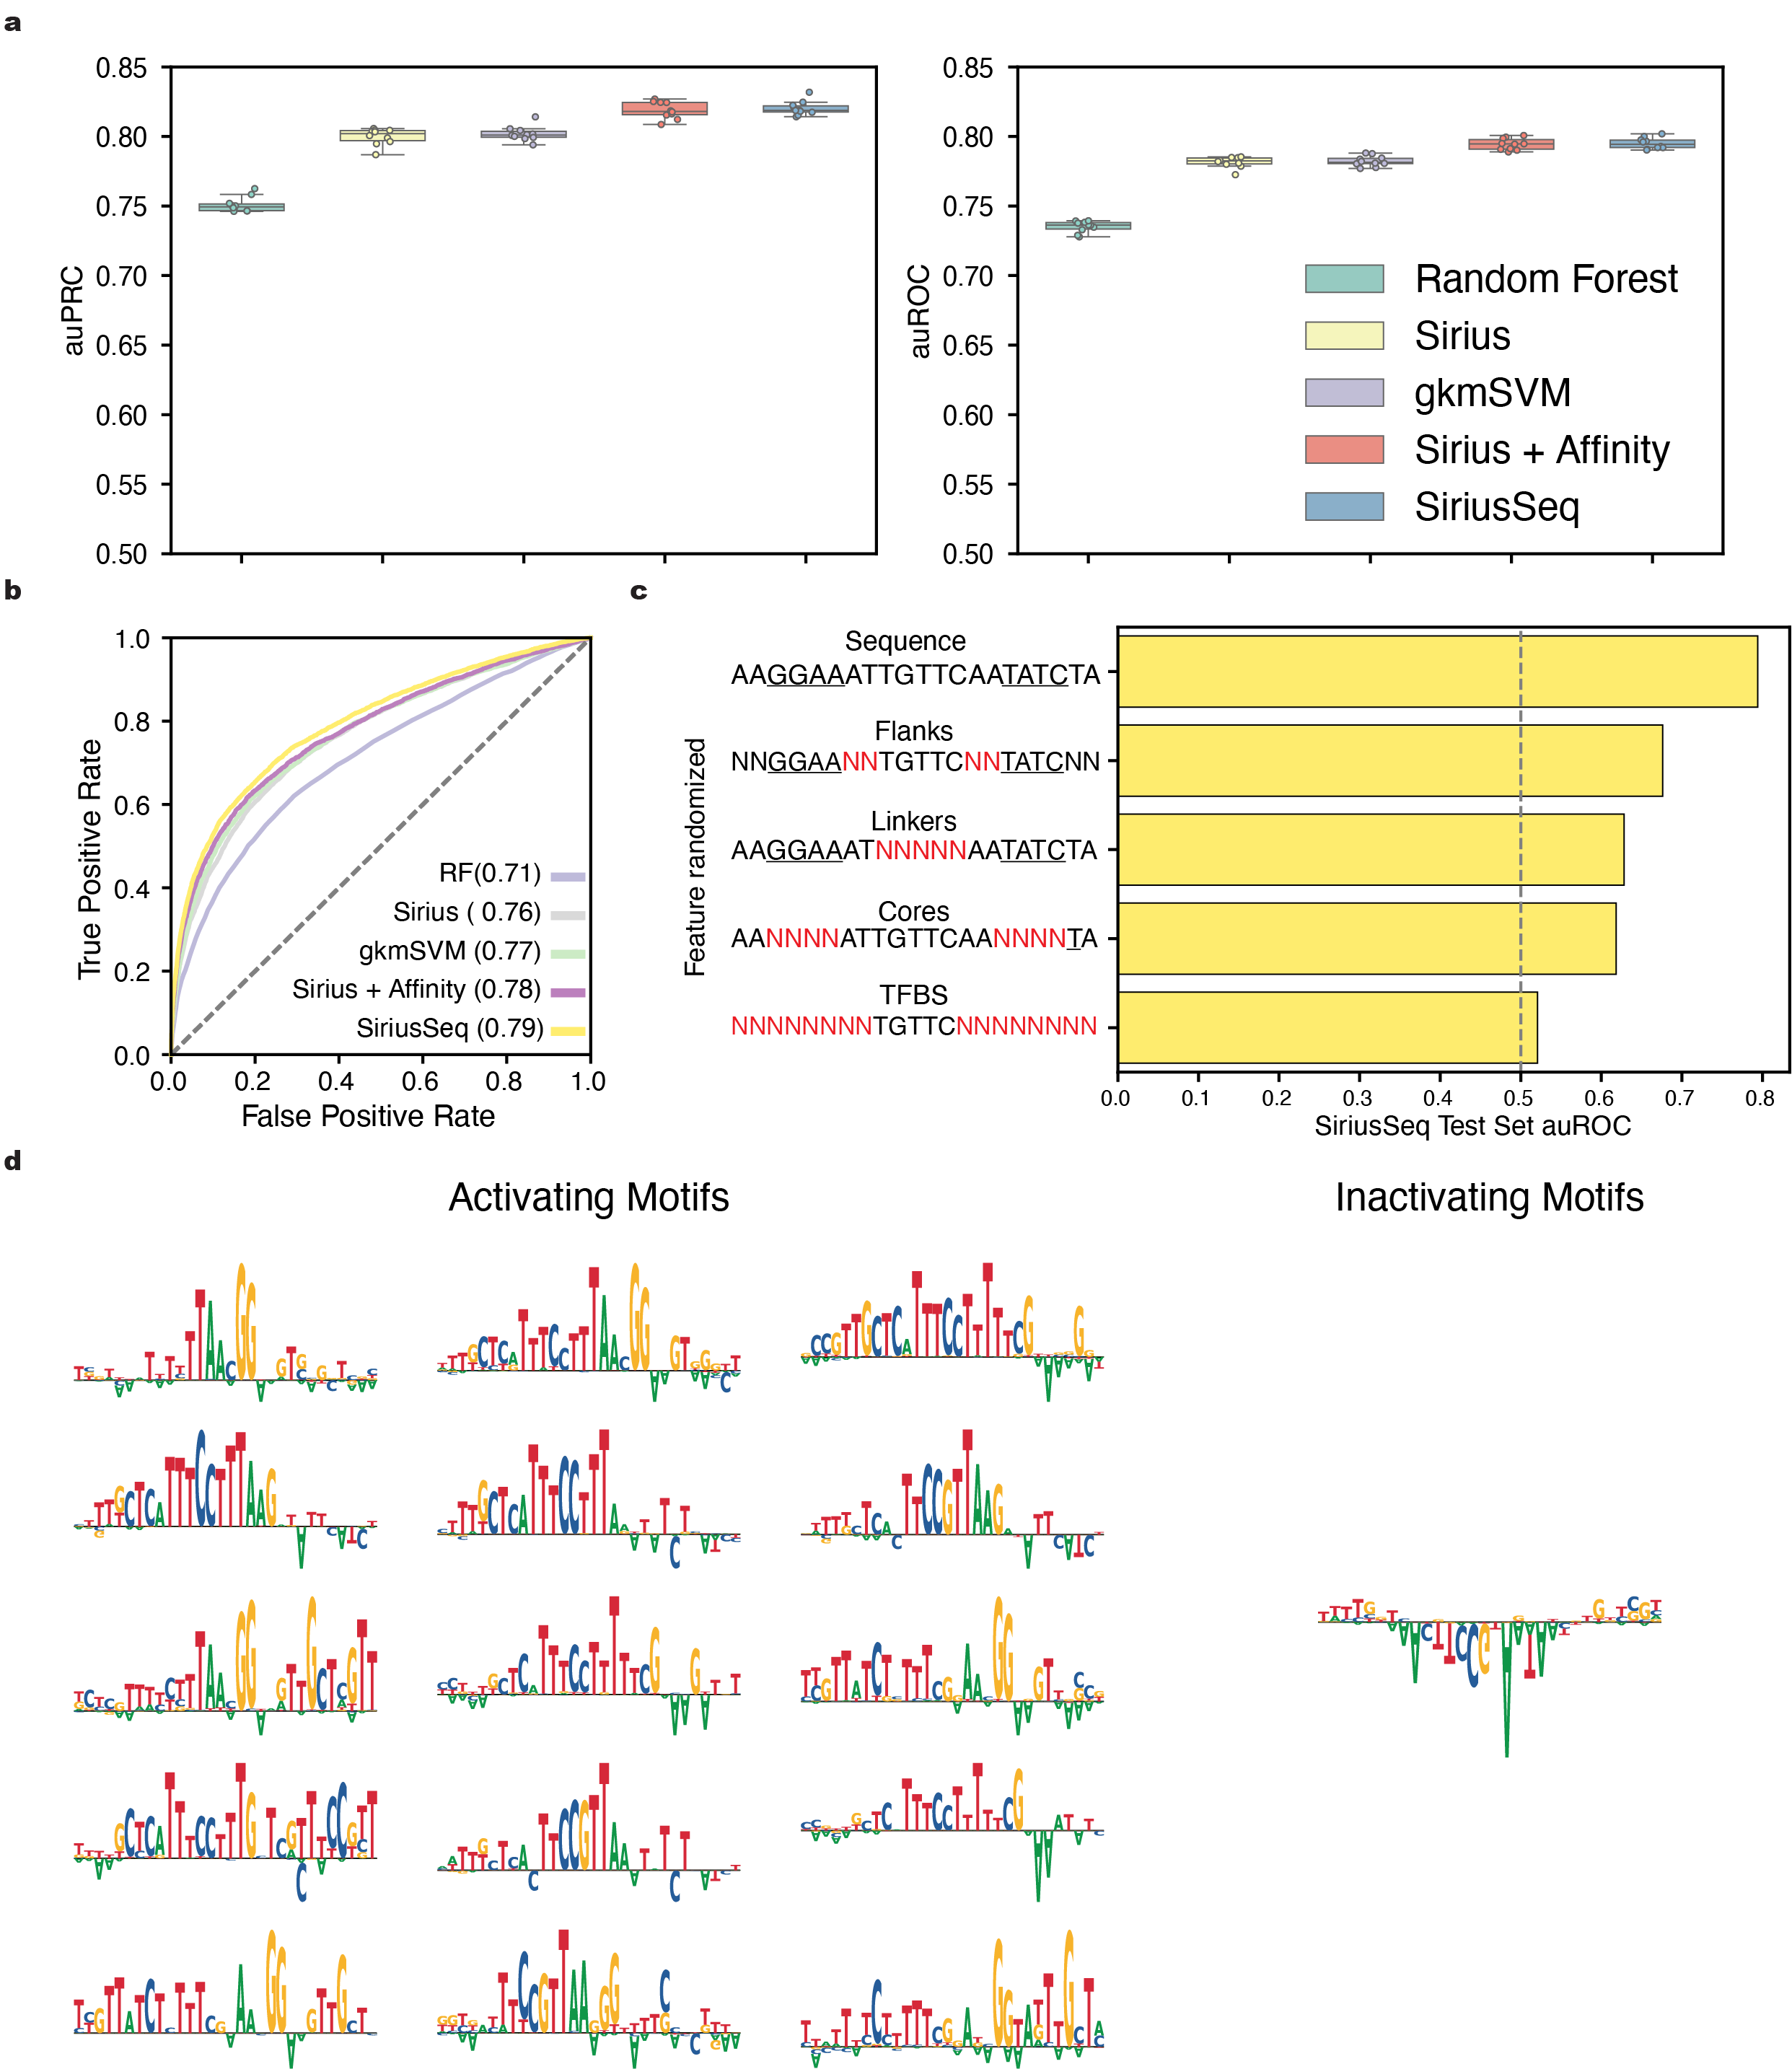
\includegraphics[width=0.85\textwidth]{2_figures-and-files/SuppFig8.png}
    \caption[Models trained on linear DNA sequence learn non-syntax features that marginally contribute to predictive performance.]{\textbf{Models trained on linear DNA sequence learn non-syntax features that marginally contribute to predictive performance.} \textbf{a)} 10-fold cross validation auPRC (left) and auROC (right) for several classes of machine learning model. The box plots show distributions for each performance metric and each point represents the performance on an individual fold of the data. The boxes show medians along with low and high quartiles. Whiskers extend to the furthest datapoint within 1.5-times the interquartile range. More extreme points are marked as outliers. \textbf{b)} Receiver operator characteristic curves for the same models as in \textbf{a)}. \textbf{c)} SiriusSeq held-out test set auROCs on sequences with the indicated randomized features. \textbf{d)} TF-MoDISco discovered motifs from SiriusSeq split into activating and inactivating motifs.}
    \label{fig:2 supplementary_8}
\end{figure}

\begin{figure}[p]
    \centering
    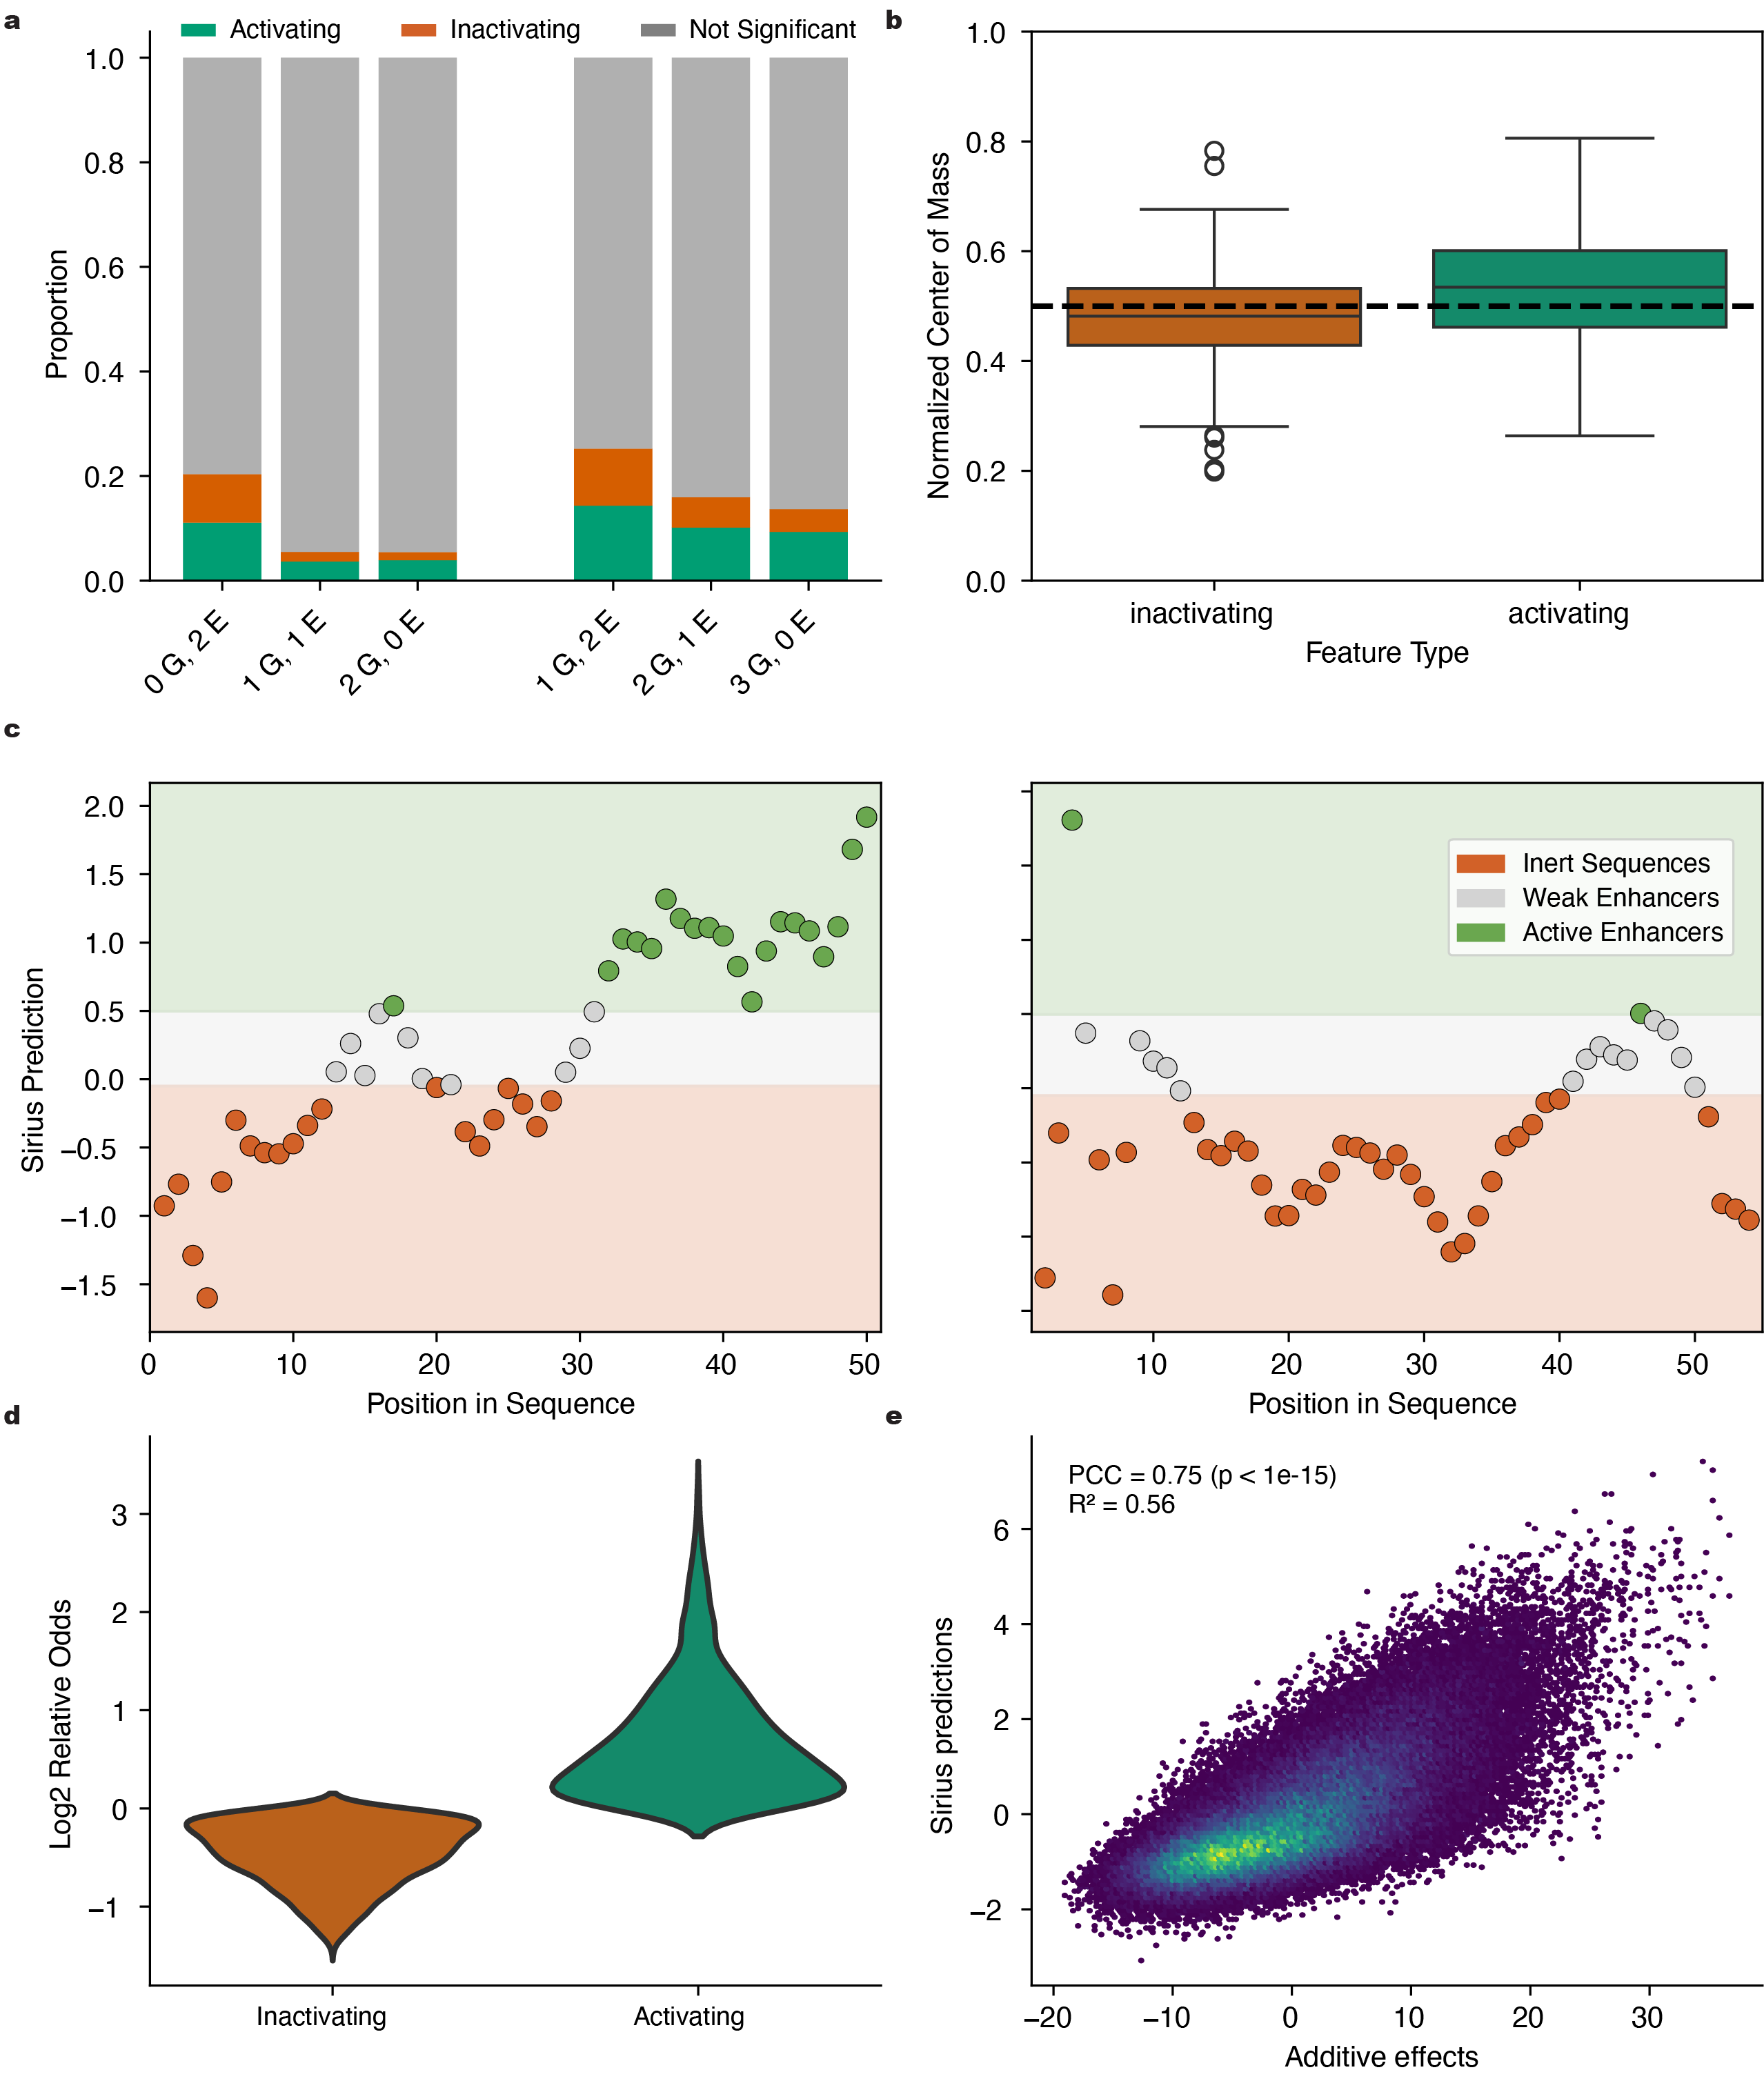
\includegraphics[width=0.85\textwidth]{2_figures-and-files/SuppFig9.png}
    \caption[Syntax feature analysis.]{\textbf{Syntax feature analysis.} \textbf{a)} Barplots of proportion of 2-site (left) and 3-site (right) syntax features split by possible combinations of ETS (E) and GATA (G) sites. P-values for Chi2 tests are 3.84e-05 and 3.06e-29 for 2-site and 3-site features respectively. \textbf{b)} Distributions for normalized center of mass of model predictions (y-axis) for inactivating and activating syntax features (see Methods). \textbf{c)} Examples of two 2-site features exhibiting periodic positional preferences. Y-axis represents Sirius predictions for syntax features across possible positions (x-axis). \textbf{Left,} g.10.E. \textbf{Right,} E.7.G. Background colors are determined by the interquartile ranges of the active enhancers and inert sequences in the OSL library. The range in between the upper quartile of the inert sequences and the lower quartile of the active enhancers is classified as weak enhancers. \textbf{d)} 2,494 single syntax changes flip a 3-site syntax feature from a negative Log2 relative mean odds (inactivating) to a positive one (activating). \textbf{e)} Scatterplot of predictions for AdditiveFeatures (x-axis) against Sirius (y-axis). Pearson correlation coefficient (PCC) and percent variance explained (R²) are annotated in the top left.}
    \label{fig:2 supplementary_9}
\end{figure}

\begin{figure}[p]
    \centering
    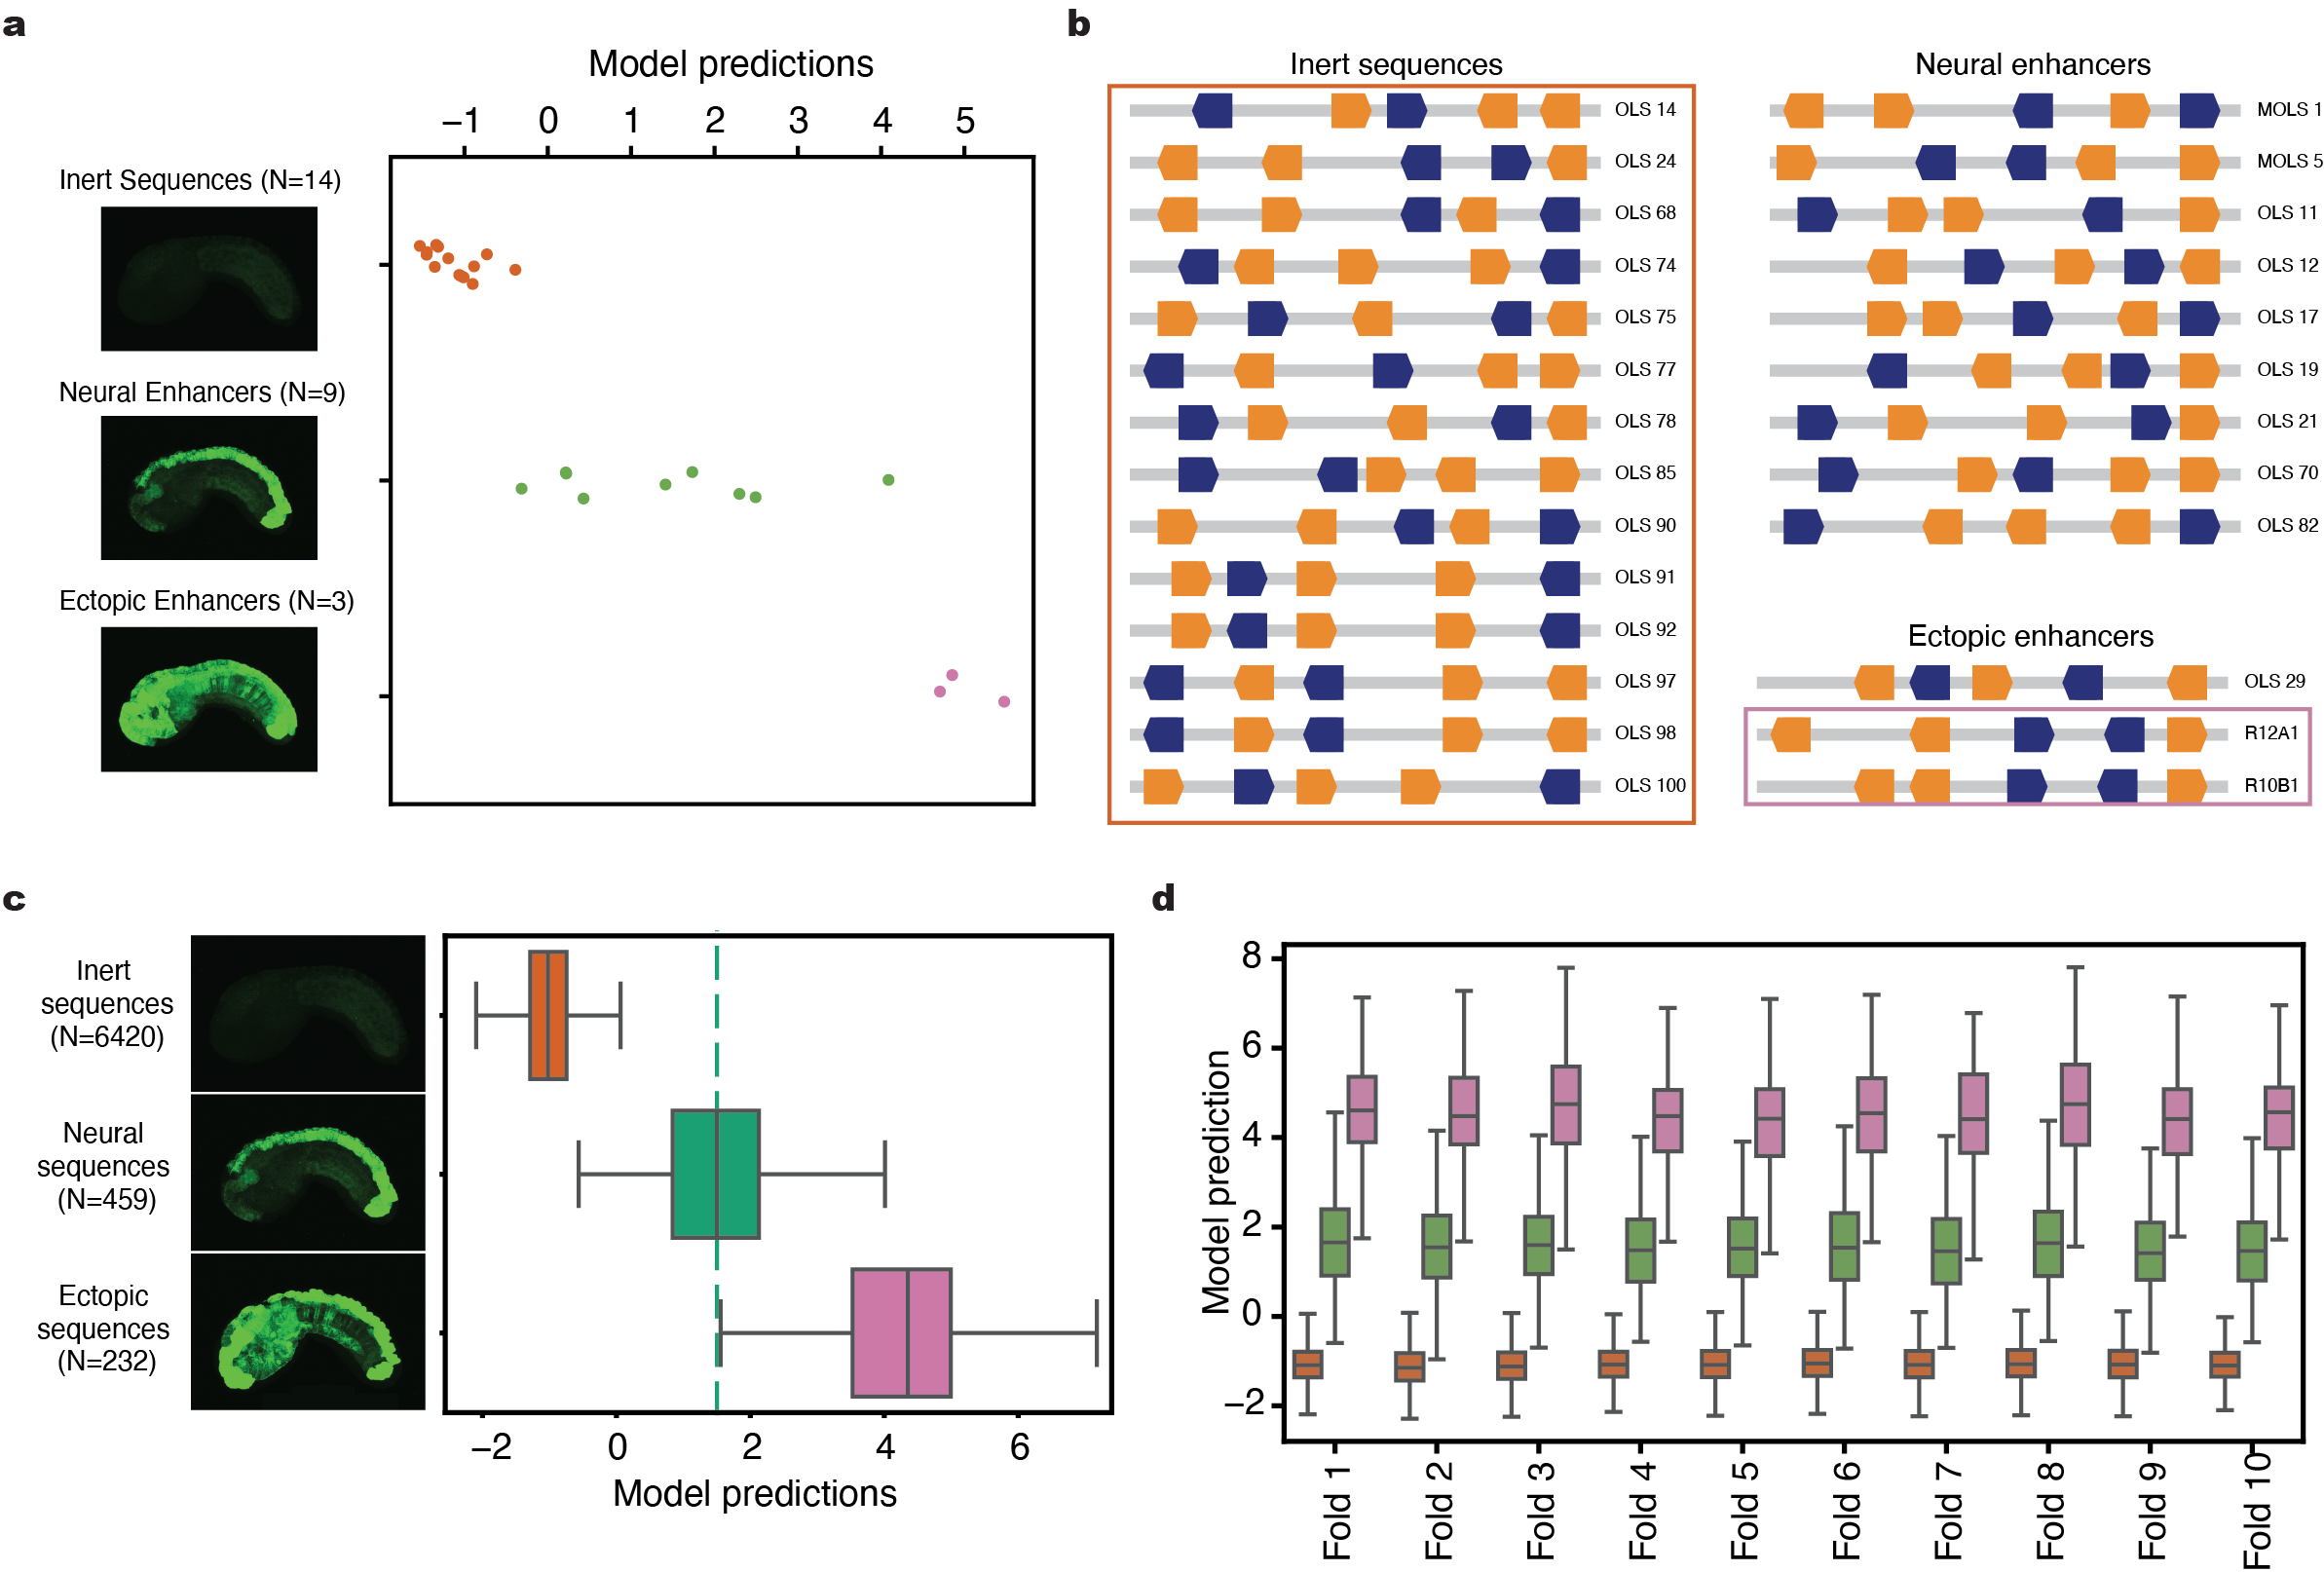
\includegraphics[width=0.9\textwidth]{2_figures-and-files/SuppFig10.png}
    \caption[Sirius predictions show implicit tissue specificity.]{\textbf{Sirius predictions show implicit tissue specificity.} \textbf{a)} Model predictions (x-axis) across validated sequences binned by tissue specificity. \textbf{b)} Syntaxes for each point in \textbf{a)} binned by tissue specificity. Colored boxes around syntaxes indicate these were used in STARS design (\textbf{Figure~\ref{fig:2 Figure 4}}). \textbf{c)} Model predictions (x-axis) across OSL sequences binned by tissue specificity (see Methods). Representative fluorescence microscopy images are shown for each bin. The green dashed line indicates the median model prediction for neural sequences targeted during STARS design (\textbf{Figure~\ref{fig:2 Figure 4}}). \textbf{d)} Model predictions (y-axis) for OSL sequences binned by tissue specificity (see Methods) for all folds of cross-validation (x-axis).}
    \label{fig:2 supplementary_10}
\end{figure}

\begin{figure}[p]
    \centering
    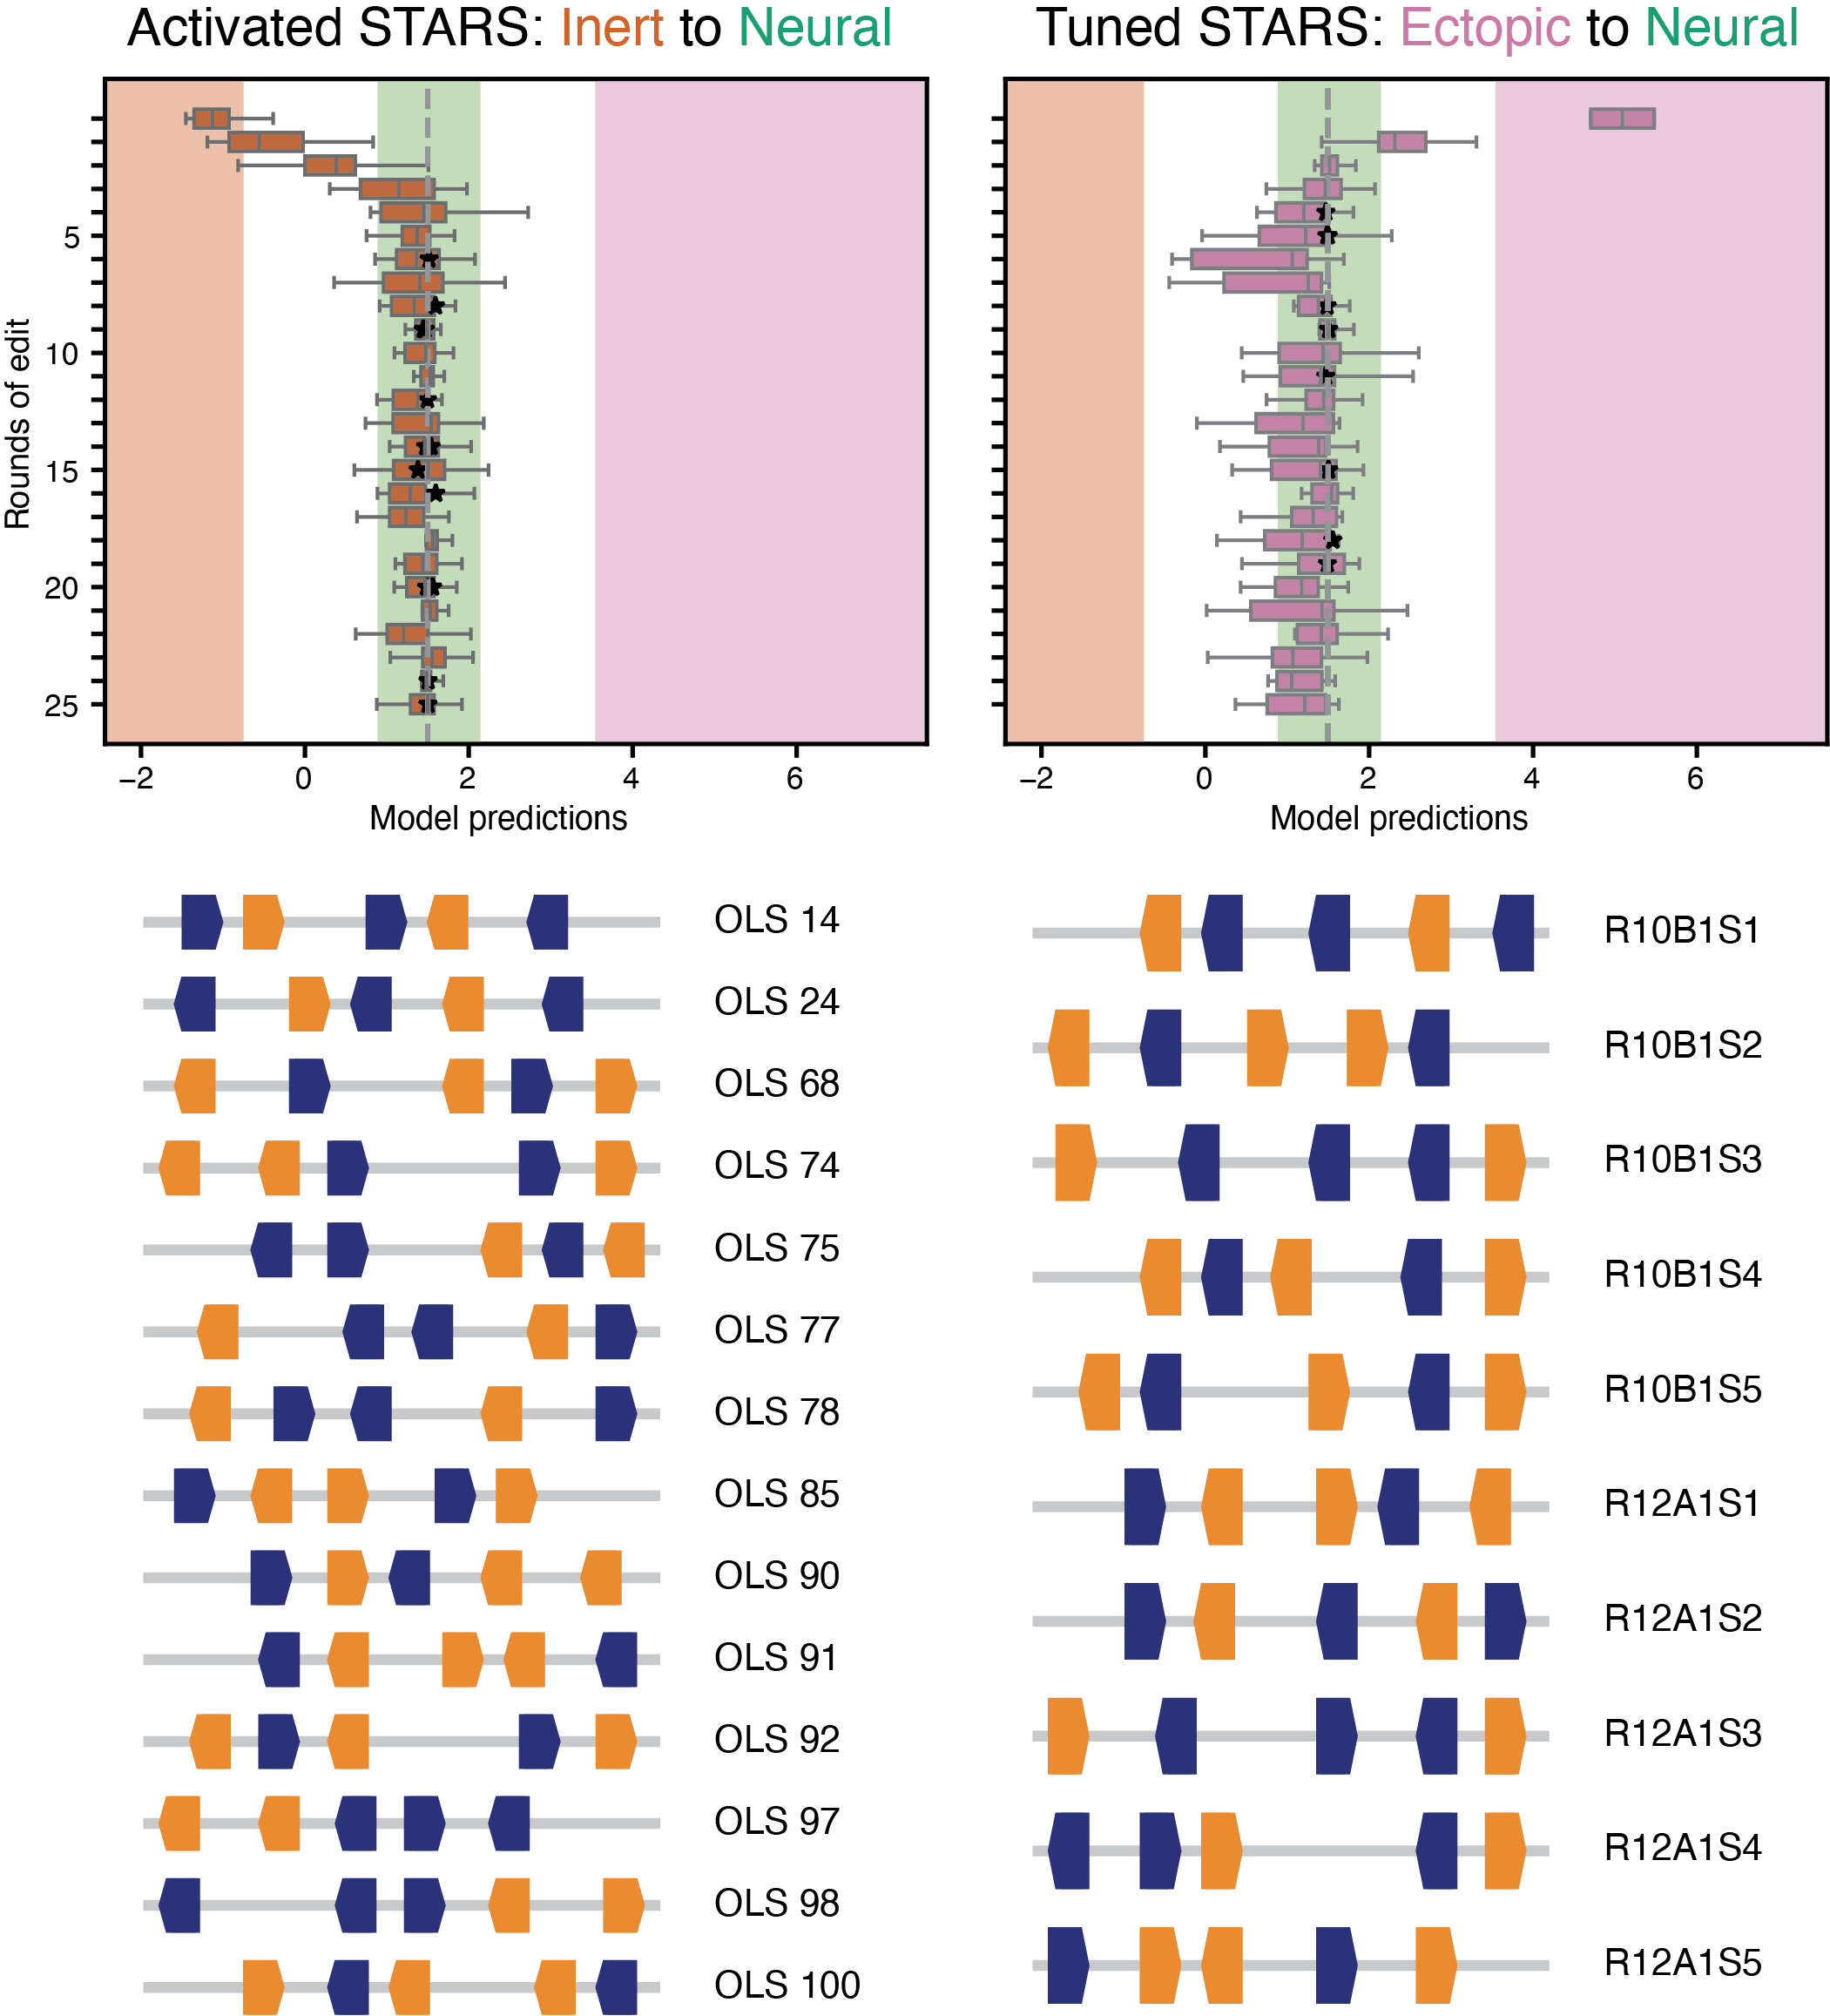
\includegraphics[width=0.88\textwidth]{2_figures-and-files/SuppFig11.png}
    \caption[24 Syntax-derived, Tissue-specific, Active, Regulatory Sequences (STARS).]{\textbf{24 Syntax-derived, Tissue-specific, Active, Regulatory Sequences (STARS).} Model prediction for each round. Background colors are determined by the interquartile ranges of the active enhancers and inert sequences in the OSL library. The range in between the upper quartile of the inert sequences and the lower quartile of the active enhancers is classified as weak enhancers. \textbf{Left,} activated STARS – syntaxes that are validated Inert Sequences are edited to activate them to a predicted Neural Enhancer syntax. \textbf{Right,} tuned STARS – syntaxes that are validated Ectopic Enhancers are edited to tune them to a predicted Neural Enhancer syntax. \textbf{Bottom,} syntax schematics for all 24 STARS. None of these syntaxes are found in the OSL library and represent novel organizations of sites.}
    \label{fig:2 supplementary_11}
\end{figure}

\begin{figure}[p]
    \centering
    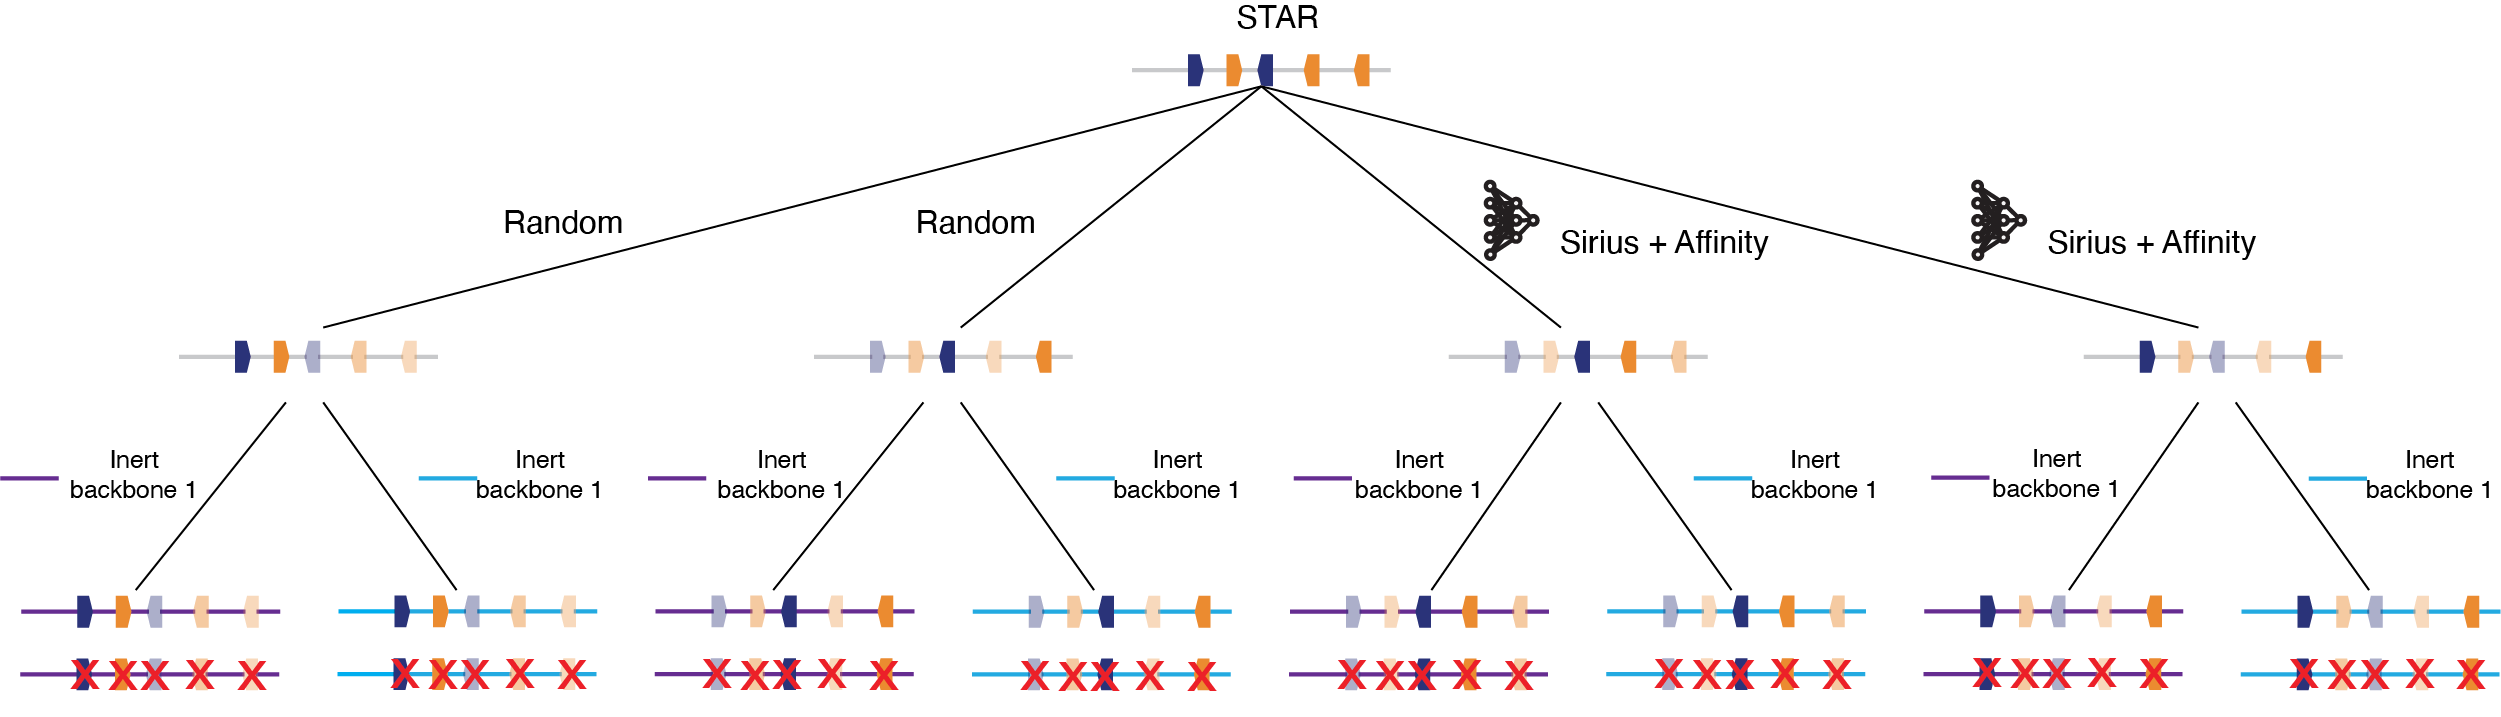
\includegraphics[width=0.88\textwidth]{2_figures-and-files/SuppFig12.png}
    \caption[STARS MPRA design.]{\textbf{STARS MPRA design.} Schematic for STARS library design and MPRA. For each of the 24 STARS, four different sets of flanking nucleotides were selected either randomly or with the Sirius + Affinity model. Two different sets of linker sequences were selected for each of the STARS from two different inert backbones. An ablated counterpart of each sequence was also synthesized where single point mutations within the core of each binding site that ablate binding of the TF are included.}
    \label{fig:2 supplementary_12}
\end{figure}

\begin{figure}[p]
    \centering
    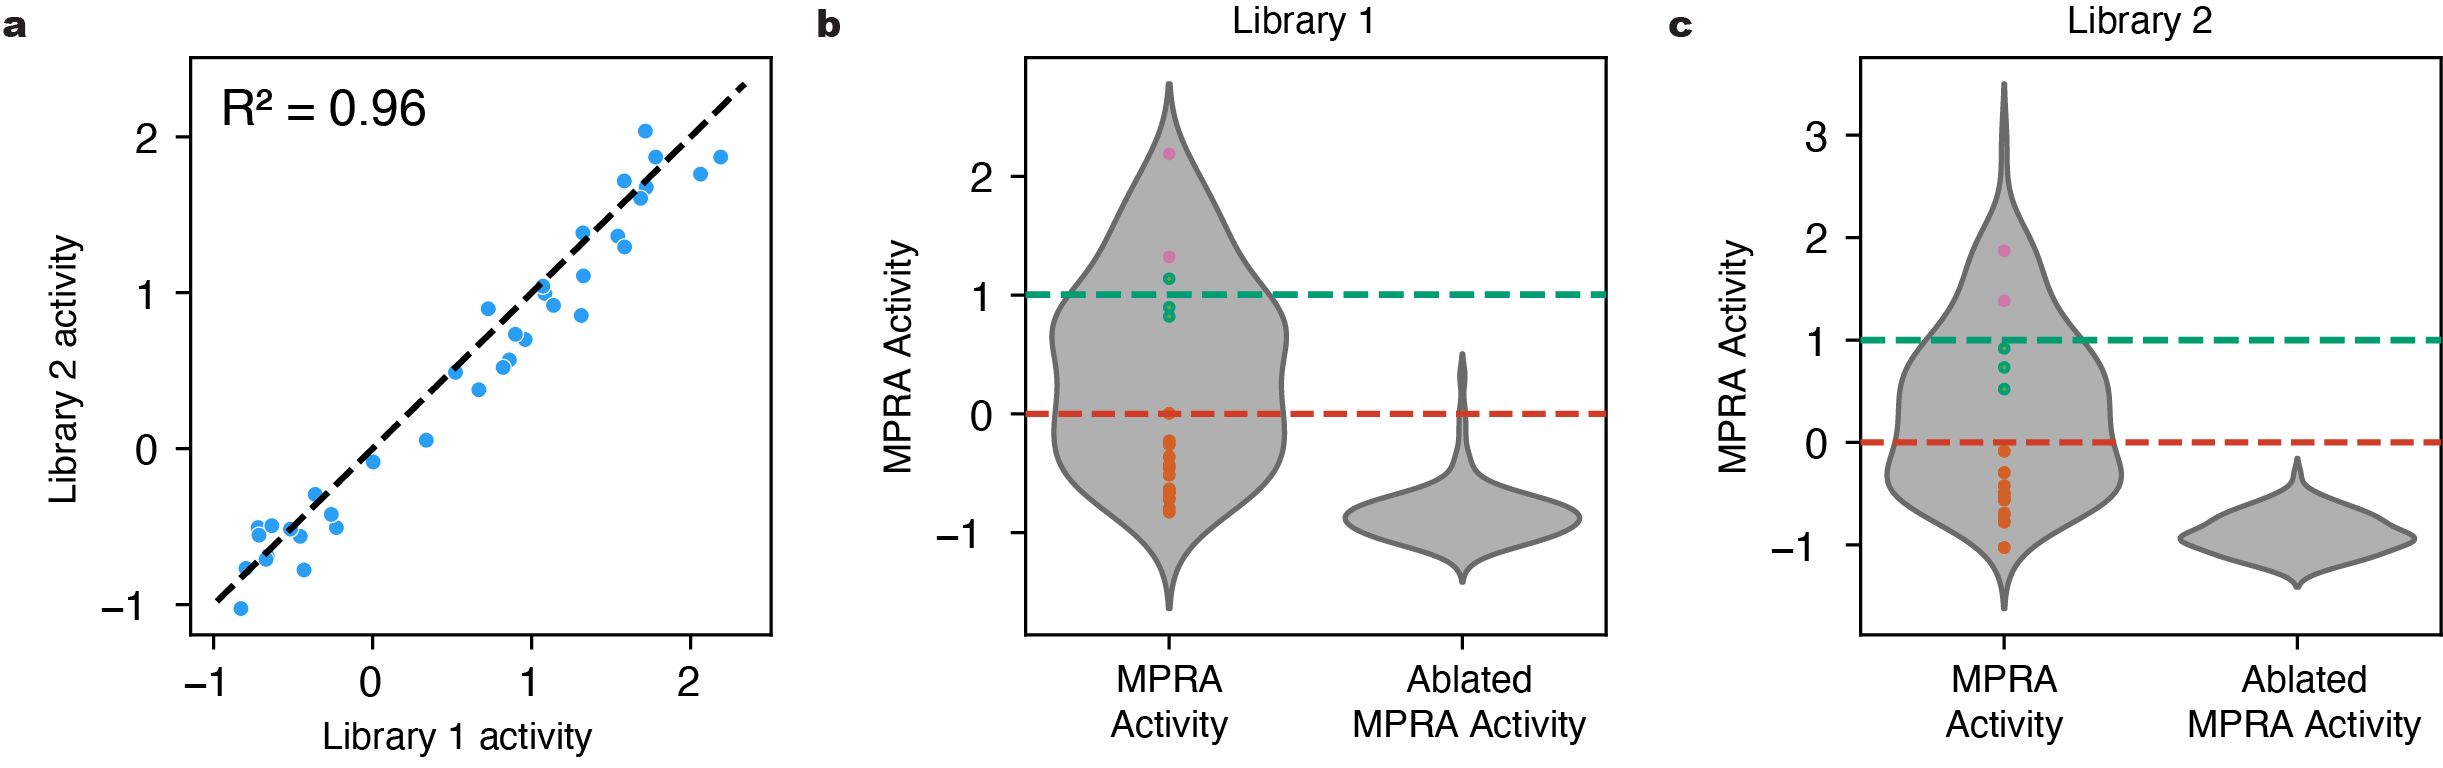
\includegraphics[width=0.88\textwidth]{2_figures-and-files/SuppFig13.png}
    \caption[Analysis of STARS MPRA.]{\textbf{Analysis of STARS MPRA.} \textbf{a)} Control reproducibility across STARS libraries. R² indicates the percentage of variance explained. \textbf{b)} Distributions of MPRA activities for library 1. \textbf{c)} Distributions of MPRA activities for library 2. The left violin for each subplot indicates the 96 WT elements tested and the right violin indicates the 96 ablated counterparts to those variants. Stripplot highlights validated controls that are inert sequences, neural enhancers and ectopic enhancers with horizontal dashed lines indicating thresholds used for classification.}
    \label{fig:2 supplementary_13}
\end{figure}

\begin{figure}[p]
    \centering
    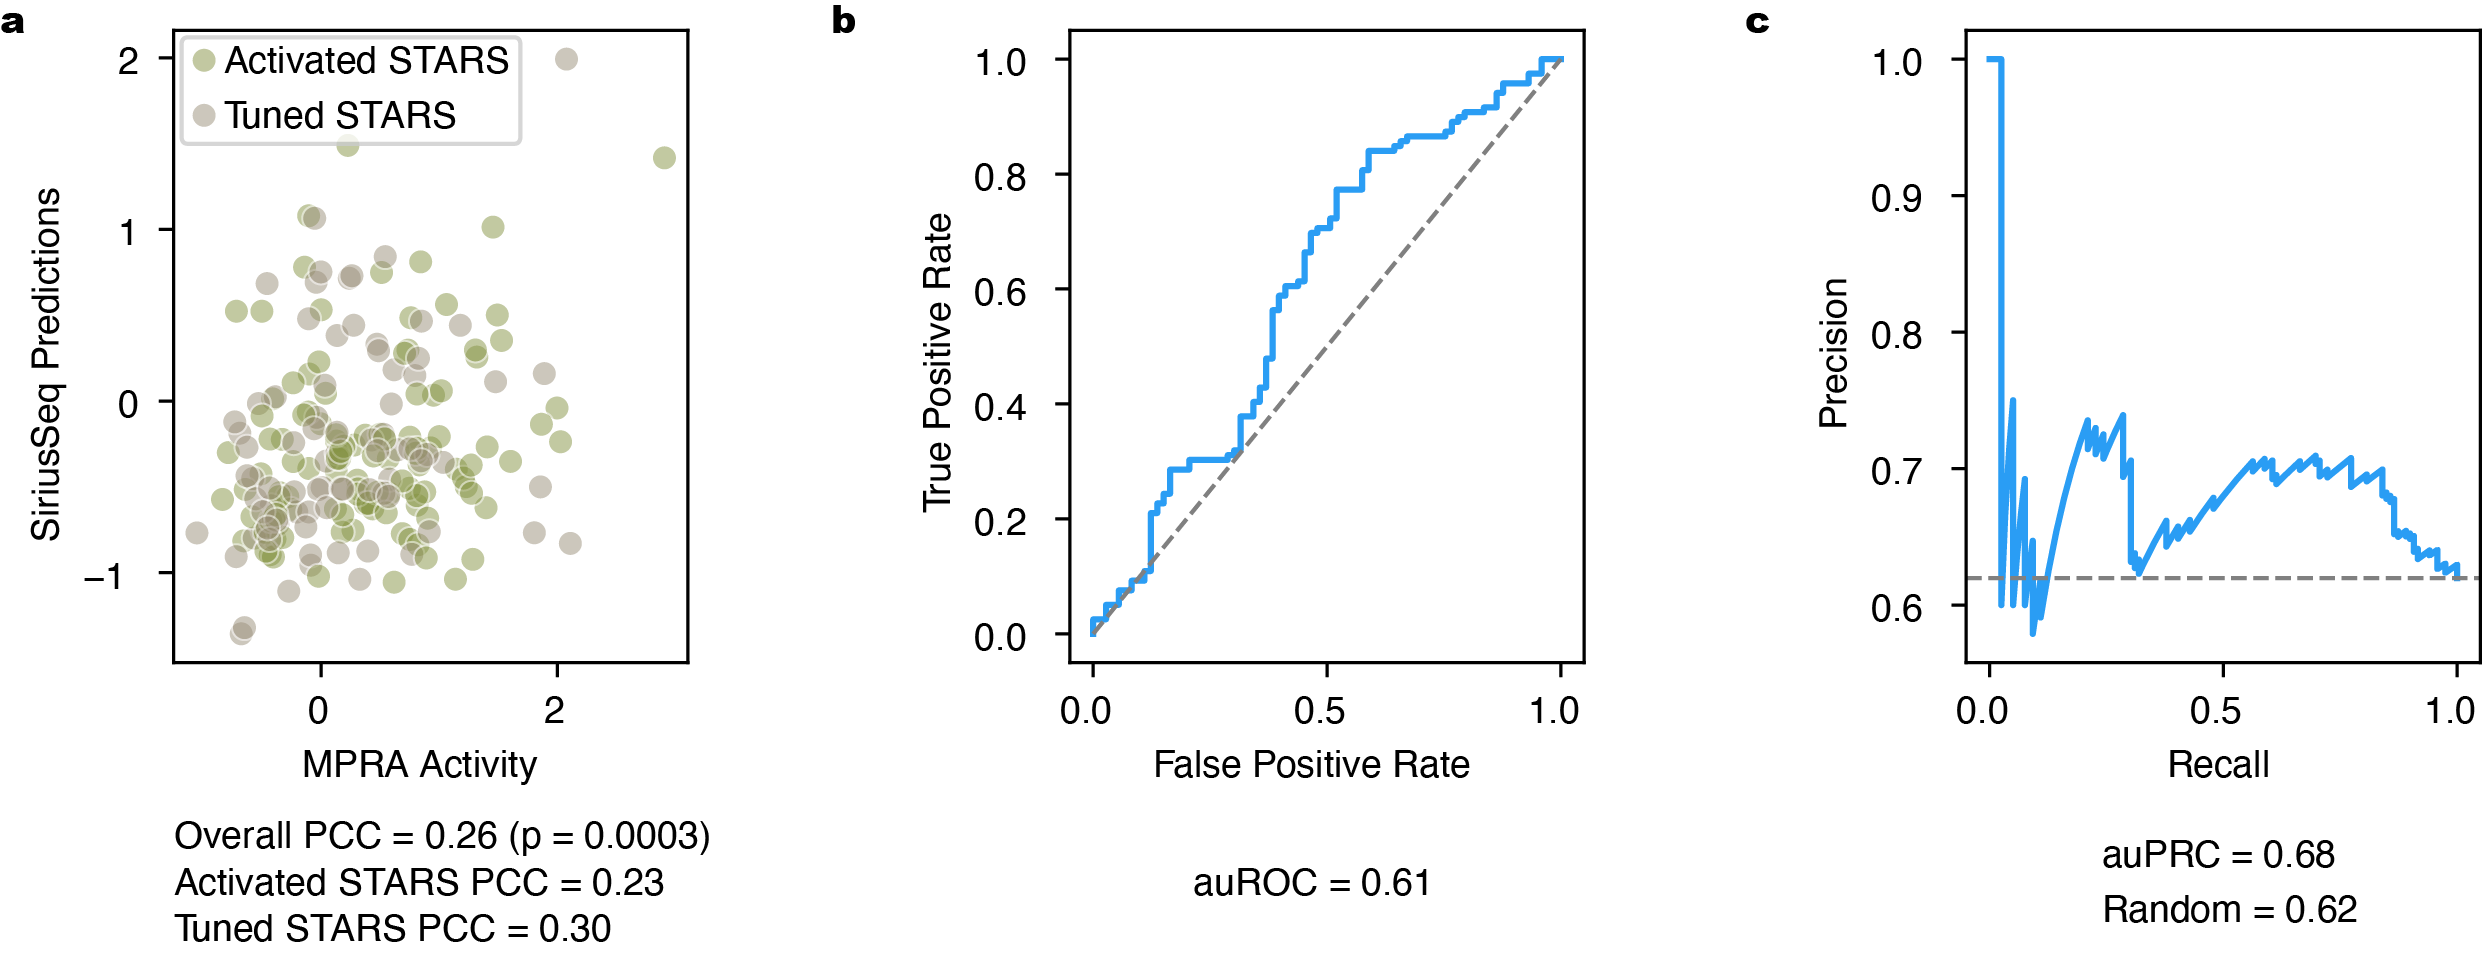
\includegraphics[width=0.88\textwidth]{2_figures-and-files/SuppFig14.png}
    \caption[SiriusSeq performance on STARS MPRA.]{\textbf{SiriusSeq performance on STARS MPRA.} \textbf{a)} Scatterplot of measured STARS MPRA activity (x-axis) against SiriusSeq predictions colored by direction of design. Pearson correlation coefficients (PCCs) for all designs and split by direction are shown below. \textbf{b)} Precision-recall and \textbf{c)} receiver operating characteristic curves for Sirius predictions on binarized activity (using controls, see \textbf{Figure~\ref{fig:2 supplementary_13}}). Area under the precision-recall curve (auPRC) and area under the receiver operating characteristic curve (auROC) are shown below the plots.}
    \label{fig:2 supplementary_14}
\end{figure}

\begin{figure}[p]
    \centering
    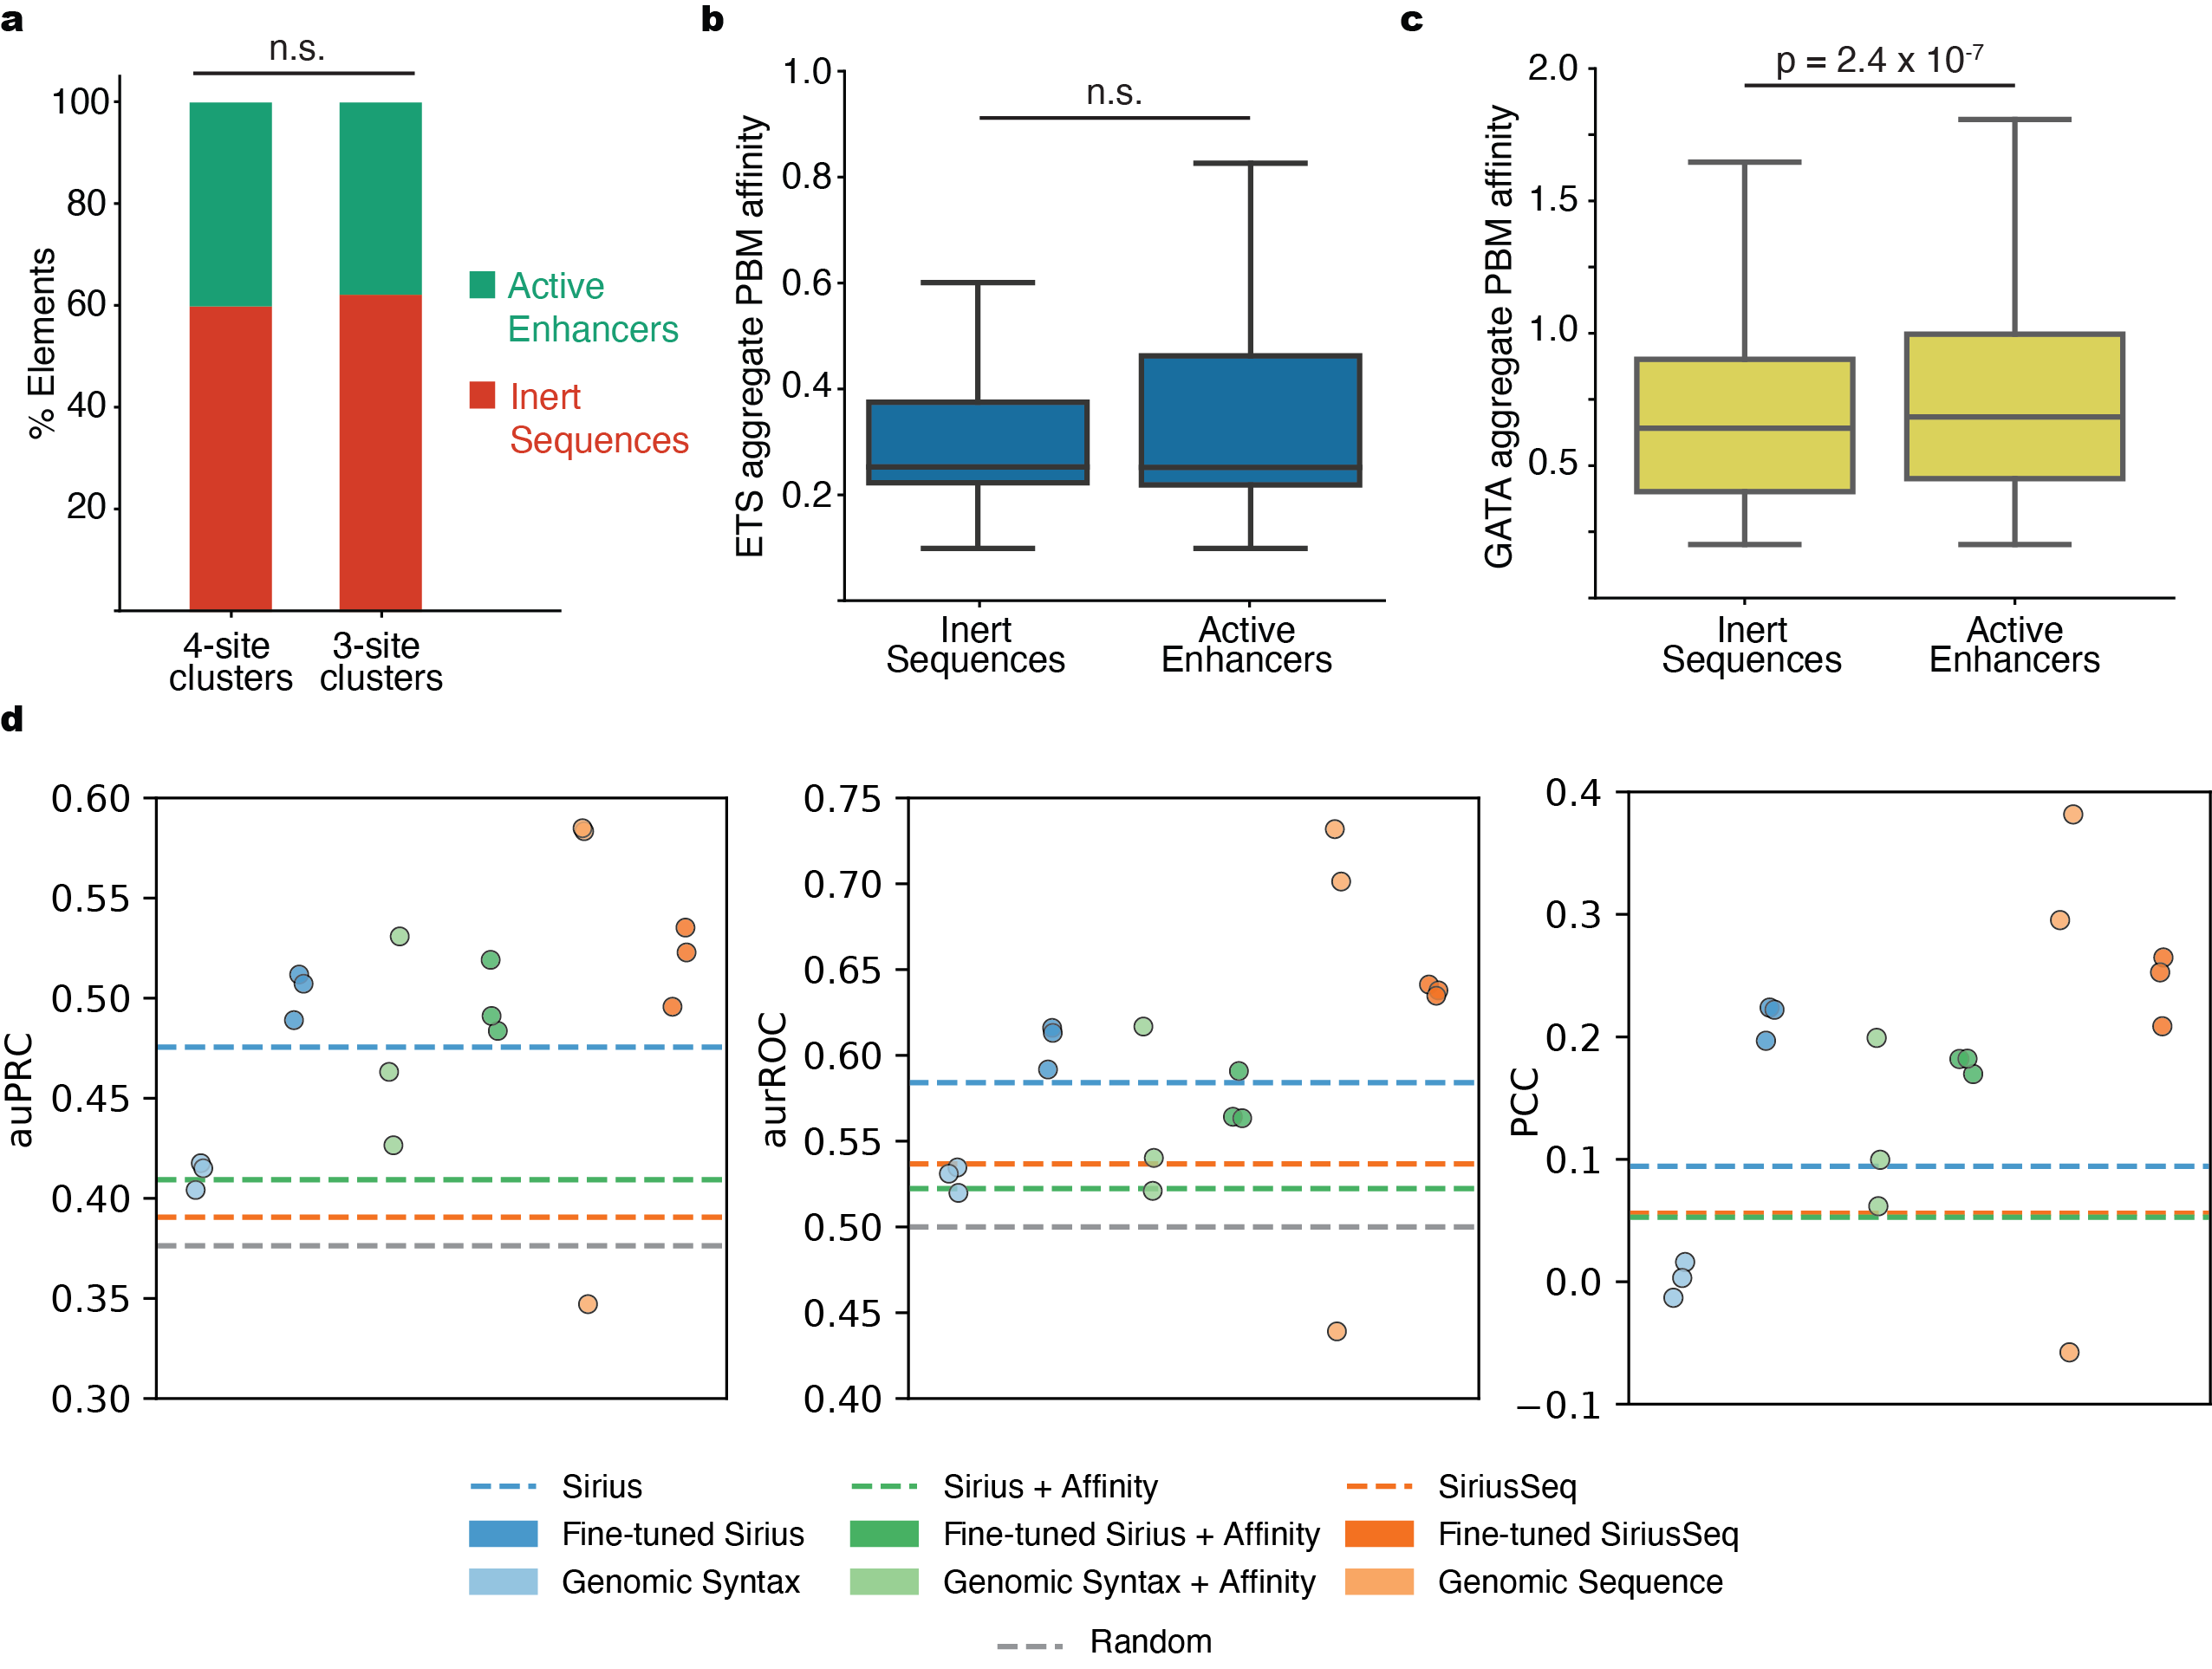
\includegraphics[width=0.88\textwidth]{2_figures-and-files/SuppFig15.png}
    \caption[Additional model training and evaluation.]{\textbf{Additional model training and evaluation.} \textbf{a)} 3-site and 4-site genomic clusters have a similar proportion of active enhancers and inert elements and are not significantly different (n.s.) by a Fisher’s exact test. \textbf{b)} Aggregate affinity of ETS and \textbf{c)} GATA across inert sequences and active enhancers within the library. The aggregate affinities are slightly increased in active elements. For GATA \textbf{c)}, this effect is significant (Mann-Whitney U test). \textbf{d)} Predictive performance on genomic cluster test set across three metrics: left, area under the precision-recall curve (auPRC); middle, area under the receiver operating characteristic curve (auROC); right, Pearson correlation coefficient (PCC). Dashed lines indicate models trained on the OSL library (single fold). All models trained on genomic library sequences were trained across three folds (i.e., each point corresponds to a fold).}
    \label{fig:2 supplementary_15}
\end{figure}

\begin{figure}[p]
    \centering
    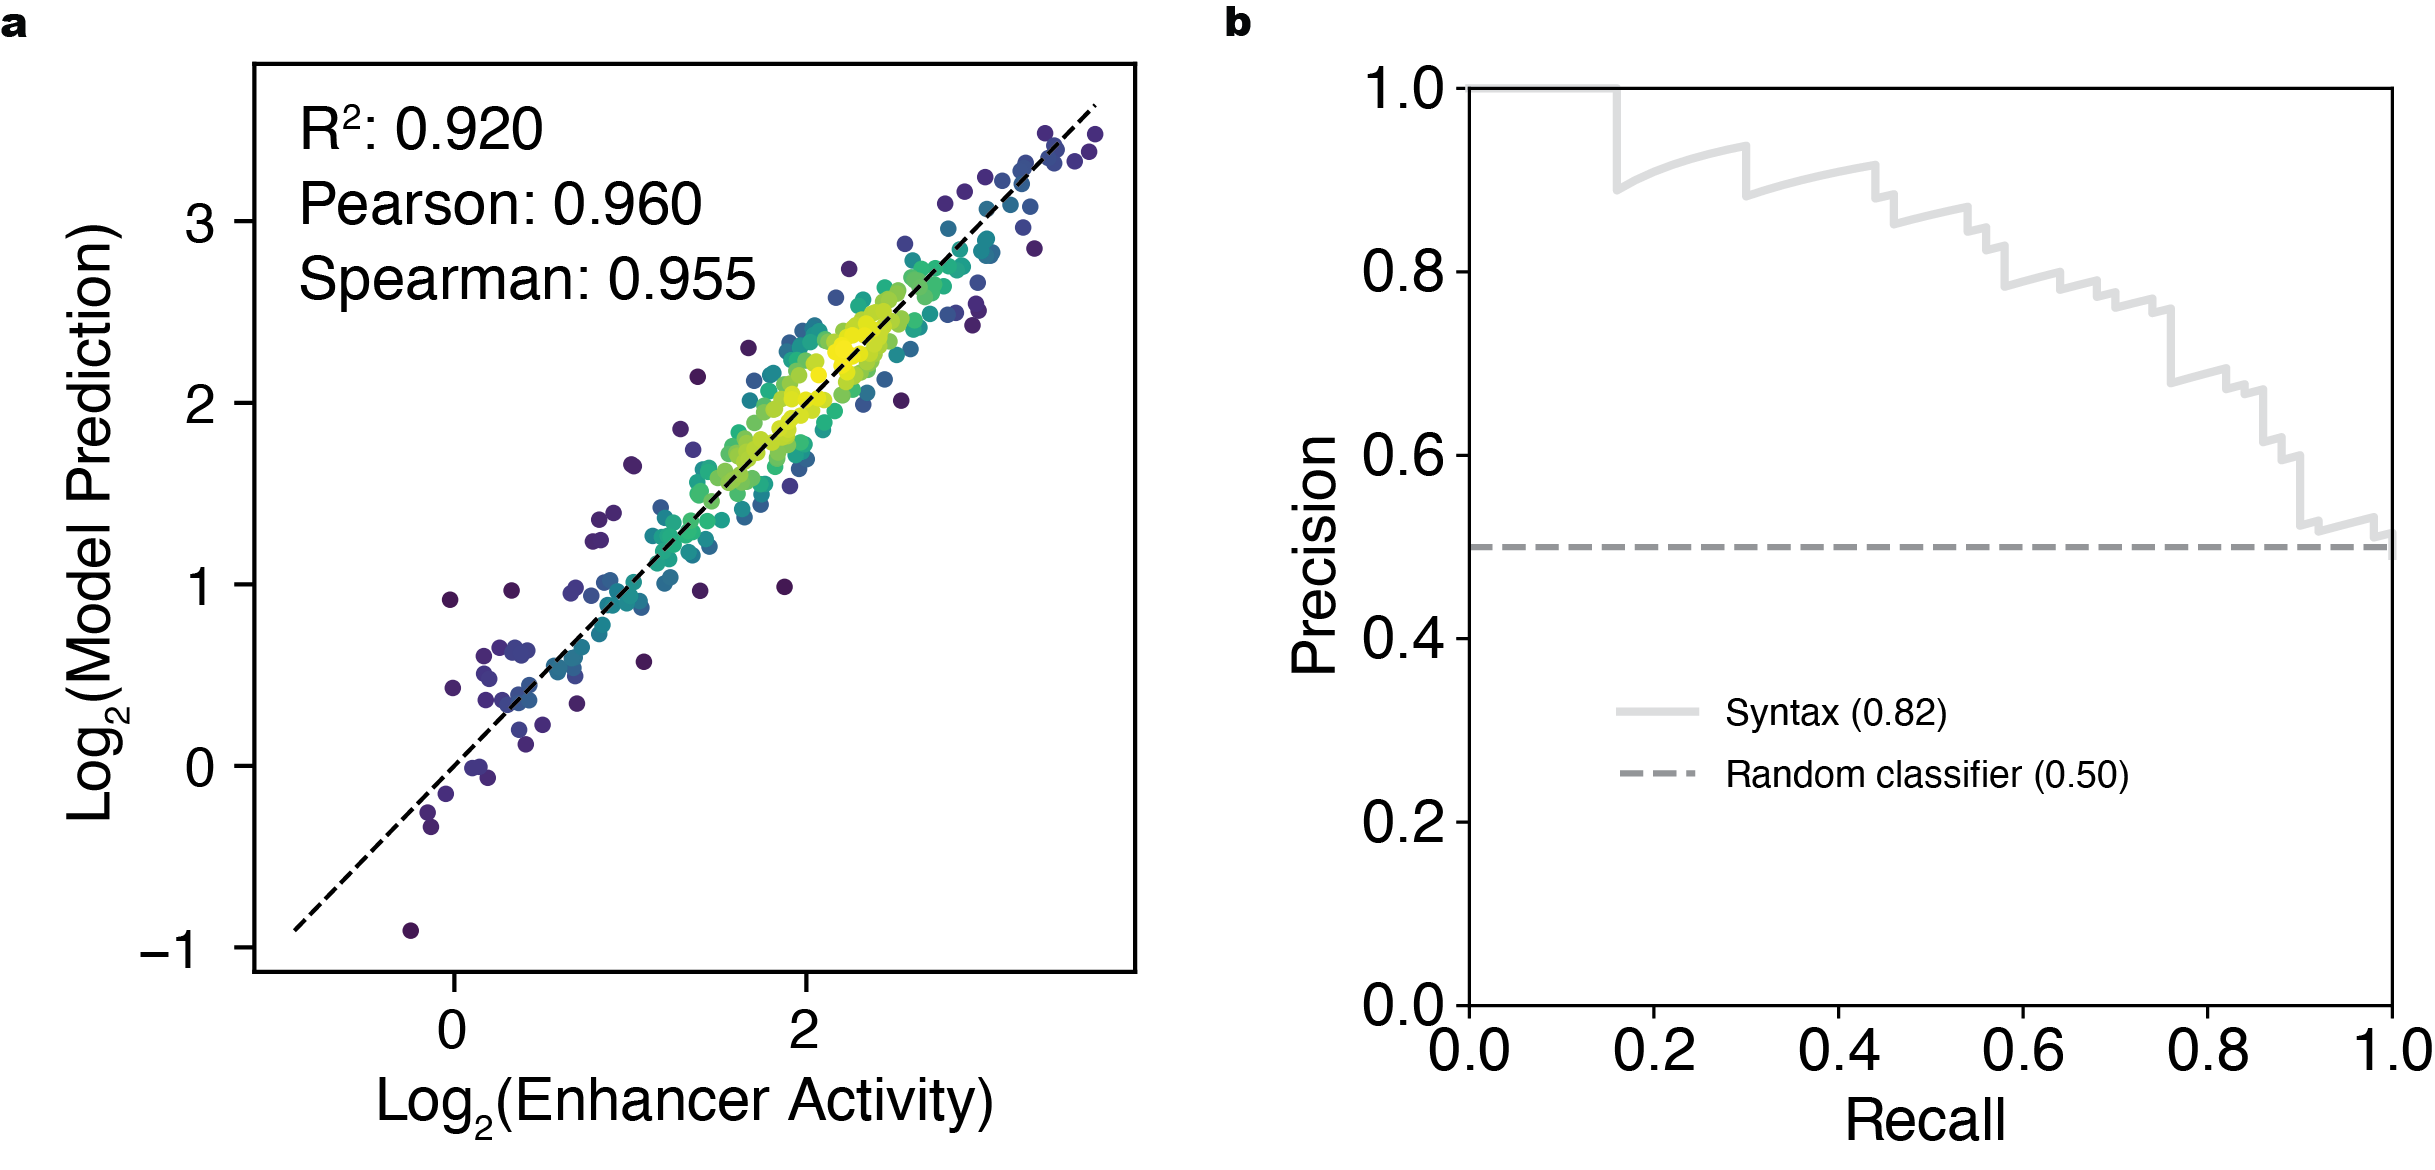
\includegraphics[width=0.88\textwidth]{2_figures-and-files/SuppFig16.png}
    \caption[Assessing the generalizability of the syntax encoding on pluripotency TF synthetic element library in mESC.]{\textbf{Assessing the generalizability of the syntax encoding on pluripotency TF synthetic element library in mESC.} \textbf{a)} Scatterplot of enhancer activity (x-axis) vs model predictions (y-axis) for model trained on synthetic library of four pluripotency transcription factors in mouse embryonic stem cells (mESCs). Percentage of variance explained (R²), Pearson correlation coefficient (PCC) and Spearman’s $rho$ are annotated. \textbf{b)} Precision-recall curve for syntax + affinity model trained on genomic sequence library in mESCs. Areas under the precision-recall curve (auPRC) are indicated in parentheses.}
    \label{fig:2 supplementary_16}
\end{figure}

\appendix{}

\chapter{Supplemental Material for Chapter \ref{chap:chapter 3}}

%%%%%%%%%%%%%%%%%%%%%%%%%%%%%%%%%%%%%%%%%%%%%%%%%%%%%%%%%%%%%%%%%%%%%%%%%%%%%%%%
\section{Supplementary Figures}
%%%%%%%%%%%%%%%%%%%%%%%%%%%%%%%%%%%%%%%%%%%%%%%%%%%%%%%%%%%%%%%%%%%%%%%%%%%%%%%%

\begin{figure}[p]
    \centering
    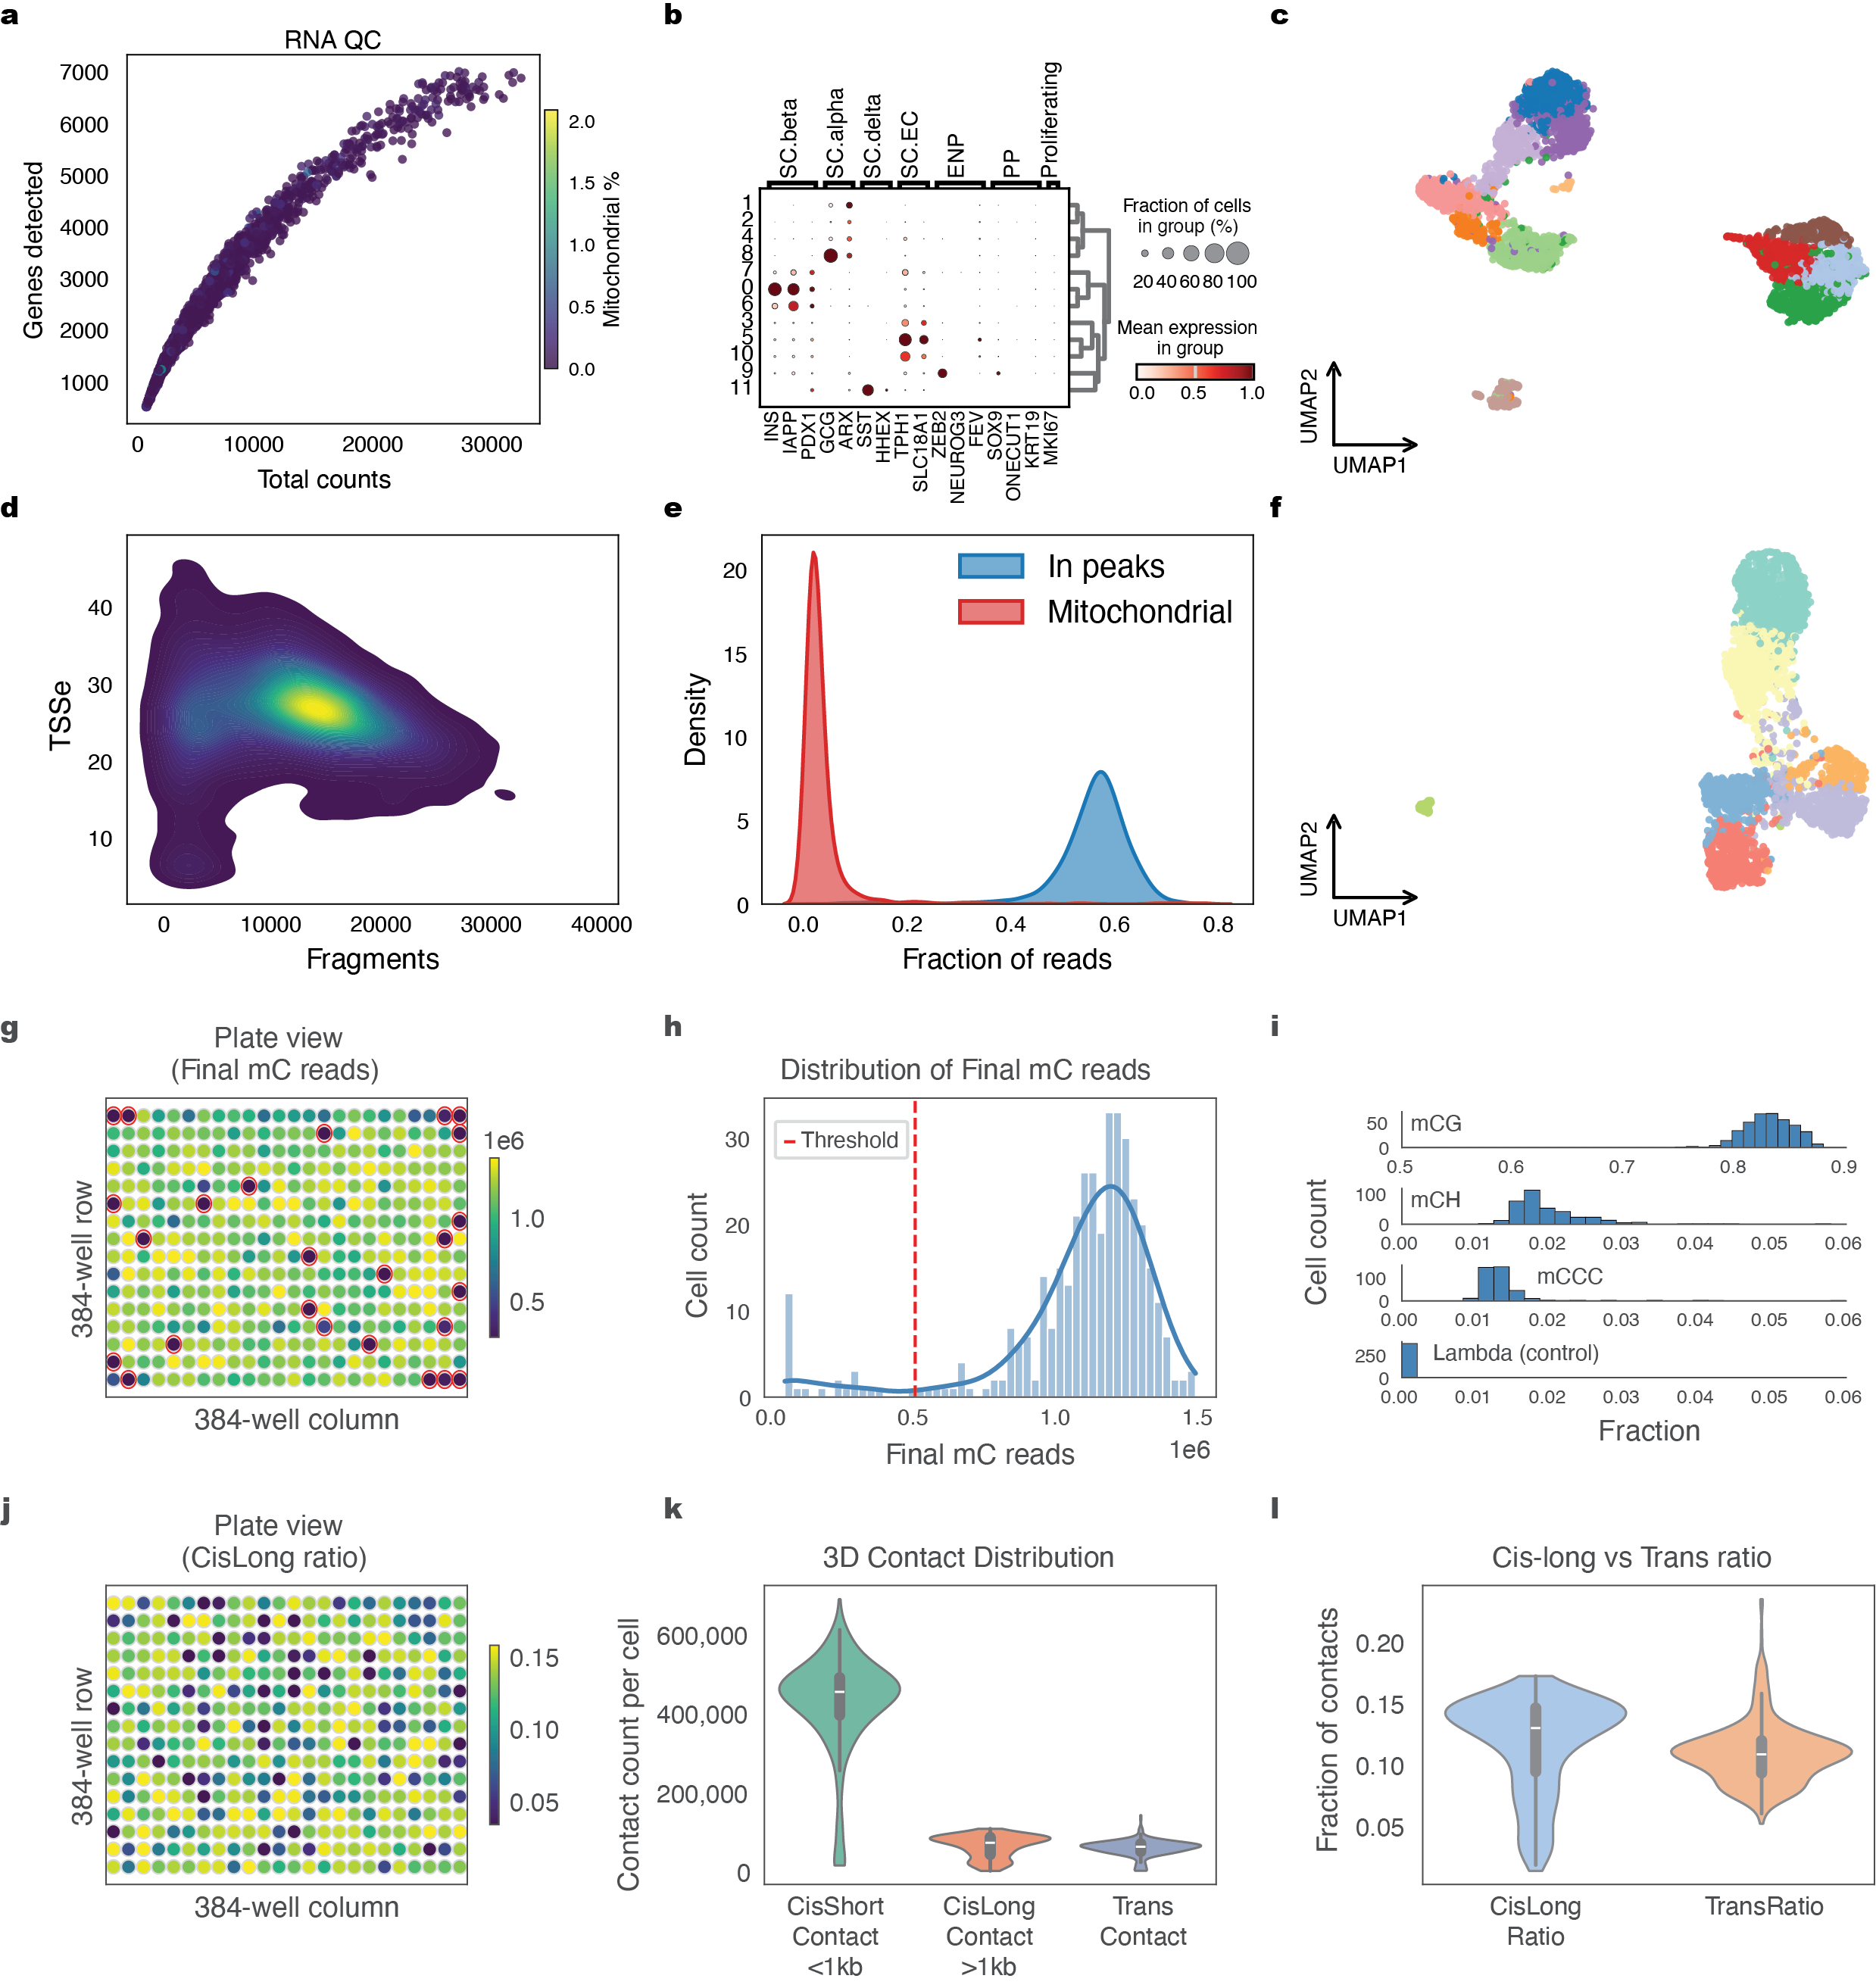
\includegraphics[width=\textwidth]{3_figures-and-files/ExtendedFig1.png}
    \caption[Quality control across molecular modalities]{\textbf{Quality control metrics across molecular modalities for a representative sample (15-1, control, 6 hr)}. \textbf{a}, RNA QC scatterplot showing total UMI counts versus number of genes detected per cell, colored by mitochondrial read percentage. \textbf{b}, Dot plot of marker gene expression across Leiden clusters. \textbf{c}, UMAP embedding of RNA-seq data colored by Leiden clusters. \textbf{d}, ATAC QC density plot of TSS enrichment versus number of fragments per cell. \textbf{e}, Distribution of fraction of reads mapping to peaks (blue) and mitochondrial genome (red) for ATAC data. \textbf{f}, UMAP embedding of ATAC-seq data colored by Leiden clusters. \textbf{g}, Plate layout showing the number of final methylation (mC) reads per well. \textbf{h}, Histogram of final mC read counts per cell, with dashed line indicating threshold for filtering. \textbf{i}, Histogram of global methylation metrics (mCG, mCH, and $\lambda$ spike-in control). \textbf{j}, Plate layout showing cis-long contact ratio per well for 3C data. \textbf{k}, Violin plots of total 3D chromatin contacts per cell, stratified into cis-short (<1 kb), cis-long (>1 kb), and trans interactions. \textbf{l}, Distribution of cis-long versus trans contact ratios per cell.}
    \label{fig:3 supplementary_1}
\end{figure}

\begin{figure}[p]
    \centering
    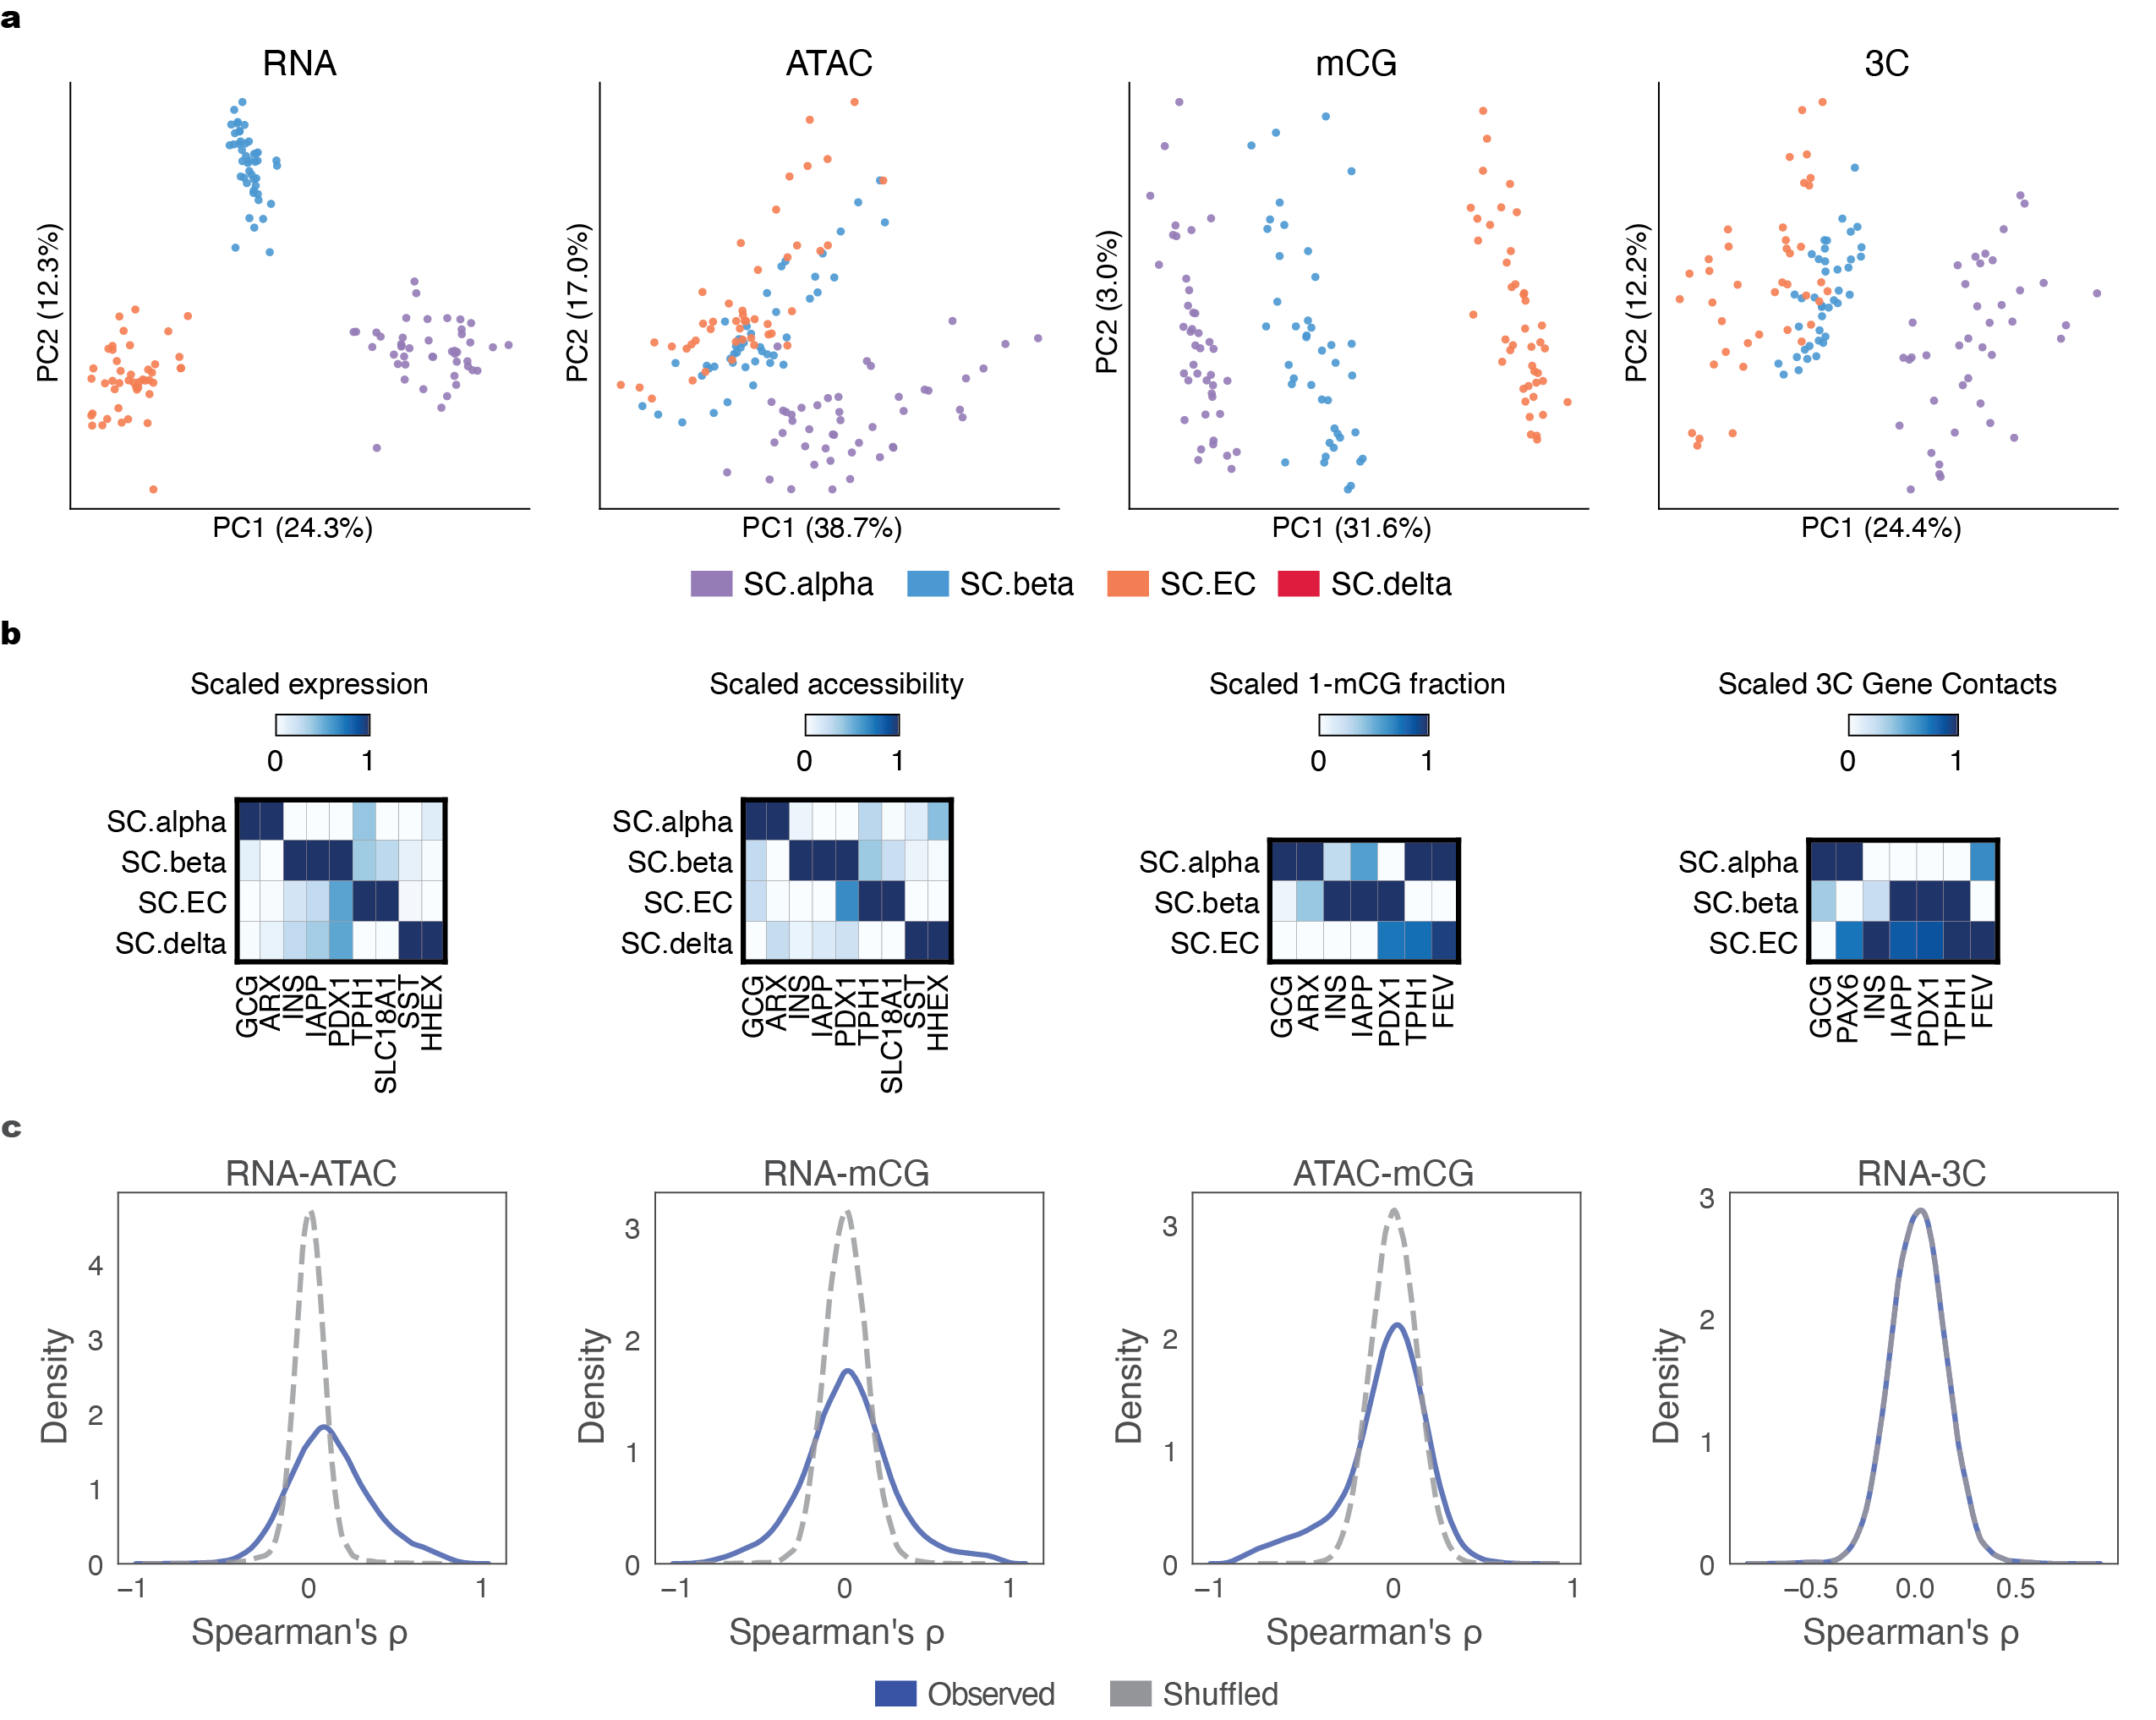
\includegraphics[width=\textwidth]{3_figures-and-files/ExtendedFig2.png}
    \caption[Modality comparison of pseudobulked profiles]{\textbf{Modality comparison of pseudobulked molecular profiles in SC-islet organoids}. \textbf{a}, Principal component analysis of pseudobulk profiles for each cell type across four molecular modalities: mRNA expression (RNA), chromatin accessibility (ATAC), DNA methylation (mCG), and 3D chromatin contacts (3C). Percentage of variance explained are annotated on axes. Points are colored by cell type. \textbf{b}, Heatmaps showing scaled expression, accessibility, methylation, and 3C contact signals across selected marker genes, stratified by cell type. \textbf{c}, Distributions of pairwise Spearman correlations between molecular modalities across genes (blue: observed; gray: shuffled null distribution).}
    \label{fig:3 supplementary_2}
\end{figure}

\begin{figure}[p]
    \centering
    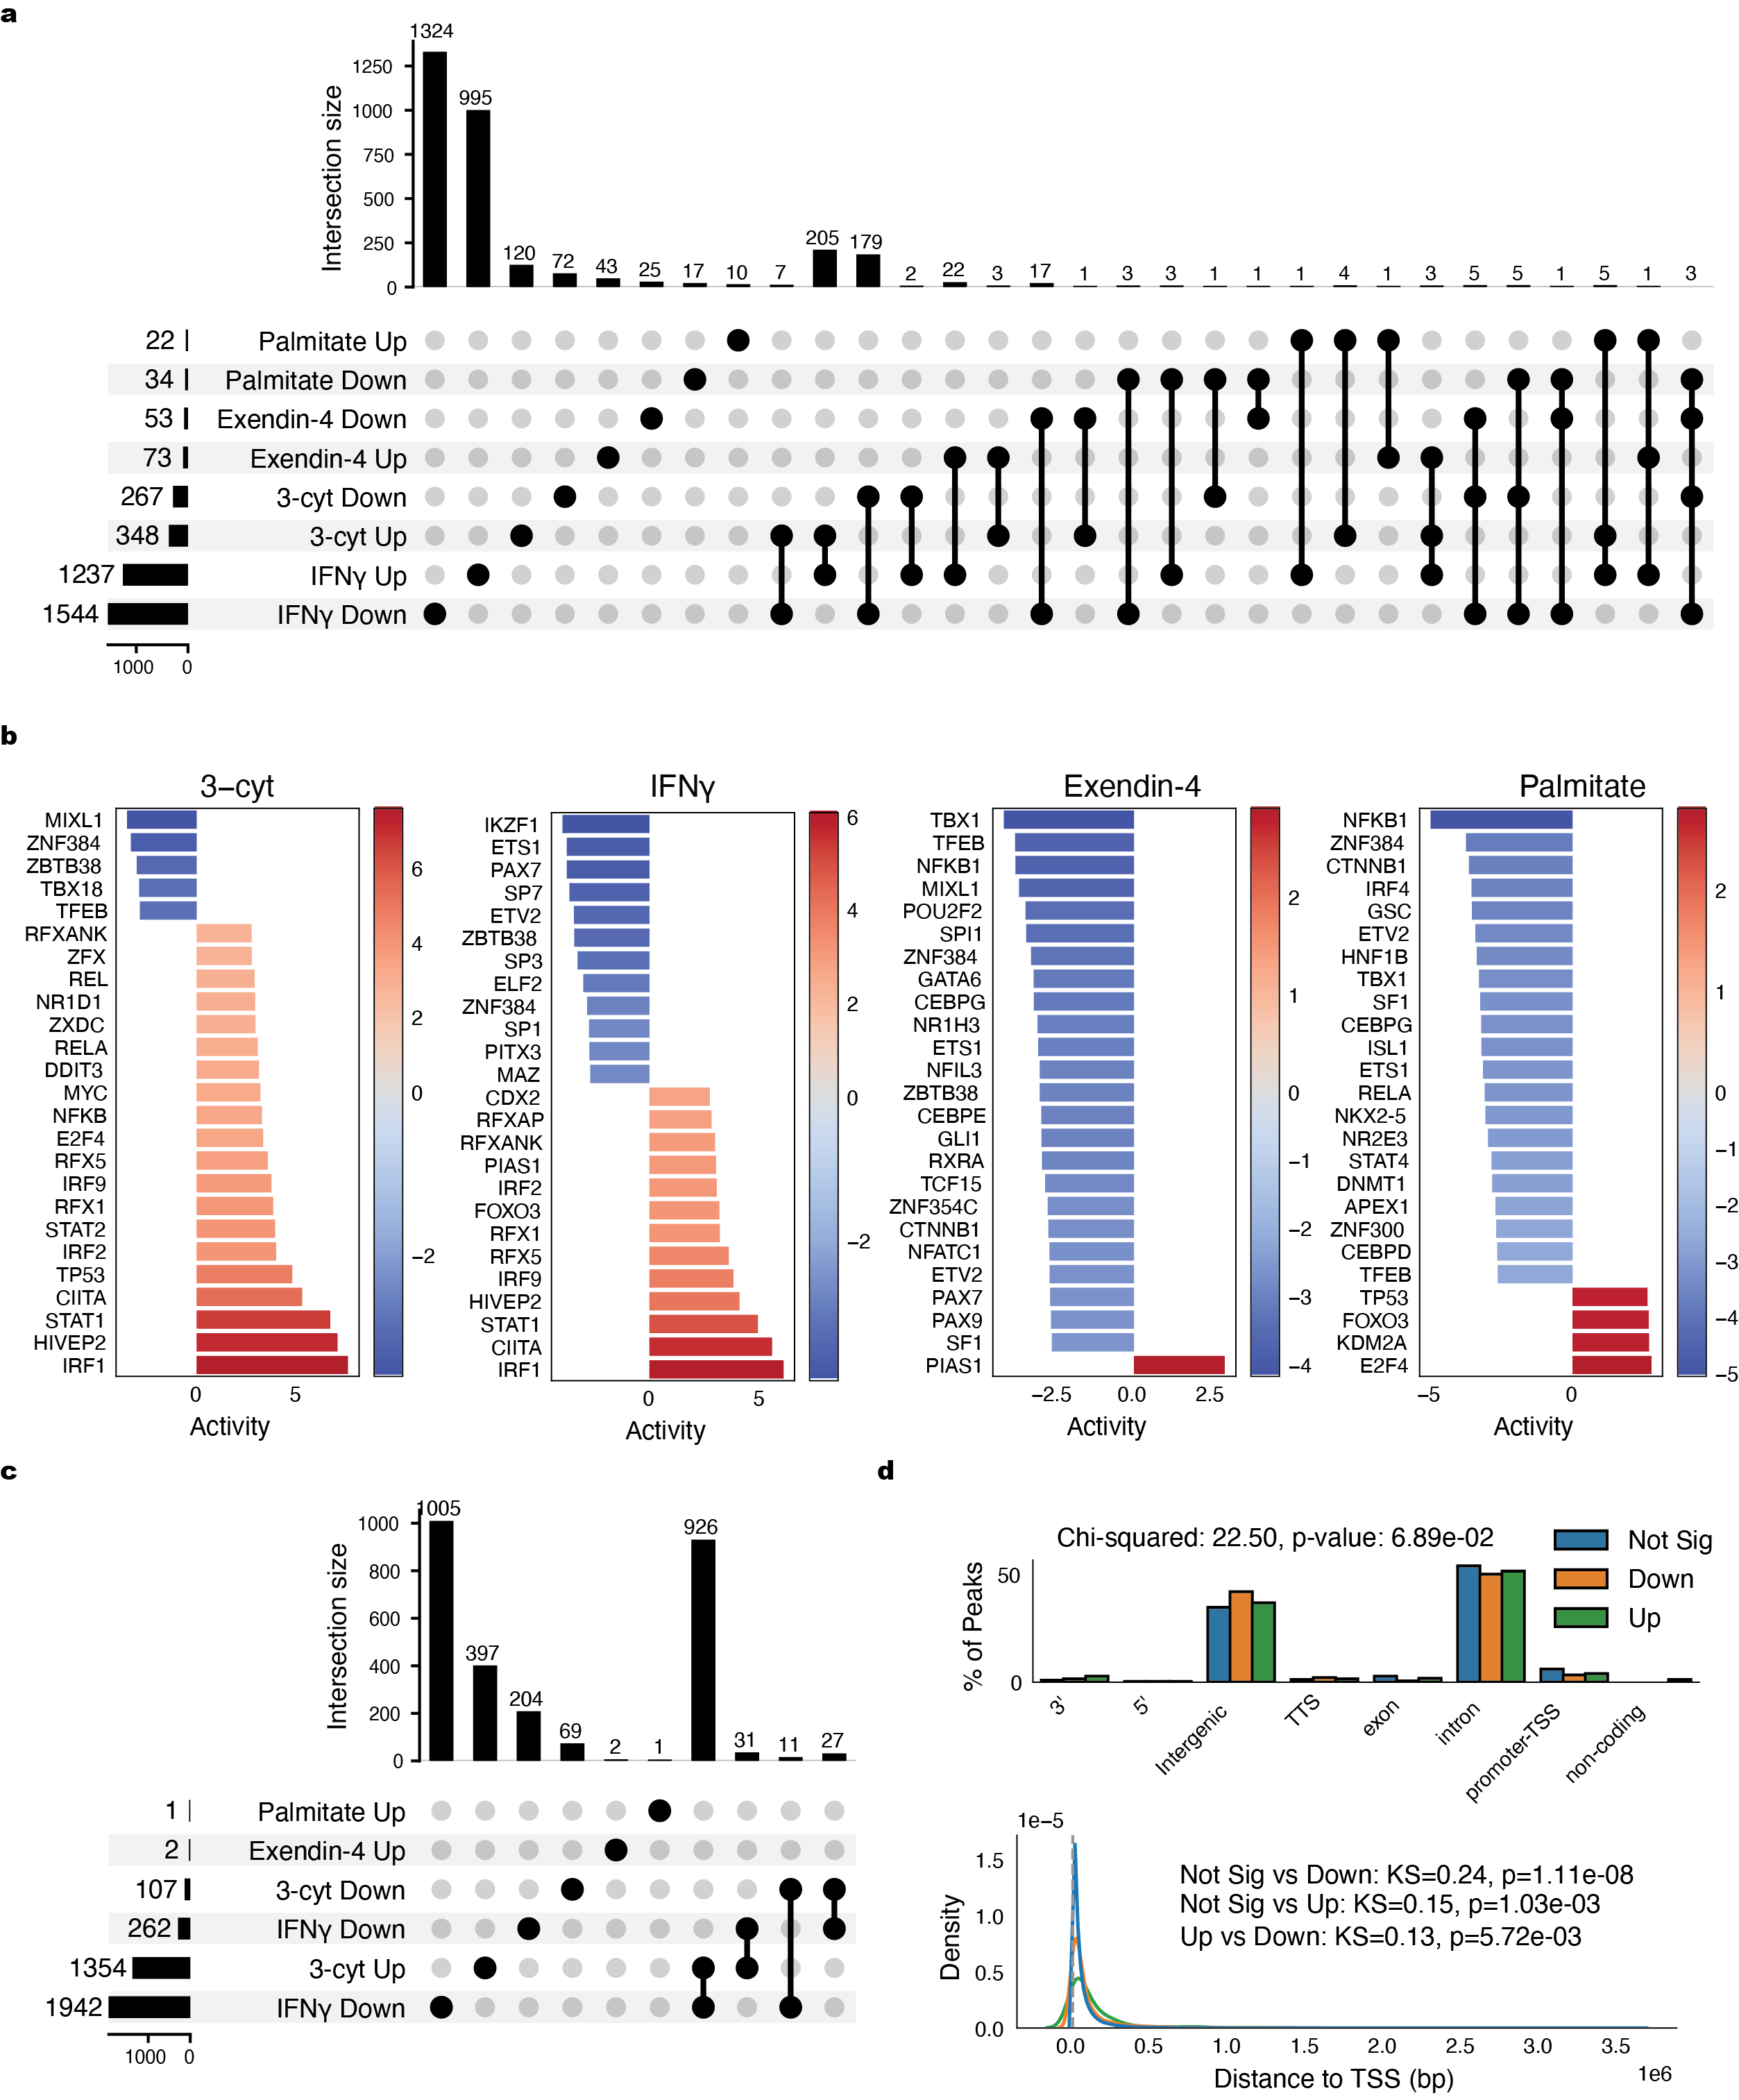
\includegraphics[width=\textwidth]{3_figures-and-files/ExtendedFig3.png}
    \caption[Stimulus-specific and shared SC-beta cell responses]{\textbf{Stimulus-specific and shared multiome responses in SC-beta cells}. \textbf{a}, UpSet plot summarizing the overlap of differentially expressed gene (DEG) sets across treatment conditions. Bars show the number of DEGs (FDR < 0.05 for cytokines, < 0.25 for others) up- or down-regulated in each condition and their intersections. The largest overlaps are observed between cytokine treatments (3-cyt, IFNg), with minimal overlap across non-inflammatory stimuli. \textbf{b}, Inferred transcription factor activity across conditions using decoupleR. \textbf{c}, UpSet plot of DARs stratified by direction of regulation. \textbf{d}, Genomic annotation (top) and TSS-distance distribution (bottom) for DARs. Chi-square p-value is indicated. Pairwise Kolmogorov–Smirnov test statistics and p-values are annotated.}
    \label{fig:3 supplementary_3}
\end{figure}


%%%%%%%%%%%%%%%%%%%%%%%%%%%%%%%%%%%%%%%%%%%%%%%%%%%%%%%%%%%%%%%%%%%%%%%%%%%%%%%
% End of the Dissertation
%%%%%%%%%%%%%%%%%%%%%%%%%%%%%%%%%%%%%%%%%%%%%%%%%%%%%%%%%%%%%%%%%%%%%%%%%%%%%%%%
\backmatter{}
\bibliographystyle{unsrtnat} 
\bibliography{bibliography}

\end{document}
